\documentclass{thesisclass}
% Based on thesisclass.cls of Timo Rohrberg, 2009
% ----------------------------------------------------------------
% Thesis - Main document
% ----------------------------------------------------------------
% No empty in-between chapters, remove this line if desired for double-page printing
\let\cleardoublepage\clearpage

%% -------------------------------
%% |  Information for PDF file   |
%% -------------------------------
\hypersetup{
 pdfauthor={Nina Zimbel},
 pdftitle={Generierung von Wirbeltierskeletten},
 pdfsubject={Not set},
 pdfkeywords={Not set}
}


%% ---------------------------------
%% | Information about the thesis  |
%% ---------------------------------

\newcommand{\myname}{Nina Zimbel}
\newcommand{\mytitle}{Prozedurale Generierung von Wirbeltierskeletten}
\newcommand{\myinstitute}{Institut für Visualisierung und Datenanalyse,\\ Lehrstuhl für Computergrafik}

\newcommand{\reviewerone}{Prof. Dr.-Ing. Carsten Dachsbacher}
\newcommand{\reviewertwo}{Prof. Dr. Hartmut Prautzsch}
\newcommand{\advisor}{Dr. Johannes Schudeiske}
%\newcommand{\advisortwo}{?}

\newcommand{\timestart}{\date{01.12.2019}}
\newcommand{\timeend}{\date{31.05.2020}}
\newcommand{\submissiontime}{DD. MM. 20XX}


%% --------------------------------
%% | Bibliography                 |
%% --------------------------------

%% Use biber instead of BibTeX, see README
\usepackage[citestyle=numeric,style=numeric,backend=biber]{biblatex}
\addbibresource{bibliography.bib}

%% --------------------------------
%% | Appendix                     |
%% --------------------------------
\usepackage[titletoc]{appendix}

%% ---------------------------------
%% | ToDo Marker - only for draft! |
%% ---------------------------------
% Remove this section for final version!
\setlength{\marginparwidth}{20mm}

\newcommand{\margtodo}
{\marginpar{\textbf{\textcolor{red}{ToDo}}}{}}

\newcommand{\todo}[1]
{{\textbf{\textcolor{red}{(\margtodo{}#1)}}}{}}


%% --------------------------------
%% | Old Marker - only for draft! |
%% --------------------------------
% Remove this section for final version!
\newenvironment{deprecated}
{\begin{color}{gray}}
{\end{color}}


%% --------------------------------
%% | Shorcuts                     |
%% --------------------------------
\newcommand{\zb}{z.\,B.\ }
\newcommand{\dash}{d.\,h.\ }
\newcommand{\va}{v.\,a.\ }
\newcommand{\ua}{u.\,a.\ }
\newcommand{\bzw}{bzw.\ }
\newcommand{\etc}{etc.\ }

%% --------------------------------
%% | Settings for word separation |
%% --------------------------------
% Help for separation:
% In german package the following hints are additionally available:
% "- = Additional separation
% "| = Suppress ligation and possible separation (e.g. Schaf"|fell)
% "~ = Hyphenation without separation (e.g. bergauf und "~ab)
% "= = Hyphenation with separation before and after
% "" = Separation without a hyphenation (e.g. und/""oder)

% Describe separation hints here:
\hyphenation{
% Pro-to-koll-in-stan-zen
% Ma-na-ge-ment  Netz-werk-ele-men-ten
% Netz-werk Netz-werk-re-ser-vie-rung
% Netz-werk-adap-ter Fein-ju-stier-ung
% Da-ten-strom-spe-zi-fi-ka-tion Pa-ket-rumpf
% Kon-troll-in-stanz
}


%% ------------------------
%% |    Including files   |
%% ------------------------
% Only files listed here will be included!
% Userful command for partially translating the document (for bug-fixing e.g.)
%\includeonly{%
%titlepage,
%content,
%appendix
%}


%%%%%%%%%%%%%%%%%%%%%%%%%%%%%%%%%
%% Here, main documents begins %%
%%%%%%%%%%%%%%%%%%%%%%%%%%%%%%%%%
\begin{document}

% Remove the following line for German text
%\selectlanguage{ngerman}

\frontmatter
\pagenumbering{roman}
%% titlepage.tex
%%

% coordinates for the bg shape on the titlepage
\newcommand{\diameter}{20}
\newcommand{\xone}{-15}
\newcommand{\xtwo}{160}
\newcommand{\yone}{15}
\newcommand{\ytwo}{-253}

\begin{titlepage}
% bg shape
\begin{tikzpicture}[overlay]
\draw[color=gray]  
 		 (\xone mm, \yone mm)
  -- (\xtwo mm, \yone mm)
 arc (90:0:\diameter pt) 
  -- (\xtwo mm + \diameter pt , \ytwo mm) 
	-- (\xone mm + \diameter pt , \ytwo mm)
 arc (270:180:\diameter pt)
	-- (\xone mm, \yone mm);
\end{tikzpicture}
	\begin{textblock}{10}[0,0](4,2.5)
		
\includegraphics[width=.3\textwidth]{logos/KITLogo_german.pdf}
	\end{textblock}
	\changefont{phv}{m}{n}	% helvetica	
	\vspace*{3.5cm}
	\begin{center}
		\Huge{\mytitle}
		\vspace*{2cm}\\
		\Large{
			Masterarbeit von
		}\\
		\vspace*{1cm}
		\huge{\myname}\\
		\vspace*{1cm}
		\Large{
			An der Fakult\"at f\"ur Informatik
			\\
			\myinstitute
		}\\
		\vspace*{1cm}
		\Large{\today}
	\end{center}
	\vspace*{1cm}
\Large{
\begin{center}
\begin{tabular}[ht]{l c l}
 % Gutachter sind die Professoren, die die Arbeit bewerten. 
 \iflanguage{english}{Reviewer}{Erstgutachter}: & \hfill  & \reviewerone\\
 \iflanguage{english}{Second reviewer}{Zweitgutachter}: & \hfill  & \reviewertwo\\
 \iflanguage{english}{Advisor}{Betreuender Mitarbeiter}: & \hfill  & \advisor\\
 %\iflanguage{english}{Second advisor}{Zweiter betreuender Mitarbeiter}: & \hfill  & \advisortwo\\
 % Der zweite betreuende Mitarbeiter kann weggelassen werden. 
\end{tabular}
\end{center}
}


\vspace{2cm}


\begin{textblock}{10}[0,0](4,16.8)
\tiny{ 
		{KIT -- Universität des Landes Baden-Württemberg und nationales Forschungszentrum der Helmholtz-Gesellschaft}
}
\end{textblock}

\begin{textblock}{10}[0,0](14,16.75)
\large{
	\textbf{www.kit.edu} 
}
\end{textblock}

\end{titlepage}

\blankpage


%% -------------------
%% |   Directories   |
%% -------------------
\tableofcontents
\blankpage


%% -----------------
%% |   Main part   |
%% -----------------
\mainmatter
\pagenumbering{arabic}
%-------------------
%-------------------
\chapter{Einleitung}

Wirbeltiere sind allgegenwärtig, sowohl im alltäglichen Leben, als auch in Computerspielen und Filmen. Es besteht also ein stetiger Bedarf an 3D-Modellen von Wirbeltieren. Dieser wird in den meisten Fällen durch Künstler gedeckt, die viel Zeit und Arbeit in die Modelle stecken. Algorithmen, die diese Abläufe vereinfachen könnten, beispielsweise durch prozedurale Generierung, gibt es nicht viele.

% Ziel
Das Ziel dieser Arbeit ist es den Arbeitsaufwand der Künstler zu verringern, indem eine Möglichkeit geschaffen wird Wirbeltierskelette automatisiert zu generieren. Diese Skelette können dann die Grundlage für die Modellierung eines kompletten Wirbeltiers bilden.
Einerseits können sie dabei als Inspiration dienen. Sie können einen Anhaltspunkt zu Körperform und Proportionen bieten und zu möglichen Bewegungsabläufen. Außerdem kann schnell eine große Auswahl an Skeletten generiert werden.\\
Andererseits können die Skelette eine Grundlage für Modelle bilden, die zusätzlich auch Muskeln und Haut simulieren.
In beiden Fällen darf das Modell nicht zu abstrakt sein, da es sonst zu wenig Informationen zum Aufbau des konkreten Tiers liefert.\\
Es soll also ein Skelett generiert werden, dass genug Knochen enthält um realistisch zu wirken, aber auch nicht zu viele um den Aufwand für die Generierung und die Programmierung des Algorithmus im Rahmen zu halten.

% Warum nur Wirbeliere?
Der Grund dafür, dass sich diese Arbeit auf Wirbeltierskelette einschränkt ist, dass der Skelettaubau von Wirbeltieren nicht zu stark variiert. 
Je mehr Details betrachtet werden, desto mehr Unterschiede gibt es, aber der grobe Aufbau ist bei allen Wirbeltieren sehr ähnlich. Die Grundlagen zur Biologie der Wirbeltiere, die für diese Arbeit notwendig sind, werden in Kapitel \ref{chapter:biology} vorgestellt, die technischeren Grundlagen in Kapitel \ref{chapter:basics}.

% Methoden+Aufbau
Die wichtigsten Schritte des Algorithmus werden im Folgenden kurz angerissen, um einen Überblick über die Arbeit zu geben.
Die Datengrundlage für den Algorithmus schafft eine \emph{Principal Component Analyis} (Hauptkomponentenanalyse) auf annotierten 2D-Skelett"-bildern (Kapitel \ref{chapter:pca}). 
Die Knochen des Skeletts werden dann mit Hilfe einer kontextfreien Grammatik generiert und gleichzeitig angeordnet (Kapitel \ref{chapter:skeleton_generation}). 
Zum Schluss wird aus existierenden 3D-Modellen von einzelnen Knochen ein 3D-Modell des generierten Skeletts erstellt (Abschnitt \ref{bone_models})).\\
Zunächst generiert der Algorithmus zufällige Skelette. Es werden aber auch Benutzereingaben, \zb zur Anzahl der Extremitäten, berücksichtigt oder Variationen zu schon bestehenden Skeletten generiert (Kapitel \ref{chapter:additional_features}). \\
Zusätzliche Informationen zu Implementierungsdetails sind in Kapitel \ref{chapter:implementation_detail} zu finden und abgerundet wird die Arbeit mit Fazit und Ausblick in Kapitel \ref{chapter:conclusion}.

% Aufbau der Arbeit
% In Kapitel \ref{chapter:biology} werden zunächst einige Grundlagen zur Biologie der Wirbeltiere vorgestellt, die später zum Verständnis des Algorithmus nötig sind. Die technischeren Grundlagen werden in Kapitel \ref{chapter:basics} erklärt.\\
% Kapitel \ref{chapter:pca} widmet sich der \emph{Principal Component Analyis}. Es wird beschrieben auf welchen Daten und mit welchen Ergebnissen sie im Rahmen des Algorithmus angewandt wird. Diese Analyse ist auch der erste Schritt des Algorithmus, der in Kapitel \ref{chapter:skeleton_generation} ausführlich beschrieben wird. Zusätzliche Funktionen, wie das Laden und Speichern von Skeletten oder die Erzeugung von Variationen zu gespeicherten Skeletten werden in Kapitel \ref{chapter:additional_features} vorgestellt.
% Kapitel \ref{chapter:implementation_detail} versammelt alle Details zur Implementierung und abgerundet wird die Arbeit mit Fazit und Ausblick in Kapitel \ref{chapter:conclusion}.



%---------------------------------
%---------------------------------
\chapter{Biologie der Wirbeltiere}
\label{chapter:biology}
% eventuell als Abschnitt in "`Grundlagen"'?

\begin{center}
 \begin{minipage}{12cm}
  \emph{"`Nichts anderes in der Natur hat eine herrlichere Struktur als der Körper der Wirbeltiere."'}
 
  --- "`Vergleichende und funktionelle Anatomie der Wirbeltiere"' \cite{Vergleichende_Anatomie}, S.\ 1
 \end{minipage}
\end{center}

Dieses Kapitel soll einen Überblick über die biologische Beschaffenheit der Wirbeltiere geben. Da dies keine biologische Arbeit ist, werden nur diejenigen Merkmale und Eigenschaften weiter ausgeführt, die im Folgenden zum Verständnis nötig sind.

% Definition
Wirbeltiere, oder auch Vertebrata, sind Tiere mit einer skelettartigen Schädelkapsel, einem Cranium. Deshalb werden sie auch Schädeltiere oder Craniota genannt.\\
Auf den ersten Blick ist diese Definition etwas überraschend, da als  Haupteigenschaft nicht die Wirbelsäule, sondern der Schädel genannt wird. Das liegt daran, dass zu den Wirbeltieren auch einige Tiere gezählt werden, die gar keine Wirbelsäule sondern "`nur"' eine Chorda dorsalis besitzen. Die Chorda dorsalis besteht aus weichem Gewebe, nicht aus Knochen. Sie ist das Achsenskelett der Chordatiere, einem Tierstamm, zu dem auch die Wirbeltiere gehören. (\cite{Vergleichende_Anatomie}, S.27 f.)\\
Hier in dieser Arbeit soll es aber nur um Wirbeltiere mit Wirbelsäule gehen.

% 5 Klassen
Es gibt fünf große Gruppen von Wirbeltieren. Die historisch ersten Wirbeltiere sind die Fische. Danach entwickelten sich die Tetrapoden, Wirbeltiere mit vier Gliedmaßen, zu denen alle anderen Gruppen gehören. Zunächst entstanden die Amphibien, die noch nicht vollkommen terrestrisch leben. Daraus entwickelten sich die Reptilien, die erste Klasse der Wirbeltiere, die alle Strukturen besitzt um vollkommen an Land zu leben. (Es gibt aber auch Reptilien die trotzdem wieder im Wasser leben.) Außerdem gibt es noch die Vögel, die sich auf das Fliegen spezialisiert haben, und die Säugetiere, die ihre Jungen säugen. (\cite{Vergleichende_Anatomie}, Kapitel 4)

Auch der Mensch ist ein Säugetier und besitzt eine Wirbelsäule. Da sich Wirbeltiere, vor allem in ihrem Skelett, sehr ähneln, lassen sich viele der im folgenden Abschnitt aufgeführten Eigenschaften des Skeletts, vermutlich leicht "`am eigenen Leib"' nachvollziehen.


%------------------------------------
\section{Das Skelett}
\label{biology_skeleton}

\vspace{0.5cm}
\begin{center}
 \begin{minipage}{12cm}
  \emph{"`Das innere, gelenkige Skelettsystem der Vertebraten ist einzigartig im Tierreich. Es ist das wichtigste aller Organsysteme für das Studium der Wirbeltiermorphologie."'}
  --- \cite{Vergleichende_Anatomie}, S.\ 131
 \end{minipage}
\end{center}


Wirbeltiere haben ein inneres Skelett und ihr Körper ist bilateralsymmetrisch (\cite{Vergleichende_Anatomie}, S.27). Das bedeutet, dass ihre linke Körperseite symmetrisch zur rechten ist. 

% Wirbelsäule
Die \emph{Wirbelsäule} ist je nach Lebensweise des entsprechenden Wirbeltiers aufgebaut. Ein wesentlicher Einflussfaktor auf Form und Aufbau sind die Kräfte, die auf sie wirken. 
Bei Fischen muss die Wirbelsäule dem Druck der starken Axialmuskeln, die seitlich am Körper entlang führen, entgegenwirken.
Bei Tetrapoden sind diese Axialmuskeln zurückgebildet, dafür muss die Wirbelsäule aber der Schwerkraft widerstehen.
Und bei Vögeln ist die Wirbelsäule speziell an den Flug angepasst und deshalb \ua besonders leicht. (\cite{Vergleichende_Anatomie}, Abschnitt 9.2, S.\ 168 ff.)

% Wirbelanzahl
Auch die Anzahl der Wirbel unterscheidet sich teilweise erheblich. 
Die Halswirbelsäule ist \zb bei den Fischen noch gar nicht herausgebildet. Amphibien haben einen Wirbel, der für die Beweglichkeit des Kopfes zuständig ist. Bei Reptilien ist die Halsregion meist schon stärker abgesetzt. Säugetiere haben, bis auf wenige Ausnahmen, genau $7$ Halswirbel, egal wie lang der Hals ist. Vögel haben die meisten Halswirbel, nämlich $10$ bis maximal $31$ beim Trauerschwan \cite{WikipediaVogelskelett}, meistens aber zwischen $15$ und $20$. (siehe auch \cite{Vergleichende_Anatomie}, Abschnitt 9.2)

Ebenso unterscheidet sich die Anzahl der Wirbel in anderen Teilen der Wirbelsäule. Teilweise sind Wirbel sogar miteinander zu einem größeren Knochen verwachsen. Betrachtet man nur die Gruppe der Säugetiere, so kommt man auf etwa $12$ bis $14$ Brustwirbel, $5$ bis $7$ Lendenwirbel, $3$ bis $5$ Kreuzwirbel und $4$ bis $22$ Schwanzwirbel \cite{AnatomieKuenstler}.

% Wirbelform
Auch die Form der einzelnen Wirbel unterscheidet sich sowohl zwischen den verschiedenen Tieren als auch entlang der Wirbelsäule einer einzelnen Art (\cite{Vergleichende_Anatomie}, Abschnitt 9.1 und Abbildung 9.2). Diese Vielfalt in ein Regelwerk zu zwängen, um sie automatisch generieren zu können, erscheint aussichtslos. Deshalb wird hier mit einem Platzhaltern gearbeitet, der für alle Arten von Wirbeln steht.

% Extremitäten
Die \emph{Extremitäten} der Tetrapoden sind nach einem "`Grundbauplan"' aufgebaut (siehe Abbildung \ref{extremities}a). Dieser wird jedoch vielfach abgewandelt. Einige Beispiele sind in Abbildung \ref{extremities}b zu sehen. (\cite{AllgemeineZoologie}, S.\ 487)\\
Bei Fischen haben die Extremitäten keine Verbindung zur Wirbelsäule. Erst Amphibien bilden Schulter- und Beckengürtel aus, da sie zur Fortbewegung an Land nötig sind. (\cite{Vergleichende_Anatomie}, Abschnitt 9.2.3)
Der Einfachheit halber wird hier aber nicht weiter beachtet ob eine Verbindung zur Wirbelsäule besteht, oder nicht. 

 \begin{figure}
  \subfloat[Grundbauplan]{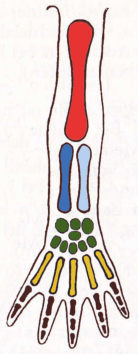
\includegraphics[height=0.35\textheight]{graphics/GrundbauplanExtremitaet_bearbeitet.pdf}} \label{grundbauplan}
  \qquad
  \subfloat[Beispiele]{\includegraphics[height=0.35\textheight]{graphics/ExtremitaetenBeispiele2.pdf}} \label{bsp_extremitaeten}
  
  \caption{Extremitäten von Tetrapoden, Oberarm rot, Speiche dunkelblau, Elle hellblau, Handwurzelknochen grün, Mittelhandknochen gelb, Finderknochen braun\\
  (a) Grundbauplan (\cite{AllgemeineZoologie} S.\ 487, vereinfacht und eingefärbt),\\
  (b) Beispiele für Vordergliedmaßen von Mensch (1), Eidechse (2), Wal (3), Maulwurf (4), Pinguin (5), Pferd (6), Flugsaurier (7), Vogel (8) und Fledermaus (9). \mbox{(\cite{dtvBiologie}, S.\ 474)}}
  \label{extremities}
 \end{figure}

% Extremitätengürtel
Schulter- und Beckengürtel bestehen  jeweils aus mehreren Knochen, die je nach Art mehr oder weniger ausgebildet, unterschiedlich geformt oder sogar komplett zurückgebildet sein können (siehe \cite{Vergleichende_Anatomie}, Absatz 9.7). Um das im Folgenden zu vereinfachen, wird jeder Extremitätengürtel durch einen Knochen repräsentiert. Der Schultergürtel wird durch ein Schulterblatt ersetzt und der Beckengürtel durch einen "`Beckenknochen"'.

% verallgemeinerter und abstrahierter Bauplan
Das Skelett von Wirbeltieren ist im Allgemeinen also ein kompliziertes Konstrukt aus vielen Einzelteilen, die zwischen verschiedenen Arten stark variieren. Um einen Algorithmus zu entwerfen, der Skeletten nachempfundene Gebilde konstruiert, ist es also notwendig ein erheblich vereinfachtes Modell zu erstellen.\\ 
In Abbildung \ref{bauplan_skelett} ist ein verallgemeinerter und abstrahierter Bauplan für Wirbeltiere zu sehen. Er ist reduziert auf die Wirbelsäule, Rippen, Schädel, Extremitäten, Schulterblatt und Beckenknochen. Die Extremitäten bestehen jeweils aus Oberarm/-schenkel, Unterarm/Schienbein und Hand/Fuß. Hände und Füße werden hier jeweils als ein "`Knochen"' betrachtet, obwohl sie natürlich aus vielen Einzelteilen bestehen. Es kann maximal zwei Extremitätenpaare geben, jeweils einer an jedem Extremitätengürtel. Rippen, Hals- und Schwanzwirbelsäule sind optional und auch die Anzahl der Wirbel und Rippen variiert je nach Tier.

\begin{figure}
 \centering
 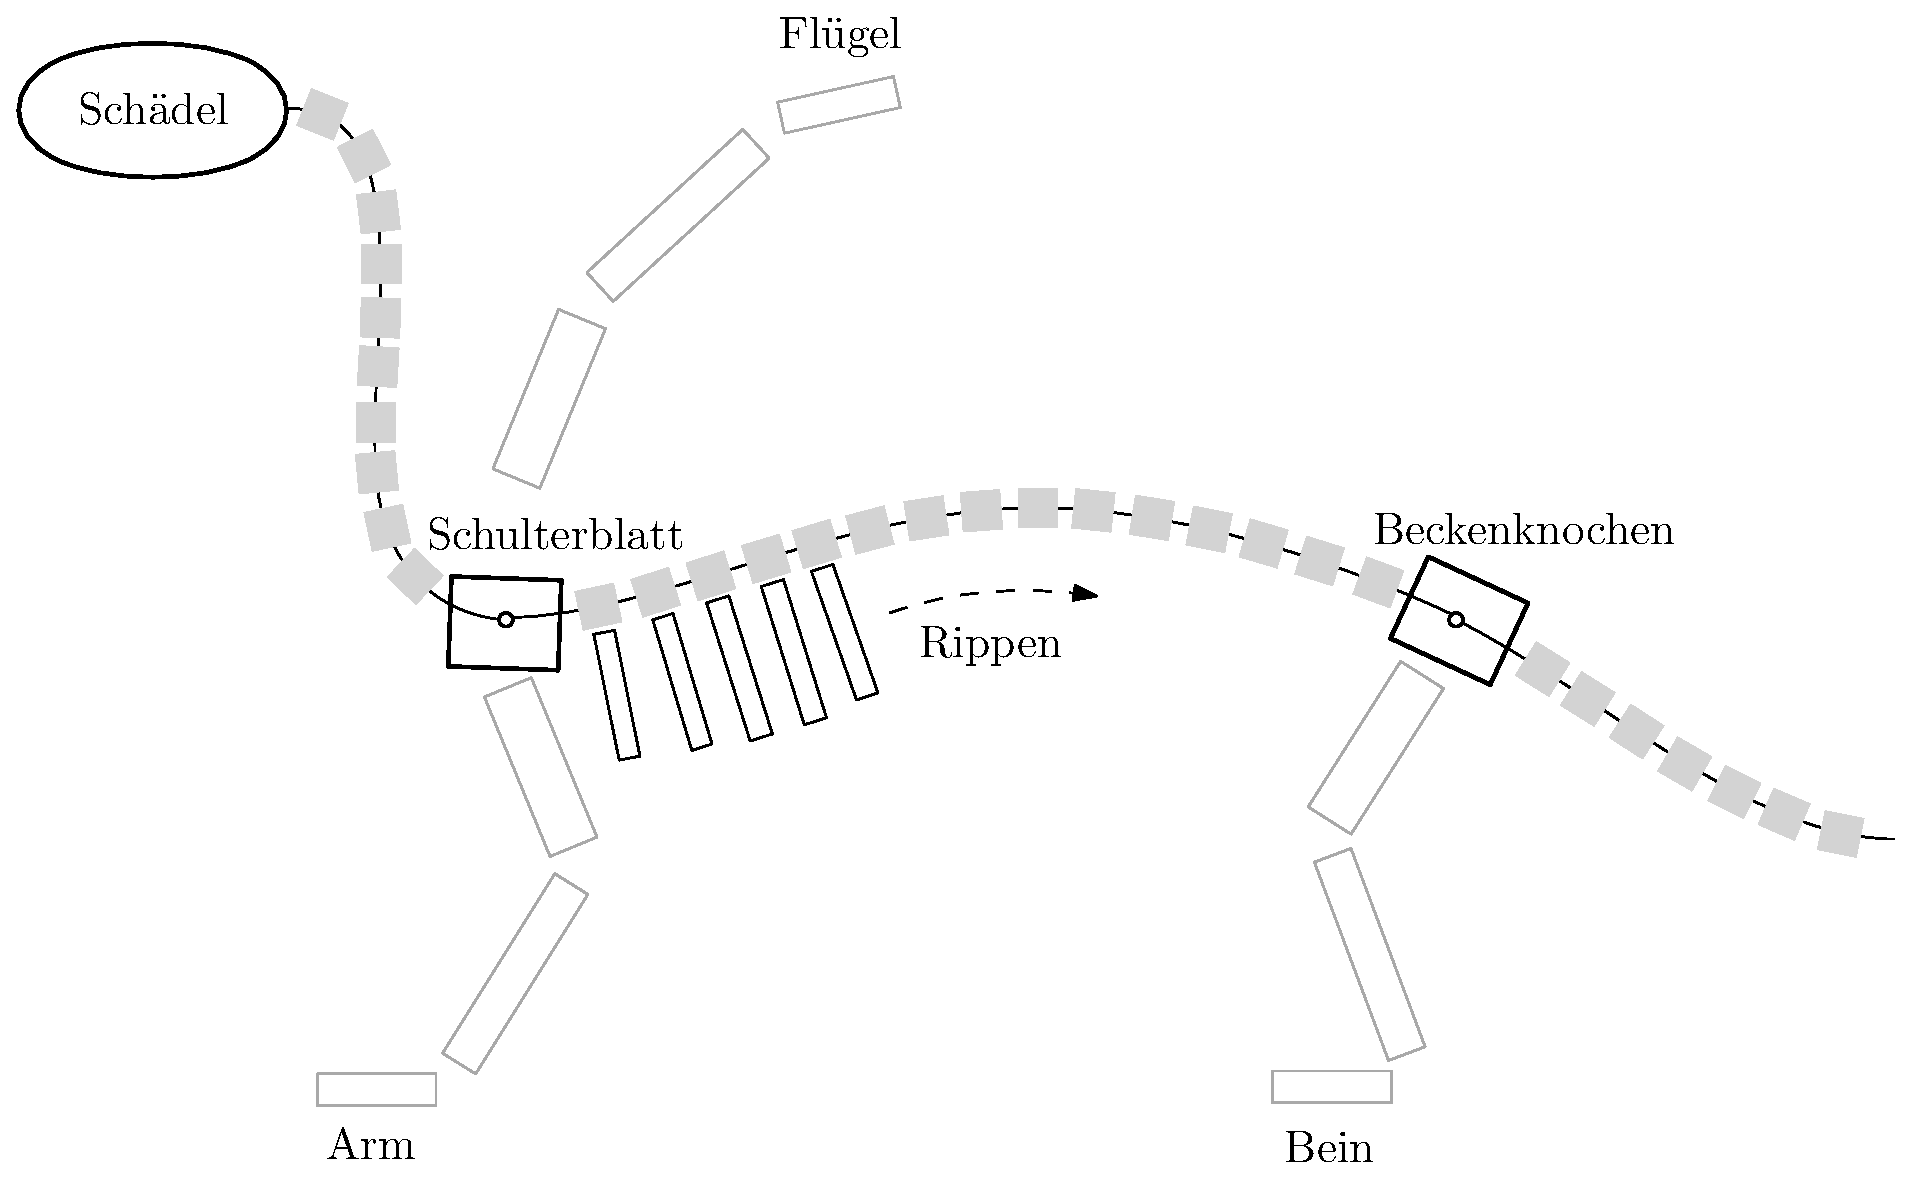
\includegraphics[width=\textwidth]{graphics/skeletonPlan}
 \caption{Verallgemeinerter und abstrahierter Bauplan eines Wirbeltierskeletts. Es sind maximal zwei Extremitätenpaare erlaubt, jeweils eines an jedem Extremitätengürtel. Rippen und Hals- und Schwanzwirbelsäule sind optional. Die Anzahl der Wirbel und Rippen variiert je nach Tier.}
 \label{bauplan_skelett}
\end{figure}


%-----------------------------------------------------
\section{Von Groß und Klein}
\label{bigAndSmall}

Dieser Abschnitt widmet sich der Frage nach Unterschieden und Gemeinsamkeiten von großen und kleinen Wirbeltieren. Kann man Wirbeltiere und ihre Skelette einfach vergrößern und verkleinern? Oder sind sie besonders an ihre Größe angepasst? Unterscheidet sich das Skelett einer Maus wesentlich von dem eines Elefanten?

% Extrema
Zunächst ein kurzer Überblick über die Dimensionen, in denen man sich hier bewegt:\\
Das größte und schwerste Wirbeltier ist der Blauwal, er kann bis zu $120$ Tonnen wiegen (siehe \ref{appendix_pca_weight}). Das aktuell kleinste bekannte Wirbeltier, mit einer Länge von $7$ bis $8$mm, ist der Frosch \emph{Paedophryne amauensis} \cite{smallestVertebrate}. Größe und Gewicht von Wirbeltieren kann also erheblich variieren.

% Probleme bei Skalierung
Wenn eine Tierart im Laufe der Evolution wächst, so ändert sich die Größe gleichmäßig. Dieses Wachstum ist aber begrenzt. Der Grund dafür ist, dass die Oberfläche nicht proportional mit dem Volumen mitwächst. Beispielsweise produziert ein Säugetier Wärme proportional zu seinem Volumen. Es kann aber nur Wärme proportional zu seiner Oberfläche abgeben. Dadurch haben große Säugetiere eher Probleme Wärme abzugeben und kleine warm zu bleiben.
Ein ähnliches Problem tritt bei Knochen auf. Die Last, die ein Knochen tragen kann, ist ungefähr proportional zu seiner Querschnittsfläche. Das Skelett muss aber das komplette Gewicht des Körpers tragen, was wiederum proportional zum Volumen ist.
% Lösungen für Skalierungen
Aus diesem Grund müssten die Knochen großer Tiere eigentlich überproportional vergrößert sein. Das ist jedoch nicht unbedingt der Fall. Das Problem an dicken Knochen ist, dass sie den Bewegungsradius, \zb der Extremitäten, stark einschränken. Deshalb passen viele Tiere stattdessen ihre Körperhaltung und Aktivität an, um Spitzenkräfte, wie Stöße oder Oszillationen, auf ihre Knochen zu vermeiden. Deshalb wirken große Tiere auch eher "`behäbiger"' als kleine. (\cite{Vergleichende_Anatomie}, Kapitel 23)

Sehr große und sehr kleine Wirbeltiere können also nicht über einfaches Skalieren ineinander überführt werden. Dennoch ähneln sich ihre Skelette sehr.


%-------------------
\section{Mythologie}
\label{biology_mythology}

In diesem Abschnitt wird ein kurzer Blick über die Biologie hinaus, auf fantastische Tiere aus der Mythologie geworfen. 
Ein Algorithmus, der wirbeltierähnliche Skelette erzeugt, bewegt sich ja schon über die Grenzen der Biologie hinaus. Da ist es nur ein kleiner Schritt auch fiktive Wirbeltiere mit zusätzlichen Gliedmaßen zu erzeugen.
Einen guten Überblick über solche Tiere, nicht nur aus der Mythologie sondern auch aus aktuellerer Literatur, Filmen oder Spielen, gibt die Webseite \cite{vertebrateExtraLimbs}.

Hier sollen drei Beispiele hervorgehoben werden, die jeweils charakteristische Merkmale besitzen. Sie stammen aus der Mythologie und bilden oft auch die Grundlage für andere fiktive Wirbeltiere.

\emph{Zentauren} haben einen Pferdekörper, aber statt eines Halses setzt ein menschlicher Oberkörper auf dem Schultergürtel auf \cite{centaurs}. Sie haben also zwei Schultergürtel. 
%\todo{Paper zu Mischwesen zitieren?}

Der \emph{Pegasus} hat ebenfalls den Körper eines Pferdes, aber auch Flügel, die zusätzlich zu den Vorderbeinen am Schultergürtel ansetzen \cite{pegasus}. Es ist also "`möglich"' an einem Extremitätengürtel zwei Paare von Extremitäten ansetzen zu lassen.

\emph{Asiatische Drachen} haben einen langen, schlangenartigen Körper mit oft mehr als vier Beinen. Sie können als Inspiration für Tiere dienen, die mehr als nur zwei Extreimtätengürtel entlang des Rückens besitzen.


%-------------------
%-------------------
\chapter{Grundlagen}
\label{chapter:basics}
%  Vergleich von Techniken, was gibt es alles, was wurde am Ende verwendet und warum

Dieses Kapitel stellt diejenigen Techniken und Ansätze vor, die zum Verständnis dieser Arbeit nötig \bzw hilfreich sind. Zunächst wird die prozedurale Generierung (\ref{procedural_generation}) vorgestellt. Dann geht es um die Animation von 3D-Modellen von Figuren (\ref{character_animation}), da dies ein möglicher Schritt ist, wie die erzeugten Skelette weiterverarbeitet werden können.
Ein kurzer Abschnitt widmet sich der inversen Kinematik (\ref{IK}), da ihre Konzepte zum Verständnis hilfreich sind. Sie kommt aber im Algorithmus nicht zur Anwendung. Wichtige Konzepte, die im Algorithmus verwendet werden, sind Grammatiken (\ref{grammars}) und \emph{Principal Component Analysis} (PCA) (\ref{PCA}). Um die Beispiele, auf denen eine PCA durchgeführt werden soll, zu untersuchen, werden Quantil-Quantil-Diagramme (\ref{qqdiagrams}) eingesetzt.
Der letzte Abschnitt widmet sich genetischen Algorithmen (\ref{genetic_algorithms}), da sie nah am Themengebiet dieser Arbeit liegen und in alternativen Ansätzen verwendet werden könnten.


%--------------------------------
\section{Prozedurale Generierung}
\label{procedural_generation}

Werden Inhalte, wie Texturen oder 3D-Objekte, generiert, ohne dass diese vor der Ausführung des Algorithmus festgelegt wurden, so wird dies als prozedurale Generierung (PG) bezeichnet.
Ursprünglich wurde PG verwendet, weil der Speicherplatz auf Computern sehr begrenzt war. Große 3D-Landschaften oder andere vorgefertigte künstlerische Werke konnten nicht gespeichert werden.\\
Die Demoszene treibt PG ins Extreme. Sie entstand in den 1980er Jahren und zeigt mit künstlerischen Inhalten, dass beeindruckende Ergebnisse trotz stark limitiertem Speicherplatz möglich sind \bzw wie das volle Potential von Computerhardware ausgeschöpft werden kann \cite{DemoScene}. 

Auf heutigen Rechnern ist der Speicherplatz nicht mehr so begrenzt und es kann viel Inhalt, \zb für PC-Spiele, von KünstlerInnen vorgefertigt werden. Trotzdem behält PG ihre Daseinsberechtigung, da der Entwurf komplexer Inhalte, wie beispielsweise Landschaften mit viel Vegetation, aufwändig ist und viel Zeit benötigt. Hier können wieder Algorithmen aus der PG eingesetzt werden um Zeit und Arbeit zu sparen. Sie können sowohl fertige 3D-Modelle generieren, als auch Inspiration und Hilfe für KünstlerInnen sein. \emph{SpeedTree}~\cite{SpeedTree} ist ein Beispiel für Software, die für die Generierung von Vegetation verwendet wird. Sie unterstützt und beschleunigt die Erstellung von Szenen mit viel Vegetation. \cite{PCGSurvey_videoGames}

Dinge, die prozedural generiert werden können, sind \zb Landschaften, Straßennetze, Gebäude, Menschen, Tiere oder auch Geschichten \cite{PCGSurvey}. 
Oft werden für ihre Generierung Rauschfunktionen nach Perlin (oder auch Perlin-Noise) \cite{perlinNoise} verwendet. Klassische Anwendungsgebiete für Perlin-Noise sind \zb die Generierung von Texturen, Höhenfeldern oder Volumina, wie Feuer oder Wolken. Zur Generierung von Lebewesen oder deren Skeletten ist Perlin-Noise nicht geeignet, da diese zu viele festgelegte Strukturen haben.\\
Humanoide Charaktere für Computerspiele werden \zb in der Masterarbeit \cite{ProceduralCharacterGeneration} erzeugt und die Zusammenstellung \cite{PCGSurvey_videoGames} untersucht die PG von Wesen, die Videospiele bevölkern. Obwohl in \cite{PCGSurvey_videoGames} einige Arbeiten genannt werden, die sich mit der Generierung solcher Wesen beschäftigen, wird auch festgestellt, dass dieser Themenbereich noch wenig erforscht ist. \\
Ein Beispiel, das erst nach Erscheinen dieser Zusammenstellung auf den Markt gekommen ist, ist das Computerspiel "`No Man's Sky"' \cite{NoMansSky}. Darin gibt es viele prozedural generierte fantastische Tiere. Zur Generierung dieser Tiere wird zunächst prozedural ein 3D-Modell generiert, in welches anschließend ein Rig eingepasst wird \cite{NoMansSkyDevelopment}.
Die dort verwendeten Rigs sind keine wirklichkeitsgetreuen Skelette, sondern werden nur für die Animation verwendet (siehe Abschnitt \ref{character_animation}).


%------------------------------
\section{Animation von Figuren}
\label{character_animation}

Um Figuren für Computerspiele oder Filme zu animieren, ist außer dem 3D-Modell ein Skelett \bzw Rig nötig. Dieses Rig ist oft sehr abstrakt und hat wenig mit lebensechten Skeletten zu tun. Es gibt eine Baumstruktur auf den Einzelteilen der Figur vor. Diese Baumstruktur ist für viele Algorithmen, die zur Animation verwendet werden, essentiell, \zb für inverse Kinematik (siehe Abschnitt \ref{IK}). Als Wurzel für das Rig wird meist ein Knochen in der Nähe des Schwerpunkts der Figur verwendet. Das ist bei humanoiden Figuren die Hüfte.\\
Weit verbreitete Editoren für Animation, Modellierung, Simulation und Rendering sind Maya \cite{Maya} und 3ds Max \cite{3dsMax}. Auch hier werden solche Rigs verwendet. 3ds Max stellt \zb in einer Komponente namens Biped vorgefertigte Rigs für humanoide Figuren zur Verfügung, die einfach in schon existierende 3D-Modelle eingefügt werden können \cite{3dsMaxBiped}.

Animationen werden dann mit Hilfe sogenannter Keyframes erzeugt. Keyframes sind Positionen, die die Figur im Laufe der Bewegung einnehmen soll. Interpolation zwischen den einzelnen Keyframes ergibt dann eine flüssige Bewegung. \cite[Kapitel 3]{sporeanim}\\
Im Computerspiel Spore \cite{Spore} werden sogar zur Laufzeit Animationen für Figuren erzeugt, deren Aufbau vorher noch nicht bekannt war. Dazu werden vorher abstrakte Animationen, unabhängig vom Aufbau der speziellen Figur, erstellt. Diese werden dann zur Laufzeit auf die konkreten Figuren angewandt. \cite{sporeanim}

Um besonders lebensecht wirkende Tiere zu erzeugen, ist es nötig den Aufbau des entsprechenden Tieres möglichst wirklichkeitsgetreu zu modellieren. Dazu sind Modelle für Skelett, Muskeln und Haut nötig. Solche Modelle lassen sich beispielsweise mit dem Maya-Plugin Ziva \cite{Ziva} gestalten.


% \begin{itemize}
%  \item Featherstone Algorithmus
%  \item skeleton-based design tool (Yamamoto et al 2011): rudimentäres Skelett/Rig für schnelle Produktion und leichte Änderung an Charakteren
%         \url{https://dl.acm.org/doi/10.1145/2073304.2073316}, \url{https://www.youtube.com/watch?v=yhq1aUp8QLY}
% \end{itemize}


%--------------------------
\section{Inverse Kinematik}
\label{IK}

Inverse Kinematik wird beispielsweise in der Robotik zur Bewegung von Roboterarmen verwendet. Gegeben ist eine Kette von Gelenken, die über starre Verbindungsteile miteinander verbunden sind. Für ein oder mehrere Punkte dieser Kette können Zielpunkte im Raum angegeben werden. Das Ziel ist es dann eine Konfiguration der Gelenke zu berechnen, so dass alle Punkte ihr Ziel erreichen.

Es gibt viele verschiedene Methoden Probleme aus der inversen Kinematik zu lösen. Diese finden jeweils in Abhängigkeit von der konkreten Problemstellung ihre Anwendung. Beispielsweise wird in \cite{IKLegs} die Animation von Beinen untersucht. Ein Überblick über die verschiedenen Techniken ist in der Zusammenstellung \cite{IKSurvey} zu finden.

% IK die gelernte Posen bevorzugt: style-based inverse kinematics (\url{https://grail.cs.washington.edu/projects/styleik/})


%-------------------------------------
\section{Principal Component Analysis}
\label{PCA}
 
 % Ziel
 \emph{Principal Component Analysis} (PCA) oder auch Hauptkomponentenanalyse \cite{PCA} wird meist mit dem Ziel angewendet die Dimensionalität einer Menge von Datenpunkten zu verringern, dabei aber möglichst wenig Information zu verlieren.
 Beispielsweise wird sie im Zusammenhang mit 3D-Modellen von Gesichtern \cite{PCA_faces} oder 3D-Modellen von menschlichen Körpern \cite{PCA_bodies} eingesetzt. Auch im Zusammenhang mit prozeduraler Generierung wird PCA oft verwendet, \zb zur Generierung von humanoiden Charakteren für Videospiele~\cite{ProceduralCharacterGeneration} oder Texturen für Gesichter \cite{GeneratingFacialTextures}.
 
 Als Ausgangspunkt für eine PCA dient eine Menge von Datenpunkten (oder Beispielen) $D$ im $n$-dimensionalen Raum. Voraussetzung ist, dass die Punkte in jeder Dimension normalverteilt sind. 
 Die Datenpunkte $D$ sind dann nach einer $n$-dimensionalen Normalverteilung verteilt. Betrachtet man nun die Wahrscheinlichkeitsdichte dieser Normalverteilung, so bilden alle Punkte, bei denen die Dichte einen Wert größer als $\epsilon$ annimmt, das Innere eines $(n-1)$-dimensionalen Hyperellipsoids. In diesem Volumen liegen die meisten der Datenpunkte $D$. Ihr Mittelwert bildet den Mittelpunkt.
 
 Nun ist das Ziel herauszufinden wo die Achsen des Hyperellipsoids liegen. Betrachtet man die Komponenten der Datenpunkte $D$ in den Richtungen der Achsen, so sind diese wiederum normalverteilt und die Verteilungen sind jeweils unabhängig voneinander.
 Um die Achsen des Hyperellipsoids zu berechnen, wird zunächst die Kovarianzmatrix der Datenpunkte $D$ aufgestellt und diese dann diagonalisiert. Die Spalten der damit berechneten Basiswechselmatrix bilden eine Orthonormalbasis $\mathcal{B}$ aus Eigenvektoren. Auf der Diagonalen der diagonalisierten Kovarianzmatrix stehen die Eigenwerte. Diese sind immer $\geq 0$.
 Die Eigenvektoren sind die Achsen des Hyperellipsoids und die Eigenwerte geben die Varianz der Normalverteilung entlang der Achsen an.
 
 
 Jetzt können die Datenpunkte $D$ vom Eingabekoordinatensystem in dasjenige Koordinatensystem transformiert werden, das von den Achsen des Hyperellipsoids aufgespannt wird. Dazu stellt man die Punkte als Linearkombinationen der Eigenvektoren dar.\\
 Die Vektoren der Basis $\mathcal{B}$ werden nun absteigend nach der Größe der dazugehörigen Eigenwerte sortiert. Diese Basis wird im Folgenden \emph{PCA-Basis} genannt. Der $i$-te Vektor der PCA-Basis wird als \emph{\mbox{$i$-ter} Eigenvektor} bezeichnet. Die ersten $m$ Eigenvektoren sind die Hauptkomponenten oder "`principal components"'.
 Um nun die Dimensionalität der Eingabedaten zu reduzieren, werden sie auf den Raum projiziert, der von den Hauptkomponenten aufgespannt wird. Je weniger Streuung die Datenpunkte auf denjenigen Achsen aufweisen, die weggelassen werden, desto weniger Information wird verworfen.
 
 Will man einen zufälligen Datenpunkt erzeugen, der die gleiche Verteilung aufweist, wie die Eingabebeispiele, so funktioniert das im transformierten Koordinatensystem sehr gut. Da die einzelnen Dimensionen unabhängig voneinander sind, kann einfach für jede Dimension eine normalverteilte Zufallszahl mit entsprechender Varianz generiert werden.
 
 
%---------------------------------- 
\section{Quantil-Quantil-Diagramme} 
\label{qqdiagrams}

Quantil-Quantil-Diagramme sind eine grafische Methode um zu testen, ob eine Stichprobe einer bestimmten Verteilung unterliegt. \\
Seien $x_1, x_2,\dots, x_n$ die Elemente einer Stichprobe und $F$ die Verteilungsfunktion derjenigen Verteilung, gegen die getestet werden soll. Die Verteilungsfunktion gibt für einen Wert~$x$ an, wie groß die Wahrscheinlichkeit ist, dass eine nach $F$ verteilte Zufallsvariable einen Wert $\leq x$ annimmt.\\
Nun werden die empirischen Quantile der Stichprobe mit den entsprechenden Quantilen von $F$ verglichen. Dazu wird die Stichprobe aufsteigend sortiert, was $x_{(1)}, x_{(2)},\dots, x_{(n)}$ ergibt. 
Das empirische $\frac{i}{n}$-Quantil der Stichprobe ist $x_{(i)}$, da $i$ Werte $\leq x_{(i)}$ beobachtet wurden. Die inverse Verteilungsfunktion gibt für einen Wert $y$ den kleinsten Wert $x$ an, für den gilt, dass $F(x) > y$ ist, also das $y$-Quantil. Das $\frac{i}{n}$-Quantil von $F$ ist also $F^{-1}\left(\frac{i}{n}\right)$.

Trägt man nun die sortierte Stichprobe gegen die entsprechenden Quantile in ein Diagramm ab, und die angenommene Verteilung ist korrekt, so liegen die Punkte annähernd auf einer Geraden mit Steigung $1$ durch den Ursprung. \cite[Kapitel 1 und 2]{QQPlots}

Den Werten $x_{(i)}$ einfach das $\frac{i}{n}$-Quantil zuzuordnen ist aber insofern schwierig, als dass es suggeriert, dass alle Werte, die mit der angenommenen Verteilung generiert werden, kleiner als $x_{(n)}$ sind. Deshalb gibt es verschiedene andere Möglichkeiten die Quantile zuzuordnen. Sie liefern aber für $n \rightarrow \infty$ alle das gleiche Ergebnis. Sogenannte "`Rankit Plots"' verwenden folgende Zuordnung:
\[ x_{(i)} \approx F^{-1}\left(\frac{i - 0{,}5}{n}\right). \]
Diese Zuordnung wird auch in dieser Arbeit verwendet.


%--------------------
\section{Grammatiken}
\label{grammars}

Eine \emph{Grammatik} ist ein Tupel $G = (\Sigma, N, S, P)$ mit 
\begin{itemize}
 \item dem endlichen Alphabet $\Sigma$ der Terminalsymbole
 \item dem endlichen Alphabet $N$ der Nichtterminalsymbole
 \item dem Startsymbol $S \in N$ und
 \item der Menge von Produktionen $P \subseteq (N \cup \Sigma)^* N (N \cup \Sigma)^* \rightarrow (N \cup \Sigma)^*$
\end{itemize}

Eine Teilmenge der Grammatiken bilden die \emph{kontextsensitiven} Grammatiken. Ihre Produktionen haben die Form
\[\alpha A \beta \rightarrow \alpha \gamma \beta \text{ oder } S \rightarrow \epsilon\] \[\text{ mit } A \in N,~ \alpha, \beta, \gamma \in ((N \setminus \{ S \}) \cup \Sigma)^*,~ \gamma \neq \epsilon \text.\]
Dabei ist $\epsilon$ das leere Wort.

Wiederum eine Teilmenge davon bilden die \emph{kontextfreien} Grammatiken mit Produktionen der Form 
\[A \rightarrow w \text{ mit } A \in N \text{ und } w \in (N \cup \Sigma)^*.\] \cite[Abschnitte 1.4 und 1.5]{FormalLanguageTheory}

\emph{L-Systeme} oder Lindenmayer-Systeme sind spezielle Grammatiken. Sie wurden 1968 von dem Biologen Aristid Lindenmayer vorgestellt, mit dem Zweck das Wachstum vielzelliger Lebewesen zu modellieren. Im Unterschied zu Grammatiken, bei denen Produktionen einzeln nacheinander angewendet werden, werden bei L-Systemen alle Symbole gleichzeitig ersetzt. Dies soll modellieren, dass viele Zellteilungen zur gleichen Zeit stattfinden können.\\
Auch hier gibt es wieder verschiedene Teilmengen wie \zb kontextfreie und kontextsensitive L-Systeme. Kontextfreie L-Systeme sind aber keine Teilmenge kontextfreier Grammatiken. Es gibt Sprachen, die von kontextfreien L-Systemen, aber nicht von kontextfreien Grammatiken erzeugt werden können und anders herum \cite[Abbildung 1.2]{AlgorithmicBeautyOfPlants}.\\
Oft werden L-Systeme verwendet um das Wachstum von Pflanzen zu modellieren. Es gibt aber auch andere Anwendungsbeispiele, wie \zb die Generierung von Städten \cite{cityGeneration}. 

Bei Pflanzen treten oft Verzweigungen auf. Um diese zu modellieren, werden in L-Systemen Klammerstrukturen verwendet. Das Teilwort innerhalb einer Klammer repräsentiert einen "`Ast"', der wiederum in sich verzweigt sein kann.
Wenn zwei Symbole direkt aufeinander folgen, so bedeutet das, dass das linke Element das Elternelement des rechten ist. Kommt in einem Wort $A(BC)D$ mit $A, B, C, D \in \Sigma \cup N$ ein Klammerausdruck vor, so bedeutet dies, dass $A$ sowohl das Elternelement von $B$ als auch von $D$ ist. Das Elternelement von $C$ ist $B$. Es können auch Mehrfachverzweigungen auftreten. In $A(B)(C)D$, was gleichbedeutend ist zu $A(B)(C)(D)$, ist $A$ das Elternelement von $B, C$ und $D$. Eine Visualisierung der beiden Beispiele ist in Abbildung \ref{branching_examples} zu finden. \cite[Kapitel 1]{AlgorithmicBeautyOfPlants}

\begin{figure}
 \centering
 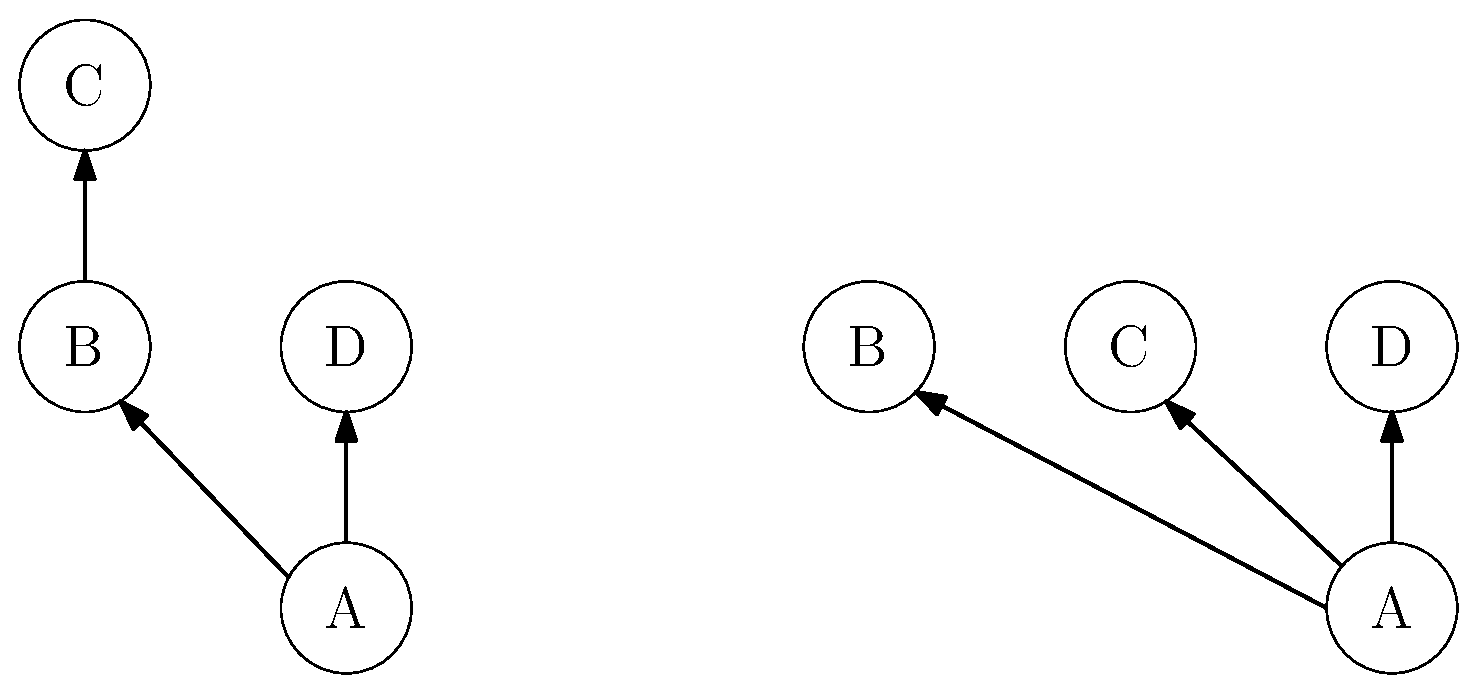
\includegraphics[width=0.6\textwidth]{graphics/branchingExamples}
 \caption{Visualisierung der Beispiele für Klammerausdrücke, links der \mbox{Ausdruck $A(BC)D$}, rechts $A(B)(C)D$.}
 \label{branching_examples}
\end{figure}


%-------------------------------
\section{Genetische Algorithmen}
\label{genetic_algorithms}

Ein sehr bekannter Zweig der evolutionären Algorithmen sind die genetischen Algorithmen.
Die Grundprinzipien, die von genetischen Algorithmen verwendet werden, sind von Evolution und natürlicher Auslese inspiriert. Im einfachsten Fall sind eine Fitnessfunktion und eine Menge von Individuen (oder eine Population) gegeben, die durch "`Gene"' kodiert sind. Die Fitnessfunktion bewertet die Individuen. Das Ziel ist Individuen zu entwickeln, die möglichst gut bewertet werden. 
Dazu werden aus der aktuellen Population zufällig, aber nach Fitness priorisiert, Individuen ausgewählt. Diese produzieren dann "`Nachkommen"' indem sie ihre Gene nach einer bestimmten Vorschrift vermischen.
Diese "`Nachkommen"' bilden dann eine neue Population, die wiederum anhand der Fitnessfunktion bewertet wird. Damit startet eine neue Iteration.
Dies wird so lange durchgeführt bis ein Individuum gefunden wurde, das die Fitnessfunktion gut genug erfüllt. \cite{Holland} \cite[Abschnitt 1.3.1]{EvolutionaryDesign_Introduction}\\
In interaktiven Versionen evolutionärer Algorithmen können sogar Benutzer die Fitnessfunktion ersetzen, indem sie selbst die erzeugten Individuen bewerten. \cite{InteractiveEvolutionaryComputation}

In der Masterarbeit \cite{JonHudson} werden 3D-Modelle von Lebewesen und ein passendes Rig (siehe Abschnitt \ref{character_animation}) mit Hilfe von genetischen Algorithmen generiert. Das Augenmerk liegt dort, im Gegensatz zu dieser Arbeit, aber nicht auf realistischen Tieren oder realistischen Skeletten.

%---------------------------
%---------------------------
\chapter{Bisherige Arbeiten}

\begin{itemize}
 \item Aufbau des Skeletts mit Aufbau von Skeletten, die für Animation verwendet werden, vergleichen (realistischer, ...)
\end{itemize}



%-------------
\section{Ziva}

\begin{itemize}
 \item Ziva VFX Maya Plugin zur Erstellung von Charakteren und Simulation von biomechanischen Bewegungen \url{https://zivadynamics.com/}
 \item Charaktererstellung in Ziva beginnt mit der Modellierung des Skeletts. Knochen mit Animationen werden als Alembic-Datei gespeichert und dann in "`Ziva-Knochen"' konvertiert. \url{https://discover.therookies.co/2019/06/01/vfx-in-9-steps/}
\end{itemize}

%---------------------------
\section{ZSpheres in Zbrush}

\begin{itemize}
 \item \url{http://docs.pixologic.com/user-guide/3d-modeling/modeling-basics/creating-meshes/zspheres/},\\ Beispielvideo: \url{https://www.youtube.com/watch?v=Wl0XK6ggUOA}
 \item Möglichkeit ein "`Skelett"' aus Kugeln zu erstellen. Definiert aber eher die grobe Außenhaut mit Zusatzinformationen dazu wo die Gelenke sind.
\end{itemize}

%----------------------
\section{3DS MAX Biped}

\begin{itemize}
 \item \url{https://knowledge.autodesk.com/support/3ds-max/learn-explore/caas/CloudHelp/cloudhelp/2019/ENU/3DSMax-Character-Animation/files/GUID-2F6BC5D1-DD45-4C2E-AC3A-D8C6E0F5DEB1-htm.html}
 \item Möglichkeit Skelett in einen fertig modellierten Körper einzupassen. 
 \item Skelette sind schon vorgefertigt.
 \item v.a. für menschliche Skelette, aber auch (limitiert) anpassbar auf Tiere
\end{itemize}

%---------------------------------
\section{Forensik und Archäologie}

\begin{itemize}
 \item forensische Gesichstrekonstruktion ist spezialisiert auf Menschen und verwendet Zusatzinformationen wie Stockfotos von Gesichtsmerkmalen (\url{https://en.wikipedia.org/wiki/Forensic_facial_reconstruction})
 \item Rekonstruktion von Tieren in der Archäologie anhand des Skeletts v.a. durch Künstler (?)
\end{itemize}


%----------------------
\section{No Man's Sky}

\begin{itemize}
 \item Webseite \cite{NoMansSky}
 \item "`For creatures, basic templates of creatures that exist on the Earth were created and then manipulated by the system, changing everything from height, weight, bone density, voice pitch, what it eats, and its behaviors, even creating variation within the species."' (\url{https://nomanssky.fandom.com/wiki/Biology})
 \item "`Creatures were often generated by mixing and matching random parts from a library, and then adjusting the underlying skeleton so that the creature appeared realistic; a creature with a tiny body could not support a giant head, for example."' (\url{https://en.wikipedia.org/wiki/Development_of_No_Man\%27s_Sky})
 \item Zunächst Generierung von äußerem 3D-Modell, dann Anpassung der Knochen.
\end{itemize}

%---------------------
\section{Avatar movie}

\begin{itemize}
 \item Direhorse (Schreckenspferd) hat sechs Beine (vier vorne, zwei hinten).\\
 Bilder: \url{https://james-camerons-avatar.fandom.com/wiki/Gallery:_Pandoran_Creatures?file=Muscle.jpg}, \url{https://james-camerons-avatar.fandom.com/wiki/Gallery:_Pandoran_Creatures?file=Pandora_ROVR_Direhorse.png}
 \item Prolemuris hat Arme, mit einem Oberarm, aber zwei Unterarmen.\\
 Bild: \url{https://james-camerons-avatar.fandom.com/wiki/Gallery:_Pandoran_Creatures}
\end{itemize}


%-------------------
\section{Mythologie}

\begin{itemize}
 \item Zentauren haben Körper wie ein Pferd, aber statt einem Hals setzt ein menschlicher Oberkörper auf Schultergürtel auf.\\
 \url{https://tvtropes.org/pmwiki/pmwiki.php/Main/OurCentaursAreDifferent?from=Main.CentauroidForm}
 \item Pegasus hat den Körper eines Pferdes + Flügel, die zusätzlich zu den Vorderbeinen an Schultergürtel ansetzen\\
 \url{https://tvtropes.org/pmwiki/pmwiki.php/Main/Pegasus}
\end{itemize}

%-----------------------------------
%-----------------------------------
\chapter{Erste Ansätze und Probleme}

%------------------------------------
\section{Bestandteile eines Skeletts}

Ein Skelett besteht aus Knochen und Gelenken. Zwei Knochen sind jeweils durch ein Gelenk miteinander verbunden. Im Folgenden werden beide Bestandteile jeweils genauer beschrieben.

% Knochen
Jeder Knochen hat sein eigenes lokales Koordinatensystem und wird zunächst als Quader dargestellt. Der Ursprung des Koordinatensystems befindet sich in einer Ecke des Quaders.
Informationen, die für die Darstellung eines Knochens erforderlich sind, sind also
seine Ausdehnung in alle drei Raumrichtungen (die Kantenlängen des Quaders) und die Position und Orientierung des Ursprungs im globalen Koordinatensystem.

% Hierarchie
Die Knochen sollten eine Hierarche (einen Baum) bilden, da das von Algorithmen für Animationen so erwartet wird. \todo{Verweis auf previous work, wenn ausgearbeitet}
Es gibt also einen Knochen, der das oberste Element in der Hierarchie ist \bzw der die Wurzel des Baums bildet. Dieser wird im Folgenden als \emph{Wurzelknochen} bezeichnet. Liegt Knochen $B$ in der Hierarchie direkt unter Knochen $A$, so ist $A$ der \emph{Elternknochen} von $B$ und $B$ ein \emph{Kindknochen} von $A$.

% Transformationsmatrizen
Es ist also sinnvoll für jeden Knochen nicht die Position im globalen Koordinatensystem anzugeben, sondern seine Position im Koordinatensystem des Elternknochens. Verfolgt man den Pfad von einem Knochen zurück zum Wurzelknochen, so kann die Position im globalen Koordinatensystem trotzdem ausgerechnet werden.\\
Für die Darstellung werden Transformationsmatrizen mit homogenen Koordinaten verwendet. Genauere Informationen zu diesen Transformationsmatrizen und wie sie in verschiedenen Situationen berechnet werden können sind in Absatz \ref{implementation_detail_matrices} zu finden.

% Wurzel
Für die Wahl des Wurzelknochens bietet sich ein Knochen in der Nähe des Schwerpunkts an. Oft wird hierfür die Hüfte verwendet. \todo{Beispiel/Quelle}
Da aber nicht jedes Wirbeltier eine Hüfte besitzt und es für die Generierung einfach ist, wird als Wurzelknochen ein Knochen ohne Ausdehnung in der Mitte der Rückenwirbelsäule verwendet.


% Gelenke
Ein Gelenk ist, wie auch in der Natur, ein Verbindungsstück zwischen zwei Knochen. Es legt fest wie die beiden Knochen sich relativ zueinander bewegen können. Im Gegensatz zu echten Gelenken haben Gelenke hier aber keine Ausdehnung. Sie werden am Ende im 3D-Modell nicht dargestellt.\\
Ein Gelenk wird im Koordinatensystem des Elternknochens dargestellt. Es wird beschrieben durch seinen Abstand zum Ursprung des Elternkoordinatensystems und Bewegungseinschränkungen für den Kindknochen. Ein Gelenk kann null bis zwei Freiheitsgrade haben. Bei einem Winkel von $0^\circ$ hat das Kindelement die gleiche Ausrichtung wie das Elternelement.
\todo{Schaubilder für verschiedene Gelenkarten}

% Berechnung Transformationsmatrix des Kindelements
Ist ein Elternknochen mit einem Gelenk in einer bestimmten Ausrichtung gegeben, so lässt sich daraus die Transformationsmatrix des Kindelements berechnen.


%-----------------------------
\section{Aufbau als Grammatik}

\begin{itemize}
  \item Aufbau als Grammatik (am Ende aber für jedes Nichtterminal genau eine Regel)
  \item Aufbau der (Nicht)terminale als Baum, nur Terminale können Kinder haben, Reihenfolge der Anwendung der Regeln sollte beliebig sein
  \item Wachstum unter Berücksichtigung verschiedener Randbedingungen wie Bodenposition, Anzahl Extremitäten etc.\ Bounding Box für Nichtterminale ist dafür aber nicht nötig.
  \item Symmetrie der Skelette (spiegle Elemente zum Schluss)
  \item Repräsentation des Zustands als Hierarchie von einzelnen Komponenten (terminale sowie nichtterminale)
 \end{itemize}
 
 \begin{itemize}
  \item Iterative Erzeugung eines Skeletts durch eine probabilistische kontextfreie (?) Grammatik, die so erweitert ist, dass sie nicht ein einfaches Wort erzeugt, sondern einen Baum von Zeichen (nötig für Extremitäten). Verwendung von paramterischen L-Systemen \cite{Paramteric_L-Systems} könnte sinnvoll sein.
  
  \item Regeln sind nicht wirklich eine Grammatik, da fast jedes nichtterminale Literal nur einmal vorkommt, wenn es für jedes Körperteil andere Regeln gibt. Oder ist es möglich so zu abstrahieren, dass z.B. Arme und Beine den gleichen/ähnlichen Regeln unterliegen? Ist das sinnvoll? \todo{Abstraktionsgrad, Art der Regeln}\\
  \todo{Graphen zur Visualisierung der Regeln einfügen}
  Außerdem ist das Skelett nicht unbedingt zusammenhängend (siehe Biologie). $\rightarrow$ Darauf achten, dass das nicht von Algorithmus verlangt wird
  
  \item Brustbein sorgt dafür, dass Skelett nicht mehr baumartig $\rightarrow$ erstmal weglassen, ist wahrscheinlich auch nicht unglaublich relevant
  
  \item Kindelement erst erzeugen, wenn Elternelement terminal ist und Gelenk hat.
 \end{itemize}

 

%---------------------
\section{Pose des Skeletts}

Ein Skelett ist nicht nur eine Hierarchie von Knochen, sondern wirkt auch wesentlich durch seine Pose. Das Ziel sollte also sein das Skelett in einer natürlich wirkenden Pose darzustellen, eine Pose, die das dargestellte Tier auch einnehmen würde.

% erster Ansatz: Drehmomente
Ein erster Ansatz könnte sein in jedem Schritt auszurechnen, ob das Skelett ausbalanciert ist. Dazu benötigt man den Schwerpunkt des Körpers und Position und Gewicht der Knochen.
Damit kann man dann die Drehmomente der einzelnen Knochen um den Schwerpunkt berechnen. Addieren sie sich alle zu null auf, ist das Skelett im Gleichgewicht.

% Probleme
Hierbei tauchen gleich mehrere Fragen auf:
\begin{description}
 \item[Gewicht] Wie wird das Gewicht der Knochen bestimmt? Es wird das Gewicht aller Elemente, oder zumindest das aller terminalen Elemente, benötigt. Wie wird es festgelegt? Hängt es von der Größe der Knochen ab? Außerdem müsste das ganze Gewicht des Tieres, nicht nur das der Knochen berücksichtigt werden. Wie kann bestimmt werden wieviel anderes Gewebe an einem Knochen hängt?
 
 \item[Schwerpunkt] Wo liegt der Schwerpunkt? Wird am Anfang eine große Bounding Box für das Skelett festgelegt, in deren Mitte der Schwerpunkt liegt? Verändert der Schwerpunkt seine Position je nach dem was generiert wird?
 
 \item[Gleichgewicht] Wann wird überprüft ob sich das Skelett im Gleichgewicht befindet? Ist das Gleichgewicht eine Invariante, die während der Generierung aufrecht erhalten werden soll? Oder wird es erst am Ende geprüft? Was passiert, wenn sich das Skelett nicht im Gleichgewicht befindet?
\end{description}
 
% Warum wird anderer Ansatz verwendet
Das Hauptproblem ist, dass nicht klar ist wie das Gewicht der einzelnen Körperteile bestimmt werden soll ohne zusätzlich zu den Knochen auch noch anderes Gewebe wie Muskeln oder Eingeweide zu betrachten. Deshalb wurde ein anderer Ansatz erarbeitet.
 
% Wirbelsäule als Startpunkt
Die Wirbelsäule ist ein zentraler Teil des Wirbeltierkörpers und bestimmt wesentlich das Aussehen des Skeletts.
Ihre Form variiert von relativ gerade, \zb bei Fischen oder Schlangen, bis hin zu starkt geschwungenen Hälsen, \va bei Vögeln, und langen Schwänzen, \zb bei Mäusen. Außerdem zeigt sie wie aufrecht ein Tier sich hält. Große Unterschiede sind hier zwischen Fischen und auch Vierbeinern gegenüber Vögeln zu beobachten, da Vögel nur auf ihren Hinterbeinen stehen und deshalb ihr Schwerpunkt nach hinten verschoben ist. Es gibt aber auch aufrechtere Exemplare unter den "`Vierbeinern"' wie beispielsweise das Känguru oder der Tyrannosaurus Rex.\todo{Beispielbilder von Wirbelsäulen} \\
Der Mensch ist natürlich auch ein Beispiel für ein sehr aufrechtes Wirbeltier. Seine Haltung unterscheidet sich aber so stark von der der anderen Wirbeltiere, dass er zunächst außen vor gelassen werden soll.

Viele Knochen setzen direkt an der Wirbelsäule an, wie \zb der Kopf, die Rippen oder die Hüfte. Durch die Wirbelsäule wird also schon sehr viel vorgegeben.
Deshalb eignet sie sich sehr gut als Startpunkt für die Generierung eines Skeletts. Ausgehend von ihr kann dann der Rest des Skeletts "`wachsen"'.

% Wie Lage der Wirbelsäule bestimmen?
Wie soll aber nun die Lage der Wirbelsäule bestimmt werden?\\
Hierfür schien es sinnvoll viele Beispiele zu betrachten und Zusammenhänge zwischen verschiedenen Eigenschaften der Tiere und dem Verlauf der Wirbelsäule zu suchen.
Ein geeignetes Werkzeug hierfür ist die \emph{Principal Component Analysis}, die im folgenden Kapitel beschrieben wird.


%------------
%------------
\chapter{Beispielanalyse mit Hilfe von PCA}
\label{chapter:pca}
 
 PCA kann hier verwendet werden um Position und Krümmung der Wirbelsäule bei Wirbeltieren zu untersuchen. Die Datenpunkte, die durch die PCA untersucht werden sollen, sind also Skelette von Wirbeltieren.
 
 
 %---------------------- 
 \section{Datenerhebung}
 
 Die konkret erhobenen Beispiele sind vor allem der Datenlage \bzw der zugänglichen Quellen geschuldet. Trotzdem wurde darauf geachtet möglichst viele unterschiedliche Tierarten mit viel Variation in den erhobenen Merkmalen zu finden.
 
 % welche Beispiele
 Viele Beispiele entstammen Zoologiebüchern, in denen sie als Beispiele für bestimmte Erklärungen angegeben waren (Bildquellen siehe Anhang \ref{appendix_pca_skeletons}). Dem ist auch geschuldet, dass recht viele Dinosaurierskelette dabei sind. Denn von anderen Tieren gibt es als alternative Darstellungsmöglichkeit eine Außenansicht des lebenden Tieres. Das geht bei ausgestorbenen Tieren im Allgemeinen nicht.
 
 % welche Merkmale
 Die Merkmale, die zur Datenerhebung ausgesucht wurden, sind charakteristisch für ein Skelett, tragen also viel zum Gesamteindruck bei. Das sind vor allem der Verlauf der Wirbelsäule und der Aufbau der Extremitäten.

 % Einschränkungen der Merkmale
 Eingeschränkt wurde die Erhebung natürlich auch durch die begrenzte Datenlage. Am einfachsten zu bekommen sind 2D-Bilder mit Seitenansichten von Skeletten. Das schließt Merkmale aus, die Tiefeninformationen benötigen, \zb den Abstand der Füße. Auch Informationen zu sehr kleinen Knochen, wie Handwurzelknochen oder die unterschiedlichen Fingerknochen, sind schwierig zu bekommen, da sie teilweise schwer zu Erkennen und zu Markieren sind. 
 Deshalb ist die Erhebung auf folgende Daten eingeschränkt:
  
 \begin{itemize}
  \item Ein Bild mit der Seitenansicht des Skeletts.
  Darin wurde die Lage der \emph{Wirbelsäule} und die Länge der Knochen der \emph{Vorder- und Hintergliedmaßen} markiert, falls vorhanden.\\
  Hier hätte man zusätzlich auch die Positionen der Knochen und damit auch die Winkel an den Gelenken erheben können. Da die Position der Extremitäten auf den Abbildungen aber wenig vergleichbar und relativ beliebig ist, ist das nicht sinnvoll.
  
  \item Die \emph{Tierklasse}, also ob das Tier ein Fisch, ein Amphibie, ein Reptil oder ein Säugetier ist. Dieses Merkmal lässt sich nicht auf einer kontinuierlichen Skala abbilden und ist deshalb nicht als Eingabedimension für die PCA geeignet. Es wurde trotzdem erhoben, da es für eine anderweitige Auswertung hilfreich sein könnte.\\
  Auch andere Merkmale wie etwa der Lebensraum könnten für weitere Analysen interessant sein. Man könnte sie, je nach Ziel, in zukünftigen Analysen mitaufnehmen.
  
  \item Ob \emph{Flügel} vorhanden sind oder nicht.
  
  \item Die Anzahl der Paare von \emph{Beinen mit Bodenkontakt}. Hier werden sowohl Vorder- als auch Hinterbeine berücksichtigt.
  
  \item Das ungefähre \emph{Gewicht} eines ausgewachsenen Exemplars des Tieres, zu dem das Skelett gehört, in Kilogramm. Dieses Merkmal wurde mitaufgenommen, da die tatsächliche Größe der Tiere nicht durch die Abbildungen dargestellt wird.\\
  Hier wurden oft Angaben zum maximalen Gewicht der Tiere verwendet, da keine Angaben zum Durchschnittsgewicht zu finden waren. Teilweise gibt es auch verschiedene (Unter-)Arten, die unterschiedlich schwer werden können, deren Skelette aber, bei der Auflösung der hier erhobenen Daten, gleich aussehen. In diesem Fall wurde ein beliebiger Wert gewählt, der zwischen dem Gewicht der leichtesten und dem der schwersten (Unter-)Art liegt. (Die Quellen zu den Gewichten sind im Anhang \ref{appendix_pca_weight} zu finden.)
 \end{itemize}

 % Verweis auf Implementierungsdetails
 Wie genau die Datenerhebung auf den Bildern der Skelette durchgeführt wurde ist im Kapitel "`Implementierungsdetails"' im Abschnitt \ref{implementation_detail_pca} nachzulesen.
 Das Ergebnis der Erhebung sind annotierte Bilddateien und eine Textdatei, in der Tierklasse, Flügel, Beine und Gewicht erfasst werden.
 
 % Wirbelsäule als Bézierkurven
 Die Lage der Wirbelsäule wird durch drei kubische Bézierkurven erfasst. Jeweils eine für Hals, Rücken und Schwanz. Hals und Rücken gehen an der Schulter ineinander über und Rücken und Schwanz an der Hüfte.
 Diese Bézierkurven benötigen $20$ Eingabedimensionen der PCA ($10$ zweidimensionale Punkte). Bei manchen Tieren ist kein Hals oder kein Schwanz vorhanden. In diesen Fällen werden die $3$ fehlenden Punkte jeweils mit dem ersten \bzw letzten Punkt des Rückens ersetzt.
 
 % warum Bézierkurven
 Es wurden Bézierkurven verwendet, weil sie einfach in der Handhabung sind. Sie werden von Programmen unterstützt, mit denen Vektorgrafiken erstellt werden können, sind leicht in die Beispielbilder einzutragen und leicht zu interpretieren. Es könnten aber natürlich auch andere Repräsentationen, wie B-Splines, verwendet werden. B-Splines und Bézierkurven können sogar ineinander umgewandelt werden \cite{BezierAndBSplineTechniques}.
 
 % Schwierigkeiten
 Bei der Annotation der Bilder sind folgende Schwierigkeiten aufgetreten:
 \begin{itemize}
  \item Bei Fischen ist nicht klar wo Rücken in Schwanz übergeht, da der Beckengürtel sich teilweise beim Kopf befindet oder auch gar nicht vorhanden ist (siehe auch Abschnitt \ref{biology_skeleton}). Bei der Datenerhebung wurde der Übergang ungefähr bei der Rücken- oder der Afterflosse festgelegt. Alternativ hätte man auch die komplette Wirbelsäule als Rücken klassifizieren können.
  
  \item Manche Hälse und Schwänze sind mit einer kubischen Bézierkurve nicht darstellbar. Das ist unter den verwendeten Beispielen der Hals von Ichthyornis und Schwan und der Schwanz von Ichthyosaurus und Koboldmaki. In diesen Fällen wurde versucht die Form möglichst gut anzunähern oder Fortsätze (wie am Schwanz vom Ichthyosaurus) einfach wegzulassen.
  
  \item Die Schwanzposition bei Tieren mit sehr langen Schwänzen ist auf den Bildern relativ beliebig. Hier wurde versucht den Schwanz möglichst gerade nach hinten fortzusetzen, auch wenn er auf dem Bild eine andere Position hat.
 \end{itemize}
 
 
 %---------------------------------
 \section{Analyse der Eingabedaten}
 \label{pca_input_analysis}
 
 % Genug Datenpunkte?
 Insgesamt wurden $44$ Datenpunkte erhoben. Das entspricht bei $29$ Dimensionen $44 \cdot 29 = 1276$ Zahlen als Eingabe. Das Ergebnis der PCA ist im wesentlichen die $29 \times 29$ große Basiswechselmatrix \bzw die Eigenvektoren und $29$ Eigenwerte. Das sind $841 + 29 = 870$ Zahlen als Ausgabe. Immerhin gilt $1276 > 870$ und $44 > 29$, dennoch wäre es besser mehr Datenpunkte zu haben.
 
 % auf Normalverteilung untersuchen
 Eine Voraussetzung dafür, dass die PCA korrekt funktioniert, ist, dass die Eingabedaten in jeder Dimension normalverteilt sind. Das soll im Folgenden genauer untersucht werden. Visualisierungen der Eingabedaten in den einzelnen Dimensionen sind in den Abbildungen \ref{input_data} und \ref{input_data_weight} im Anhang zu finden.
 
 % diskrete Merkmale sind nicht normalverteilt
 Es gibt die beiden Merkmale \emph{Flügel} und \emph{Beine mit Bodenkontakt}, die offensichtlich nicht normalverteilt sind, da sie diskret sind und nur zwei \bzw drei Werte annehmen können. Sie können jedoch hilfreiche Informationen zur Weiterverarbeitung durch den Algorithmus liefern, weshalb sie nicht ganz außen vor gelassen werden sollten. Da das Hauptaugenmerk der PCA aber auf der Position der Wirbelsäule und dem Aufbau der Extremitäten liegt, sollen diese beiden Merkmale keinen großen Einfluss haben. Deshalb wurde der Einfluss dieser Merkmale verringert. Dazu weiter unten mehr.
 
 % QQDiagramme
 Die anderen Dimensionen wurden mithilfe eines Quantil-Quantil-Diagramms (siehe Abschnitt \ref{qqdiagrams}) mit der Normalverteilung verglichen.
 Die Diagramme zeigen für alle Merkmale außer dem Gewicht, dass sie mehr oder weniger gut normalverteilt sind (siehe Beispiele in Abbildung \ref{qqdiagram_examples} und eine vollständige Aufzählung im Anhang in den Abbildungen \ref{qq_diagrams_spine} und \ref{qq_diagrams_rest}).
 
 % Probleme mit dem Gewicht
 Das Merkmal \emph{Gewicht} ist überhaupt nicht normalverteilt (siehe Abbildung \ref{qqdiagrams_weight} a und b). Verwendet man es als Eingabe für die PCA und generiert dann zufällig normalverteilte Punkte im Ergebnisraum, treten schnell Gewichte kleiner null auf.
 
 % logarithmisches Gewicht
 Betrachtet man das Gewicht jedoch auf einer logarithmischen Skala, so ist es normalverteilt (siehe Abbildung \ref{qqdiagrams_weight} c). Deshalb ist es sinnvoll das Gewicht zunächst zu logarithmieren, bevor es in die PCA eingeht.
 Welcher Logarithmus hier zur Umrechnung der Daten verwendet wird schlägt sich nur als linearer Faktor nieder und ist eine Frage der Skalierung. Es wurde der Zehnerlogarithmus verwendet. 
 Da das Gewicht, genauso wie die Merkmale \emph{Flügel} und \emph{Beine mit Bodenkontakt}, kein Hauptmerkmal für die Untersuchung sein sollte, wurde es ebenfalls kleiner skaliert.
 
 \begin{figure}
  \subfloat[x-Wert der $3$. Koordinate des Halses]{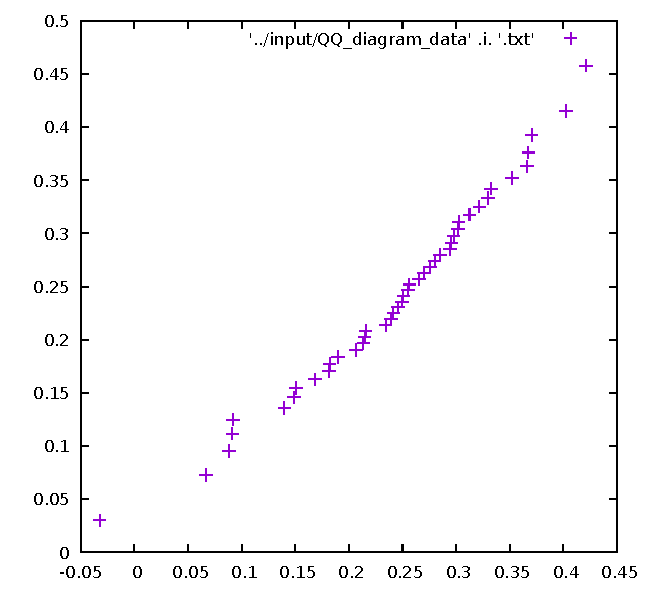
\includegraphics[width=0.3\textwidth]{../PCA/gnuplot/results_qq_diagrams/QQ_diagram4.pdf}}
  \qquad
  \subfloat[Länge der Hand]{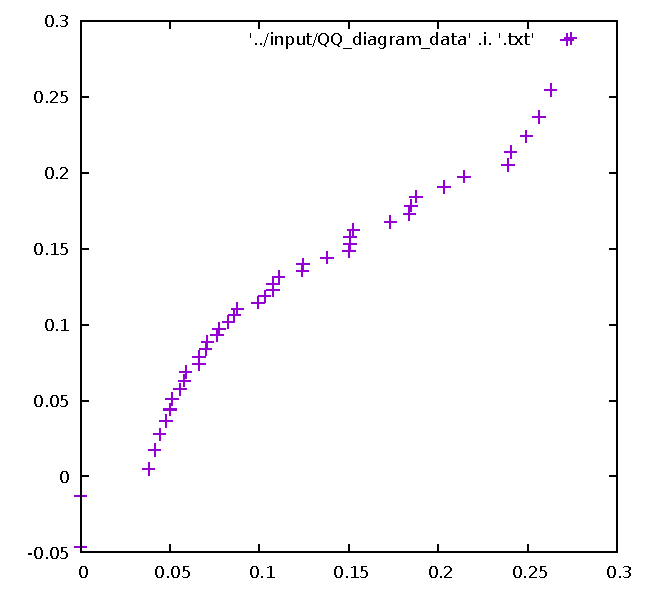
\includegraphics[width=0.3\textwidth]{../PCA/gnuplot/results_qq_diagrams/QQ_diagram24.pdf}}
  \qquad
  \subfloat[Länge des Oberschenkels]{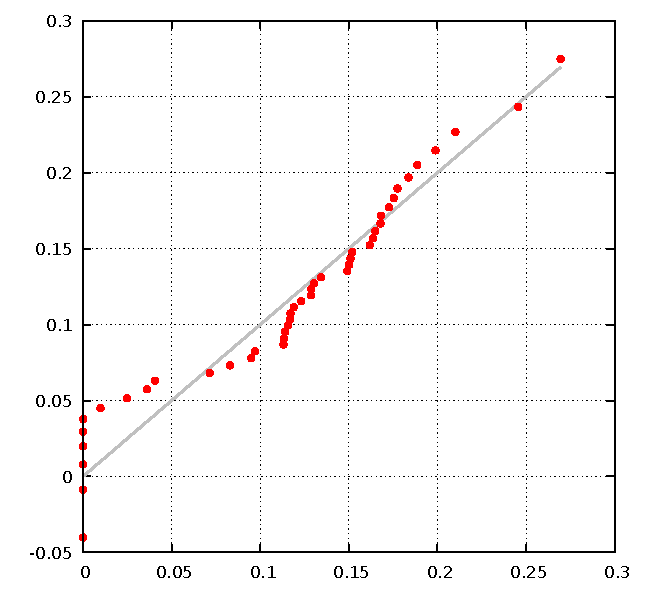
\includegraphics[width=0.3\textwidth]{../PCA/gnuplot/results_qq_diagrams/QQ_diagram25.pdf}}
  
  \caption{Beispielhaft ausgewählte Quantil-Quantil-Diagramme von drei Eingabedimensionen. (a) weicht nicht stark von der Normalverteilung ab, (b) und (c) hingegen schon mehr, sind aber trotzdem noch akzeptabel verteilt.}
  \label{qqdiagram_examples}
 \end{figure}
 
 \begin{figure}
  \subfloat[Gewicht linear]{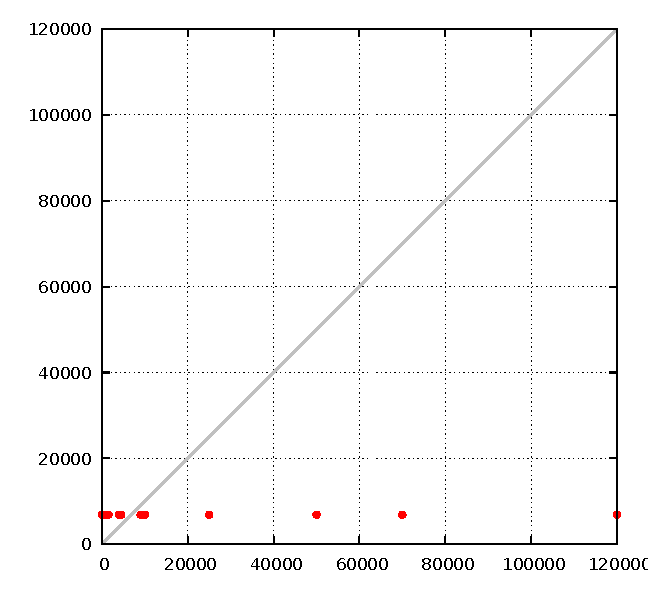
\includegraphics[width=0.3\textwidth]{../PCA/gnuplot/results_qq_diagrams/QQ_diagram_linear_weight.pdf}}
  \qquad
  \subfloat[Gewicht linear (Ausschnitt)]{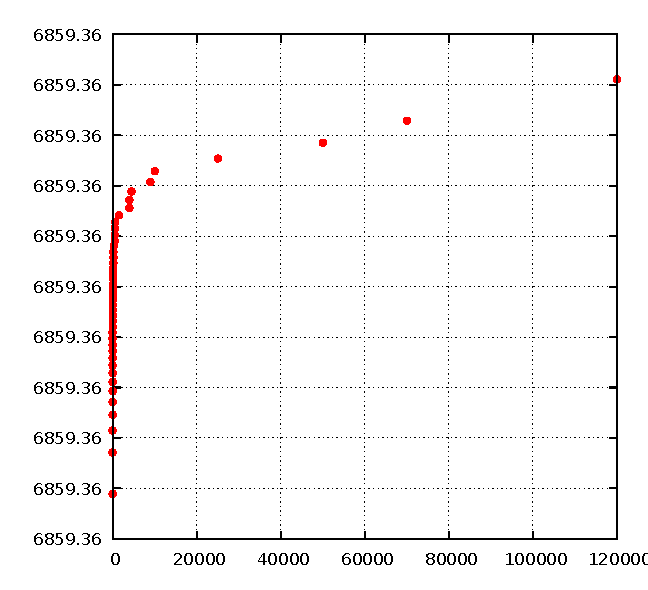
\includegraphics[width=0.3\textwidth]{../PCA/gnuplot/results_qq_diagrams/QQ_diagram_linear_weight_without_diagonal.pdf}}
  \qquad
  \subfloat[Gewicht logarithmisch]{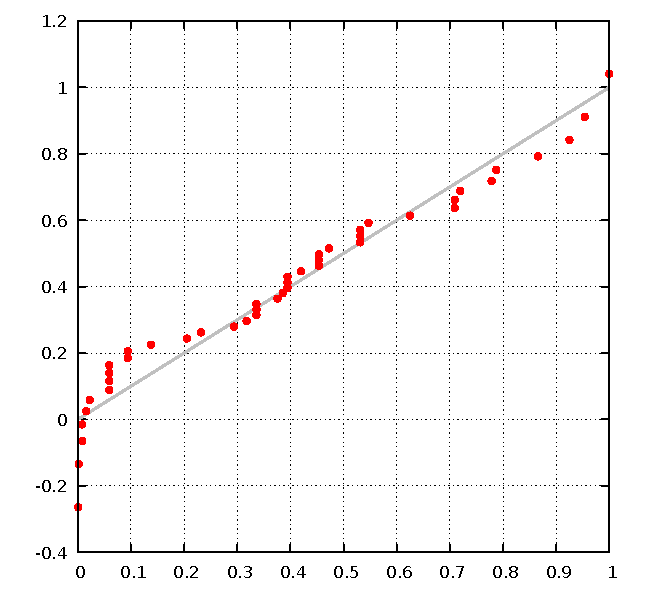
\includegraphics[width=0.3\textwidth]{../PCA/gnuplot/results_qq_diagrams/QQ_diagram28.pdf}}
  
  \caption{ Quantil-Quantil-Diagramme des Gewichts, einmal linear (a,b) und einmal mit logarithmischer Skala (b)}
  \label{qqdiagrams_weight}
 \end{figure}
 
 % Gewichtung der Daten
 Generell bewirkt die Skalierung einer Dimension eine Gewichtung, denn durch eine Skalierung ändert sich die (Ko-)Varianz und somit auch die Kovarianzmatrix. Seien beispielsweise $s,t \in \mathbb{R}$, dann bewirkt eine Skalierung mit $s$ in Dimension $x$ und eine Skalierung mit $t$ in Dimension $y$ eine Skalierung von $s \cdot t$ der Kovarianz Cov$(x,y)$ von $x$ mit $y$, da $\mathrm{Cov}(sx, ty) = (sx - s\mu_x) (ty - t\mu_y) = st \cdot \mathrm{Cov}(x,y)$, mit Erwartungswert $\mu_i$ in \mbox{Dimension $i$}.
 
 Wie genau wurden nun die einzelnen Merkmale nur skaliert?
 
 % Bildkoordinaten + -längen
 Zunächst wurden alle Merkmale auf das Intervall $[0, 1]$ skaliert, damit alle den gleichen Einfluss haben.
 Bei Koordinaten oder Längen im Bild bedeutet das, dass sie durch $1000$ geteilt werden, da sie in Pixeln dargestellt werden und das Bild eine Größe von $1000 \times 1000$ Pixeln hat. Bei Längen wären dabei theoretisch auch Werte größer $1000$px möglich. Solche Längen wären aber unrealistisch und werden deshalb ignoriert.\\
 Koordinaten und Längen im Bild sind diejenigen Merkmale, die hier am interessantesten sind. Deshalb sollten sie den größten Einfluss auf das Ergebnis der PCA haben. Alle anderen Merkmale werden deshalb kleiner skaliert.
 
 % Merkmale nach angenommenem Maximum skalieren?
 Man könnte statt einer Skalierung mit $0.001$ auch für jedes einzelne Merkmal den maximal und minimal angenommenen Wert ermitteln und sie dann so skalieren, dass sie Intervalle gleicher Länge abdecken. Das würde ausgleichen, dass \zb kleine Längen eine kleinere Varianz und damit auch einen kleineren Einfluss haben.
 Es wurde aber die oben beschriebene Variante verwendet, da es natürlich wirkt, dass kleine Merkmale im Bild auch weniger wichtig sind. Falls es in Zukunft Gründe für eine andere Gewichtung gäbe, ließe sich das aber leicht anpassen.
 
 % kleinskalieren von Flügeln, Beinen und Gewicht
 Die diskreten Merkmale \emph{Flügel} und \emph{Beine mit Bodenkontakt} und das logarithmische \emph{Gewicht} wurden zunächst ebenfalls auf das Intervall $[0, 1]$ skaliert. Das bedeutet für das angepasste Gewicht $\bar{w} = \frac{\mathrm{log}(w+1)}{\mathrm{log}(\mathrm{max}+1)}$. Das schwerste Wirbeltier ist der Blauwal mit 120 Tonnen (siehe Abschnitt \ref{bigAndSmall}). Deshalb ist hier max $= 120.000$kg.\\
 Danach wurden die Werte noch einmal durch $100$ geteilt, um ihren Einfluss zu verringern. Das Ziel war, dass diese Merkmale nicht als große Einträge in den größten Eigenvektoren (den "`principal components"') auftauchen. Ohne diese Skalierung sind diese Merkmale recht dominant. Mit der Skalierung hingegen sind sie in den größten Eigenvektoren unter den kleinsten Werten zu finden.
 
 % Projektion auf Eigenvektoren
 Interessant ist die Projektion der Eingabedaten auf die größten beiden  Eigenvektoren. In Abbildung \ref{projections_scales} ist gut zu vergleichen was die Effekte der Skalierung der Eingabedaten sind. Ganz links sind die Ergebnisse zusehen, die entstehen, wenn alle Merkmale nur auf das Intervall $[0, 1]$ skaliert werden. In der Mitte geht das Gewicht nicht mehr linear, sondern logarithmisch ein und ganz rechts sind \emph{Flügel}, \emph{Anzahl Beine} und \emph{Gewicht} zusätzlich klein skaliert. Gut zu sehen ist, wie sich die Clusterbildung durch die Anpassungen verringert.
 
 % Projektion unterschiedlich gelabelt
 In Abbildung \ref{projections_tags} ist noch einmal jeweils die Projektion der skalierten Daten auf die ersten beiden Eigenvektoren zu sehen. Diesmal sind die Daten anhand der verschiedenen diskret erhobenen Merkmale markiert. Es ist \zb schön zu sehen, dass alle Tiere mit Flügeln auch Vögel sind und dass fast alle Tiere, die zwei Beine haben, Vögel sind. Vier Tiere haben zwei Beine, sind aber keine Vögel: die Ohrenrobbe, der Seehund, der Tyrannosaurus Rex und das Känguru.

 \begin{figure}
  \subfloat[gleiche Skalierung aller Dimensionen]{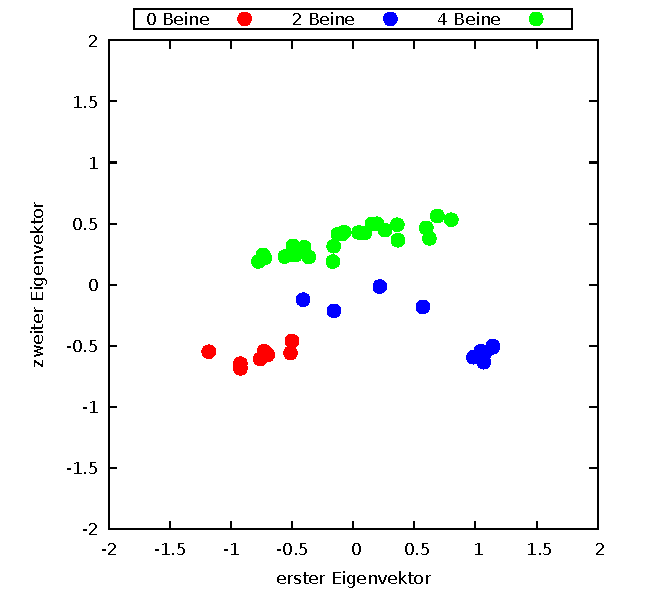
\includegraphics[width=0.3\textwidth]{../PCA/gnuplot/results_with_leg_tag/projection_eigenvectors12.pdf}}
  \qquad
  \subfloat[logarithmisches Gewicht]{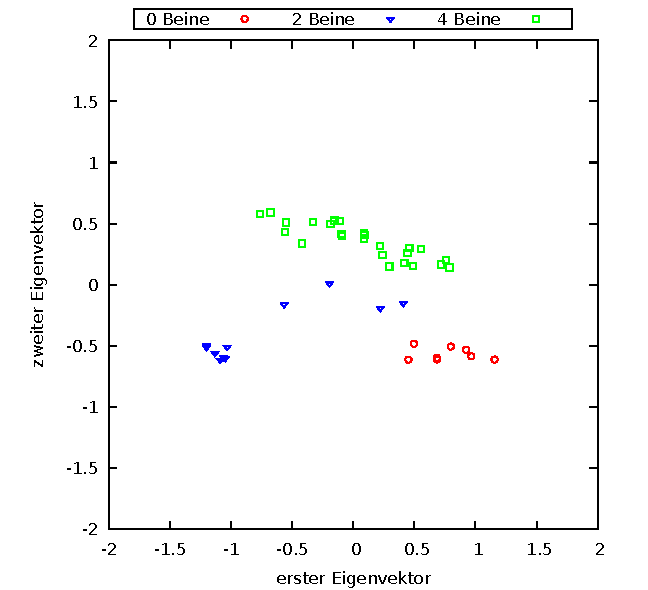
\includegraphics[width=0.3\textwidth]{../PCA/gnuplot_log_weight/results_with_leg_tag/projection_eigenvectors12.pdf}}
  \qquad
  \subfloat[skalierte "`Zusatzmerkmale"']{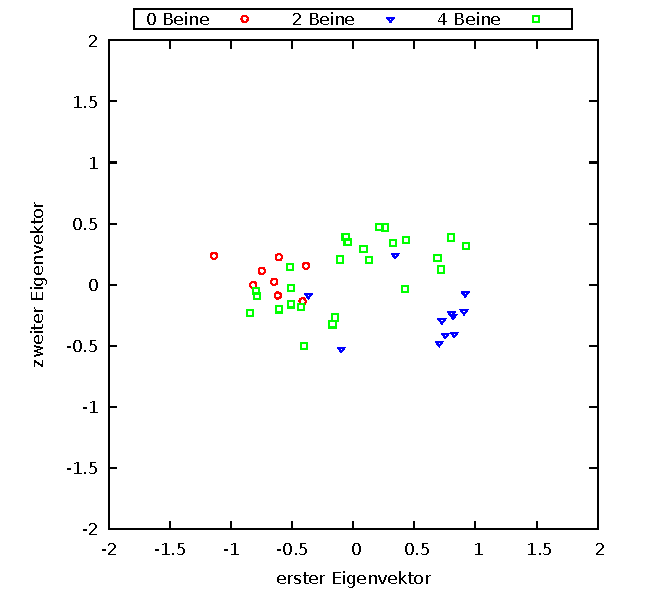
\includegraphics[width=0.3\textwidth]{../PCA/gnuplot_log_weight_with_downscaled_wings_legs_and_weight/results_with_leg_tag/projection_eigenvectors12.pdf}}
  
  \caption{Dargestellt sind hier jeweils die Projektionen der Eingabedaten auf die ersten beiden Eigenvektoren. Für jede Version wurden die Eingabedaten unterschiedlich vorverarbeitet. (a) Skalierung aller erhobenen Daten auf das Intervall $[0, 1]$, (b) zusätzlich Verwendung von logarithmischem Gewicht, statt linearem, (c) zusätzliche Skalierung der Merkmale \emph{Flügel}, \emph{Anzahl Beine} und \emph{Gewicht} mit $0,01$. In \mbox{Version (b)} wurde der erste Eigenvektor durch die PCA umgedreht, weshalb das Cluster der Zweibeiner auf der linken, statt der rechten Seite zu sehen ist.}
  \label{projections_scales}
 \end{figure}
 
 \begin{figure}
  \subfloat[Flügel]{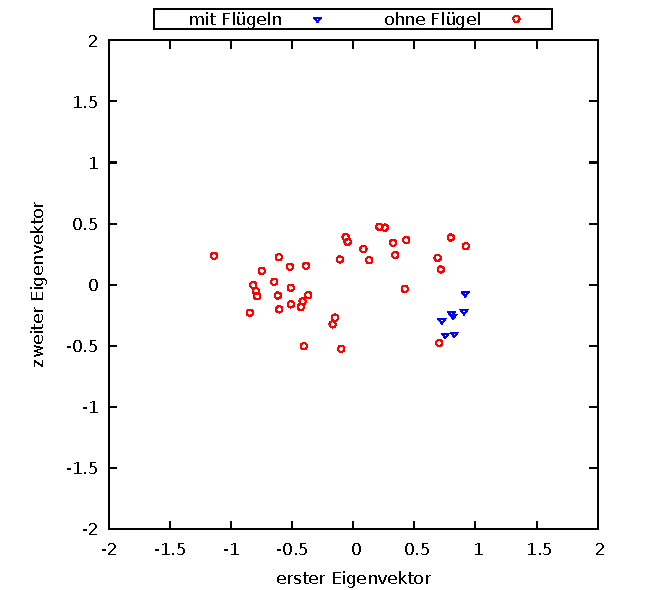
\includegraphics[width=0.3\textwidth]{../PCA/gnuplot_log_weight_with_downscaled_wings_legs_and_weight/results_with_wing_tag/projection_eigenvectors12.pdf}}
  \qquad
  \subfloat[Anzahl Beine mit Bodenkontakt]{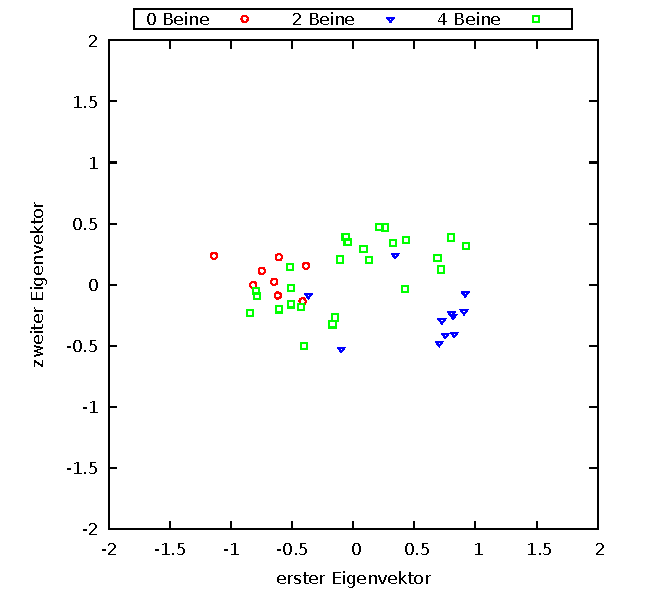
\includegraphics[width=0.3\textwidth]{../PCA/gnuplot_log_weight_with_downscaled_wings_legs_and_weight/results_with_leg_tag/projection_eigenvectors12.pdf}}
  \qquad
  \subfloat[Tierklasse]{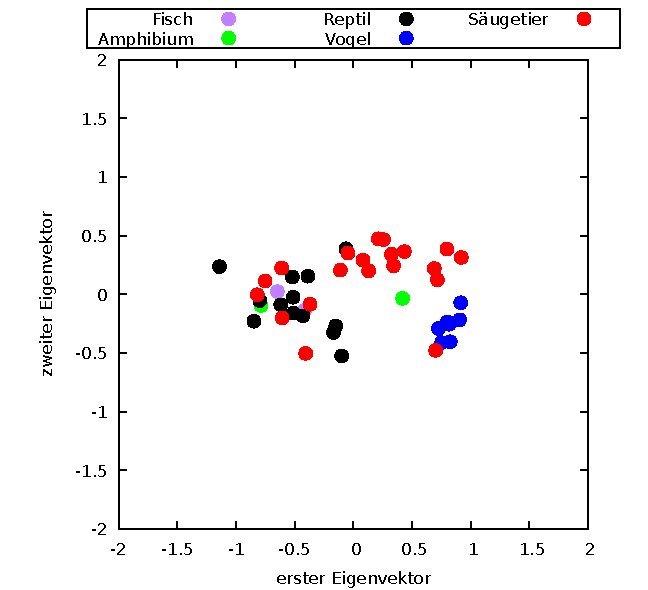
\includegraphics[width=0.3\textwidth]{../PCA/gnuplot_log_weight_with_downscaled_wings_legs_and_weight/results_with_animal_class_tag/projection_eigenvectors12.pdf}}
  
  \caption{Projektion der, wie in Abbildung \ref{projections_scales}c skalierten, Eingabedaten auf die Ebene, die durch den ersten und zweiten Eigenvektor aufgespannt wird. Markiert sind jeweils ob Flügel vorhanden sind (a), die Anzahl der Beine (b) und die \mbox{Tierklasse (c)}.}
  \label{projections_tags}
 \end{figure}
 
 
 % Ergebnis wieder normalverteilt
 Auch im Koordinatensystem der Eigenvektoren sollten die Daten wieder normalverteilt sein. Dies wurde ebenfalls mit Quantil-Quantil-Diagrammen untersucht. In Abbildung \ref{qqdiagram_projections} sind die Ergebnisse für die ersten drei Eigenvektoren zu sehen. Es gibt, wie bei den Eingabedaten, keine allzu großen Abweichungen.
 
 \begin{figure}
  \subfloat[erster Eigenvektor]{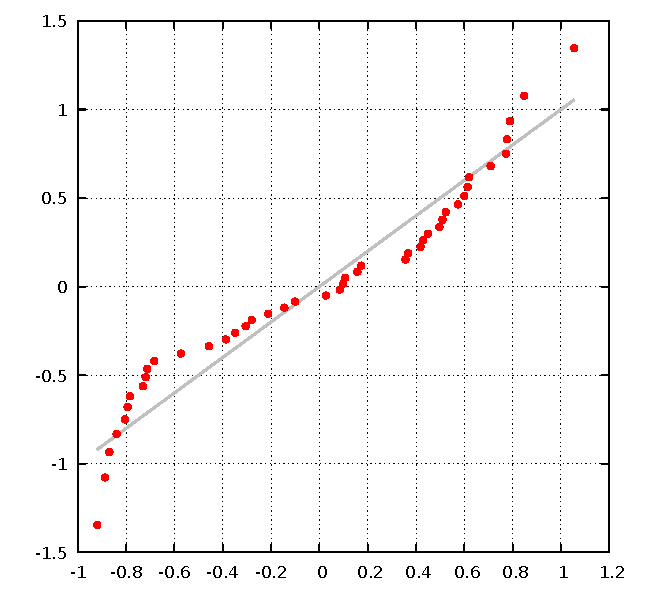
\includegraphics[width=0.3\textwidth]{../PCA/gnuplot_log_weight_with_downscaled_wings_legs_and_weight/results_qqdiagrams/QQ_diagram_projection0.pdf}}
  \qquad
  \subfloat[zweiter Eigenvektor]{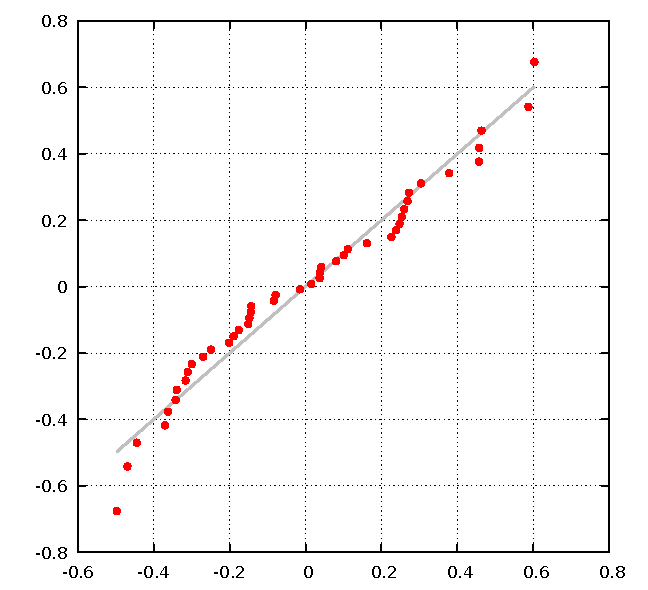
\includegraphics[width=0.3\textwidth]{../PCA/gnuplot_log_weight_with_downscaled_wings_legs_and_weight/results_qqdiagrams/QQ_diagram_projection1.pdf}}
  \qquad
  \subfloat[dritter Eigenvektor]{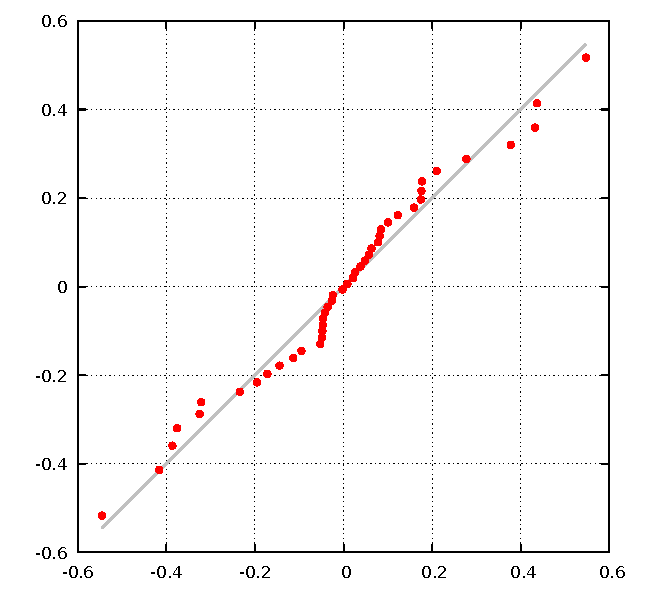
\includegraphics[width=0.3\textwidth]{../PCA/gnuplot_log_weight_with_downscaled_wings_legs_and_weight/results_qqdiagrams/QQ_diagram_projection2.pdf}}
  
  \caption{Quantil-Quantil-Diagramme der Eingabedaten projiziert auf die größten drei Eigenvektoren.}
  \label{qqdiagram_projections}
 \end{figure}
 
 
 % Mittelwert
 Der Mittelwert der skalierten Eingabedaten ist in Abbildung \ref{mean} visualisiert.
 Wie auch bei der Datenerhebung ist hier die Position der Wirbelsäule in einem $1000 \times 1000$ Pixel Bild gezeigt. Da von den Knochen der Vorder- und Hinterextremitäten nur die Längen erhoben wurden, sind ihre Positionen nicht realistisch. Die restlichen Daten sind nicht visualisiert, sondern nur in Textform angegeben.
 
 \begin{figure}
  \centering
  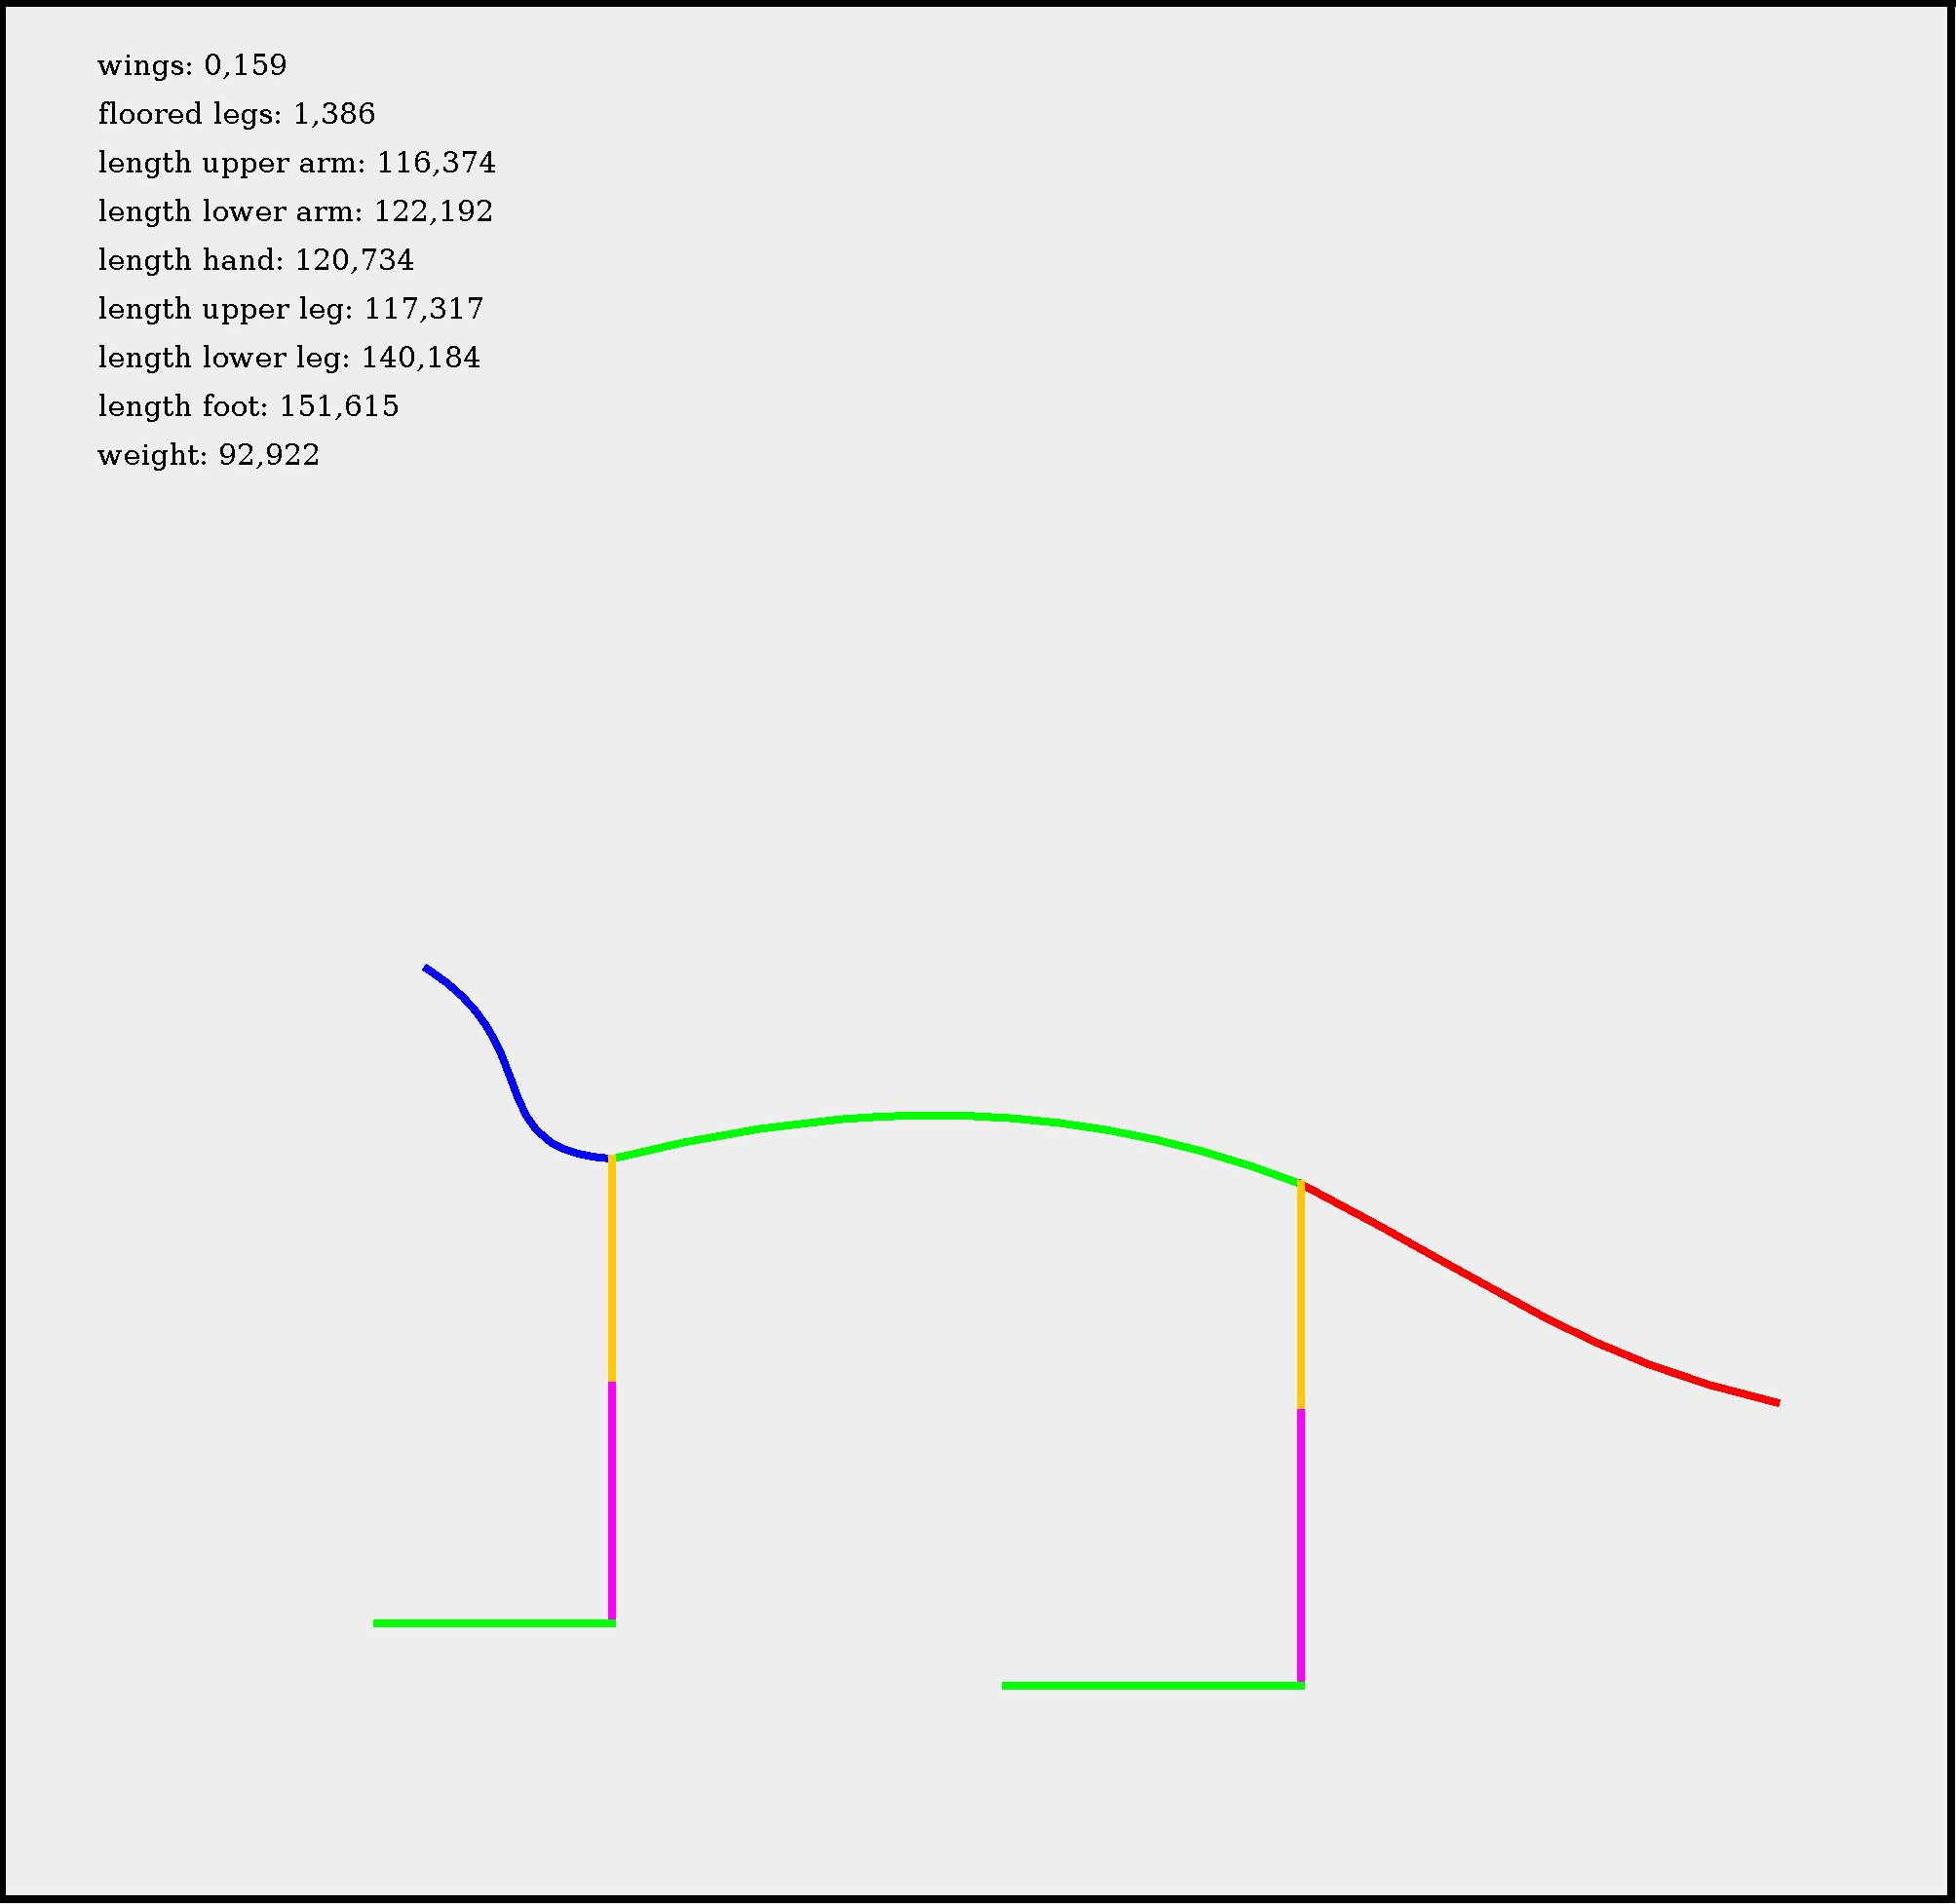
\includegraphics[width=0.5\textwidth]{../PCA/mean_log_weight_downscaled_wings_legs_and_weight(onlyBox,stroke4).jpg}
  \caption{Visualisierung des Mittelwerts der skalierten Eingabedaten. Die Werte, die nicht grafisch visualisiert sind, sind folgende: \emph{Flügel} $0,159$, \emph{Beine mit Bodenkontakt} $1,39$, \emph{Gewicht} $93$kg.}
  \label{mean}
 \end{figure}
 
 % min Abstand
 Den minimalen Abstand zum Mittelwert hat der Klippschliefer (siehe Abbildung \ref{klippschliefer_farbig}). Zusätzlich zum Bild wurde für den Klippschliefer folgende Daten erhoben:
 \emph{Tierklasse} Säugetier, \emph{Flügel} nein, \emph{Anzahl Beine mit Bodenkontakt} $4$, \emph{Gewicht} $4$kg.
 
 % max Abstand
 Den maximalen Abstand hat die Schlange. Die erhobenen Daten sind hier:
 \emph{Tierklasse} Reptil, \emph{Flügel} nein, \emph{Anzahl Beine mit Bodenkontakt} $0$, \emph{Gewicht} $50$kg.\\
 Die Schlange ist allerdings das einzige Tier zu dem es kein "`echtes"' Bild des Skeletts gibt. Das liegt daran, dass es keine seitlichen Abbildungen von ausgestreckten Schlangen gibt. Sie werden eigentlich immer gekrümmt dargestellt, da sonst das Bild sehr lang und schmal werden würde. Deshalb wurde für die Schlange nur eine horizontale Linie knapp über dem unteren Bildrand eingezeichnet, die den Rücken darstellen soll. Extremitäten und ersichtliche Punkte an denen der Rücken in Hals oder Schwanz übergeht gibt es bei Schlangen nicht.
 
 % zweitgrößter Abstand (da max Schlange)
 Der Punkt mit dem zweitgrößten Abstand zum Mittelwert ist das Känguru (siehe Abbildung \ref{kaenguru_farbig}). Zusätzlich zum Bild gibt es hier folgende Daten:
  \emph{Tierklasse} Säugetier, \emph{Flügel} nein, \emph{Anzahl Beine mit Bodenkontakt} $2$, \emph{Gewicht} $50$kg
  
 \begin{figure}
  \subfloat[Klippschliefer]{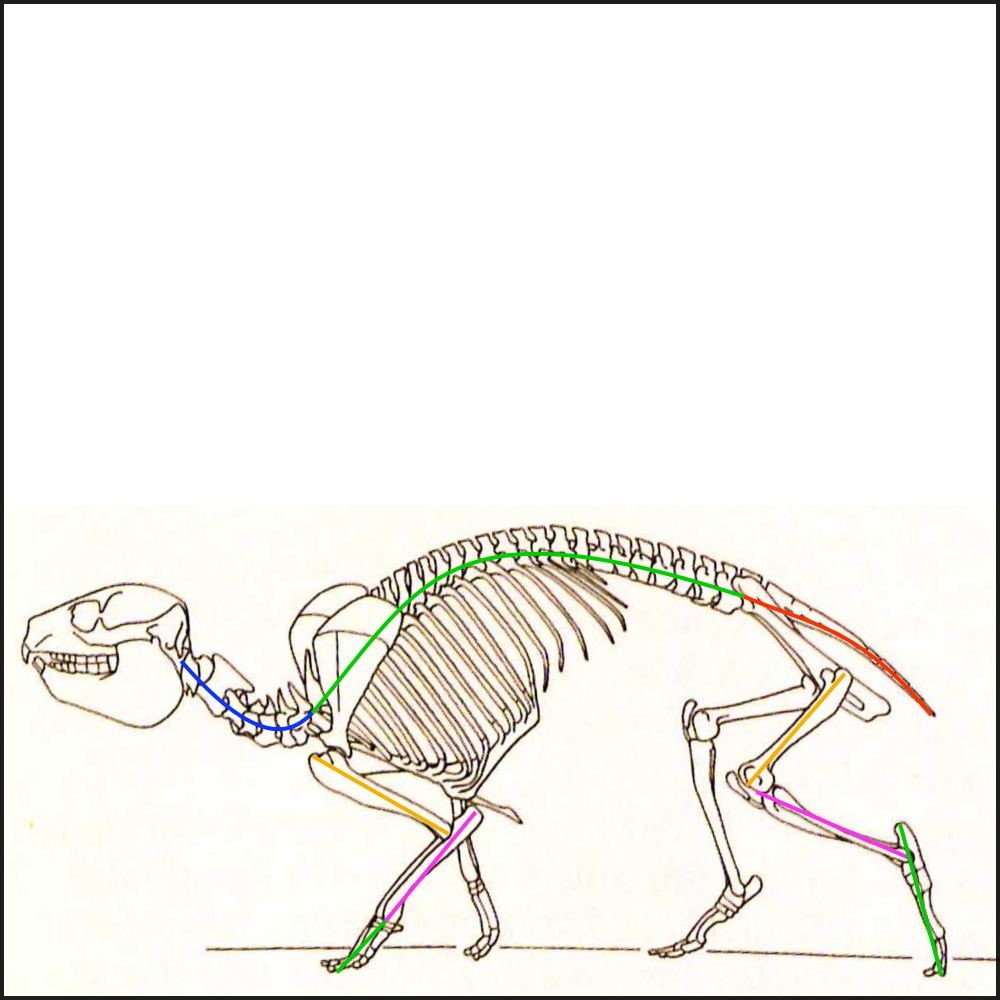
\includegraphics[width=0.5\textwidth]{../PCA/Skelettbilder/Klippschliefer_farbig.png} \label{klippschliefer_farbig}}
  \qquad
  \subfloat[Känguru]{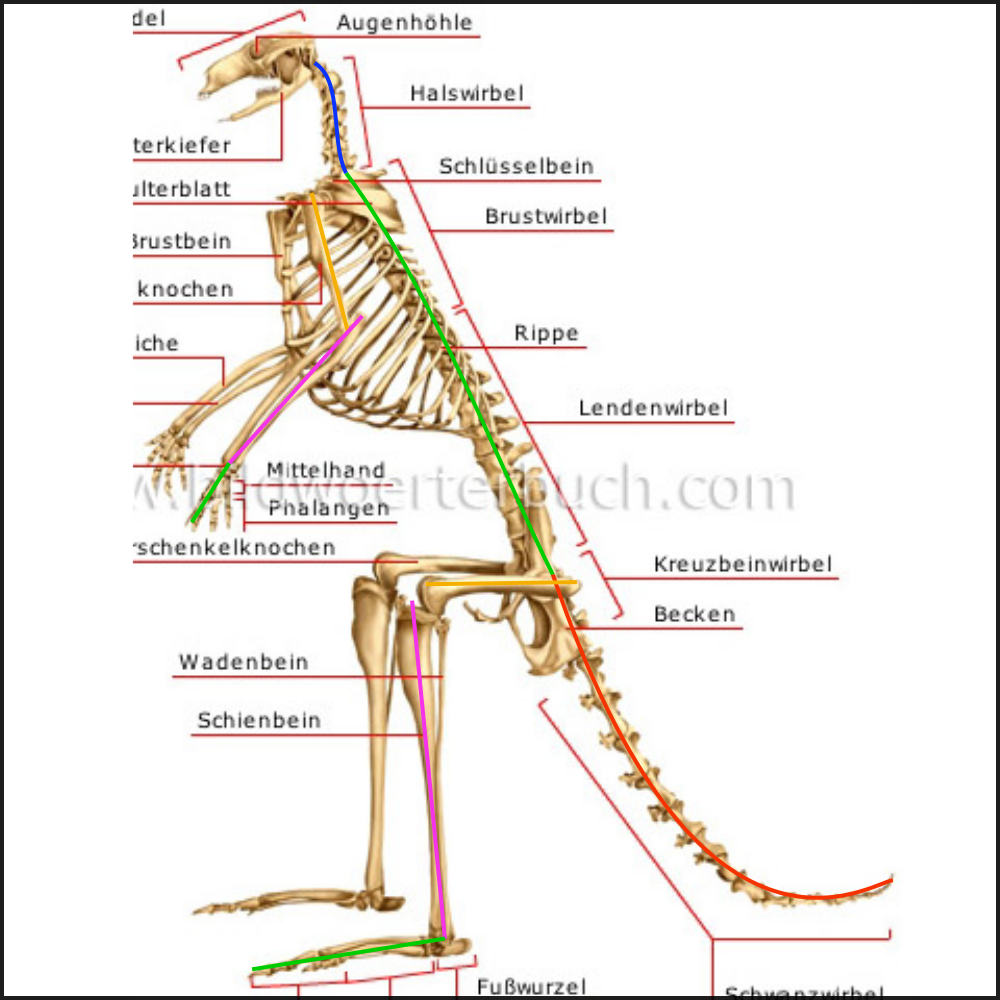
\includegraphics[width=0.5\textwidth]{../PCA/Skelettbilder/Kaenguru_farbig.png}\label{kaenguru_farbig}}
  
  \caption{Annotierte Bild des Skeletts eines Klippschliefers (a) und eines \mbox{Kängurus (b)}. Die Teile der Wirbelsäule und die Knochen der Extremitäten sind hier jeweils mit der gleichen Farbe markiert wie in der Visualisierung des Mittelwerts (Abbildung \ref{mean})}
 \end{figure}
 

 %-----------------------------------
 \section{Analyse der Ergebnisse}
 \label{section_pca_result_analysis}
 
 % Eigenvektoren und Rekonstruktionen
 Zu $29$ Eingabedimensionen gibt es auch $29$ Eigenvektoren mit Eigenwerten größer $0$. Der kleinste hat einen Eigenwert von $0,000001$. Von den Eigenwerten sind $6$ größer als $0,01$. Leider reichen diese $6$ Dimensionen noch nicht aus, um die Eingabedaten hinreichend anzunähern. Bei manchen Tieren funktioniert das zwar ganz gut (siehe Archaeopteryx, Abbildung \ref{archaeopteryx}), bei anderen aber eher schlechter (siehe Frosch, Abbildung \ref{frosch}).
 Die Daten konnten somit von der PCA nicht sehr gut komprimiert werden. Trotzdem sind die berechneten Eigenvektoren hilfreich um zufällige Punkte mit der Verteilung der Eingabebeispiele zu generieren (wie auch beschrieben in Abschnitt \ref{PCA}).
 
 \begin{figure}
  \subfloat[Rekonstruktion aus 6 Eigenvektoren]{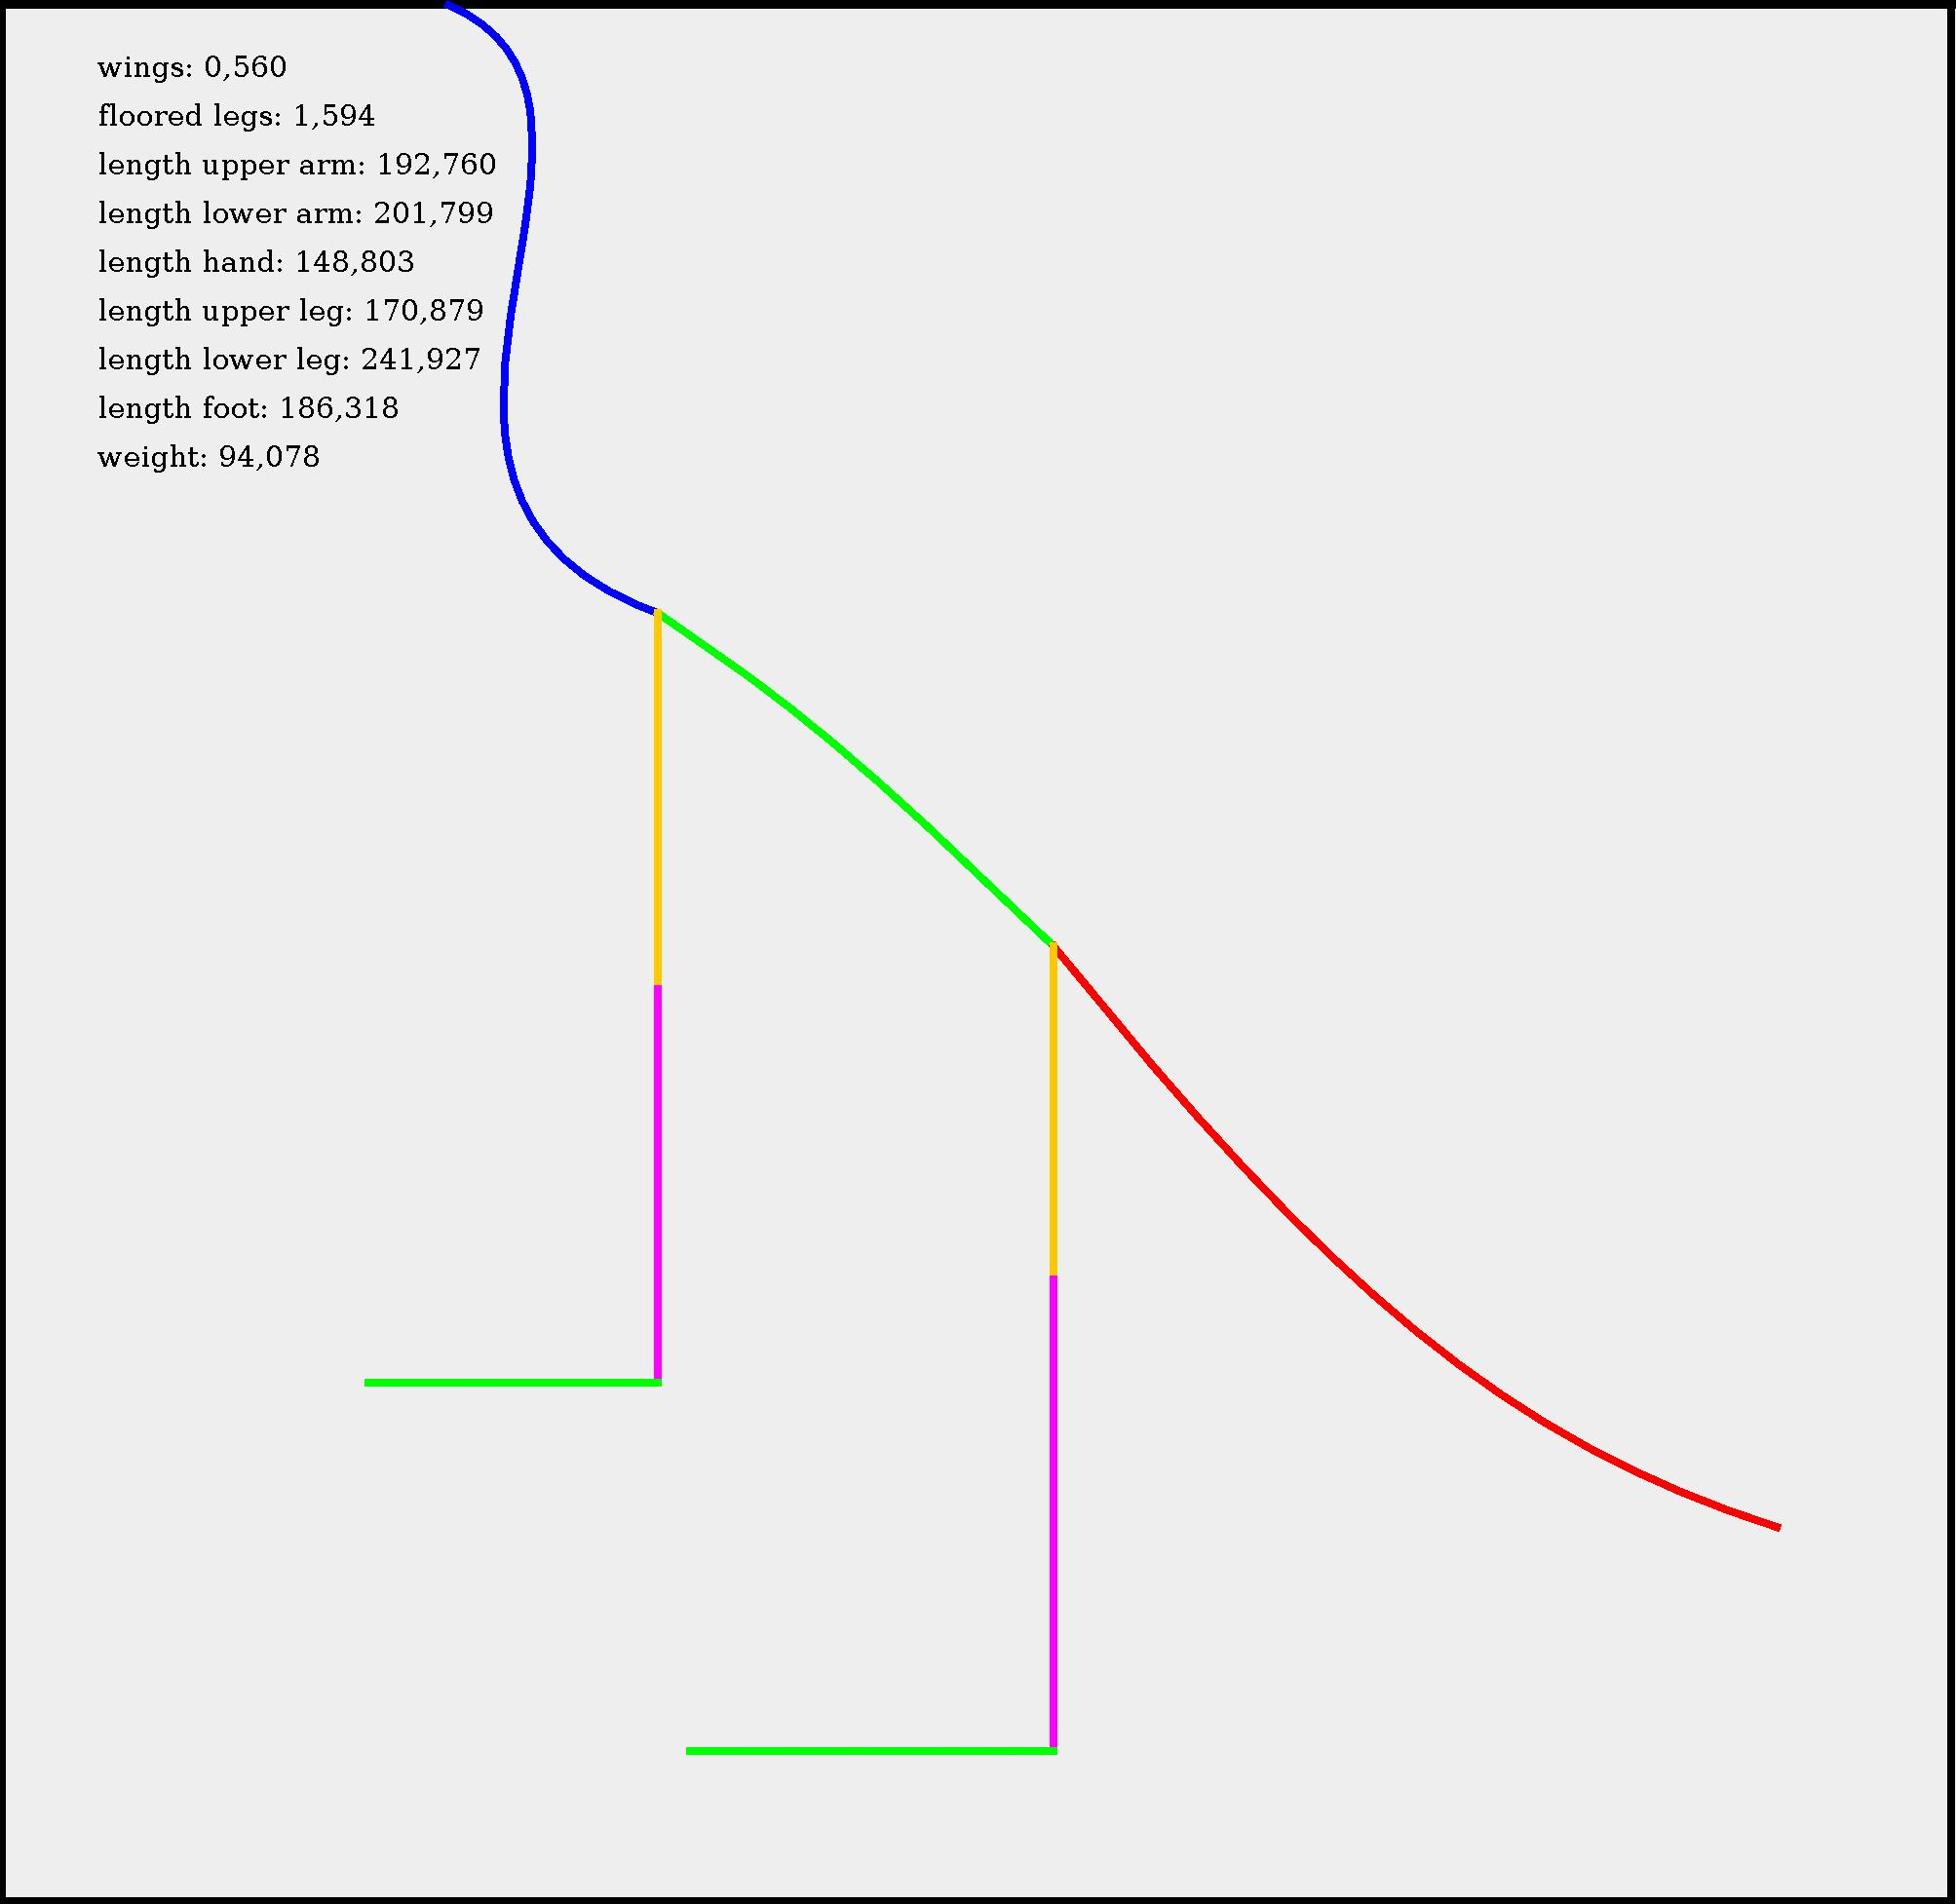
\includegraphics[width=0.5\textwidth]{../PCA/animal_reconstructions_log_weight_downscaled_wings_legs_and_weight/6EV/Archaeopteryx_Ausschnitt.jpg}}
  \qquad
  \subfloat[Eingabebild]{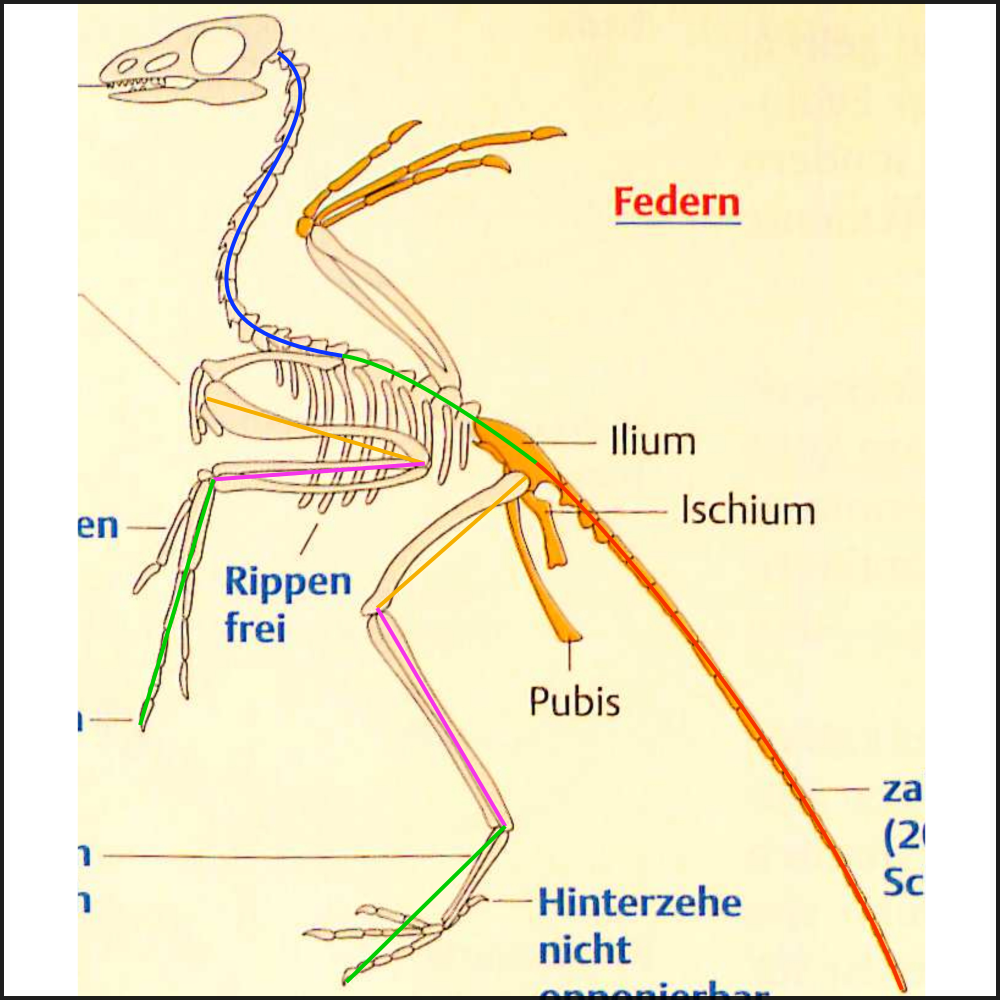
\includegraphics[width=0.5\textwidth]{../PCA/Skelettbilder/Archaeopteryx_farbig.png}}
  
  \caption{Archaeopteryx (a) Rekonstruktion aus den größten $6$ Eigenvektoren, nicht visualisierte Daten: \emph{Flügel} $0,56$, \emph{Beine mit Bodenkontakt} $1,594$, \emph{Gewicht} $94,1$kg\\ 
  (b) Eingabebild}
  \label{archaeopteryx}
 \end{figure}
 
\begin{figure}
  \subfloat[$6$ Eigenvektoren,
  \emph{Flügel} $0,4$, \emph{Beine mit Bodenkontakt} $1,27$, \emph{Gewicht} $90,2$kg]
  {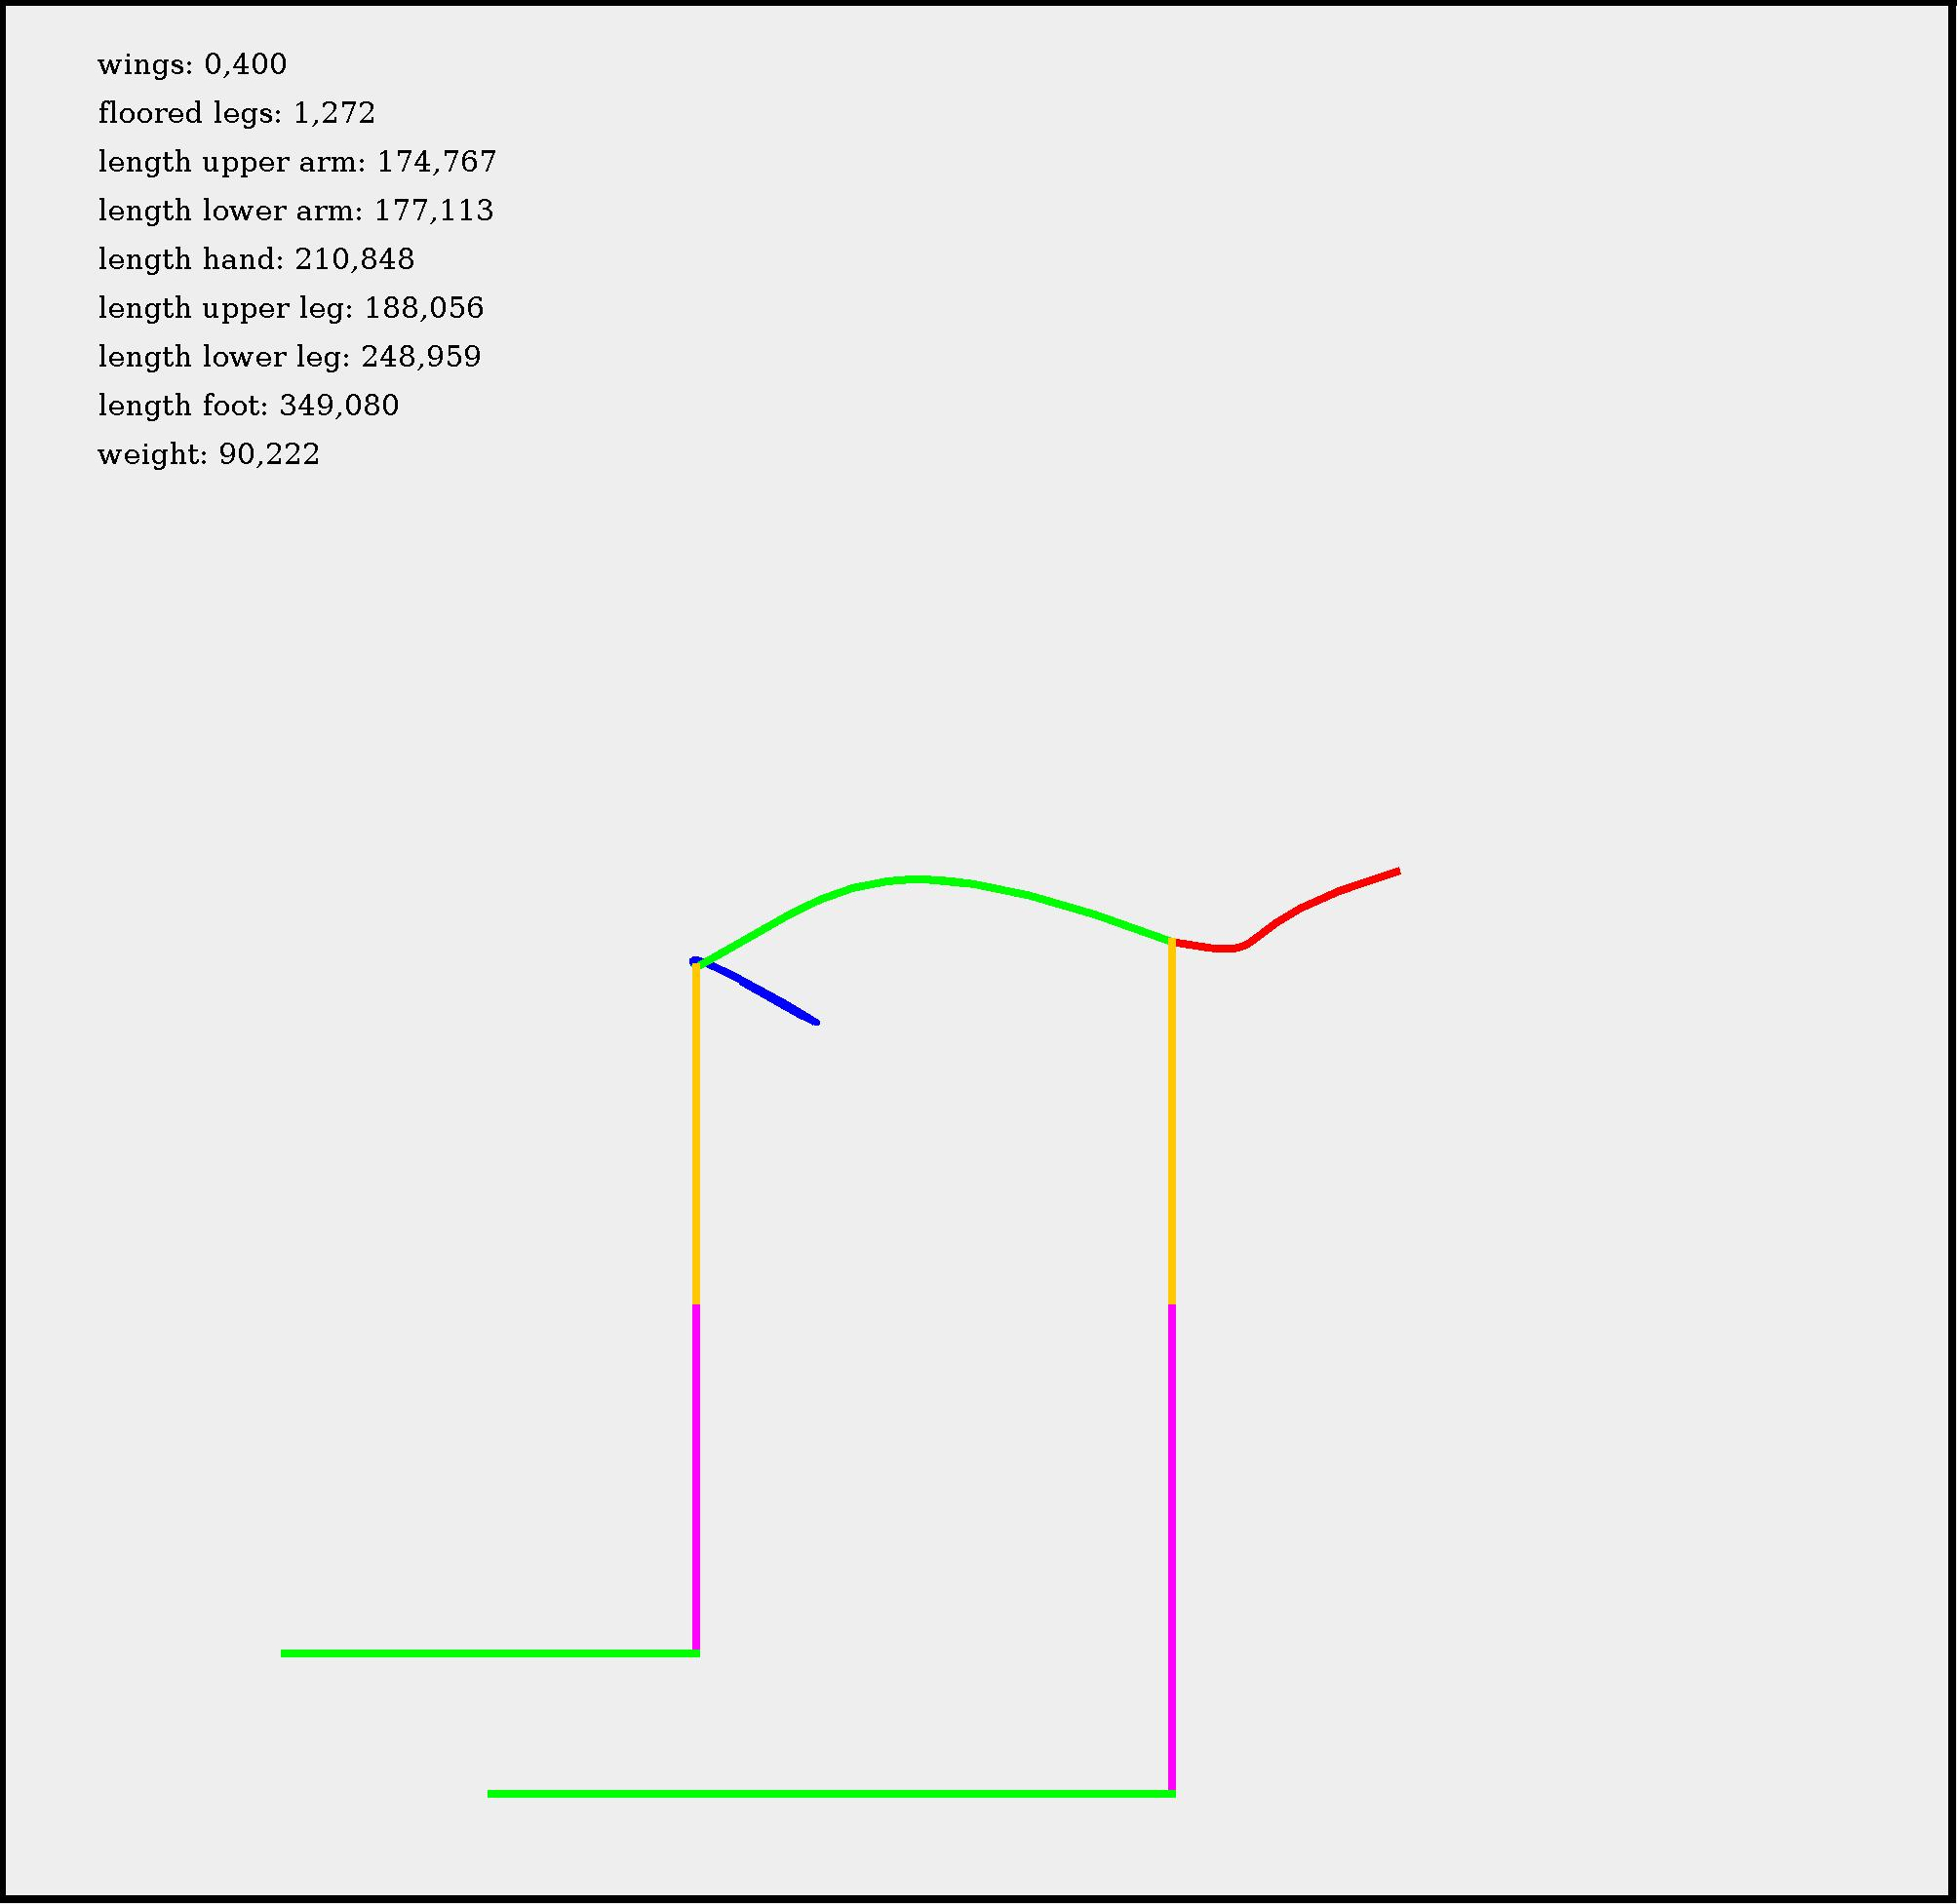
\includegraphics[width=0.5\textwidth]{../PCA/animal_reconstructions_log_weight_downscaled_wings_legs_and_weight/6EV/Frosch_Ausschnitt.jpg}}
  \qquad
  \subfloat[$10$ Eigenvektoren,
  \emph{Flügel} $0,151$, \emph{Beine mit Bodenkontakt} $1,28$, \emph{Gewicht} $88,7$kg]{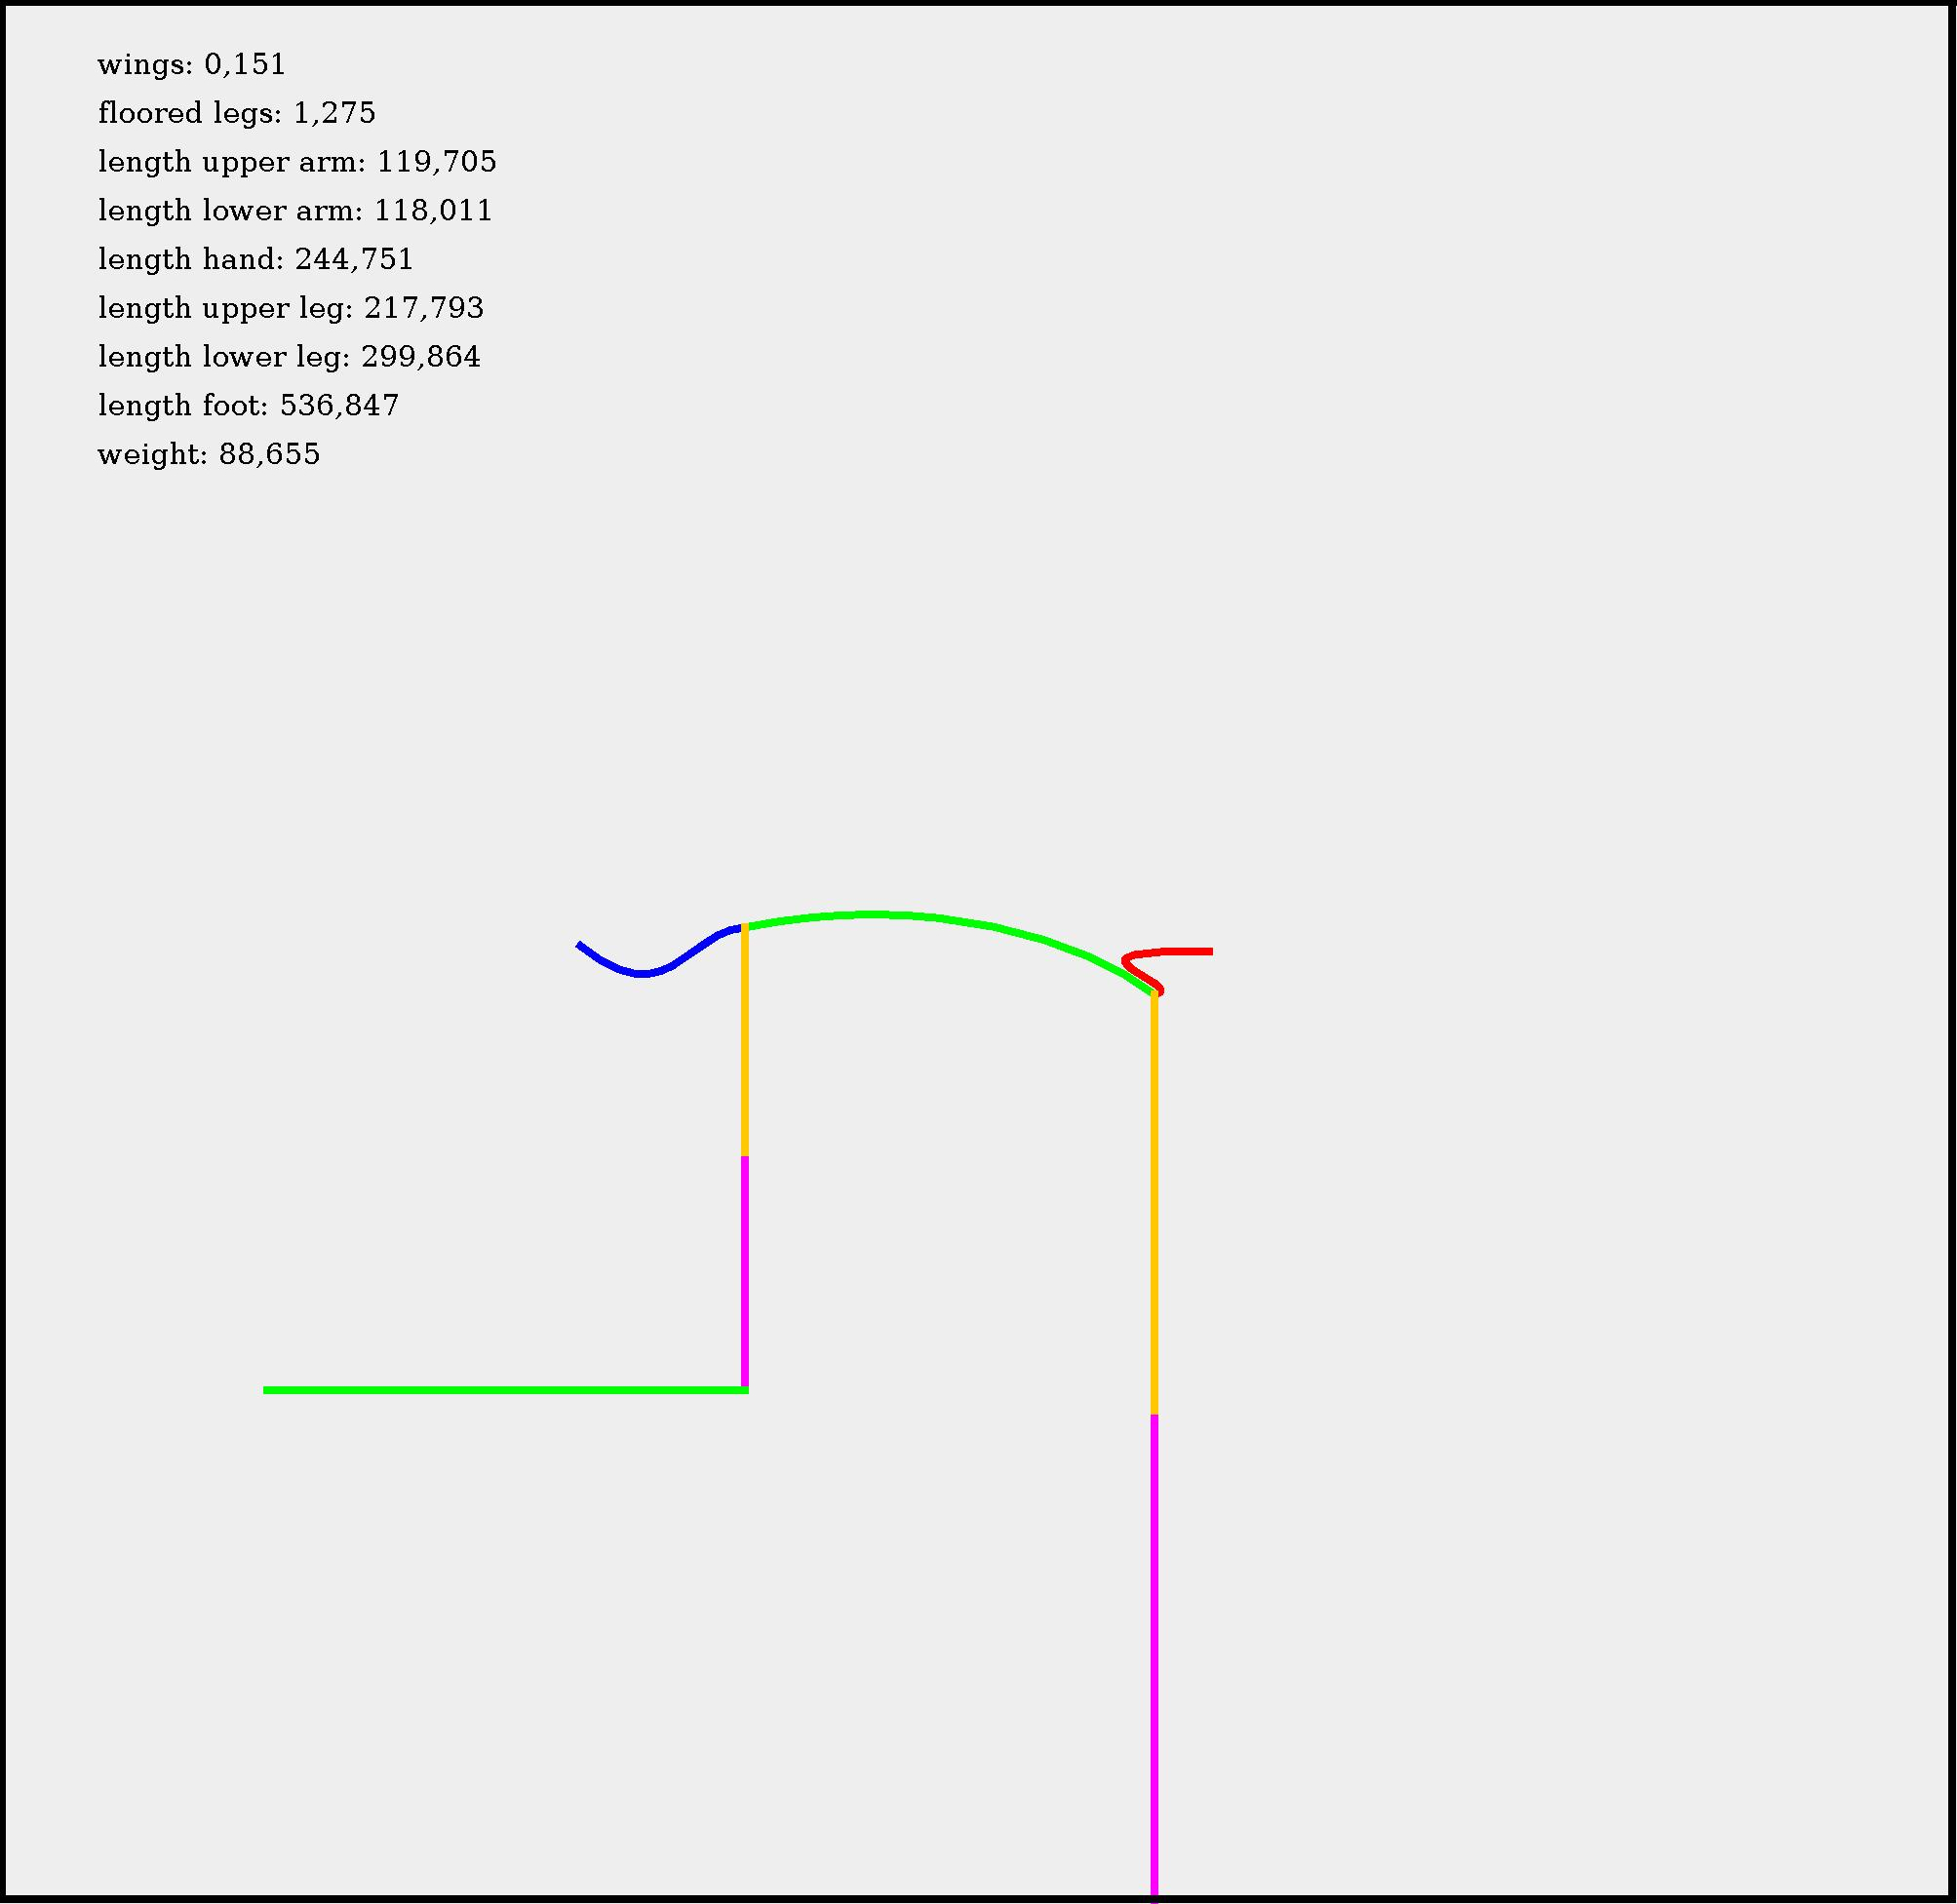
\includegraphics[width=0.5\textwidth]{../PCA/animal_reconstructions_log_weight_downscaled_wings_legs_and_weight/10EV/Frosch_Ausschnitt.jpg}}
  \\
  \subfloat[$20$ Eigenvektoren,
  \emph{Flügel} $0,217$, \emph{Beine mit Bodenkontakt} $1,7$, \emph{Gewicht} $89,2$kg]
  {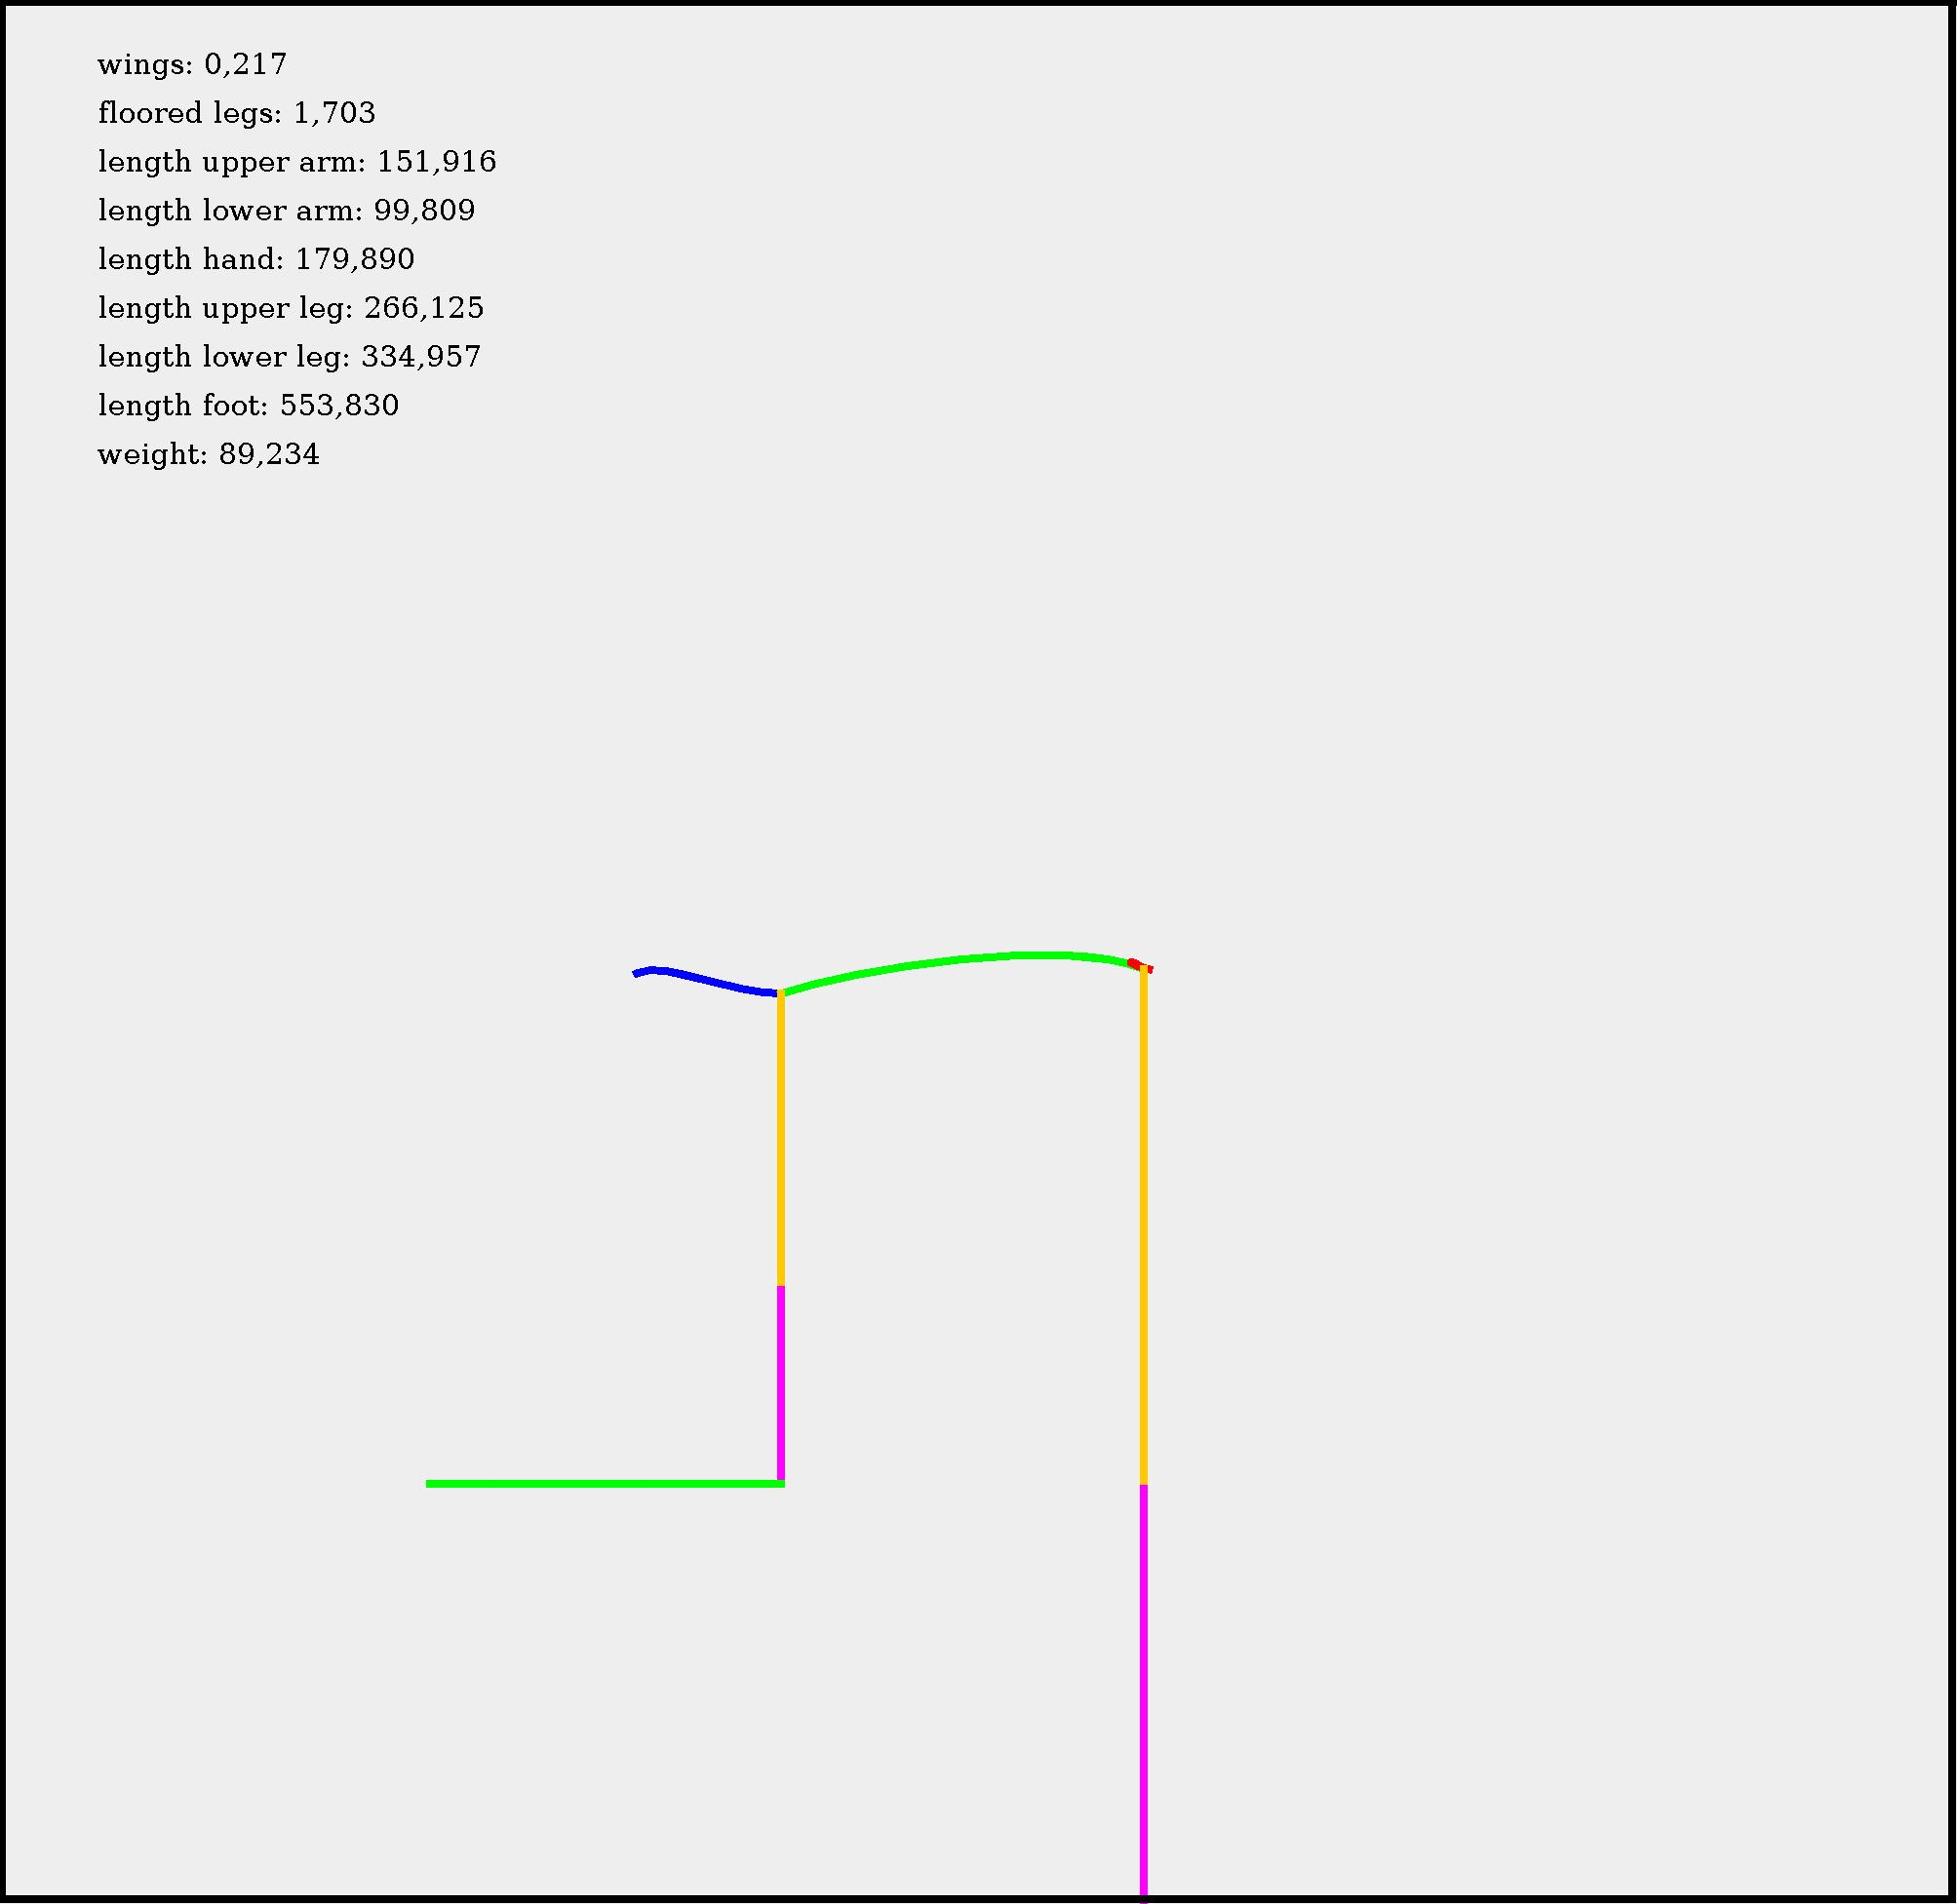
\includegraphics[width=0.5\textwidth]{../PCA/animal_reconstructions_log_weight_downscaled_wings_legs_and_weight/20EV/Frosch_Ausschnitt.jpg}}
  \qquad
  \subfloat[Eingabebild]{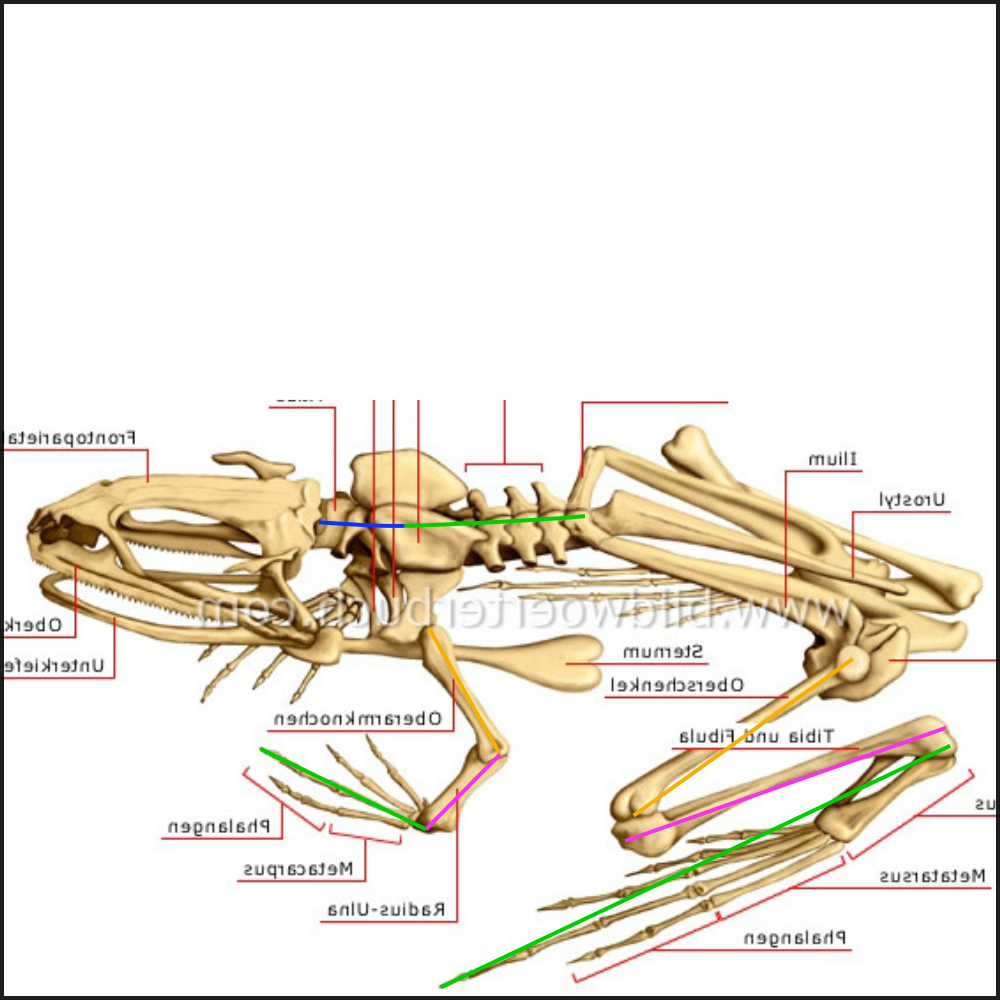
\includegraphics[width=0.5\textwidth]{../PCA/Skelettbilder/Frosch_farbig.png}}
  
  \caption{Frosch, Rekonstruktionen aus den größten $6$, $10$ und $20$ Eigenvektoren und das Eingabebild (d). Nicht visualisierte Dimensionen sind jeweils unter dem entsprechenden Bild angegeben. Zusätzlich zum Eingabebild erhobene Daten sind:
  \emph{Tierklasse} Amphibie, \emph{Flügel} $0$, \emph{Beine mit Bodenkontakt} $2$, \emph{Gewicht} $0,01$kg.}
  \label{frosch}
 \end{figure}

 Bei allen Eingabedimension, außer der Position der Wirbelsäule, kann man die Frage stellen, ob sie nötig sind, oder ob sie die Ergebnisse der PCA eher verschlechtern. Deshalb wurde ausprobiert verschiedene (Kombinationen von) Merkmalen wegzulassen. Die Ergebnisse unterscheiden sich aber nicht extrem von der PCA mit allen Daten. \\
 Leider gibt es keine gute Möglichkeit die Qualität der Ergebnisse der PCA zu messen. Man könnte den Unterschied zwischen den Eingabedaten und den Rekonstruktionen aus den Linearkombinationen der Eigenvektoren mit den größten Eigenwerten messen. Aber das liefert, durch das Fehlen von verschiedenen Dimensionen kein einheitliches Maß.
 Da jede Dimension dem Algorithmus, der später Skelette generieren soll, helfen könnte, wurde kein Merkmal verworfen.
 
 Außerdem gibt es die Möglichkeit die Eingabedaten in mehrere Mengen aufzuteilen und diese einzeln zu analysieren. Hierbei gibt es zunächst das Problem, dass sich dann die Anzahl der Datenpunkte noch weiter reduziert, was die Ergebnisse nicht mehr repräsentativ macht.
 Merkmale, die sich zur Unterteilung in Mengen anbieten würden, sind die diskreten, also \emph{Flügel} und \emph{Beine mit Bodenkontakt}. Sie sind auch klar als Cluster im Koordinatensystem der PCA ohne angepasste Skalierung zu erkennen (Abbildung \ref{projections_scales} a und b).
 Getestet wurde die Aufteilung anhand der Werte für die Flügel, da sich dadurch nur zwei Gruppen ergeben. Tatsächlich liefert sie bessere Rekonstruktionen aus den größten Eigenvektoren. Das liegt aber natürlich in erster Linie daran, dass die zu untersuchende Datenmenge, jeweils verkleinert wurde.
 
 Ein weiteres Problem daran die Daten in mehrere Mengen aufzuteilen ist, dass dann keine Skelette mehr erzeugt werden können, die zwischen den beiden Gruppen liegen. Tatsächlich scheinen aber die Datenpunkte, die "`zwischen"' den Gruppen erzeugt werden, relativ sinnvoll auszusehen.
 Auch das ist ein Argument dafür keine Aufteilung vorzunehmen.
 
 \todo{Beispiele für zufällig erzeugte Punkte}
 
 
 %-------------------------------------------------
 \section{Bedingte Verteilungen}
 \label{pca_conditions}
 
 
 Aus den Ergebnissen der PCA lassen sich sehr gut zufällige Skelette erzeugen. Es ist aber schwer gezielt Eigenschaften festzulegen.
 Der erste Schritt dies zu erreichen ist Eigenschaften, die so schon in den erhobenen Daten vorkommen, auf gewählte Werte festzulegen. Das können beispielsweise die Anzahl der Beine sein oder ob das Skelett Flügel haben soll.
 
 Dazu kann man, statt die ursprünglichen Daten und deren Verteilung zu verwenden, die entsprechenden bedingten Verteilungen bilden. Dazu muss der bedingte Mittelwert und die bedingte Kovarianzmatrix, wie in \cite{conditionalDistribution} (S.\ $116$ f.) beschrieben, bestimmt werden.
 
 Seien 
 \[x = \begin{pmatrix} x_1 \\ x_2 \end{pmatrix}, 
  \mu = \begin{pmatrix} \mu_1 \\ \mu_2 \end{pmatrix} \text{und } 
  \Sigma = \begin{pmatrix} \Sigma_{11} & \Sigma_{12} \\ \Sigma_{21} & \Sigma_{22} \end{pmatrix} \] 
 
 Der Zufallsvektor $x$ enthält $n$ normalverteilte Zufallsvariablen, $q$ Variablen im Vektor $x_1$ und $n - q$ in $x_2$. Die Einträge in $\mu$ sind die jeweils zugehörigen Mittelwerte und $\Sigma$ ist die Kovarianzmatrix. Die Verteilung für $x_1$ unter der Bedingung, dass $x_2 = b$ hat den Mittelwert $\bar{\mu}$ und Kovarianzmatrix $\overline{\Sigma}$ mit
 
 \[ \bar{\mu} = \mu_1 + \Sigma_{12} \Sigma_{22}^{-1} (b - \mu_2), 
    \overline{\Sigma} = \Sigma_{11} - \Sigma_{12} \Sigma_{12}^{-1} \Sigma_{21} \]
 
 Verwendet man nun $\overline{\Sigma}$ als Eingabe für die PCA, so erhält man nur noch Daten für Skelette unter den vorher festgelegten Bedingungen $b$. Zu beachten ist hier, dass die Eigenvektoren sich im Vergleich zur PCA ohne Bedingungen verändern. Falls man diese also zur Bestimmung eines Datenpunktes verwendet hat (\zb in einer Benutzeroberfläche), so müssen die Werte für die neuen Eigenvektoren neu ausgerechnet werden.
 
 % feste Werte variieren
 Erzeugt man nun in diesem bedingten Raum zufällige Beispiele, zeigt sich sehr deutlich, dass das Festlegen von nur einer Dimension auch die anderen Dimensionen stark einschränken kann. Legt man \zb die Anzahl der Beine fest, so haben die Skelette, die dann bedingt zufällig generiert werden, eine recht geringe Varianz. Das ist daran zu erkennen, dass der Verlauf der Wirbelsäule sehr ähnlich ist (siehe Abbildung \ref{spine_variance}a).\\
 Um das etwas zu umgehen, wird die Eingabe als Intervall aufgefasst, aus dem zufällig ein Wert gezogen wird. Legt der Benutzer \zb einen ganzzahligen Wert fest, so wird ein kleiner zufälliger Wert aufaddiert oder abgezogen. So wird nicht immer genau der gleiche Wert verwendet. Zwei Beispiele sind in den Abbildungen \ref{spine_variance} b und c gezeigt.
 
 \begin{figure}
  \subfloat[$0$ Flügel, ohne Anpassung]{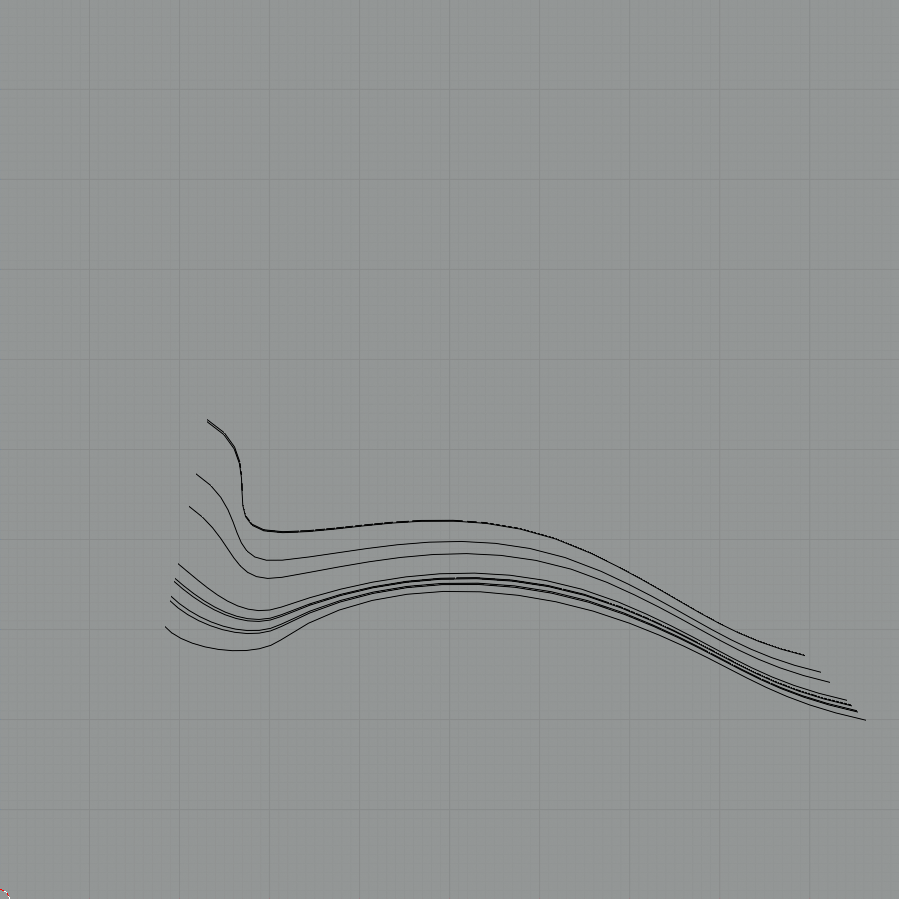
\includegraphics[width=0.3\textwidth]{graphics/0wings_withoutAdditionalVariance.png}}
  \qquad
  \subfloat[$0$ Flügel, mit Anpassung]{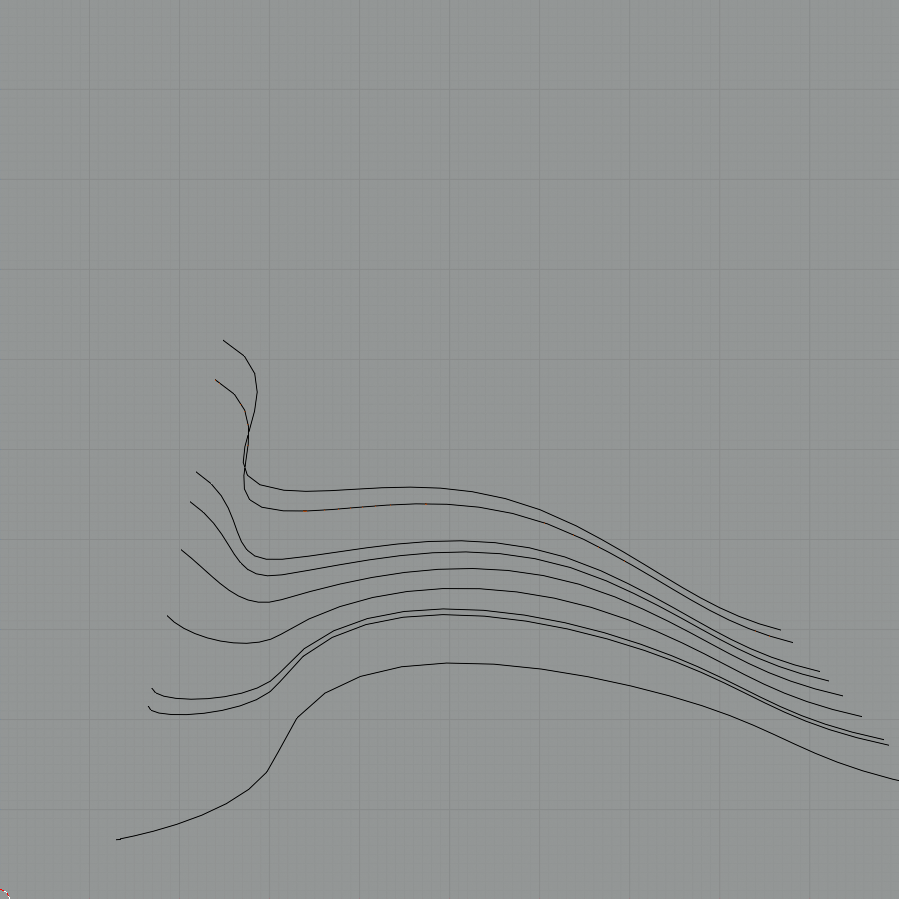
\includegraphics[width=0.3\textwidth]{graphics/0wings_withAdditionalVariance.png}}
  \qquad
  \subfloat[$1$ Paar Beine, mit Anpassung]{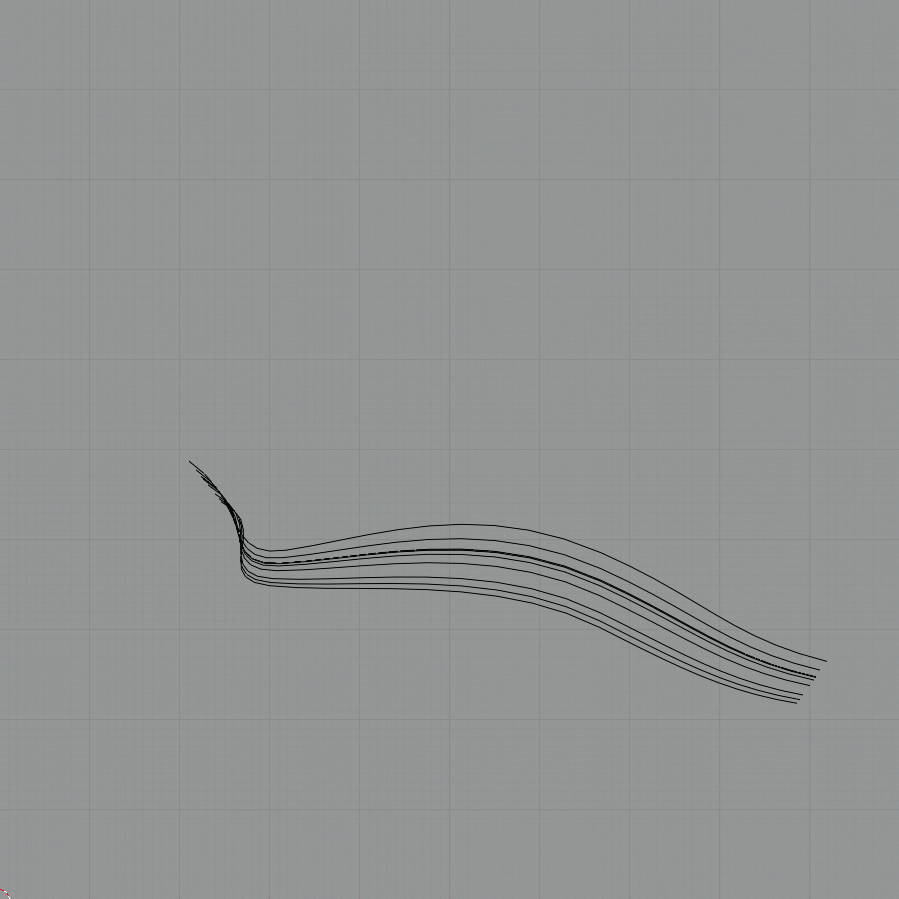
\includegraphics[width=0.3\textwidth]{graphics/1leg_withAdditionalVariance.png}}
  
  \caption{Jeweils $10$ bedingt zufällig generierte Wirbelsäulen. (a) und (b) ohne Flügel, (c) mit einem Paar Beine. In (b) und (c) wird ein zufälliger Wert aus $[-0.5, 0.5]$ auf die Bedingung (Flügel $= 0$ \bzw Beine $= 1$) aufaddiert.}
  \label{spine_variance}
 \end{figure}

 
 % Übergang Krokodil -> Fisch
 Schaut man sich nun die erzeugten Wirbelsäulen mit einem Paar tragender Beine an (Abbildung \ref{spine_variance}c), so liegen sie alle recht nah an der mittleren Wirbelsäule (Abbildung \ref{mean}).
 Das wirkt zunächst überraschend, da die meisten Tiere in den erhobenen Beispielen, die zwei Beine haben, Vögel sind. Sie haben eine Wirbelsäule, die hoch über dem Boden liegt und relativ aufrecht ist. Dann gibt es noch Känguru und Tyrannosaurus Rex. Bei ihnen liegt die Wirbelsäule ähnlich. Es muss aber auch einen Übergang von bodennahen Vierbeinern wie Krokodilen oder Fröschen über Zweibeiner zu Fischen ohne Beine geben. Nur gibt es dafür in der Natur eher wenige Beispiele. In den erhobenen Daten sind das nur der Seehund und die Ohrenrobbe.
 
 % Bedingungen an abgeleitet Werte
 Nun möchte man vielleicht Bedingungen an das zu generierende Skelett stellen, die nicht schon genau so in den erhobenen Daten repräsentiert sind. 
 Bedingungen an Dimensionen, die gar nicht erhoben wurden, können  entweder, unabhängig von der PCA, in den Ersetzungsregeln erzwungen werden, wie \zb die Anzahl der Flossen, oder sie müssen in die Erhebung eingefügt werden.
 
 Bedingungen, die schon implizit in den erhobenen Daten enthalten sind, sind beispielsweise die Schwanz- oder Halslänge. Um an sie Bedingungen stellen zu können, könnte man ebenfalls eine zusätzliche Dimension einfügen. Sie kann einfach aus den schon bestehenden Dimensionen errechnet werden. Dabei wäre aber das Problem, dass nur die Dimensionalität der Daten erhöht wird, nicht aber die eingegebenen Informationen. Es wären also mehr Eingabebeispiele nötig, nur dafür, dass die PCA eine offensichtliche Korrelation der Dimensionen erkennt.
 
 Die bessere Alternative ist die Eingabedimensionen der PCA umzuparametrisieren. Die Länge des Schwanzes in x-Richtung, ist \zb implizit in der Differenz der x-Koordinaten des ersten und letzten Kontrollpunktes der Bezièrkurve des Schwanzes enthalten. Ersetzt man nun den absoluten x-Wert des letzten Kontrollpunktes durch den Abstand in x-Richtung zum ersten Kontrollpunkt, so lässt sich die Schwanzlänge in x-Richtung ganz einfach als Bedingung an die PCA stellen. 
 
 % Schwanzlänge messen
 Betrachtet man nun konkret den Wunsch die Schwanzlänge festzulegen, ist das nicht ganz so einfach. Die Längen in x- und y-Richtung lassen sich zwar leicht festlegen, diese Längen sagen aber im Allgemeinen noch nicht viel über die tatsächliche Länge der Bezièrkurve aus. Verlangt man \zb eine Länge von $0$px für den Schwanz in x-Richtung, so haben die generierten Datenpunkte einen Schwanz der zwar auf gleicher Höhe beginnt und endet, aber trotzdem vorhanden ist und einen kleinen Bogen beschreibt. \todo{Beispielbild}
 Um die wirkliche Länge des Schwanzes zu messen, müsste man also noch mehr Aufwand in die Umparametrisierung stecken oder doch eine zusätzliche Dimension für die PCA in Kauf nehmen.
 
 

%---------------------------------------------------------------
%---------------------------------------------------------------
\chapter{Erzeugung eines Skeletts}
\label{chapter:non_pca_things}

%--------------------------------------------------
\section{Überblick über den Ablauf der Generierung}

\todo{Überblick über den Ablauf des Algorithmus}\\
\todo{"`Kommunikation"' über SkeletonGenerator}

\begin{itemize}
 \item Einheiten der PCA für Koordinaten $[0, 1000]$, deshalb sind die Wirbelsäulen der generierten Skelette auch in diesem Rahmen. Blender interpretiert eine Einheit als $1$m. Deshalb wirken sie sehr groß.
 
 \item Die Abmessungen der Knochen in die verschiedenen Richtungen ist bei den meisten Knochen relativ beliebig gewählt und oft auch immer gleich (außer bei Längen, die von PCA vorgegeben sind). Dafür gibt es keine biologische oder anatomische Grundlage. Man könnte hier sicherlich noch mehr machen (mehr Zufall, mehr anatomisch korrekt etc.)
 \todo{in Implementierungsdetails aufzählen was an Abmessungen alles beliebig (oder auch weniger beliebig) festgelegt wurde.}
\end{itemize}

%-----------------------------------------------
\section{Extremitäten}
\label{section:extremity_generation}

Ein Punkt im PCA-Raum gibt schon viele Eigenschaften des zu generierenden Skeletts vor. Zu den Dingen, die noch festgelegt werden müssen, zählen \zb die Anzahl und Anordnung der Wirbel und Rippen und vor allem die Ausrichtung der Extremitäten.

% Allgemeine Schwierigkeit Extremitäten zu positionieren
Das Skelett soll in einer Art Ruheposition dargestellt werden. Im Allgemeinen ist aber nicht klar wie die Ruheposition einer Extremität aussieht. Das ist schon allein daran zu erkennen, dass auf Darstellungen von Wirbeltierskeletten Flügel manchmal ausgestreckt und manchmal eingefaltet sind. Auch Beine sind meist so angeordnet, dass es aussieht als würde das entsprechende Tier gerade laufen. Dies ist auf Abbildung \ref{klippschliefer} am Beispiel des Klippschliefers sehr gut zu sehen.

 \begin{figure}
  \centering
  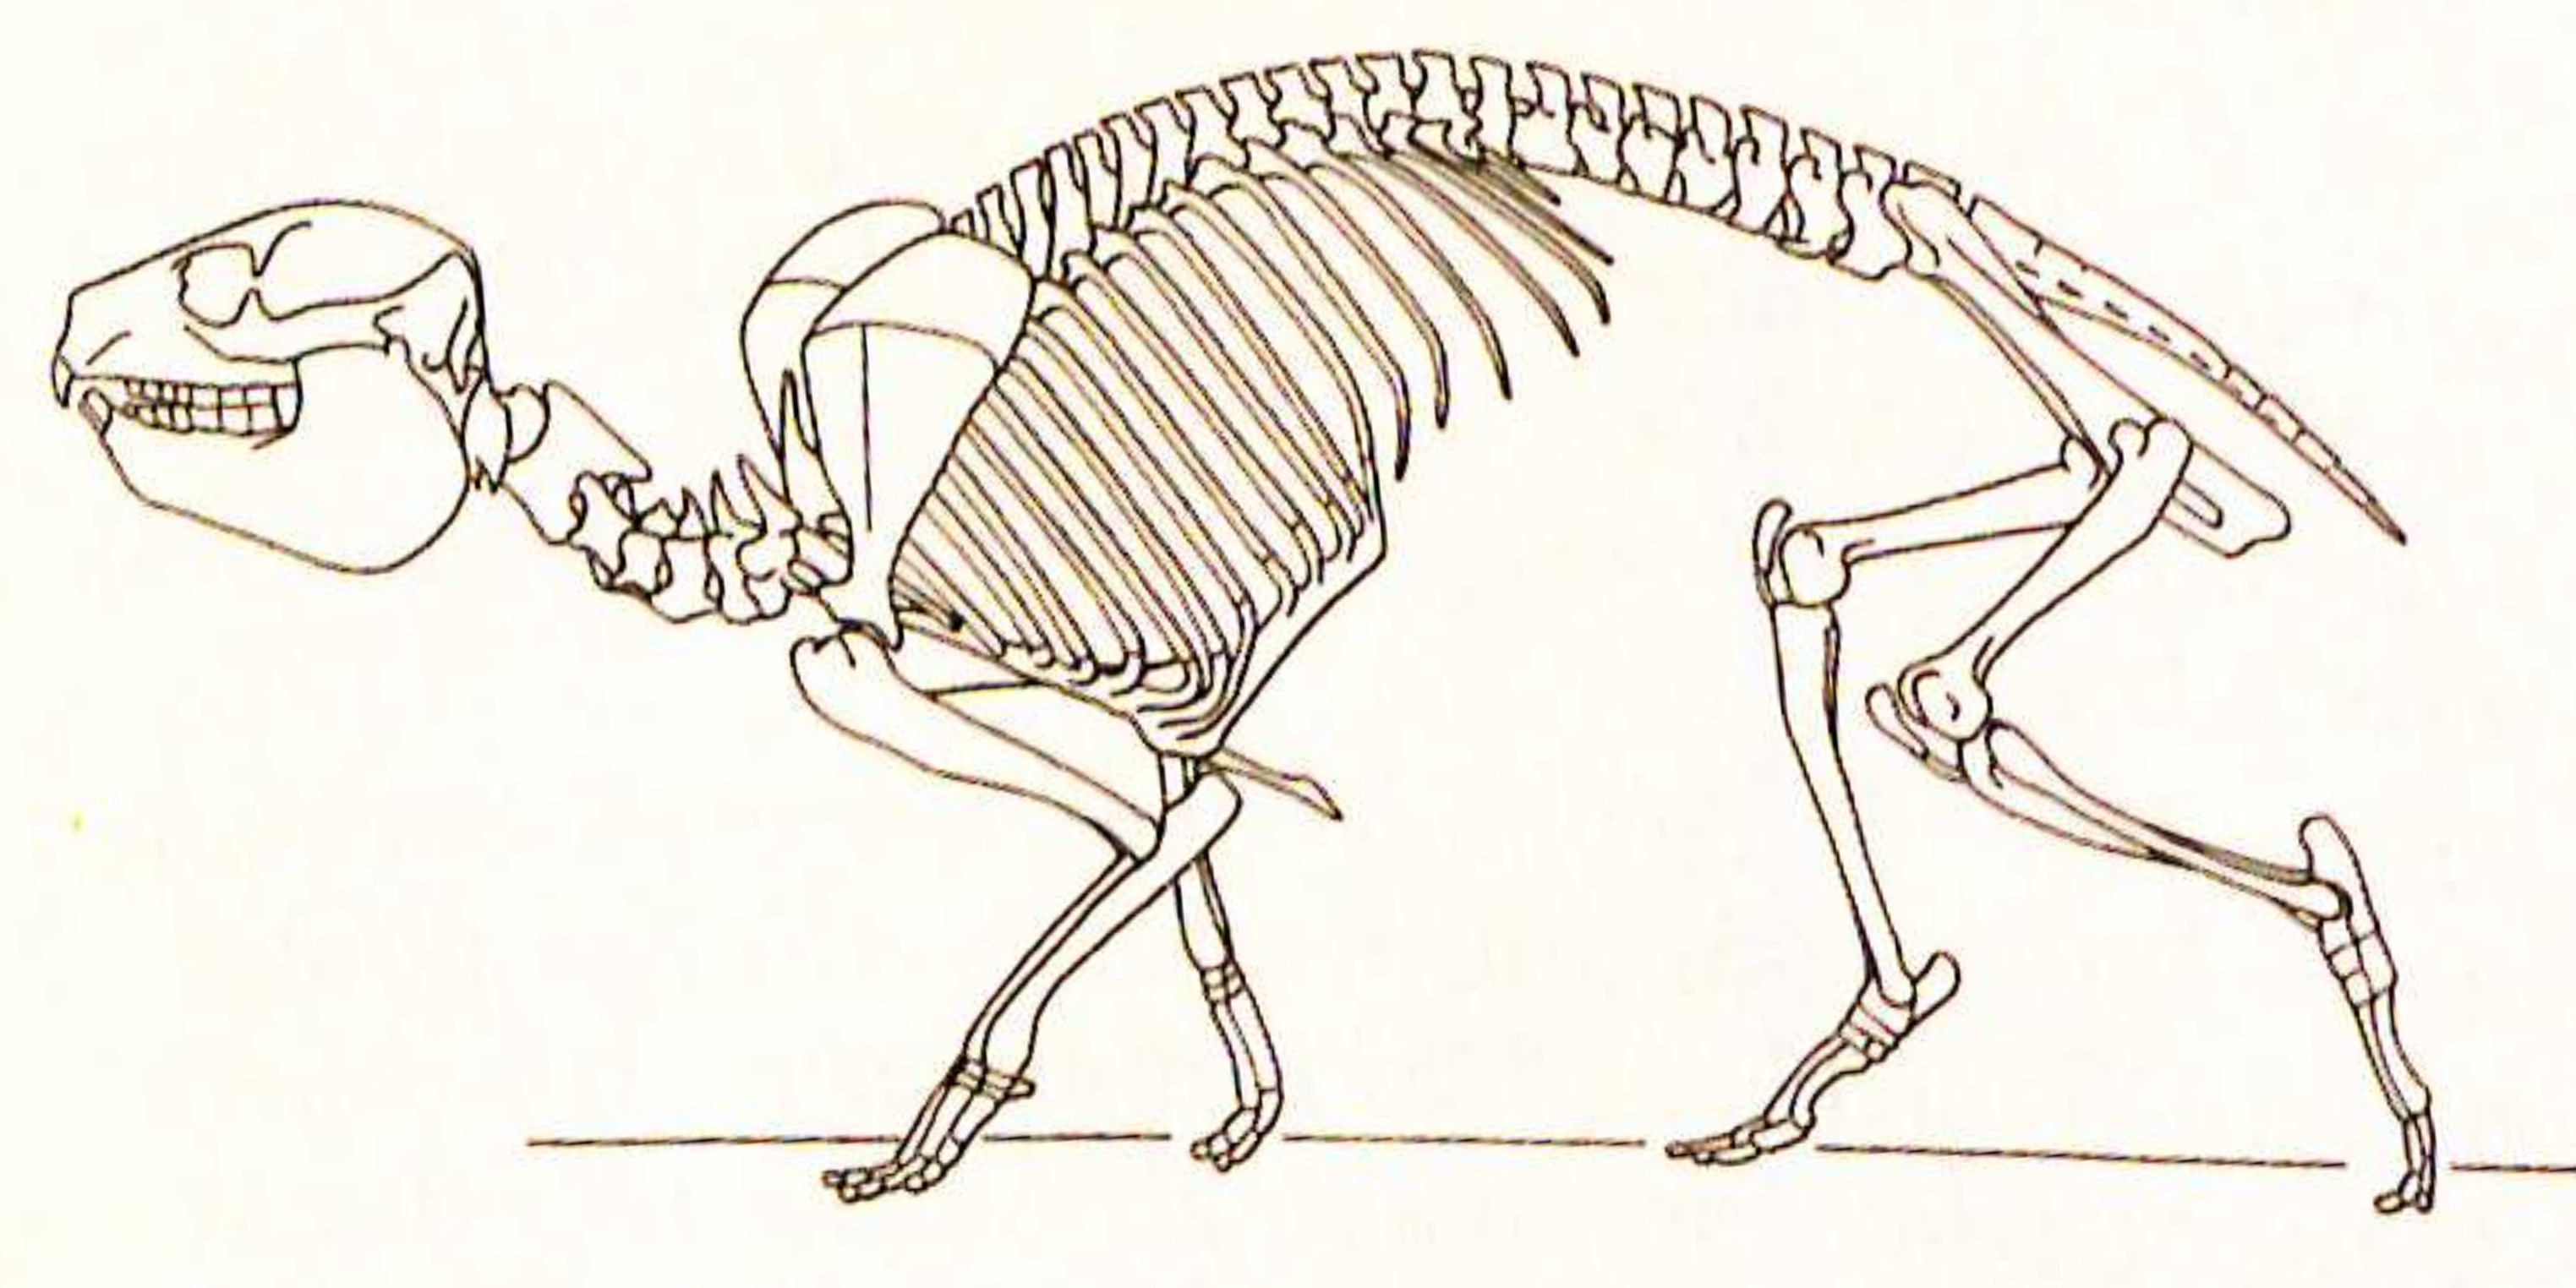
\includegraphics{../PCA/Skelettbilder/Klippschliefer.jpg}
  \caption{Skelett eines Klippschliefers. Dieses Bild wurde auch als Eingabe für die PCA verwendet.}
  \label{klippschliefer}
 \end{figure}

Wie in Kapitel \ref{chapter:pca} zur PCA schon erwähnt, ist es deshalb auch schwer möglich die Ausrichtung der Extremitäten \bzw die Winkel an den Gelenken als zusätzliche Dimension in den PCA-Raum mitaufzunehmen.

Die Positionierung der Extremitäten bleibt also ein Problem mit unklaren Anforderungen und vielen Freiheitsgraden.

% Einteilung in Kategorien
Ein erster Schritt an das Problem heranzugehen, ist es in kleinere Unterprobleme zu zerteilen.
Extremitäten können anhand ihrer Funktion in vier Kategorien eingeteilt werden:
Flügel, Flossen, Extremitäten mit Bodenkontakt (im Folgenden als Beine bezeichnet), und Extremitäten ohne Bodenkontakt (im Folgenden als Arme bezeichnet).

Für Flügel, Flossen und Arme gibt es keine besonderen Anforderungen außer, dass sie als solche zu erkennen sein sollten. Deshalb werden sie nach folgenden simplen Anweisungen orientiert:
\todo{Beispielbilder?}
\begin{itemize}
 \item Flossen: Ausrichtung gerade nach hinten (orientiert an Welt-x-Achse)
 \item Arme: Der Oberarm zeigt senkrecht nach unten (orientiert an Welt-y-Achse), im Ellenbogengelenk ist ein $90^{\circ}$ Winkel und die Hand verlängert Unterarm nach vorne.
 \item Flügel: Jedes beteiligte Gelenk hat ein Intervall mit festen Grenzen speziell für Flügel, aus dem zufällig ein Winkel gewählt wird.
\end{itemize}

Nun bleibt nur doch die Ausrichtung der Beine, für die die zusätzliche Anforderung gilt, dass sie den Boden berühren sollen.


%- - - - - - - - - - - - - - - - - - 
\subsection{Berechnung der Bodenhöhe}
\label{floor_height}

% Warum nicht Höhe 0?
Zunächst könnte man davon ausgehen, dass der Boden einfach auf Höhe null sein sollte. Das Problem hierbei ist aber, dass die von der PCA berechneten Längen für die Extremitäten meist so kurz sind, dass die Beine dann den Boden nicht mehr erreichen würden. Das liegt daran, dass auf den Bildern, die als Eingabebeispiele für die PCA verwendet wurden, der Boden meistens nicht ganz am unteren Rand ist. Hier würde rigoroses Abschneiden der Bilder auf Fußhöhe wahrscheinlich helfen, es würde in vielen Fällen aber auch ein Großteil der Füße verloren gehen.

% Berechnung
Die Höhe des Bodens wird also anhand der von der PCA generierten Längen der Extremitäten festgelegt.
Theoretisch würde es reichen einfach das kürzeste Bein im komplett ausgestreckten Zustand zu betrachten und den Boden auf die Höhe dessen Endpunkts festzulegen.
Das führt aber zu unnatürlich aussehenden Beinen, da das kürzeste Bein dann genau senkrecht nach unten führen muss um den Boden zu erreichen.

Deshalb wird nur ein bestimmter Anteil der Länge der Beine betrachtet. So wird erzwungen, dass die Beine, wenn sie auf dem neu definierten Boden stehen, auch etwas gekrümmt sind. Dieser Anteil ist in der Implementierung mit $0.8$ festgelegt, lässt sich aber natürlich auch variieren.

Wie in Kapitel \ref{chapter:biology} beschreiben gibt es verschiedene Arten von Füßen. Die oben beschriebene Berechnung geht davon aus, dass der Boden mit der Fußspitze berührt wird. Aber natürlich gibt es auch Wirbeltiere, die mit dem flachen Fuß auf der Erde stehen.
Deshalb wird zusätzlich zur Bodenhöhe noch eine Wahrscheinlichkeit berechnet, dass Verse \bzw Handgelenk den Boden berühren.

Wird die Bodenhöhe nach oben verschoben, weil die Beine insgesamt zu kurz sind, ist diese Wahrscheinlichkeit null.
Sind die Beine so lang, dass schon ohne die Bodenhöhe anzupassen die Verse \bzw das Handgelenk auf den Boden reicht, so ist sie eins.
Ansonsten ist die Wahrscheinlichkeit 
\[\frac{\text{Beinlänge} - \text{Höhe des Extremitätengürtels über }0}{\text{Länge des Fußes}}\]
Wenn es Vorder- und Hinterbeine gibt, so wird für beide diese Wahrscheinlichkeit berechnet und dann der Mittelwert genommen. Denn es ist sinnvoll, dass alle Beine den gleichen Punkt auf den Boden bringen.
Deshalb legt auch das erste Bein, das generiert wird, basierend auf der oben berechneten Wahrscheinlichkeit, fest, welcher Punkt gewählt wird.


%- - - - - - - - - - - - - - - - - - - - - - - - -
\subsection{Algorithmus zur Ausrichtung der Beine}
\label{leg_algo}

Eine Herangehensweise dieses Problem zu lösen, wäre inverse Kinematik zu verwenden. Dieses Verfahren wird unter anderem in der Robotik verwendet. Gegeben ist eine Kette von Gelenken, die über starre Verbindungsteile miteinander verbunden sind. Für ein oder mehrere Punkte auf dieser Kette können Zielpunkte im Raum angegeben werden. Das Ziel ist es dann eine Konfiguration der Gelenke zu berechnen, so dass alle Zielpunkte erreicht werden.\\
Es gibt viele verschiedene Methoden Probleme aus der inversen Kinematik zu lösen. Diese finden jeweils in Abhängigkeit von der konkreten Problemstellung ihre Anwendung. Ein Überblick über die verschiedenen Techniken ist in Zusammenstellung \cite{IKSurvey} zu finden.

Da das vorliegende Problem aber recht viele Randbedingungen hat, die ausgenutzt werden können, ist es gar nicht unbedingt nötig einen schwergewichtigen Algorithmus zu implementieren, der ein allgemeineres Problem löst.\\
Hier ist \zb in den allermeisten Fällen klar in welche Richtung ein Gelenk gedreht werden muss um den Fuß dem Boden zu nähern oder ihn vom Boden zu entfernen. Außerdem ist gar kein spezieller Punkt auf dem Boden vorgegeben, der erreicht werden soll.

Deshalb wurde hier ein eigener, recht simpler Algorithmus entwickelt, der auf dieses spezielle Problem angepasst ist.


% \begin{algorithm}
%  \caption{Beinalgorithmus}
%  \label{beinalgo}
%  
%  \begin{algorithmic}
%     \STATE{step = 0\\
%     maxSteps = 50\\
%     angleStepSize = $40^\circ$}
% 
%     \WHILE{floor not reached and step < maxSteps}
%         \FORALL{joints}
%             \IF{child bone of joint has not reached floor and movement nearer to floor possible}
%                 \STATE try change joint angle
%             \ENDIF
%         \ENDFOR
%         \IF{angleStepSize > eps}
%             \STATE reduce angleStepSize
%         \ENDIF
%     \ENDWHILE
%  \end{algorithmic}
% \end{algorithm}
\todo{Pseudocode?}

% iterativ, Drehrichtung
Der Algorithmus geht iterativ vor.
In jedem Schritt wird für jedes Gelenk berechnet ob sein Winkel vergrößert oder verkleinert werden muss um den dazugehörigen Knochen näher zum Boden zu bewegen.
Mit dem "`dazugehörigen"' Knochen ist hier derjenige der beiden an das Gelenk anschließenden Knochen gemeint, der das Kindelement des anderen ist.
Die Drehrichtung lässt sich relativ leicht herausfinden indem die Ausrichtung des Knochens mit der Welt-y-Achse verglichen wird. Je senkrechter der Knochen ausgerichtet ist, desto ausgestreckter ist das Bein.

% Einschränkungen der Gelenke
Zusätzlich gibt es für jedes Gelenk und jeden Freiheitsgrad einen minimalen und einen maximalen Winkel, der eingenommen werden kann. Dieses Intervall hängt von den anatomischen Möglichkeiten des Gelenks ab und von den Winkeln, die in einer "`sinnvollen"' Ruheposition eingenommen werden können. 
\todo{ist das überhaupt eine Einschränkung?}
Es gibt also lokale Einschränkungen je nach Gelenk und globale Randbedingungen. % Problematik mit lokalen Winkelkonstraints vs. globalen Berechnungen für Abstand zum Boden?

% Startposition, Bewegungseinschränkungen
Die Startposition der Extremität ist maximal angewinkelt. Die Gelenke beginnen also mit ihren kleinst- \bzw größtmöglichen Winkeln. In den folgenden Iterationen wird dann derjenige Endpunkt der Extremität dem Boden genähert, der zum Schluss Bodenkontakt haben soll. \todo{würde wahrscheinlich auch mit ausgestrecktem Bein als Startpos gehen; was wäre dabei zu beachten}
Ohne weitere Einschränkungen kann es nun passieren, dass unnatürliche Positionen auftreten, in denen \zb der Fußspann näher am Boden ist als die Fußsohle.
Oder es kann passieren, dass ein Knochen über die positive Welt-y-Achse hinaus gedreht wird. Das Problem dabei ist, dass die Einschränkungen an den Gelenken nicht zulassen, dass der Knochen sich unbegrenzt in diese Richtung weiterdreht und der Knochen dann "`feststeckt"'. Deshalb wird nach jeder Drehung festgestellt ob so eine Situation eingetreten ist und wenn ja, wird die Drehung rückgängig gemacht.
Die Drehung wird ebenfalls rückgängig gemacht, falls sie bewirkt, dass die Knochen unterhalb der Bodenhöhe landen.
\todo{Beispielbilder}
So ist zu jeder Zeit garantiert, dass die Knochen auf der "`richtigen"' Seite der y-Achse liegen und nicht unterhalb der Bodenhöhe sind. % Invarianten

% Verkleinerung der Größe der Drehwinkel
In jeder Iteration werden die Winkel, um den die Gelenke gedreht werden, um einen bestimmten Anteil verkleinert. Zu Beginn soll, mit großen Veränderungen, eine grobe Ausrichtung der Gelenke vorgenommen werden, die dann immer weiter verfeinert wird.
Der Startwinkel darf nicht zu klein sein, weil die Gelenke sonst ihre Zielpositionen nicht erreichen können. Ist der Startwinkel allerdings zu groß, bewirkt es in vielen Fällen nur, dass die Drehung nicht durchgeführt werden kann, weil die oben genannten Randbedingungen verletzt werden.\\
Die Verkleinerung des Winkels darf nicht zu schnell geschehen, weil dann wiederum die Endposition nicht erreicht werden kann. Wenn sie aber zu langsam geschieht passiert in vielen Schritten wiederum nichts wegen verletzter Randbedingungen.\\
Durch Ausprobieren wurden folgende Zahlen als sinnvoll erachtet: Startwinkel $40^{\circ}$, später dann jeweils $\frac{6}{7}$ davon.

Falls sich der Abstand zum Boden kaum verändert, liegt also die Vermutung nahe, dass die Gradzahl zu groß ist und deshalb alle möglichen Winkeländerungen invalide sind. Deshalb wird in diesem Fall die Gradzahl für die nächste Iteration stärker verkleinert (halbiert).

\todo{Wkten für Gelenke, Vorteil?}

% Zweiter Freiheitsgrad
Theoretisch haben das Hüft- und das Schultergelenk nicht nur einen, sonder zwei Freiheitsgrade. Der Oberschenkel lässt sich nicht nur nach vorne und hinten bewegen, sondern auch seitlich abspreizen. Das lässt sich auch leicht als zweite Art von Gelenk im Code abbilden. Allerdings liefert der Algorithmus dann oft seltsam anmutende breitbeinige Tiere.
Deshalb wurde der zweite Freiheitsgrad hier außen vor gelassen.
Obwohl es natürlich in der Natur auch viele Tiere mit nach außen gestellten Beinen gibt, wie \zb Echsen.
% + max angewinkelte Pos komisch und Drehrichtung ändert sich je nach anderen Winkel

% Probleme bei sehr kurzen Beinen
Treten sehr kurzen Beinen auf, hat der Algorithmus außerdem einige kleine Probleme. Diese werden genauer in Abschnitt \ref{leg_positioning_short_legs} beschrieben. Da die Beine aber in diesen Fällen, wie gesagt, sehr kurz sind, ist es für den Gesamteindruck gar nicht besonders wichtig wie genau sie angeordnet sind.

% Vergleich echter und generierter Beinstellungen
Wie in Kapitel \ref{chapter:additional_features} beschrieben, lassen sich auch die Eingabebeispiele der PCA laden. Bei ihnen sind dann alle Attribute, die die PCA liefert, schon festgelegt. Alle anderen müssen jedoch noch generiert werden.
Dazu gehören auch die Beine.
Vergleicht man nun die Beinstellung, die der oben beschriebene Algorithmus generiert, mit der Beinstellung auf dem Eingabebild, lassen sich teilweise sehr große Unterschiede feststellen. \todo{gutes und schlechtes Beispiel (schlecht: Brachiosaurus, Elefant)}

% Mehr Infos nötig für Verbesserungen
Um in allen Fällen eine realistisch wirkende Positionierung der Beine zu bekommen, müsste noch sehr viel mehr Arbeit in den Algorithmus gesteckt werden. Außerdem bräuchte der Algorithmus mehr Informationen zum Tier. Solche Zusatzinformationen könnten beispielsweise die Art des Fußes oder die Fortbewegungsart sein. Auch könnte es helfen, wenn es eine sinnvolle Möglichkeit gäbe die Winkel an den Gelenken als Dimension für die PCA mitaufzunehmen. Dafür müsste man sich aber, wie zu Beginn des Kapitels schon erwähnt, auf eine kanonische Ruheposition einigen und dann auch noch Beispiele in genau dieser Position finden.

% für Weiterverwendung werden Beine sowieso angepasst
Ein fertig generiertes Skelett wird höchstwahrscheinlich auch noch "`weiterverarbeitet"'. Soll \zb ein animiertes Tier daraus werden, so müssen Bewegungszyklen geschaffen werden. Dafür muss jedes Gelenk vielfach bewegt werden. Soll ein Tier mit Haut und Muskeln daraus werden, so müssen Muskeln an den Knochen ansetzen, die dann einen nicht unerheblichen Anteil an der Positionierung der Beine haben.

% Beinalgo nicht weiter anpassen
Die von dem hier beschriebenen Algorithmus generierte Position kann also gut als erster Eindruck dienen muss aber in den meisten Fällen noch angepasst werden. Ausgehend von der gegebenen Datenlagen und von den zu erwartenden Anwendungen ist es aber nicht sinnvoll den Algorithmus weiter zu verfeinern.

%--------------------------------------
\subsection{Zusätzliche Ansatzpunkte für Extremitäten}

Ansatzpunkte für Extremitäten sind natürlich zunächst der Hüftgürtel und der Schultergürtel. Um auch die Generierung fantastischer Tiere zu ermöglichen, ist es aber möglich dies zu erweitern.

% 2 Extremitäten an einem Gürtel
Eine einfache Möglichkeit ist hier zunächst die Anzahl der möglichen Extremitätenpaare von zwei auf vier zu erhöhen, indem einfach an der Hüfte und der Schulter jeweils zwei Paare ansetzen dürfen. Dafür wurden an der Hüfte \bzw der Schulter mehrere Gelenke direkt hintereinander angelegt, an denen Extremitäten ansetzen können.\\
% Keine Flügel und Arme an der Hüfte
Flügel und Arme dürfen hierbei weiterhin nur an der Schulter ansetzen, Beine und Flossen an beiden Stellen. Der Grund dafür ist, dass die meisten generierten Skelette seltsam wirken, wenn an der Hüfte Flügel oder Arme ansetzen und dafür an der Schulter Beine beginnen. Das liegt daran, dass existierende Tiere mit Flügeln oder Armen ihren Schwerpunkt im hinteren Bereich haben und sie auf den Hinterbeinen stehen. Deshalb wird die Wirbelsäule durch die PCA auch dementsprechend angelegt.

% mehr Extremitätengürtel auf dem Rücken
Eine Überlegung war auch zwischen Schulter und Hüfte weitere Extremitätengürtel anzubringen. Das stellt sich aber als schwierig heraus. Die Wirbelsäule ist zwischen Hüfte und Schulter nach oben geschwungen und im Bauchraum befinden sich die meisten Organe des Tieres. Ein zusätzlicher Extremitätengürtel würde den Bauchraum einschränken. Außerdem wirkt dann auch die nach oben geschwungene Wirbelsäule anatomisch seltsam.
"`Verdoppelt"' man die Schwingung der Wirbelsäule und hängt einfach einen weiteren Rücken hinten oder vorne an, so wirkt es ebenso seltsam, da dann die "`Höcker"' der Wirbelsäule für das Tier wahrscheinlich nicht wirklich ein Vorteil sind und nur die Fortbewegung erschweren.

% zweiter Schultergürtel
Eine weitere Idee, die auch umgesetzt wurde, ist, eine Art Zentauren zu ermöglichen. Hat das Tier einen Hals, der lang genug ist, kann darauf ein weiterer Schultergürtel kurz unterhalb vom Kopf angebracht werden. An diesem Schultergürtel dürfen dann alle Arten von Extremitäten außer Beinen ansetzen. Das wirkt tatsächlich meist auch anatomisch einigermaßen sinnvoll.\\
Ein solcher Schultergürtel wirkt aber nur sinnvoll, wenn auch der Hals lang genug ist. Deshalb wird die Benutzereingabe, die einen zweiten Schultergürtel erzwingt in eine Bedingung für die Halslänge umgewandelt und an die PCA weitergegeben. Gibt es keine Benutzereingabe, so wird ein zweiter Schultergürtel nur generiert, wenn der Hals lang genug ist.

%----------------------------------- 
\subsection{Anordnung und Anzahl der Extremitäten}

Ein PCA-Datenpunkt stellt die Länge der Vorder- und Hinterbeine, die Wahrscheinlichkeit für Flügel und die "`Wahrscheinlichkeit"' für Beine zur Verfügung.
Die genaue Anzahl (auch für fantastische Tiere) und die Anordnung müssen noch festgelegt werden.

Die Position jeder Extremität wird zufällig aus der Menge der möglichen Positionen gewählt. Beine dürfen nicht am zusätzlichen Schultergürtel am Hals generiert werden, Arme und Flügel dürfen nicht an der Hüfte generiert werden und Flossen sind überall erlaubt.\\
Ist für eine Extremität kein Platz mehr, wird zunächst getestet, ob eine der anderen Extremitäten an ihre Position wechseln kann um Platz zu schaffen. Erst wenn das fehlschlägt kann die betreffende Extremität nicht platziert werden.\\
Da die Positionen nicht deterministisch gewählt werden, kommt es bei Tieren mit mehreren möglichen Anordnungen zu unterschiedlichen Ergebnissen bei gleicher Eingabe.

Die Anzahl und Art der Extremitäten orientiert sich zunächst an Benutzereingabe. Gegebenenfalls wurden diese Eingaben auch schon als Bedingungen an die PCA weitergeleitet (siehe Abschnitt \ref{pca_conditions}).

Falls es keine Benutzereingabe für eine Art von Extremitäten gibt, so wird zunächst getestet ob es noch Platz gibt für diese Art. Falls noch Platz vorhanden ist, wird je nach Art unterschiedlich vorgegangen:
Die Anzahl der Beine oder Flügel wird anhand der Wahrscheinlichkeiten des PCA-Datenpunktes generiert, aber maximal ein Paar pro Schulter- und Hüftgürtel. Die "`Wahrscheinlichkeit"' der Beine liegt im Intervall $[0, 2]$. Hier wird, je nach dem ob die "`Wahrscheinlichkeit"' in $[0, 1]$ oder in $[1, 2]$ liegt, ausgelost ob null oder ein \bzw ein oder zwei Beinpaare generiert werden.\\
Für Arme und Flossen gibt es keine Anhaltspunkte durch die PCA. Deshalb wurde einfach festgelegt, dass Arme, wie Flügel, mit der PCA-Flügelwahrscheinlichkeit generiert werden. Beine werden ganz zum Schluss in noch komplett leeren Extremitätengürteln generiert, falls die Länge der dort zu generierenden Extremitäten nicht zu lang ist.

\todo{nachträgliche Umverteilung der Extremitäten sinnvoll? (leere Gürtel auffüllen)}

Dieses Vorgehen führt dazu, dass, wenn ein PCA-Beispiel geladen wird, die Anzahl, Art und Position der Extremitäten nicht unbedingt dem realen Tier entsprechen muss.
Zunächst kann es einen zusätzlichen Schultergürtel geben, falls der Nutzer das erlaubt und der Hals lang genug ist, und es können mehrere Extremitäten pro Extremitätengürtel platziert werden, wenn das erlaubt ist.\\
Die Anzahl der Flügel und Beine wird stimmen, da ihre Wahrscheinlichkeiten ja festgelegt sind, aber ihre Position wird zufällig bestimmt, falls möglich.  Arme und Flossen werden nach den oben genannten Kriterien generiert, falls der Nutzer nichts anderes vorgibt.\\
Wenn ein Tier also möglichst genau reproduziert werden soll, sollte zumindest die Anzahl der Arme und Flossen angegeben werden und ein zweiter Schultergürtel und mehrere Extremitäten pro Gürtel verboten werden.


%---------------------------------------------------
\section{Wirbel und Rippen}

Weitere Dinge, die festgelegt werden müssen, ist die Anzahl der Wirbel auf den einzelnen Teilen der Wirbelsäule und die Anzahl der Rippen.

Die Anzahl der Wirbel orientiert sich an echten Wirbeltierskeletten (siehe Absatz \ref{biology_skeleton}). Auf dem Hals werden $7$ Wirbel generiert, außer das Tier hat Flügel, dann liegt die Anzahl zwischen $10$ und $30$. Auf dem Rücken liegen $25$ Wirbel und auf dem Schwanz $5$ bis $20$.

Eine Bézierkurve ist ein Weg im $\mathbb{R}^2$. Sie ist parametrisiert auf $[0, 1]$ und im Allgemeinen nicht nach Bogenlänge parametrisiert. Das heißt die Geschwindigkeit, mit der die Kurve durchlaufen wird, ist nicht konstant. Wertet man die Kurve also bei $0.5$ aus, wurde nicht notwendigerweise die Hälfte der Strecke zurückgelegt.\\
Für die Generierung von $n$ Wirbeln wurde die Kurve einfach an den Stellen $\frac{i}{n}$ ausgewertet, für $0 \leq i \leq n$. Durch den oben genannten Effekt variiert dann die Länge der Wirbel über den Kurvenverlauf.

Wird die Bézierkurve $B$ nach Bogenlänge umparametrisieren, so erhält man die Kurve $S$ mit:

\[S(t) = \int_0^t \| B'(s) \| ~\mathrm{d}s \]

Das obenstehende Integral ist jedoch schwer zu berechnen, da im Allgemeinen keine Stammfunktion des Integranden zur Verfügung steht. Es gibt jedoch numerische Methoden, mit denen das Problem gelöst werden kann. \cite{ArcLengthParametrization}

Betrachtet man echte Wirbeltiere, so sind keine einfachen Regeln für die Länge ihrer Wirbel ersichtlich. Es gibt beispielsweise eine Studie, die die Beschaffenheit der  Wirbel von Mäusen untersucht \cite{MouseVertebrae}. In dieser Studie auf Abbildung $5$, Seite $19$, ist sehr gut zu sehen, dass die Länge der Wirbel im Verlauf der Wirbelsäule sehr stark schwankt.



Die Anzahl der Rippen und auch die Ausdehnung des Brustkorbs variiert zwischen Wirbeltieren sehr stark. Es gibt Tiere, die an jedem Wirbel der Rückenwirbelsäule Rippen haben und es gibt Tiere die haben nur ein paar wenige auf dem vorderen Teil.
\todo{Beispiele}\\
Deshalb wird ein zufälliges Intervall $[0, x]$ auf der Bézierkurve des Rückens bestimmt. Jeder Wirbel, der in diesem Intervall liegt, bekommt auch eine Rippe.
\todo{Bestimmung der Rippenlänge beschreiben?}


%-----------------------
\section{Knochenmodelle}
\label{bone_models}

Zunächst wird jeder terminale Knochen durch seine Bounding Box dargestellt.
\todo{es sind nicht wirklich Bounding Boxen, eher "`Proxyboxen"'}
Diese Boxen lassen sich aber leicht durch die 3D-Modelle der entsprechenden Knochen ersetzen. Dazu müssen die 3D-Modelle nur im .obj-Format vorliegen und folgenden Bedingungen entsprechen:

Das Modell ist korrekt an den Achsen ausgerichtet und so verzerrt, dass es einen Würfel mit 1(m) Kantenlänge in jeder Richtung möglichst gut ausfüllt.

Lässt man es hierbei bewenden, so ist es relativ schwierig herauszufinden wie man die einzelnen Knochen skalieren muss, dass sie an den Gelenken gut zusammenpassen. Außerdem ist es aufwändig herauszufinden wo die Gelenke an den Knochen ansetzen.

Setzt man sich dagegen etwas über den Gedanken der "`Bounding Box"' hinweg, so kann die Positionierung und Skalierung einfacher werden. Hier wurden, je nach Knochen, einige der folgenden Punkte umgesetzt. \todo{Beispielbilder}
\begin{itemize}
 \item Kleine Fortsätze, die nicht wirklich zur (optischen) Größe des Knochens beitragen, \zb die Fortsätze der Wirbel, ragen aus der Bounding Box heraus.
 
 \item Kantenlängen, die von "`außen"' vorgegeben werden, sind genau auf die Kantenlänge der Box skaliert (also 1). So beispielsweise die x-Länge der Wirbel, die auf der Wirbelsäule genau aneinender stoßen sollen. Dies können aber auch Längen sein, nur einen Teil des Knochens betreffen. Der Beinabstand an der Hüfte ist \zb kleiner als die komplette Breite der Hüfte. Es ist aber einfacher den Beinabstand anzugeben, als die Hüftbreite. Auch die Skalierung der Hüfte in x-Richtung ist zunächst nicht klar, aber wenn die Breite der zugehörigen Wirbel gegeben ist, ist auch klar, wie breit die Hüfte sein soll. Deshalb ist die Hüfte in x-Richtung so skaliert, dass der Teil, an dem der Wirbel ansetzt, schon die komplette Kantenlänge des Würfels ausfüllt. Bei Gelenken, die von der Breite her zusammenpassen sollen, ist dies auch sehr hilfreich. Aber das führt natürlich auch dazu, dass die "`Bounding Box"' nicht mehr viel mit der resultierenden Größe des Knochens zu tun haben muss.
 
 \item Kantenlängen, die nicht vorgegeben werden, sind einfacher passend zu bestimmen, wenn sie nicht komplett unabhängig von den anderen Raumrichtungen sind. Ist \zb die x- und y-Skalierung eines Knochens vorgegeben, und die Skalierung in z-Richtung soll nur möglichst gut dazu passen, so ist es sinnvoll, das 3D-Modell schon so zu speichern, dass die z-Richtung von einer der anderen Richtungen abhängt. Tut man dies nicht, so führt das relativ leicht dazu, dass die Knochen grundlos verzerrt werden.
 
 \item Längen die variiert werden können sollen \zb die Länge der Wirbel oder der Beinabstand der Hüfte sollten genau eine Kantenlänge der 1x1 Box einnehmen.
\end{itemize}
\todo{Schwierigkeit bei stark gebogenen Knochen}

Liegen die Modelle in diesem Format vor, können sie einfach eingelesen werden und anhand der Skalierung der Bounding Box skaliert werden.
Hier wurden vor allem Modelle von menschlichen Knochen verwendet, da sie leichter verfügbar sind. Manche Knochen sind jedoch auch von anderen Tieren. Das führt \zb bei dem verwendeten Unterarmknochen des Pferdes dazu, dass er etwas überdimensionierte Fortsätze am Ellenbogen bekommen, wenn man ihn großskaliert. Das liegt daran, dass dieser Knochen beim Pferd eigentlich relativ kurz ist.

% Ausrichtung der Knochen
Eine Schwierigkeit daran Modelle in der oben genannten Form herzustellen ist, dass nicht unbedingt sofort klar ist, wie die Knochen ausgerichtet werden müssen. Die Hüfte muss \zb so ausgerichtet werden, dass der Anfangs- und Endpunkt der durchgehenden Wirbelsäule auf gleicher Höhe liegen, damit nachfolgende Wirbel auch richtig anschließen. (Das funktioniert natürlich nur, weil die Wirbelsäule an der Stelle der Hüfte quasi gerade ist.) \todo{wg Lizenz Pferdehüfte verwendet, die nicht mit Wirbelsäule verwachsen ist}
Auch die Positionierung der Rippen und des Oberarms in Kombination mit dem Unterarm ist anspruchsvoll. Dabei hilft es 3D-Modelle zu haben, in denen die anderen Knochen auch schon vorhanden sind, um sich die Ausrichtung abzuschauen. Außerdem können Bilder von Skeletten zu Rate gezogen werden. Und zuletzt muss man die genaue Positionierung einfach testen.

% Gelenke korrekt ausrichten
Zusätzlich muss beachtet werden wie die Knochen aneinander anschließen \bzw wie sie für die entsprechenden Gelenke korrekt positioniert sind. Das erfordert etwas "`finetuning"'. Für jeden Knochen sind dafür in Abhängigkeit zur Bounding Box zwei Offsets gespeichert: das Offset zu dem Gelenk, das ihn mit seinem Elternknochen verbindet und das Offset zu dem Gelenk, das ihn mit seinem Kindknochen verbindet (oder mehrere, falls vorhanden). Dies sorgt dafür, dass die Positionierung der Knochen stimmt, egal wie groß sie sind. Ist ein Knochen sehr groß und ein anschließender sehr klein (oder anders herum), so kommt es natürlich trotzdem vor, dass die Gelenke nicht wirklich ineinander passen. Für solche Situationen bräuchte man verschiedene 3D-Modelle, die je nach Gegebenheit eingesetzt werden.

% Köpfe
% Köpfe sind kompliziert $\rightarrow$ Auswahl an Köpfen bereitstellen (evtl. leicht skalier-/verformbar oder ineinander überführbar)
Da der Kopf \bzw der Schädelknochen im Gegensatz zu anderen Knochen bei Wirbeltieren sehr stark variiert, ist es sinnvoll mehrere Schädelknochen zur Auswahl zu haben. Geht die Menge an verfügbaren Schädelknochen über "`Tier mit Flügeln"' und "`Tier ohne Flügel"' hinaus, so ist es außerdem sinnvoll die Auswahl des passenden Schädelknochens dem Nutzer zu überlassen.



% Hände und Füße
Bei Händen und Füßen ist das Problem ebenso, dass es sehr viele verschiedene Ausprägungen davon gibt. Hier lassen sie sich jedoch grob nach Extremitätentyp unterscheiden. Diese Unterscheidung kann aber beliebig fein sein. Hier wurde nur nach Flügel, Flosse \todo{?} und Extremität mit Bodenkontakt unterschieden. Und bei Extremitäten mit Bodenkontakt wurde nochmals danach unterschieden wie flach der Fuß oder die Hand auf dem Boden aufkommt (bei weniger als $45^\circ$ ist es eine menschliche Hand, sonst ein Huf). \todo{ggf. an Implementierung anpassen}
\todo{erwähnen, dass Knochen für Flügel"`hand"' nicht vollständig}

\todo{Schwanzspitze: ein Modell für drei Wirbel. Das sieht bei wenigen Wirbeln komisch abgeknickt aus}

% mehrere Extremitäten an einer Schulter/Hüfte
Setzten mehrere Extremitäten an einer Schulter oder einer Hüfte an, so ist ein "`normales"' Modell der Schulter/Hüfte nicht mehr ausreichend, da nicht genug Gelenke vorhanden sind. Dieses Problem wurde an der Schulter so behoben, dass einfach mehrere Schulterblätte mit einem gewissen Abstand generiert wurden. Für die Hüfte wurde ein kombiniertes 3D-Modell aus zwei einzelnen Hüften erstellt, an dem nun zwei Gelenke vorhanden sind.

\todo{3D-Modelle leider nicht ganz einfach Austauschbar wegen Offsets -> erkläre wie Offsets eingelesen werden müssten}
\todo{Wenn Muskeln generiert werden sollen, müssen noch mehr Ansatzpunkte bestimmt werden und Positionierung der Knochen hängt von Muskeln ab -> future work}




%-------------------------------
%-------------------------------
\chapter{Zusätzliche Funktionen}
\label{chapter:additional_features}

In Kapitel \ref{chapter:skeleton_generation} wird beschrieben wie der Algorithmus abläuft. In diesem Kapitel geht es nun darum die Verwendungsmöglichkeiten des Algorithmus auszuschöpfen. Über eine Benutzeroberfläche wird die Bedienung vereinfacht und gezeigt welche Möglichkeiten es gibt die Skelettgenerierung zu steuern. Außerdem ist es möglich die Metadaten eines Skeletts zu speichern und Variationen zu einem bestehenden Skelett zu generieren.


%---------------------------
\section{Benutzeroberfläche}
\label{gui}

Mit dem in Kapitel \ref{chapter:skeleton_generation} vorgestellten Algorithmus können nicht nur zufällige Skelette generiert werden. Über eine Benutzeroberfläche ist es auch möglich, dem Algorithmus zusätzliche Eingaben zu geben. Die Benutzeroberfläche ist in Abbildung \ref{gui_screenshot} zu sehen.

\begin{figure}
 \centering
 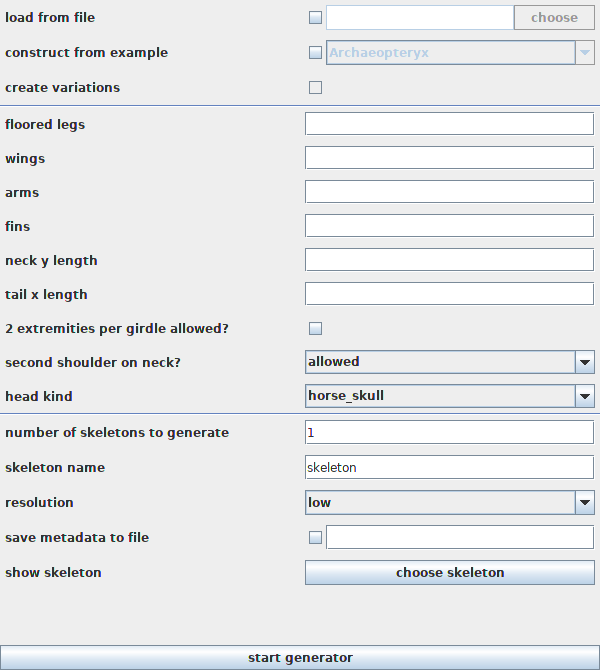
\includegraphics[width=0.7\textwidth]{graphics/gui.png}
 \caption{Die Benutzeroberfläche des Programms. Der Knopf "`start generator"' startet den Algorithmus mit den zusätzlichen Eingaben aus den Feldern darüber.}
 \label{gui_screenshot}
\end{figure}

Diese Eingaben werden unter anderem in Bedingungen umgewandelt, die schon von der PCA berücksichtigt werden. Wie eine bedingte Verteilung als Eingabe für die PCA berechnet wird, wird in Abschnitt \ref{pca_conditions} erklärt. Wie dort auch beschrieben, werden bei allen Bedingungen zufällige kleine Werte aufaddiert oder abgezogen um mehr Variation auf den erzeugten Skeletten zu bekommen. Dies ist sinnvoll, da der Benutzer so nicht gezwungen wird so etwas wie $1{,}4$ Beinpaare zu verlangen, um \zb die Form der Wirbelsäule zu verändern. Bei solch einer Eingabe müsste dann außerdem durch den Algorithmus ausgelost werden, ob das Skelett am Ende $1$ oder $2$ Beinpaare hat. Das wäre unter Umständen verwirrend.\\
Ist in Zahlenfeldern nichts eingegeben, haben diese keinen Einfluss auf den Ablauf (im Gegensatz zur Eingabe der Zahl $0$).

\begin{figure}
 \subfloat[$8$ Beine]{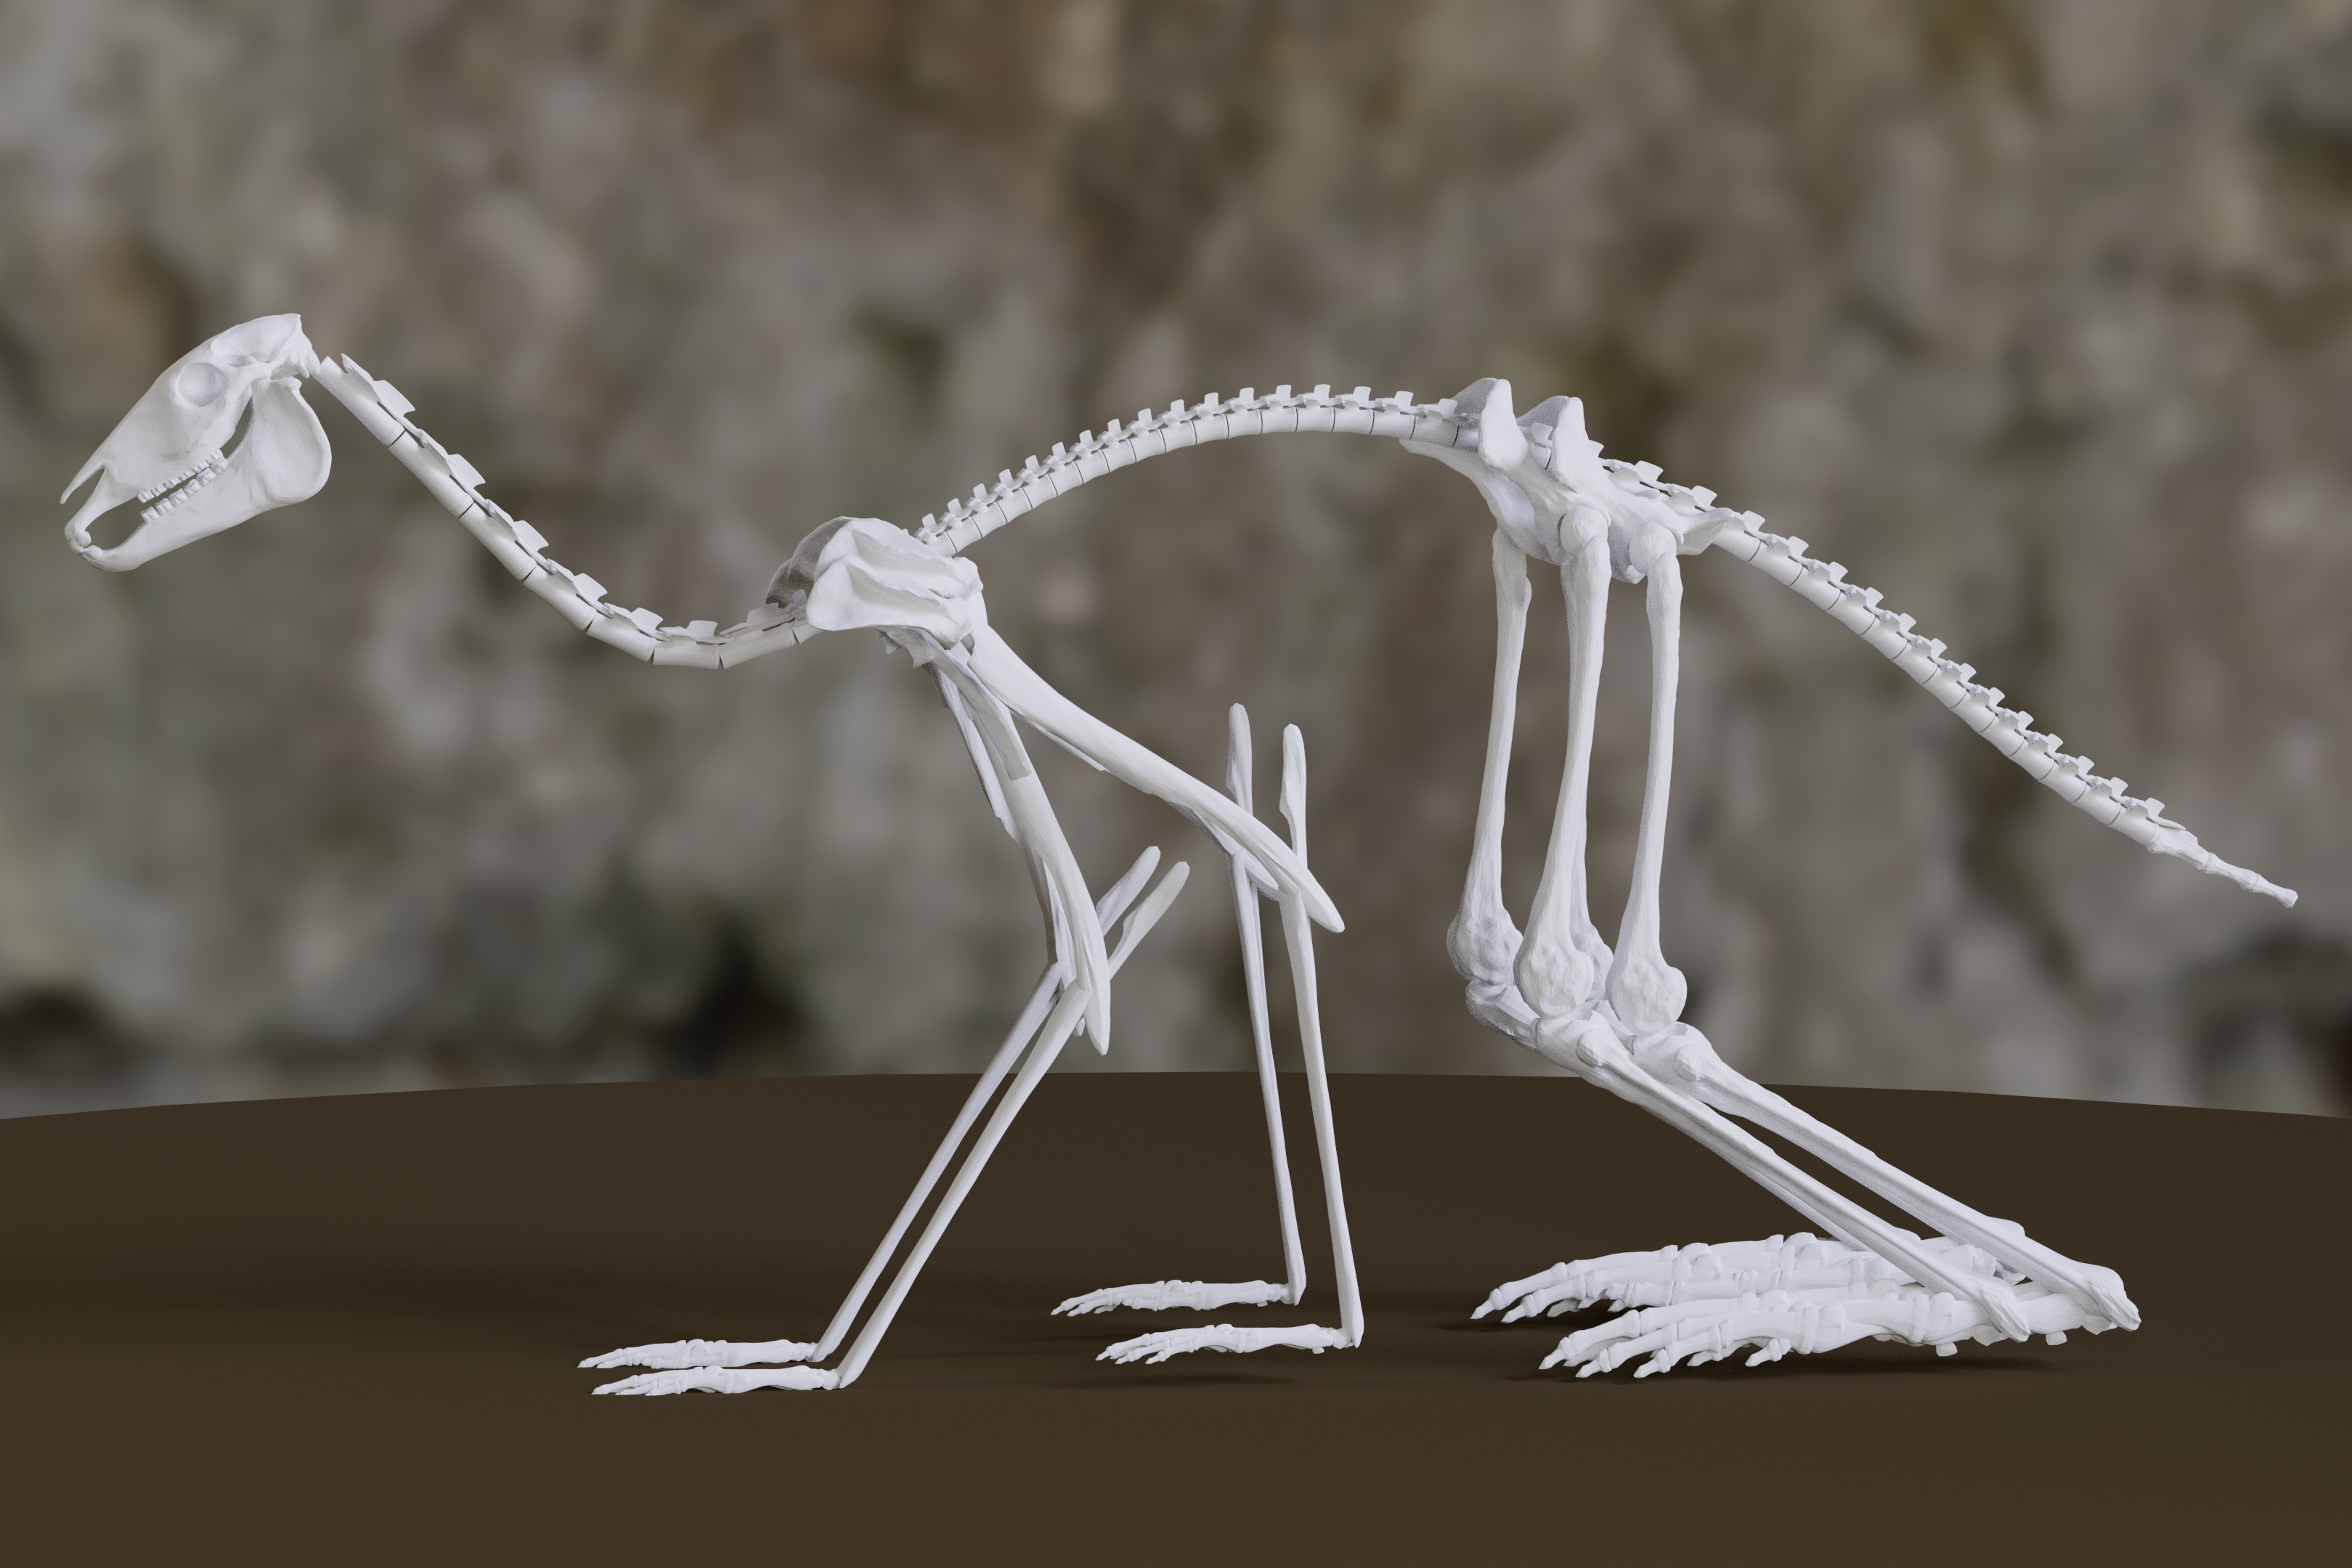
\includegraphics[height=5.8cm]{../java_skeleton_generation/example_skeletons/8legs.jpg}}~
 \subfloat[$1{,}5$ Flügel]{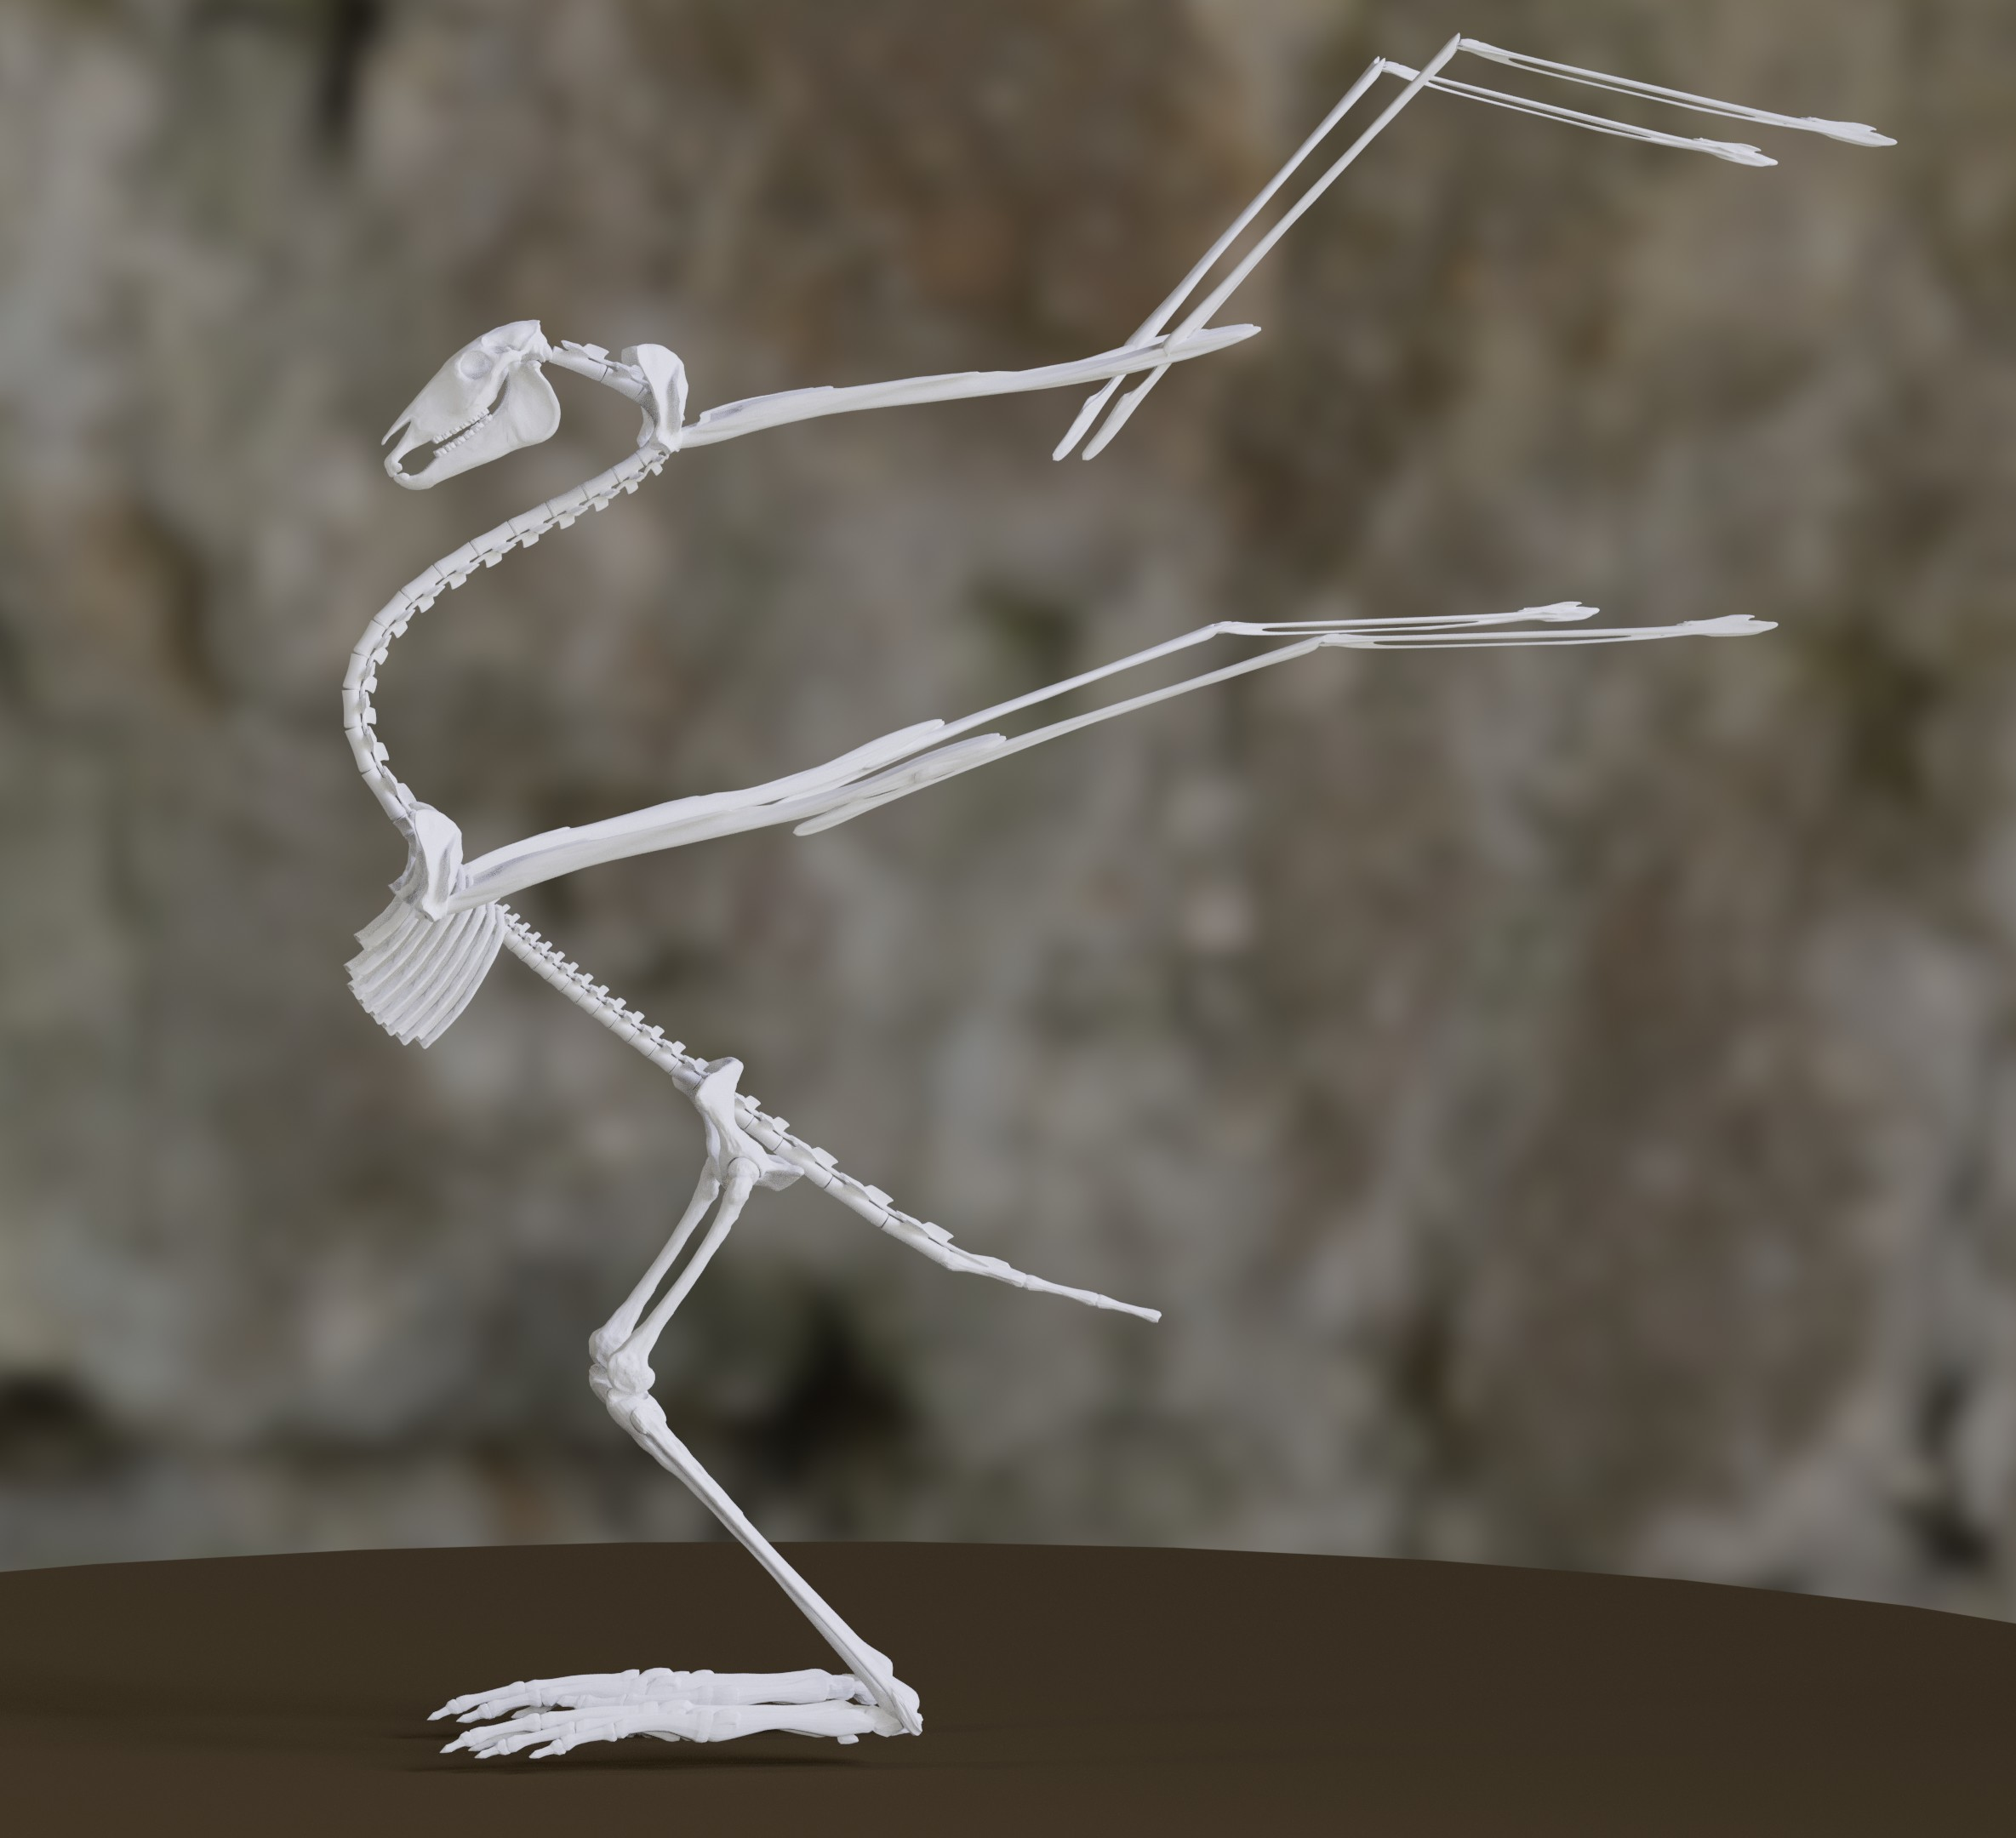
\includegraphics[height=5.8cm]{../java_skeleton_generation/example_skeletons/15wings.jpg}}
 
 \caption{Zwei Skelette, die mit extremen Bedingungen für die PCA generiert wurden. Als Hintergrund wurde \cite{background} verwendet. (a) Benutzereingabe: $8$ Beine und $4$ Beinpaare als Bedingung für \emph{Beine mit Bodenkontakt}. Es ist kein zweiter Schultergürtel am Hals erlaubt, aber zwei Extremitätenpaare pro Extremitätengürtel. (b) Benutzereingabe: $4$ Flügel und $1{,}5$ Flügelpaare als Bedingung für die PCA. Ein zweiter Schultergürtel am Hals wird erzwungen, aber es ist nur ein Extremitätenpaar pro Extremitätengürtel erlaubt.}
 \label{more_extremities}
\end{figure}

Die folgenden Eingaben werden durch die PCA berücksichtigt:
\begin{itemize}
 \item Die Anzahl der Beine mit Bodenkontakt (floored legs) muss eine gerade Zahl $n$ zwischen $0$ und $8$ sein. Als Bedingung für das Merkmal \emph{Paare von Beinen mit Bodenkontakt} wird dann $\frac{n}{2}$ verwendet. Bei echten Wirbeltieren liegt die Anzahl der Beine zwischen $0$ und $4$. Werden Werte größer $4$ als Bedingung an die PCA gestellt, so werden sehr stark geschwungene Wirbelsäulen generiert. Diese sehen aber, bis zu einem Wert von ca.\ $8$ gar nicht schlecht aus (siehe Abbildung \ref{more_extremities} a). Deshalb werden diese Werte auch als Bedingungen erlaubt. Sie werden nur mit einer gewissen Wahrscheinlichkeit etwas verkleinert, weil es auch möglich ist fantastische Tiere mit mehr als $4$ Beinen mit Wirbelsäulen für $4$-beinige Tiere zu generieren.
 
 \item Die Anzahl der Flügel (wings) muss ebenfalls gerade sein. Die Hälfte des Eingabewerts, aber maximal $1$, wird zu einer Bedingung für das Merkmal \emph{Flügel}.
 Die Wirbelsäulen, die unter Bedingungen für \emph{Flügel} größer $1$ generiert werden, sehen mit großer Wahrscheinlichkeit unrealistisch aus. Deshalb werden größere Werte nicht erlaubt. In Abbildung \ref{more_extremities} b ist ein Skelett zu sehen, dass einen Wert von $1{,}5$ für \emph{Flügel} hat. Dieser Wert kann tatsächlich noch erreicht werden, da ein zufälliger Wert aus $[-0{,}5, 0{,}5]$ auf die Bedingung aufaddiert wird. Bei noch größeren Werten ist der Hals noch extremer geschwungen.
 
 \item Die Zahlen für Arme (arms) und Flossen (fins) gehen nicht als Bedingung in die PCA ein (siehe Abschnitt \ref{section:extremity_generation}).
 
 \item Die $y$-Komponente des Abstands zwischen Kopf und Schultergürtel (neck $y$ length) und die $x$-Komponente des Abstands zwischen Hüfte und Schwanzspitze (tail $x$ length) können wiederum direkt als Bedingung an die PCA weitergegeben werden.
\end{itemize}

Die Anzahlen der verschiedenen Extremitätentypen werden außerdem verwendet, um die Parameter $e_v, e_h$ und $e_{v2}$ für die Anzahl der Vorder- und Hinterextremitäten der Grammatik (siehe Abschnitte \ref{section:grammar} und \ref{additional_extremities}) zu bestimmen und um den Typ und damit die Positionierung der verschiedenen generierten Extremitäten festzulegen (siehe Anfang Abschnitt \ref{section:extremity_generation}). Zusätzlich muss mit einberechnet werden, ob zwei Extremitätenpaare pro Extremitätengürtel erlaubt sind ($2$ extremities per girdle allowed?) und ob ein zweiter Schultergürtel auf dem Hals erlaubt, erzwungen oder verboten ist (second shoulder on neck?) (siehe auch Abschnitt \ref{additional_extremities}).

% Modell für Kopf
Außerdem gibt es theoretisch noch die Möglichkeit anzugeben, welches 3D-Modell für den Kopf verwendet werden soll (head kind). Leider gibt es hier, Stand Abschluss der Arbeit, nur eines zu Auswahl. Dies ließe sich aber leicht anpassen (siehe Abschnitt \ref{bone_models}).
Zusätzlich kann eingestellt werden, welche Auflösung das 3D-Modell haben soll (resolution). Hier gibt es die Möglichkeit nur Quader zu generieren oder Modelle von echten Knochen in niedriger oder hoher Auflösung einzusetzen.

% Dateiname, Anzahl und JavaView
Im Feld "`skeleton name"' kann der Dateiname des zu generierenden Modells eingestellt werden und in "`number of skeletons to generate"' kann festgelegt werden, wieviele Skelette auf einmal generiert werden sollen. Und schließlich kann man sich auch ein generiertes Modell anzeigen lassen (show skeleton). Dazu wird das Programm \emph{JavaView} \cite{JavaView} verwendet. Es ist darauf spezialisiert 3D-Geometrie interaktiv zu visualisieren und kann in Javacode eingebunden werden.


%------------------------------------------
\section{Speichern und Laden von Skeletten}
\label{load_skeletons}

Um ein vorgegebenes Skelett reproduzieren zu können, reicht es einige Metadaten zu speichern. Dazu gehören die Dimensionen der PCA (Position der Wirbelsäule, Länge der Knochen in den Extremitäten und Gewicht) und Daten, die zusätzlich generiert werden (Anzahl und Art der Extremitäten an den jeweiligen Extremitätengürteln, die Winkel an den Gelenken der Extremitäten, Anzahl der Wirbel und Rippen und welches 3D-Modell für den Kopf verwendet werden soll).
Das alles ist in wenigen Java-Klassen gebündelt. Deshalb können die Daten über Java-Serialisierung \cite{JavaSerialization} leicht in eine Textdatei geschrieben werden. Diese Datei kann dann wieder eingelesen werden, um die Klassen wieder herzustellen.

% gui
Im Benutzerinterface (Abbildung \ref{gui_screenshot}) kann diese Funktion verwendet werden, indem "`save metadata to file"' ausgewählt und ein Dateiname eingegeben wird. Dann wird für jedes generierte Skelett eine Textdatei mit dem angegebenen Namen generiert, die die serialisierten Daten enthält.
Um ein Skelett aus solch einer Textdatei zu laden, muss die entsprechende Datei bei "`load from file"' ausgewählt werden. Dann werden die dazugehörigen Java-Klassen wieder hergestellt und das gleiche 3D-Modell noch einmal generiert.

% kein metadaten nach außen
Das funktioniert natürlich nur über das implementierte Programm, das genau die serialisierten Java-Klassen enthält und liefert keine Zusatzinformationen zu dem generierten Skelett an den Benutzer. Solche Zusatzinformationen könnten aber hilfreich für die Weiterverarbeitung des erzeugten Modells sein. In weiterführenden Arbeiten könnten sie zusätzlich generiert werden. Hilfreiche Informationen könnten dabei \zb die Knochenhierarchie oder die Winkeleinschränkungen an den Gelenken sein.

% pca Beispiele laden
Zusätzlich gibt es die Funktion konkrete PCA-Eingabebeispiele auszuwählen (construct from example). Damit wird ein Skelett mit den Daten generiert, die für dieses Beispiel erhoben wurden. Mit einem PCA-Punkt sind aber noch nicht alle Daten festgelegt, die ein Skelett bestimmen. Es ist nur festgelegt welcher PCA-Punkt in Schritt 2 des Algorithmus ausgewählt wird, nicht welche konkreten Parameter die Grammatik bekommt oder welche Typen von Extremitäten generiert werden (siehe Abschnitt \ref{section:overview}). Deshalb werden zusätzlich die Benutzereingaben, \zb für die Anzahl der Arme, berücksichtigt.


%----------------------------------
\section{Erzeugung von Variationen}

Sucht man Inspiration zu einem bestimmten Typ von Skelett oder Tier, so kann es hilfreich sein Variationen zu einem vorgegebenen Skelett generieren zu können. 
Vielleicht wurde ein interessantes Skelett generiert und man möchte dazu schnell viele ähnliche Skelette finden.
Dies ist mit dem hier vorgestellten Algorithmus relativ leicht möglich. In der Benutzer"-oberfläche muss "`create variations"' ausgewählt werden.

Ein möglicher Ansatz wäre zur Erzeugung von Variationen genetische Algorithmen (siehe Abschnitt \ref{genetic_algorithms}) zu verwenden. Die PCA gibt aber schon einen Raum vor, in dem relativ leicht zufällige Punkte erzeugt werden können. Das lässt sich zur Erzeugung von Variationen gut ausnutzen. Deshalb wurden hier keine genetischen Algorithmen verwendet. 

% was ist gegeben
Als Grundlage für Variationen kann ein gespeichertes Skelett oder ein Eingabebeispiel der PCA dienen (siehe Abschnitt \ref{load_skeletons}). Es ist also mindestens ein Punkt mit den erhobenen Merkmalen für die PCA gegeben. Bei einem gespeicherten Skelett ist zusätzlich noch gegeben wieviele Wirbel, Rippen und Extremitäten generiert werden und welche Art von Extremität an welchem Ansatzpunkt beginnt. Mit Ansatzpunkten sind hier die Elternknochen von Extremitäten, also Schulterblatt und Beckenknochen(2), gemeint.
Ist nur ein Eingabebeispiel der PCA gegeben, so fehlen diese Angaben. Es werden aber zusätzlich Benutzereingaben, \zb zur Anzahl verschiedener Extremitätentypen, berücksichtigt.

% pca punkt variieren
Für die Variationen wird zwischen Eingabemerkmalen für die PCA und unabhängig generierten Daten unterschieden. Um Variationen von einem Punkt $p = (x_1, x_2,\dots, x_n)$ im PCA-Raum zu generieren, wird für jede Dimension eine neue Zufallszahl erzeugt. Dies ergibt dann einen Punkt $p' = (x_1', x_2',\dots,x_n')$. Ein $x_i'$ wird mit einer Normalverteilung zum Erwartungswert $x_i$ erzeugt.
Der konkrete Wert für die Varianz wurde experimentell bestimmt. Er sollte nicht zu groß sein, damit die generierten Skelette sich ähneln, aber auch nicht zu klein, damit sie sich etwas unterscheiden. In der Implementierung wird
die Hälfte der Varianz verwendet, die die PCA für Dimension $i$ berechnet hat, also die Hälfte des Eigenwerts, der zur $i$-ten Dimension gehört. 

% Rest variieren
Bei den Merkmalen, die unabhängig von der PCA sind, wird unterschiedlich vorgegangen. Wieviele Wirbel und Rippen generiert werden sollen wird einfach neu zufällig bestimmt. Dies ist also unabhängig vom gegebenen Skelett.\\
Für Typ und Anzahl der Extremitäten wird etwas mehr Aufwand betrieben, da dies mehr Einfluss auf das Aussehen des Skeletts hat.
Sind noch keine Ansatzpunkte und Typen von Extremitäten vorgegeben, werden diese zunächst berechnet. Dies passiert, wenn kein gespeichertes Skelett geladen, sondern ein PCA-Beispiel verwendet wird.
Danach wird ein Ansatzpunkt ausgelost. Wurde diesem Ansatzpunkt noch keine Extremität zugeteilt oder ist noch Platz für eine weitere, wird mit Wahrscheinlichkeit $0{,}5$ eine Extremität mit einem Typ, der an diesen Ansatzpunkt passt, hinzugefügt. Gibt es an dem Punkt hingegen schon eine Extremität, so wird ihr Typ, ebenfalls mit Wahrscheinlichkeit $0{,}5$, verändert. Wurde eine Veränderung ausgelost, wird die Extremität an dem gewählten Ansatzpunkt gelöscht und mit einer gewissen Wahrscheinlichkeit\footnote{Im Code wurde hier eine Wahrscheinlichkeit von $0{,}2$ verwendet.} wird eine Extremität mit gleichem Typ an einem anderen Ansatzpunkt wieder eingefügt, falls möglich.\\
Diese Prozedur verschiebt keine Knochen. Sie wird vor Ausführung der Grammatik durchgeführt. Das bedeutet, es wird bestimmt an welchen Stellen wieviele Vorder- und Hinterextremitäten generiert werden (Parameter $e_h, e_{h2}, e_s, e_{s2}, e_b$ und $e_{b2}$) und welchen Typ sie haben, also ob sie bei der Positionierung als Beine, Flügel, Flossen oder Arme behandelt werden.
Die Längen der Extremitäten werden durch $p'$ vorgegeben und hängen nur davon ab, ob es sich um Vorder- oder Hinterextremitäten handelt.

Sind alle Parameter für die Grammatik und die Typen der Extremitäten festgelegt, werden die Skelettelemente durch die Grammatik neu generiert. Dabei werden auch die Extremitäten neu positioniert.


%--------------------------------
%--------------------------------
\chapter{Implementierungsdetails}
\label{chapter:implementation_detail}

%---------------------------
\section{Programmiersprache}

\begin{itemize}
 \item Rust: nicht geeignet, da Datenstrukturen die zyklische Referenzen auf veränderbare Objekte verwenden nicht oder nur kompliziert umsetzbar sind.
 \item Java: scheint gut zu funktionieren. Es gibt Bibliotheken zum im-/exportieren von obj-Dateien und Unterstützung für OpenGL\\
 Außerdem gibt es Bibliotheken, die PCA (\bzw Kovarianzmatrizen \etc) unterstützen und JavaView um objs darzustellen
\end{itemize}


%---------------------
\section{Dateiformate}

\begin{itemize}
 \item Einfachstes Format (nur für die Darstellung von 3D-Objekten ohne Zusatzinformationen): obj
 \item Erster Schritt: einfaches .obj erzeugen und mit Blender darstellen; einfach Knochen als Bounding Box darstellen, später Verwendung von OpenGL mit vertex shadern \etc (Plan erwähnen? wurde ja doch nicht gemacht\dots)
 \item Jeder Editor geht mit Muskeln und Gelenken anders um. Gibt es ein Dateiformat, das nicht speziell zu einem Editor gehört, dass Bedingungen an die Rotation von Gelenken speichern kann?
 \item Eigenes Format erzeugen? Dann bräuchte man Plugins um es in verschiedenen Editoren laden zu können. Viel verwendeter Editor: Houdini (kostenlos für Studenten aber nicht Open Source). Oder selbst darstellen (siehe Interaktivität).
\item Vorschlag von Jo: "`Memory dumps"', also direkt die structs aus dem speicher auf platte rausschreiben. Am besten wenn sie am Stueck liegen mit einem fwrite() und zurücklesen mit einem fread(). Es ist nuetzlich dazu am Anfang der Datei ein bisschen Metadaten zu speichern (magic number, version, array size etc).
\end{itemize}

%- - - - - - - - - -
\subsection{OpenSim}

\begin{itemize}
 \item \url{https://simtk-confluence.stanford.edu:8443/display/OpenSim/OpenSim+Documentation}
 \item Open Source Software Platform für die Modellierung uns Simulation von Menschen, Tieren, etc.\\
 aber vor allem gedacht zur Auswertung von experimentellen Daten
 \item Import von .obj Dateien möglich. Außerdem zusätzliche Daten wie Winkel von Gelenken über .mot oder .sto Dateien (eigenes Format von OpenSim, siehe \url{https://simtk-confluence.stanford.edu:8443/display/OpenSim/Preparing+Your+Data})
 \item Export in andere Dateiformate nicht möglich (?)
 \item für Download und Zugang zur "`Community"' Account nötig
 \item für Windows und Mac OS (Linux Support gibt es auch, ist aber schwieriger: \url{https://simtk-confluence.stanford.edu:8443/display/OpenSim/Linux+Support})
\end{itemize}


%- - - - - - - -
\subsection{OBJ}

\begin{itemize}
 \item Beschreibung des Formats: \url{https://www.fileformat.info/format/wavefrontobj/egff.htm}
 \item Erzeugung mit Rust: obj\_exporter \url{https://docs.rs/obj-exporter/0.2.0/obj_exporter/index.html}
 \item Erzeugung mit Java: javagl Obj \url{https://github.com/javagl/Obj}, unterstützt auch Umwandlung von obj-Daten in Daten, die direkt für vertex buffer objects in OpenGL verwendet werden können
 \item Reicht wahrscheinlich für die ersten Dinge aus. Finetuning wird sowieso mit anderer Software gemacht
\end{itemize}

%- - - - - - - -
\subsection{FBX}

\begin{itemize}
 \item Verwendung am besten über Autodesk FBX SDK für C++. 
 \item Dokumentation: \url{http://help.autodesk.com/view/FBX/2019/ENU/} und \url{http://docs.autodesk.com/FBX/2014/ENU/FBX-SDK-Documentation/index.html}
 \item Es gibt auch fbxcel, eine FBX library für Rust. Ist aber relativ low level und nicht ganz offensichtlich wie zu verwenden.
 \item Einschränkungen für Gelenke können in FBX nicht gespeichert werden \url{http://docs.autodesk.com/FBX/2014/ENU/FBX-SDK-Documentation/index.html?url=cpp_ref/class_fbx_constraint.html,topicNumber=cpp_ref_class_fbx_constraint_htmlc57a3f99-513a-44a0-a24f-445e9077c99f}
\end{itemize}

%- - - - - - - - - -
\subsection{Alembic}

\begin{itemize}
 \item \url{www.alembic.io}
 \item Wird u.a. dafür verwendet Knochen (+ Animationen) in Ziva zu importieren
 \item Es kann mit Python (PyAlembic) und C++ verwendet werden.\\
 PyAlembic Doku: \url{http://docs.alembic.io/python/examples.html#pyalembic-intro}\\
 C++ API Refernce (enthält sehr wenig Infos): \url{http://docs.alembic.io/reference/index.html}
 \item Für Rust gibt es keine Bibliothek (?)
\end{itemize}


%----------------------------
\section{Aufbau der Software}

\begin{itemize}
 \item ein Wort zur Softwarearchitektur?
 \item Erweiterbarkeit der Software?
\end{itemize}


%-----------------------------
\section{Zufall}

Linearer Kongruenzgenerator reicht für Zufallszahlen aus, da nur wenige erzeugt werden (erkennbare Muster entstehen erst bei mehr Zufallszahlen) \todo{erwähnen?}


%--------------------------------
\section{Transformationsmatrizen}
\label{implementation_detail_matrices}

\todo{Recherchiere warum rechtshändige Koordinatensysteme bzw. konsistene Koordinatensysteme wichtig sind (back face culling, Rotationsrichtung der Matrizen bei positiven Winkeln)}

Jedes Element im Skelett speichert, relativ zu seinem Elternelement, die Position des Ursprungs seines Koordinatensystems. Um den Überblick über die Transformationsmatrizen bzw. Abbildungen behalten, die vom einen ins andere Koordinatensystem umwandeln, hier zwei Übersichtsgrafiken:
\todo{Erzeugung von Elementen auf der Wirbelsäule mit gegebener Weltposition + gespiegelte Elemente}

\begin{figure}
 \centering
 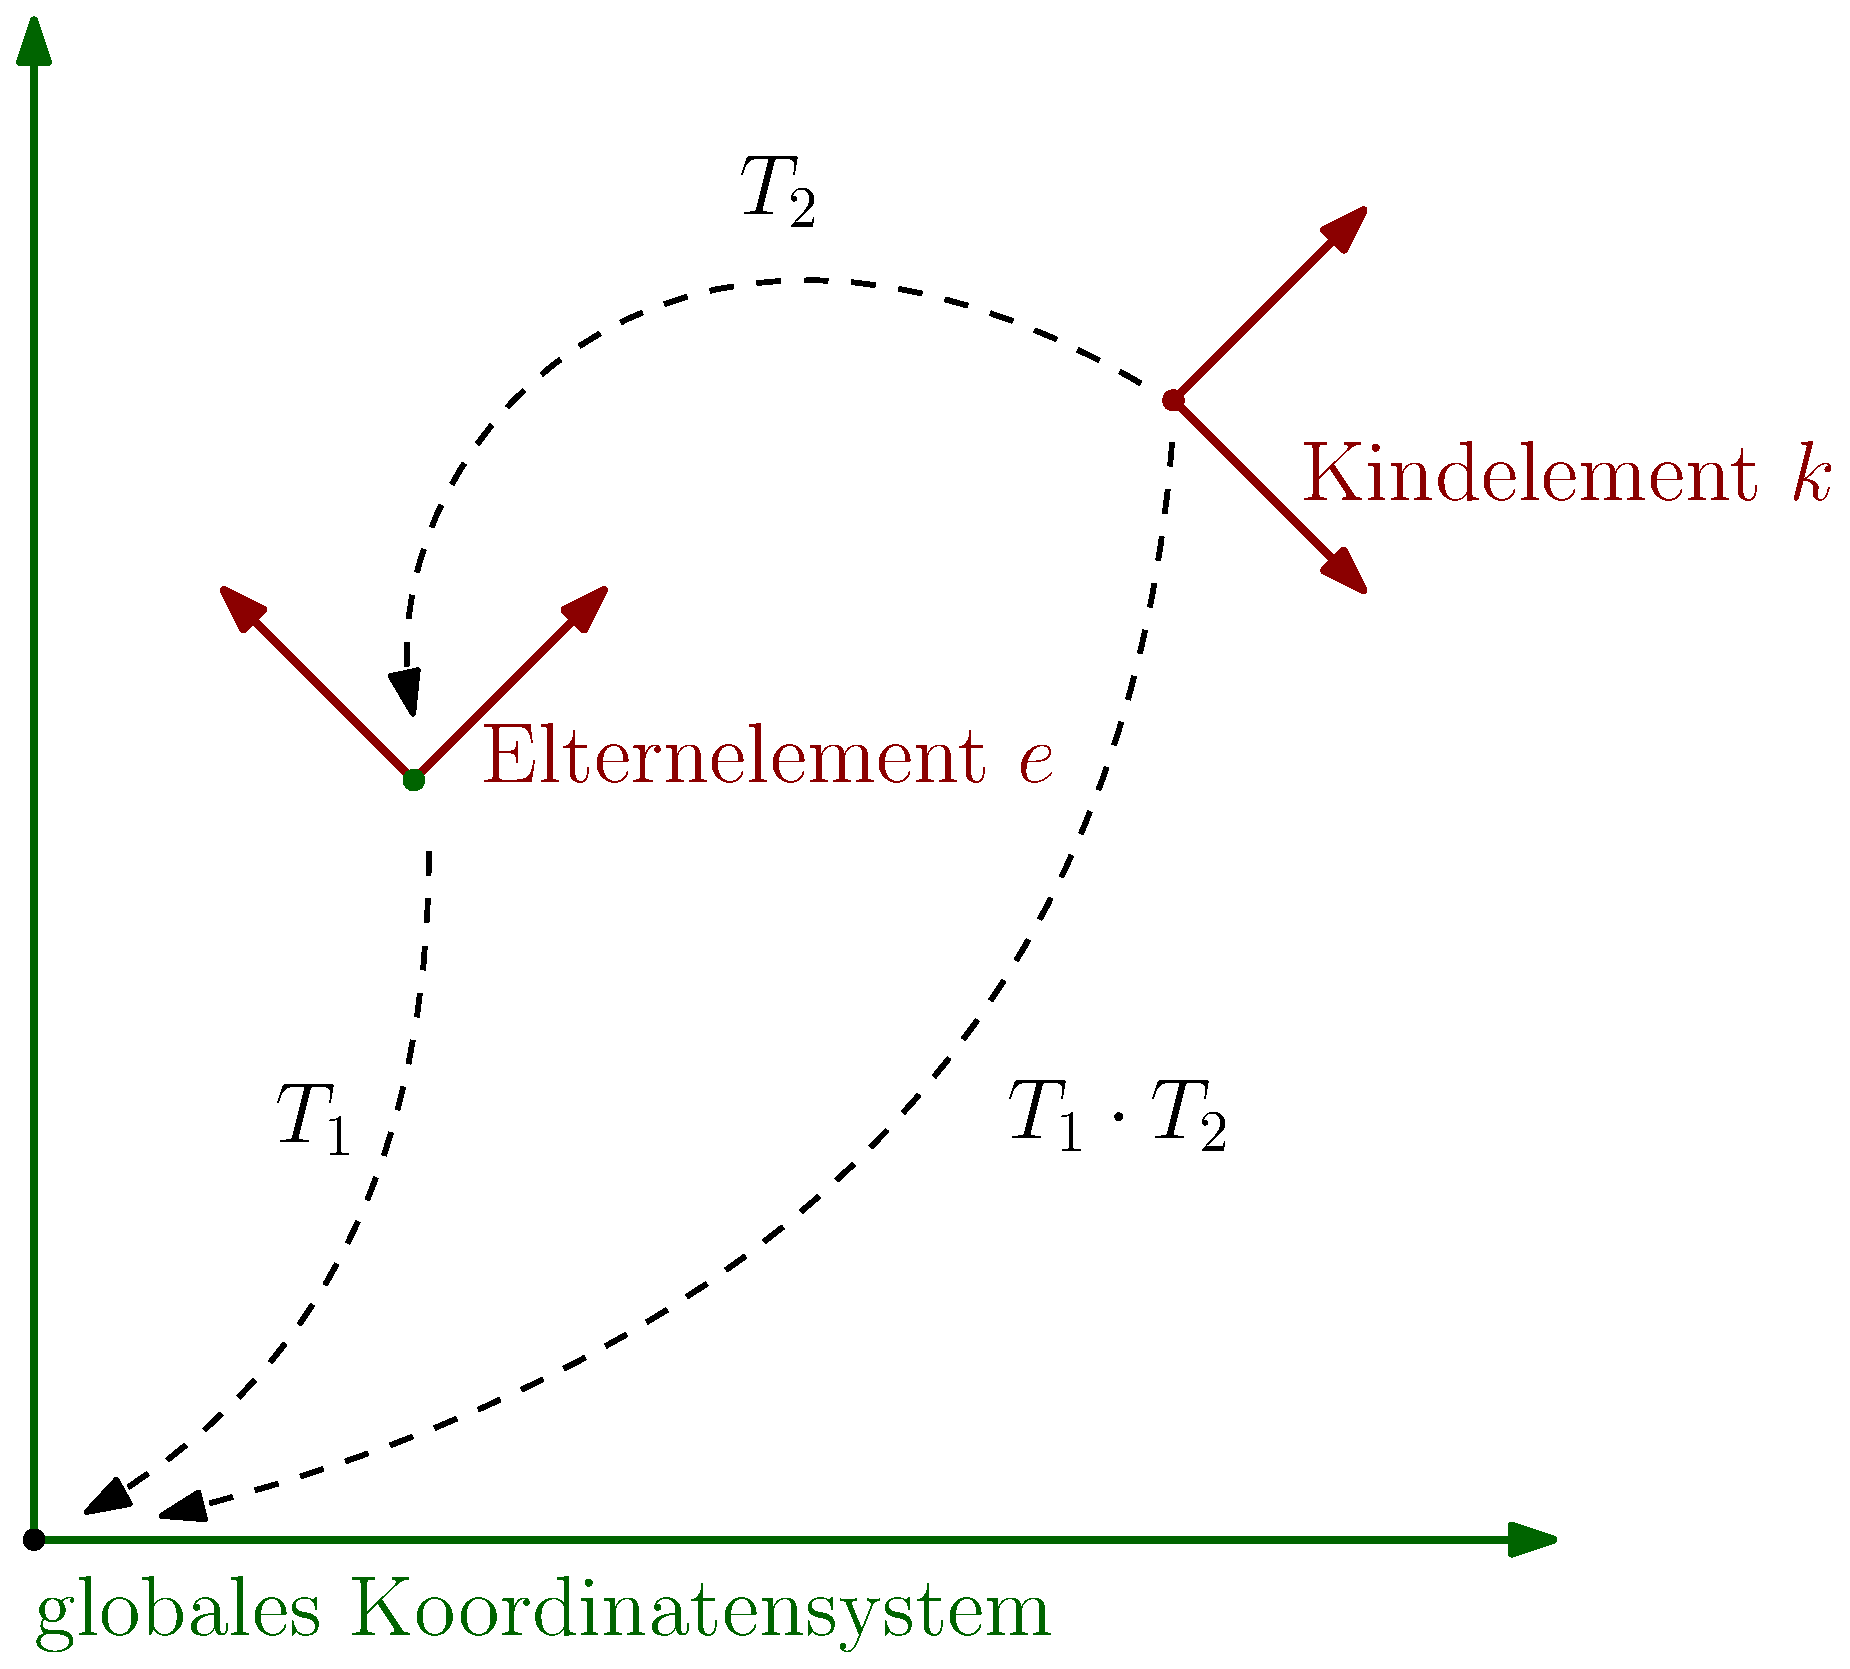
\includegraphics[width=0.6\textwidth]{graphics/transformation_matrices.eps}
 \caption{Gegeben sei das Element $e$. Die Abbildung, die die lokalen Koordinaten von $e$ in globale Koordinaten umrechnet sei $T_1$.
 Jedes Kindelement $k$ von $e$ speichert eine Transformationsmatrix $T_2$, die angibt wo der Ursprung des Koordinatensystems von $k$ relativ zum Koordinatensystem von $e$ liegt. Will mann nun Koordinaten von $k$ in globale Koordinaten umrechnen, benötigt man die Abbildung $T_1 \cdot T_2$.}
\end{figure}

\begin{figure}
 \centering
 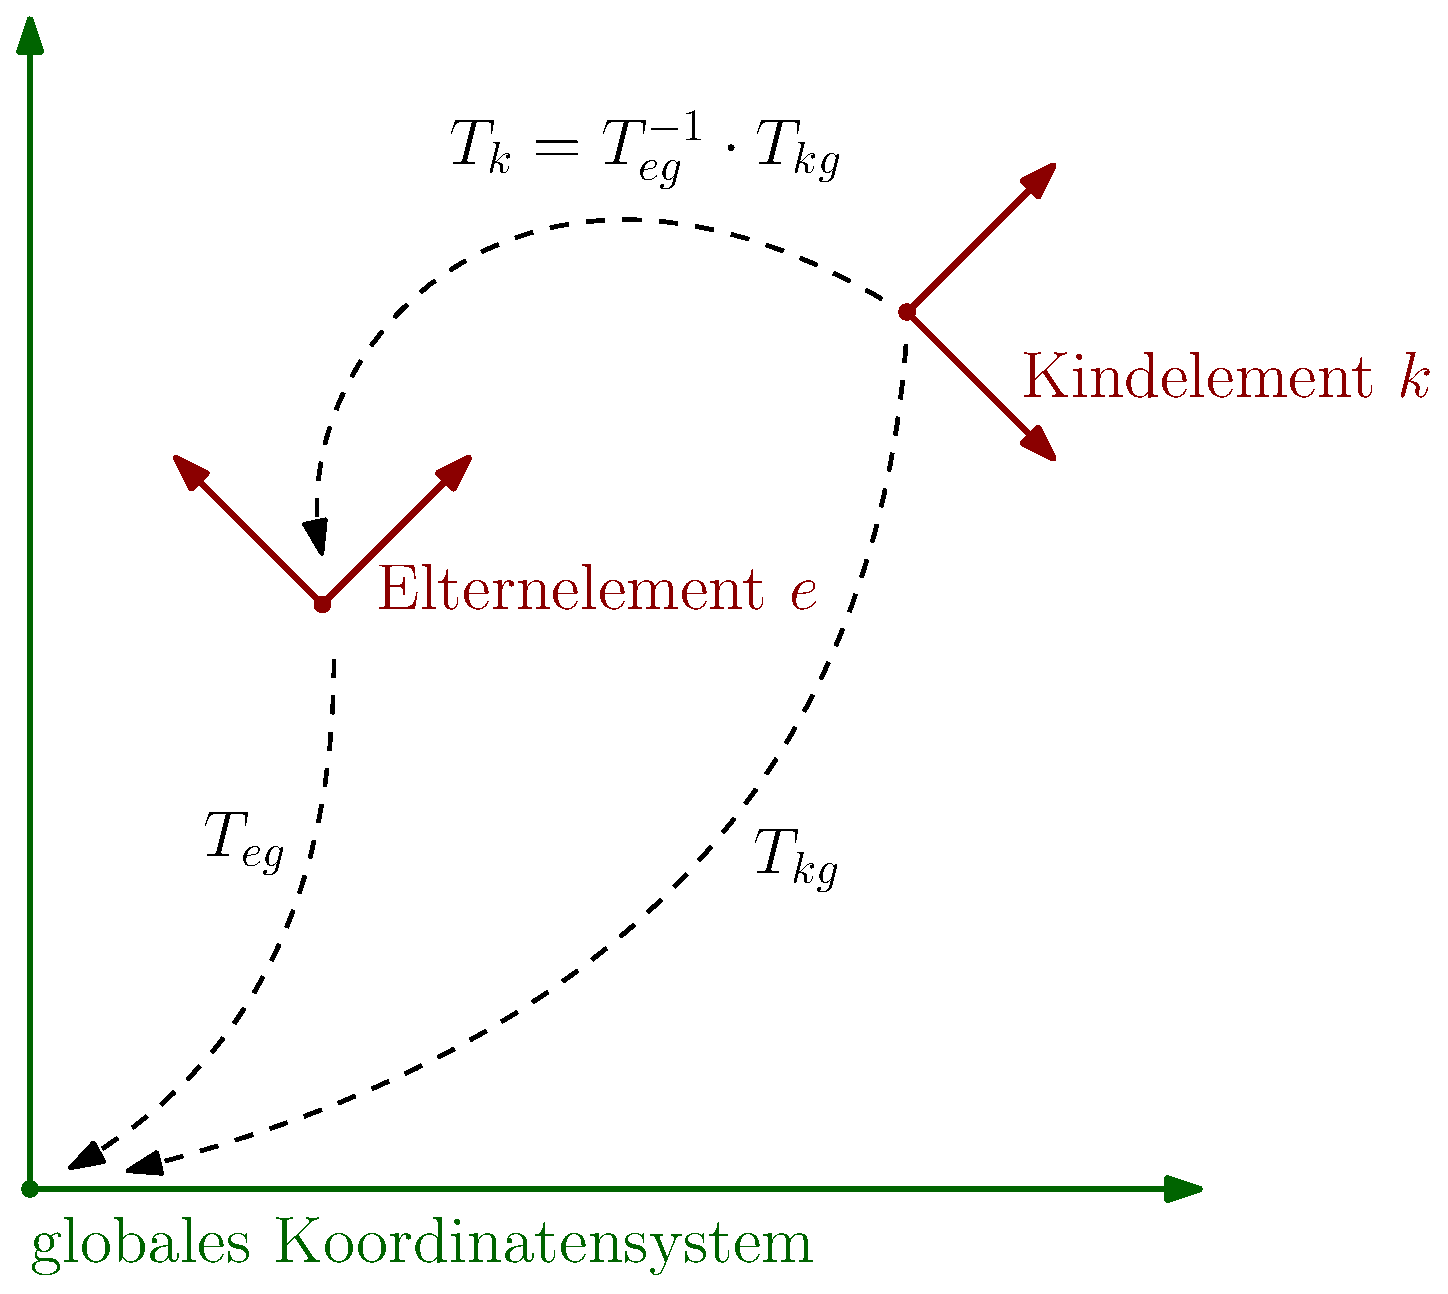
\includegraphics[width=0.6\textwidth]{graphics/transformation_matrices_spine.eps}
 \caption{Will man ein Element $k$ erzeugen, das Kindelement von $e$ ist und dessen globale Koordinaten bekannt sind, muss man die Abbildung berechnen, die die relative Position von $k$ angibt. Seien $T_1$ und $T_2$ jeweils die Transformationen in das globale Koordinatensystem von $e$ \bzw $k$. Dann ist die gesuchte Abbildung $T_1^{-1} \cdot T_2$.}
\end{figure}


%------------
\section{PCA}
\label{implementation_detail_pca}

Die Bilder der Skelette wurden folgendermaßen für die Datenerhebung vorbereitet:
 
 \begin{enumerate}
  \item Zuschneiden des Bildes, so dass möglichst nur das Skelett mit wenig Rand außen herum zu sehen ist.
  \item Einfügen in eine $1000 \times 1000$ Pixel große Bildumgebung.
  \item Verschieben innerhalb der Bildumgebung an den unteren Rand und horizontal in die Mitte.
 \end{enumerate}

 Ist das geschehen kann die Lage der Wirbelsäule und die Länge der Knochen der Extremitäten annotiert werden.
 
%- - - - - - - - - - - - - - - - -
\subsection{Annotation der Bilder}

Die Annotation der Bilder wurde per Hand mit dem Programm Inkscape\footnote{Programm zum erstellen und bearbeiten von Vektorgrafiken, \url{https://inkscape.org/de}} durchgeführt. Für jedes zu markierende Element wurde eine Strecke oder eine Bézierkurve eingefügt und mit einem vorher festgelegten Namen benannt. Diese Elemente wurden dann durch Inkscape als Pfade in der erzeugten svg-Datei gespeichert. Aus dieser Datei wurden dann automatisiert die eingetragenen Pfade mit ihren Koordinaten ausgelesen.

Folgende Details sind wichtig zu beachten, damit dieser Vorgang reibungslos abläuft. 
\begin{itemize}
 \item Man kann in Inkscape einstellen, dass Koordinaten immer absolut angegeben werden. Das ist sinnvoll um die Koordinaten leichter auslesen zu können.
 \item Der Ursprung des Koordinatensystems in Inkscape ist unten links, im svg-Format ist er aber oben links.
 \item Ebenen sollten in Inkscape nicht verschoben sein, sonst verschieben sich mit ihnen auch die Koordinaten.  
\end{itemize}

%- - - - - - - - - - - - - - - - - - - - - - - - - - - - - - - -
\subsection{Anpassung der PCA-Ergebnisse zur Weiterverarbeitung}

\begin{itemize}
 \item Um Wirbelsäule aus PCA Daten differenzierbar zu machen, wurden jeweils der vorletzte und der zweite Punkt von Hals und Rücken \bzw Rücken und Schwanz um den Kontaktpunk um den gleichen Winkel in gegensätzliche Richtungen gedreht, damit beide Bézierkurven an dem Kontaktpunkt die gleiche Steigung haben. \todo{beste Lösung?}
 \item An den Kontakpunkten der Wirbelsäulenteile ist die Steigung nicht unbedingt gleich (die Wirbelsäule als ganzes ist nicht $C^1$). Deshalb müssen vor der Weiterverwendung die jeweils nächsten Kontrollpunkte nach dem Kontakpunkt verschoben werden. Das wurde hier so gemacht, dass die zu verschiebenden Kontrollpunkte um den Kontakpunkt in gegensätzliche Richtungen rotiert wurden. Beide werden um den gleichen Winkel rotiert (siehe Abbildung \ref{smooth_spine}). Grundsätzlich könnten die Kontrollpunkte beliebig auf der Tangente des Kontaktpunkts platziert werden (rot im Bild) um eine übereinstimmende Steigung zu bekommen. Um den Verlauf der Wirbelsäulenteile möglichst wenig zu verändern ist es von Vorteil auch die Kontrollpunkte möglichst wenig zu verschieben. Man könnte die Punkte \zb auch senkrecht auf die Tangente projizieren. Welches Verfahren angewendet wird, ist jedoch nicht von großer Bedeutung. 
\end{itemize}

\begin{figure}
 \subfloat[vorher]{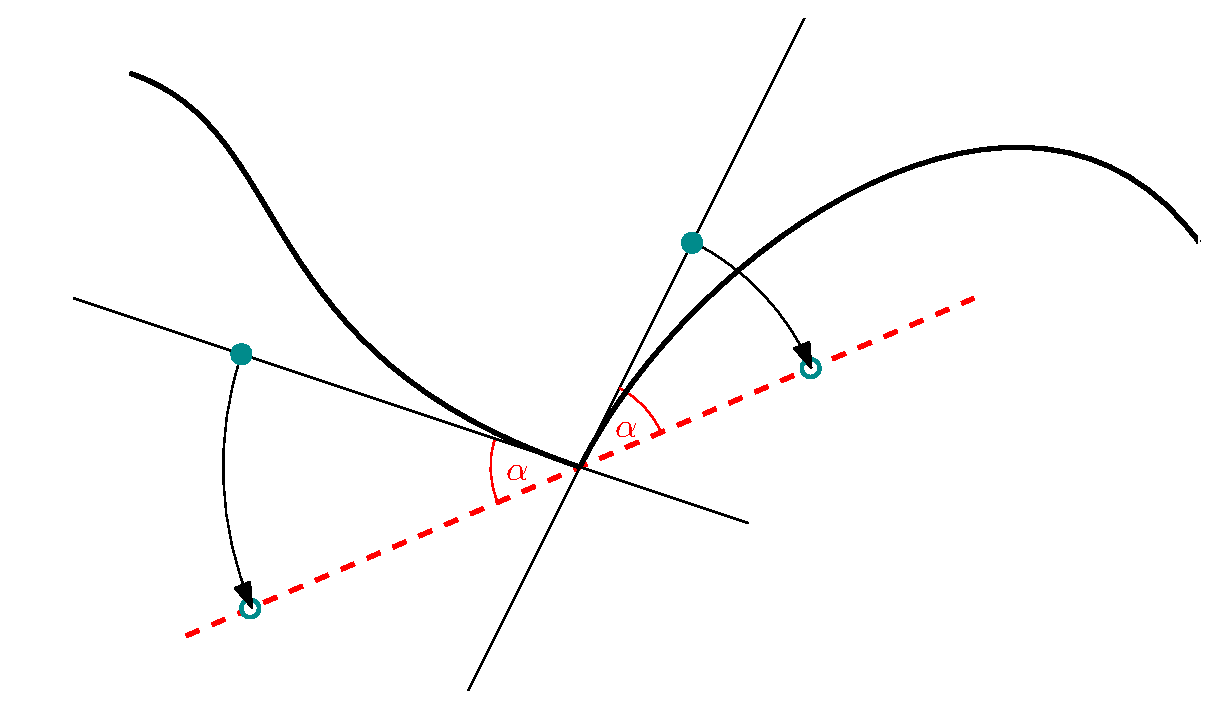
\includegraphics[width=0.5\textwidth]{graphics/smooth_spine1.eps}}
 \qquad
 \subfloat[nachher]{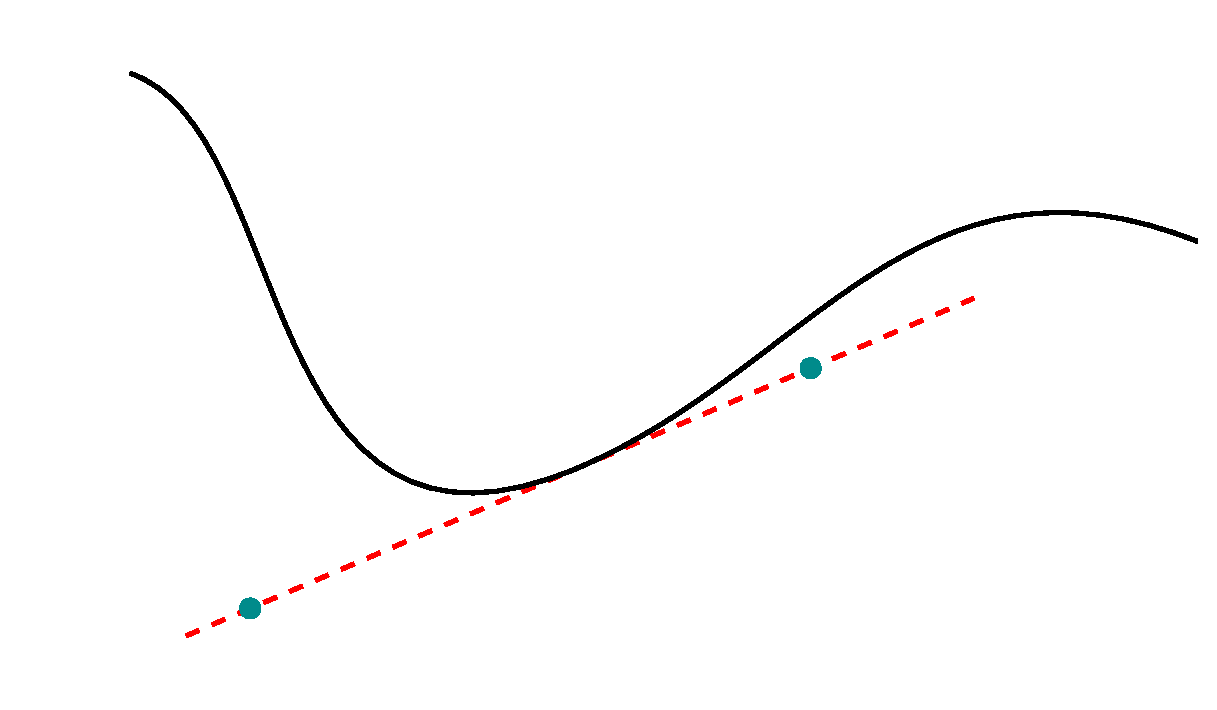
\includegraphics[width=0.5\textwidth]{graphics/smooth_spine2.eps}}
 \caption{Anpassung der Kontrollpunkte der Wirbelsäulenteile, wenn die Steigung an den Kontakpunkten ungleich ist. Die beiden Teile der Wirbelsäule und die Steigung am Kontaktpunkt sind hier in schwarz dargestellt. Die zu drehenden Kontollpunkte in cyan. In rot ist die resultierende Steigung und der Winkel, der für die Drehung verwendet wird, zu sehen.}
 \label{smooth_spine}
\end{figure}


%----------------
\section{Gelenke}

\todo{Für jede Art von Extremität und jede Position ein anderes Gelenk mit anderen Einschränkungen (nicht alle Möglichkeiten in einem)}

%----------------------------------------------------------
\section{Probleme der Beinpositionierung bei kurzen Beinen}
\label{leg_positioning_short_legs}

Wie in Absatz \ref{leg_algo} zur Ausrichtung der Beine bereits beschrieben, treten bei sehr kurzen Beinen ein paar Probleme auf. Diese werden im Folgenden kurz umrissen.

\begin{enumerate}
 \item % Bodenhöhe nicht von Gelenk aus gemessen
   Bei Berechnung der Bodenhöhe wird die Beinlänge von den entsprechenden Kontrollpunkten der Bézierkurve aus gemessen, da die Position der Hüfte/Schulter in diesem Stadium noch nicht klar ist. Deshalb kann es bei sehr kurzen Beinen sein, dass der Abstand zwischen Boden und Gelenk zu groß ist und der Boden nicht erreichbar ist.
   
   In diesem Fall wird das Bein einfach komplett ausgestreckt senkrecht nach unten positioniert. Da der Abstand zwischen dem Hüft- / Schultergelenk und dem Kontrollpunkt der Bézierkurve nicht sehr groß ist, ist auch der Abstand zu Bodenhöhe nicht enorm und fällt nicht allzusehr auf.
   
 \item % keine starke Änderung durch Drehung der Gelenke
   Bei sehr kurzen Knochen ändert sich der Abstand zum Boden durch Drehung der Gelenke nicht so stark wie bei langen Knochen. Wenn der Winkel sich zu wenig ändert, wird aber davon ausgegangen, dass die Winkeländerung zu klein ist und alle Änderungen sofort wieder zurückgesetzt wurden. Deshalb wird die Winkeländerung dann für die nächste Iteration stärker verkleinert. Das ist aber in diesem Fall kontraproduktiv. Der Algorithmus schafft es dann nämlich nicht mehr die Knochen in die richtige Lage zu bringen, da der Bewegungsspielraum dadurch zu stark eingeschänkt wird.
   
   Dem könnte man natürlich entgegenwirken, indem man, statt die Änderung des Abstandes zum Boden zu messen, abfragt wie oft die Drehungen in der jeweiligen Iteration zurückgesetzt wurden.
   
 \item % ganz kurze Beine
   Bei wirklich sehr kurzen Beinen (hier eine Gesamtlänge unter 5) macht es gar keinen Sinn sie anzuordnen, da man sie kaum sieht. Außerdem tritt hier der Effekt auf, der in Punkt 2 schon beschrieben wurde.
   
 \item % Beinstartpos unter Bodenhöhe
   Die Beinstartposition kann schon vor der ersten Iteration unterhalb der Bodenhöhe liegen. Das tritt auf, wenn mindestens ein Paar Beine sehr kurz ist und die Wirbelsäule an den Ansatzpunkten auf sehr unterschiedlicher Höhe liegt (siehe auch Absatz \ref{floor_height} zur Berechnung der Bodenhöhe).
   \todo{Beispiel: Dimetrodon}
   
   In diesem Fall ist der Algorithmus natürlich nicht anwendbar. Das Bein wird dann einfach senkrecht nach unten ausgerichtet und mit einem Fuß versehen, der mit der Sohle auf dem Boden steht.
   
 \item % Gelenkoffsets
   Bei kurzen Beinknochen kann es dazu kommen, dass der Oberschenkel nicht näher zum Boden kann, weil er schon aufliegt, aber Schienbein und Hand durch das Gelenkoffset (siehe Kapitel \ref{chapter:bone_models} zur Positionierung der Knochenmodelle) über dem Boden schweben und nicht näher zum Boden bewegt werden können.
   \todo{Beispiel Krokodil (siehe auch Screenshot)}
\end{enumerate}








%---------------------------
%---------------------------
\chapter{Fazit und Ausblick}
\label{chapter:conclusion}

% 1. Zusammenfassung: Was wurde in dieser Arbeit gemacht? Was waren die Schlüsselergebnisse? Diesmal jedoch zusammengefasst nochmals für einen Leser, der die vorherigen Seiten mit allen Details bereits gelesen hat.
% 
% 2. Adressaten der Verbesserung: Wem nützen die Verbesserungen/Beiträge der Arbeit? Inwieweit wird die Software-Technik durch die Arbeit verbessert?
% 
% 3. Aufbauende/Zukünftige Arbeiten: Welche nächsten Schritte sind geplant (erst kurzfristige, dann längerfristige)? Welche möglichen Lösungsansätze für noch bestehende Probleme sind denkbar? Wie könnten Folgearbeiten aussehen?

Das Ergebnis dieser Arbeit ist ein Algorithmus, der 3D-Modelle von Wirbeltierskeletten generiert, und eine Implementierung desselben. Die Daten, auf deren Grundlage der Algorithmus arbeitet, sind annotierte 2D-Bilder von Wirbeltierskeletten, \zb aus Lehrbüchern der Zoologie. 
Mit Hilfe einer \emph{Principal Component Analysis} (PCA) erhält man die Möglichkeit zufällig normalverteilte Punkte zu erzeugen, die der gleichen Verteilung folgen wie die Beispieldaten.
Ein so erzeugter Punkt liefert alle benötigten Informationen um ein Skelett zu generieren.
Diese Technik liefert ohne weitere Einschränkungen viele unterschiedliche Skelette, die in den allermeisten Fällen auch realistisch wirken.\\
Nur die Positionierung der Beine liefert in vielen Fällen keine schönen Ergebnisse. Um das zu verbessern wären weitere Informationen, \zb aus den 2D-Bildern, notwendig. Trotzdem kann das generierte Skelett als erster Eindruck \bzw Inspiration für ein Modell dienen. Wenn das erzeugte Skelett die Grundlage für ein animiertes Wesen sein soll, muss die Positionierung der Knochen ohnehin situationsgerecht angepasst werden.

Außerdem können gezielt Skelette mit bestimmten Eigenschaften generiert werden, indem eine PCA auf bedingten Verteilungen ausgeführt wird oder Variationen zu schon generierten Skeletten erzeugt werden. Dies ist sehr hilfreich, wenn man schon eine Vorstellung davon hat, wie das zu generierende Skelett ungefähr aussehen soll.

Eine kontextfreie Grammatik legt fest, welche Knochen generiert werden und wie das Skelett aufgebaut ist.
Durch zusätzliche Bedingungen wird sie so eingeschränkt, dass sie immer genau ein Skelett generiert. Man könnte die Vorschriften, die in der Grammatik kodiert sind, also stattdessen auch als einfachen Algorithmus formulieren.
Die Darstellung als Grammatik sorgt jedoch dafür, dass die Ersetzungsregeln relativ übersichtlich und leicht erweiterbar sind. 

Zusätzlich zu "`realistischen"' Wirbeltierskeletten lassen sich mit dem Algorithmus auch fantastische Skelette generieren. Es können zusätzliche Extremitäten und ein zusätzlicher Schultergürtel erzeugt werden, ohne dass die Datengrundlage verändert werden muss. Es werden die gleichen Beispielbilder von echten Wirbeltierskeletten verwendet.
Deshalb unterscheiden sich die fantastischen Skelette nicht zu sehr von echten Wirbeltierskeletten.  


\newpage
\paragraph{Ausblick}
In zukünftigen Arbeiten könnte es sinnvoll sein die Datengrundlage, also die Auswahl an 2D-Skelettbildern, zu erweitern. Das Beispiel Mensch wurde \zb außen vor gelassen (siehe Abschnitt \ref{pose}). Es könnte also getestet werden wie gut Skelette mit sehr aufrechter Wirbelsäule generiert werden können.\\
Außerdem könnte das Merkmal \emph{Gewicht}, das hier zwar erhoben, aber nicht verwendet wurde, in die Generierung mit einfließen, \zb in die Dicke der Knochen. Dabei sollte aber beachtet werden, dass die Knochendicke der Tiere nicht proportional zu ihrem Gewicht ist (siehe Abschnitt \ref{bigAndSmall}).

Die Sammlung der verwendeten 3D-Modelle von Knochen lässt sich relativ leicht durch weitere \bzw alternative Modelle erweitern (siehe Abschnitt \ref{bone_models}). Um die Benutzung des Programms noch flexibler zu machen, könnte es so ergänzt werden, dass die zu verwendenden Knochenmodelle vom Benutzer selbst vorgegeben werden können.\\
Des Weiteren könnte der Algorithmus auch interaktiv gestaltet werden, um dem Benutzer noch mehr Kontrolle über die Generierung zu geben. Diese könnte \zb schrittweise erfolgen, mit der Möglichkeit nach jedem Schritt einzugreifen. Der Benutzer könnte dabei beispielsweise Schritte rückgängig machen, Skelettteile, die ihm nicht gefallen, neu generieren oder zusätzliche Bedingungen angeben.

Aufgrund der Zeitvorgabe beschränkt sich diese Arbeit auf die Generierung von Skeletten. Es werden weder Muskeln noch Haut generiert. Es wäre aber möglich den hier vorgestellten Algorithmus entsprechend zu erweitern. Dies würde einen noch plastischeren Eindruck der generierten Tiere liefern und die Modellierung von sehr wirklichkeitsnahen Wirbeltieren noch mehr vereinfachen.





%% --------------------
%% |   Bibliography   |
%% --------------------

%% Add entry to the table of contents for the bibliography
\printbibliography[heading=bibintoc]

%% ----------------
%% |   Appendix   |
%% ----------------
\begin{appendices}
%-------------------------------
%-------------------------------
\chapter{PCA Daten}
\label{appendix_pca}

%-----------------------------
\section{Eingabedaten für PCA}

%- - - - - - - - - 
\subsection{Bilder}
\label{picture_sources}
 
 Alle Bilder, die als Eingabe für die PCA verwendet wurden, sind in Abbildung \ref{all_images} zu finden. Im Folgenden sind die Bildquellen aufgezählt.
 Alle Tiere, die nicht aufgezählt sind, sind aus \cite{Spezielle_Zoologie} entnommen.
 \begin{itemize}
  \item Archaeopteryx, Ichthyosaurus, Ichthyostega, Urpferdchen aus \cite{Zoologie24Wehner}
  \item Blauwal \url{https://www.quagga-illustrations.de/wp-content/uploads/2014/05/h0001705.jpg}
  \item Chamäleon \url{https://www.madcham.de/de/anatomie/}
  \item Dormedar \url{https://upload.wikimedia.org/wikipedia/commons/a/ac/Camel_Skeleton_-_Richard_Owen_-_On_the_Anatomy_of_Vertebrates_\%281866\%29.jpg}
  \item Giraffe\\ \url{https://de.wikipedia.org/wiki/Giraffen#/media/Datei:Giraffe_skeleton.jpg}
  \item Gnu \url{https://lutzmoeller.net/Afrika/2007/Lutz-Juli/8-Gnu.php}
  \item Känguru \url{http://www.bildwoerterbuch.com/tierreich/beuteltiere/kaenguru/skelett-eines-kaengurus.php}
  \item Krokodil \url{https://de.depositphotos.com/210906852/stock-illustration-skeleton-crocodile-vintage-line-drawing.html}
  \item Pferd \url{https://www.kosmos.de/content/buecher/ratgeber/pferde-reiten/vorwaerts-abwaerts-eine-frage-der-haltung/}
  \item Schlange: zu Schlangen gibt es keine Bilder, die deren Skelett in ausgestrecktem Zustand von der Seite darstellen. Deshalb wurde ein leeres Bild genommen und der Verlauf des Rückens durch eine Gerade angenähert (Extremitäten besitzt eine Schlange nicht. Außerdem ist nicht erkennbar ob \bzw wo Hals in Rücken und Rücken in Schwanz übergeht. Deshalb wurde die komplette Wirbelsäule als Rücken markiert.)
  \item Schwan \url{https://www.alamy.de/skelett-eines-schwans-osteographia-oder-die-anatomie-der-knochen-london-1733-quelle-47-ich-12-kapitel-v-saitenhalter-autor-cheselden-william-image226921369.html}
  \item Sinornis und Taube aus \cite{Vergleichende_Anatomie}
  \item Strauß \url{https://www.alamy.de/stockfoto-skelett-von-strauss-24658845.html}
  \item Tyrannosaurus Rex \url{https://upload.wikimedia.org/wikipedia/commons/9/9f/Tyrannosaurus_skeleton.jpg}
 \end{itemize}
 
\begin{figure}
\subfloat[Afrikanischer Elefant]{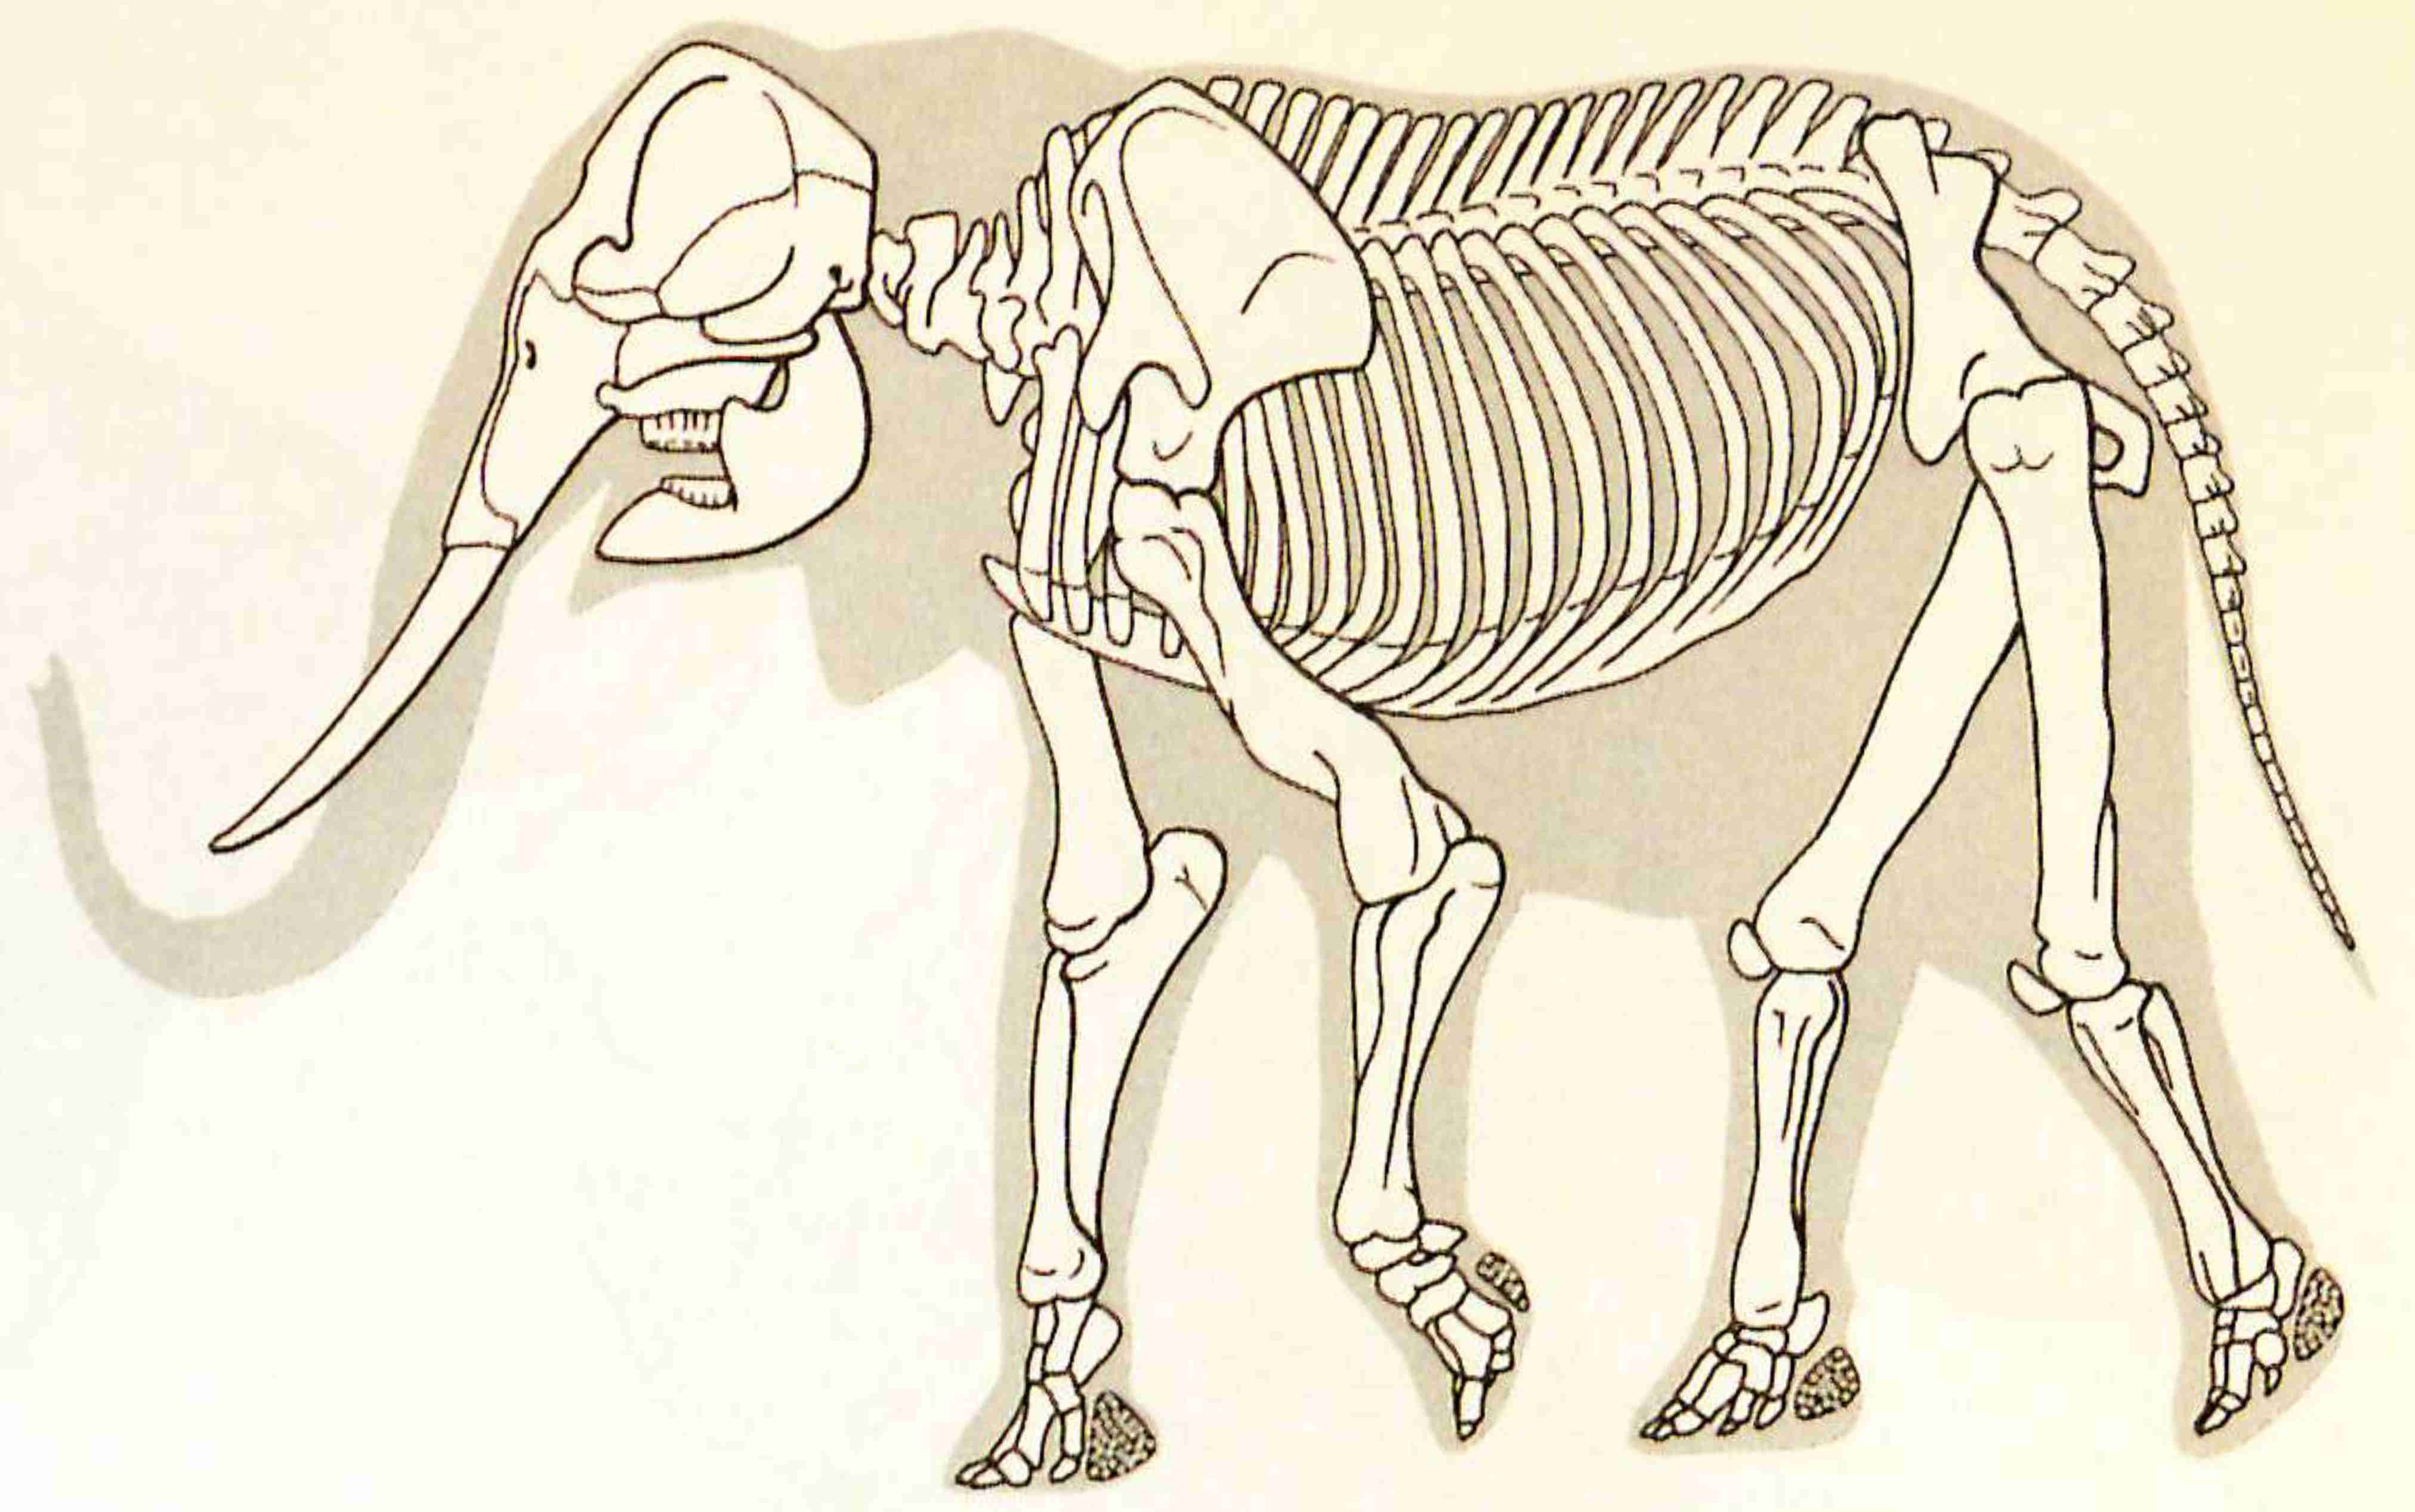
\includegraphics[width=0.2\textwidth]{../PCA/Skelettbilder_klein/Afrikanischer_Elefant.jpg}}~
\subfloat[Amerikanischer Flussbarsch]{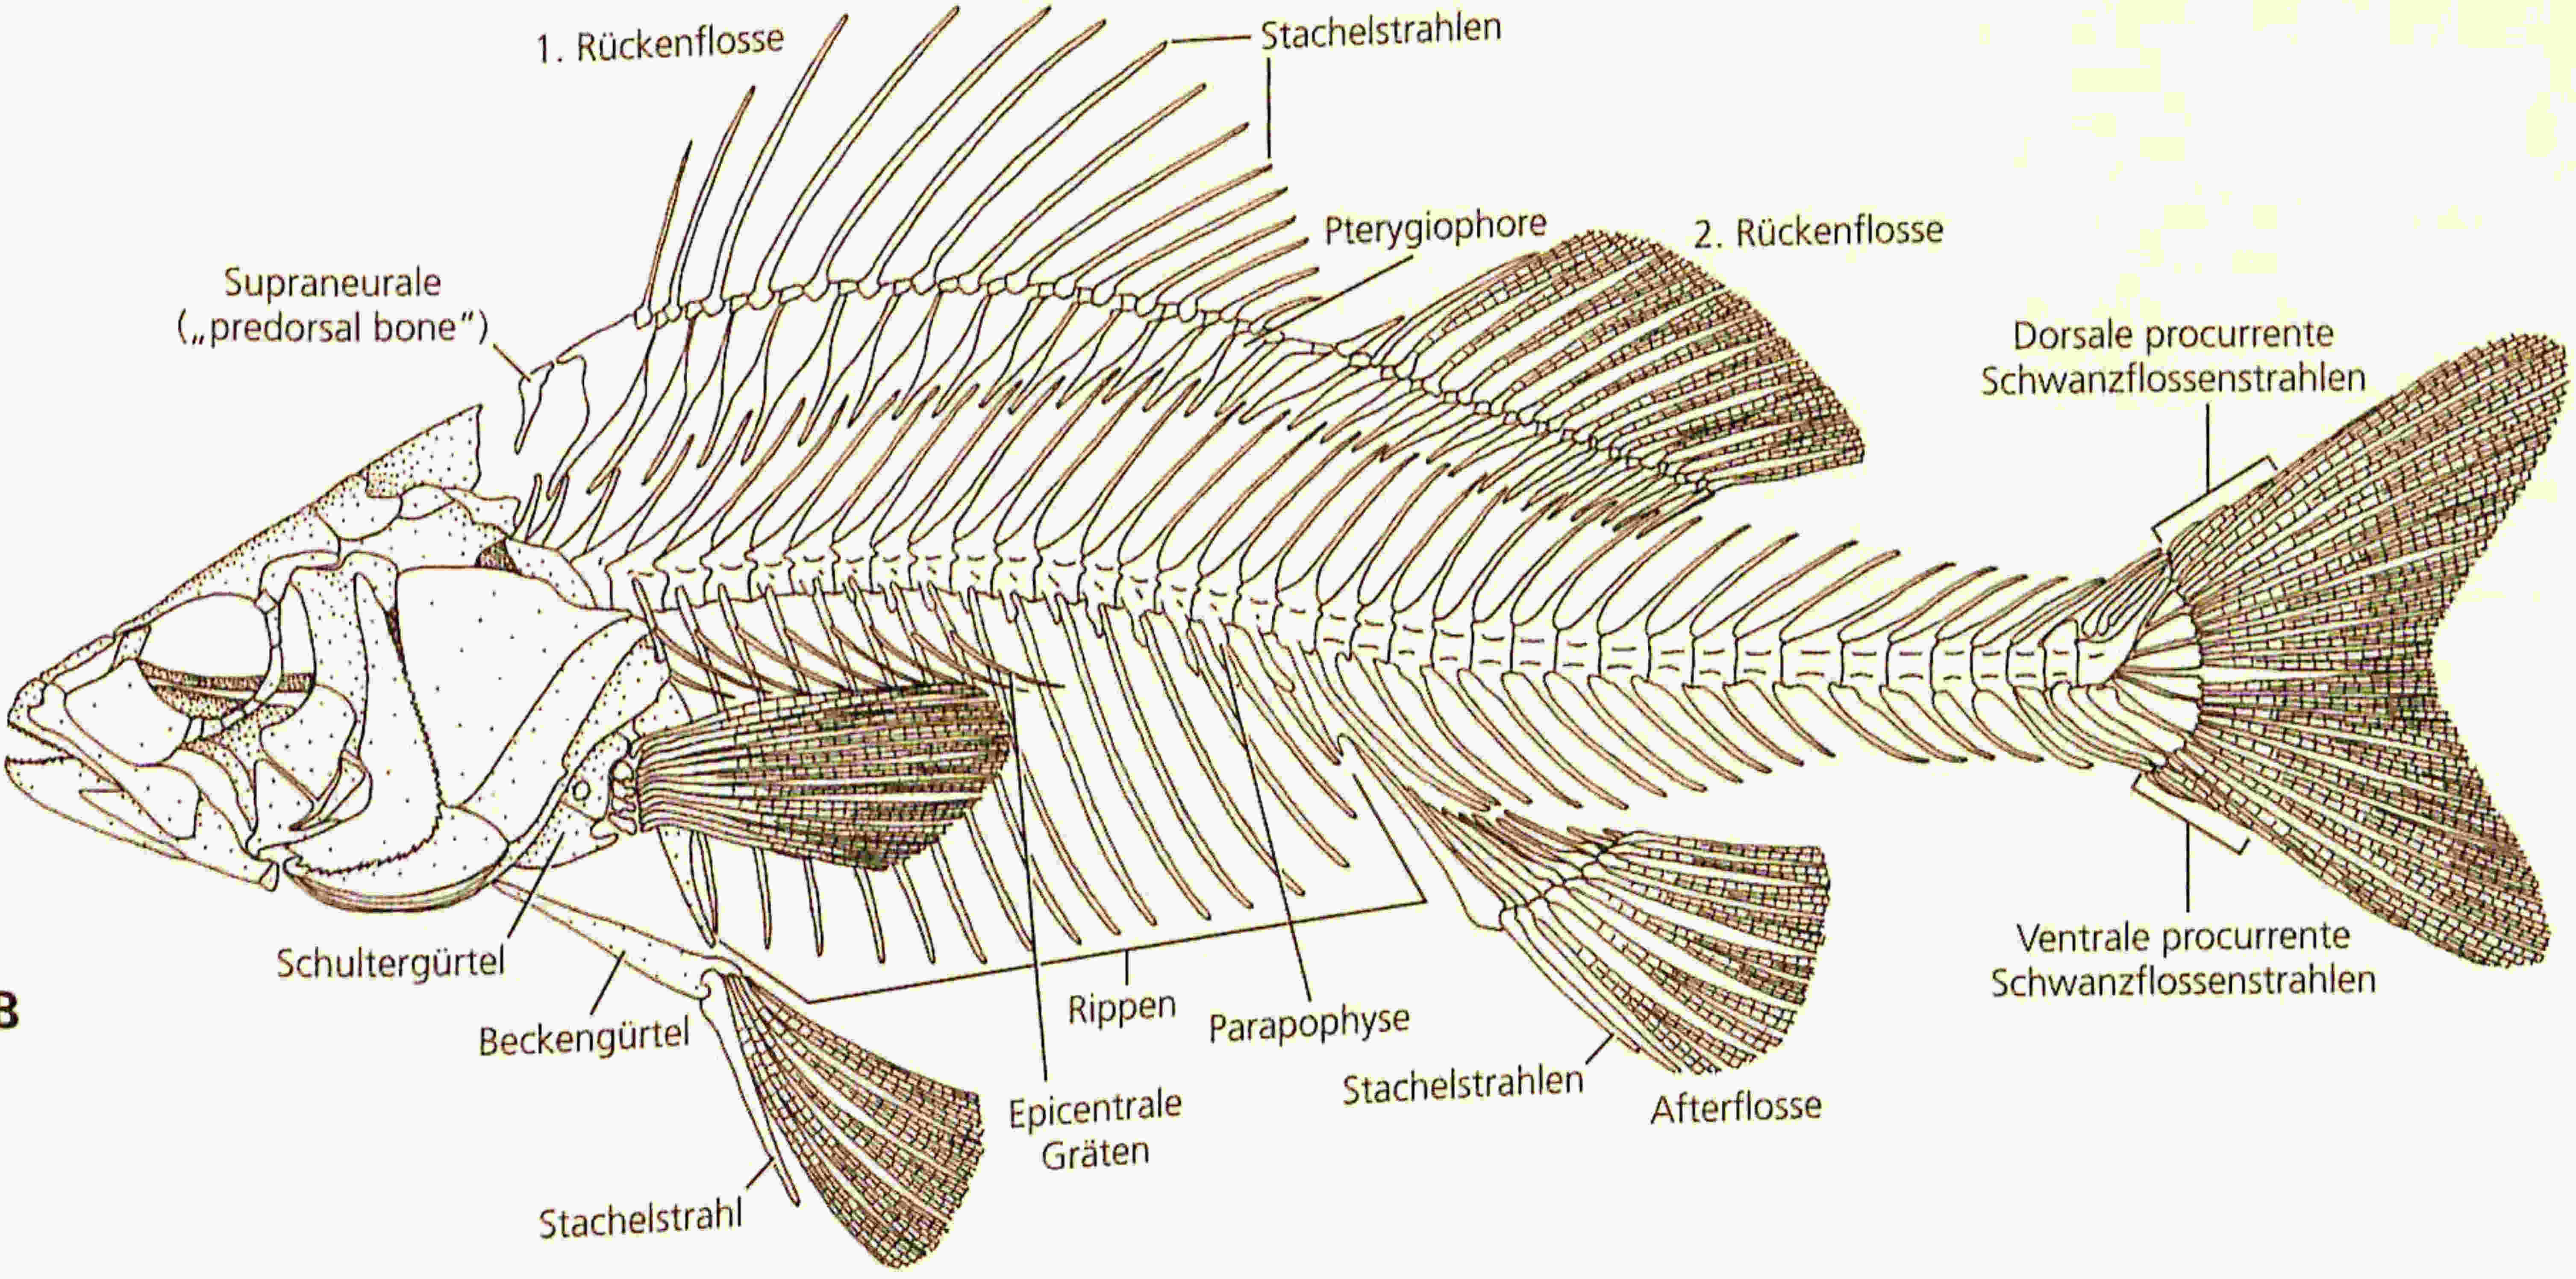
\includegraphics[width=0.2\textwidth]{../PCA/Skelettbilder_klein/Amerikanischer_Flussbarsch.jpg}}~
\subfloat[Archaeopteryx]{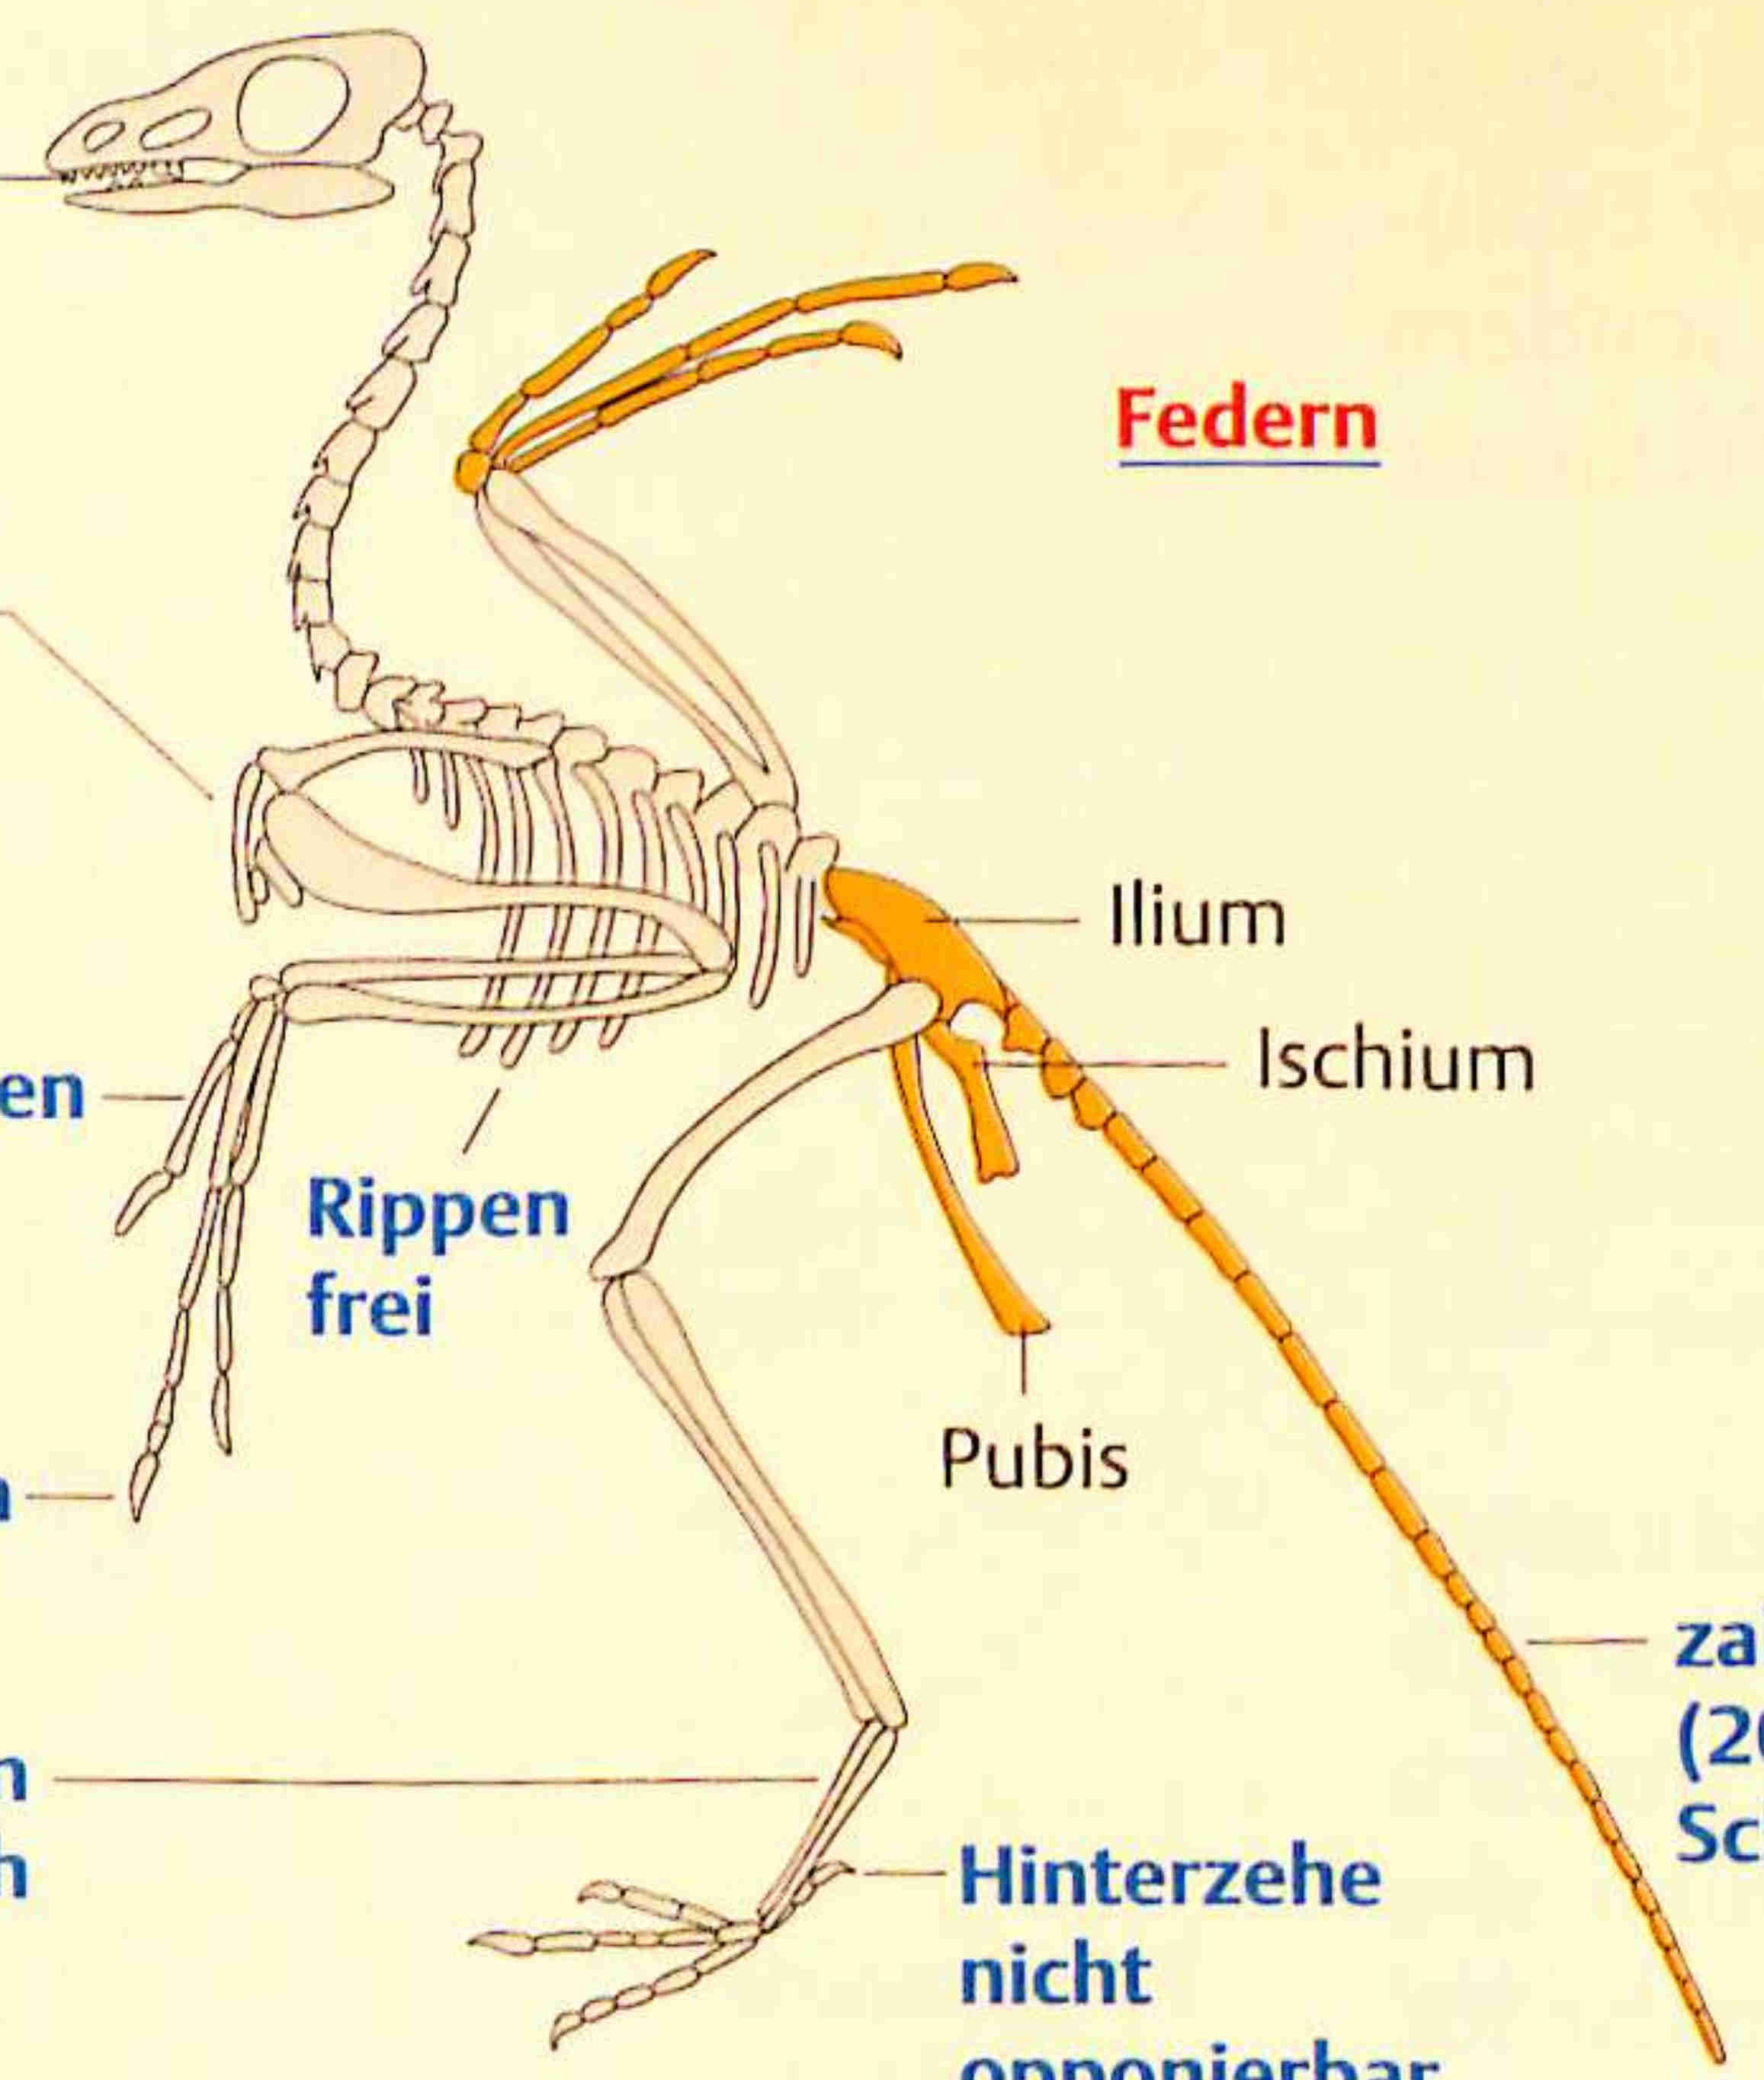
\includegraphics[width=0.2\textwidth]{../PCA/Skelettbilder_klein/Archaeopteryx.jpg}}~
\subfloat[Blauwal]{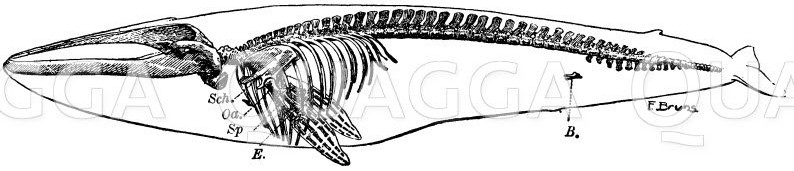
\includegraphics[width=0.2\textwidth]{../PCA/Skelettbilder_klein/Blauwal.jpg}}~
\subfloat[Brachiosaurus]{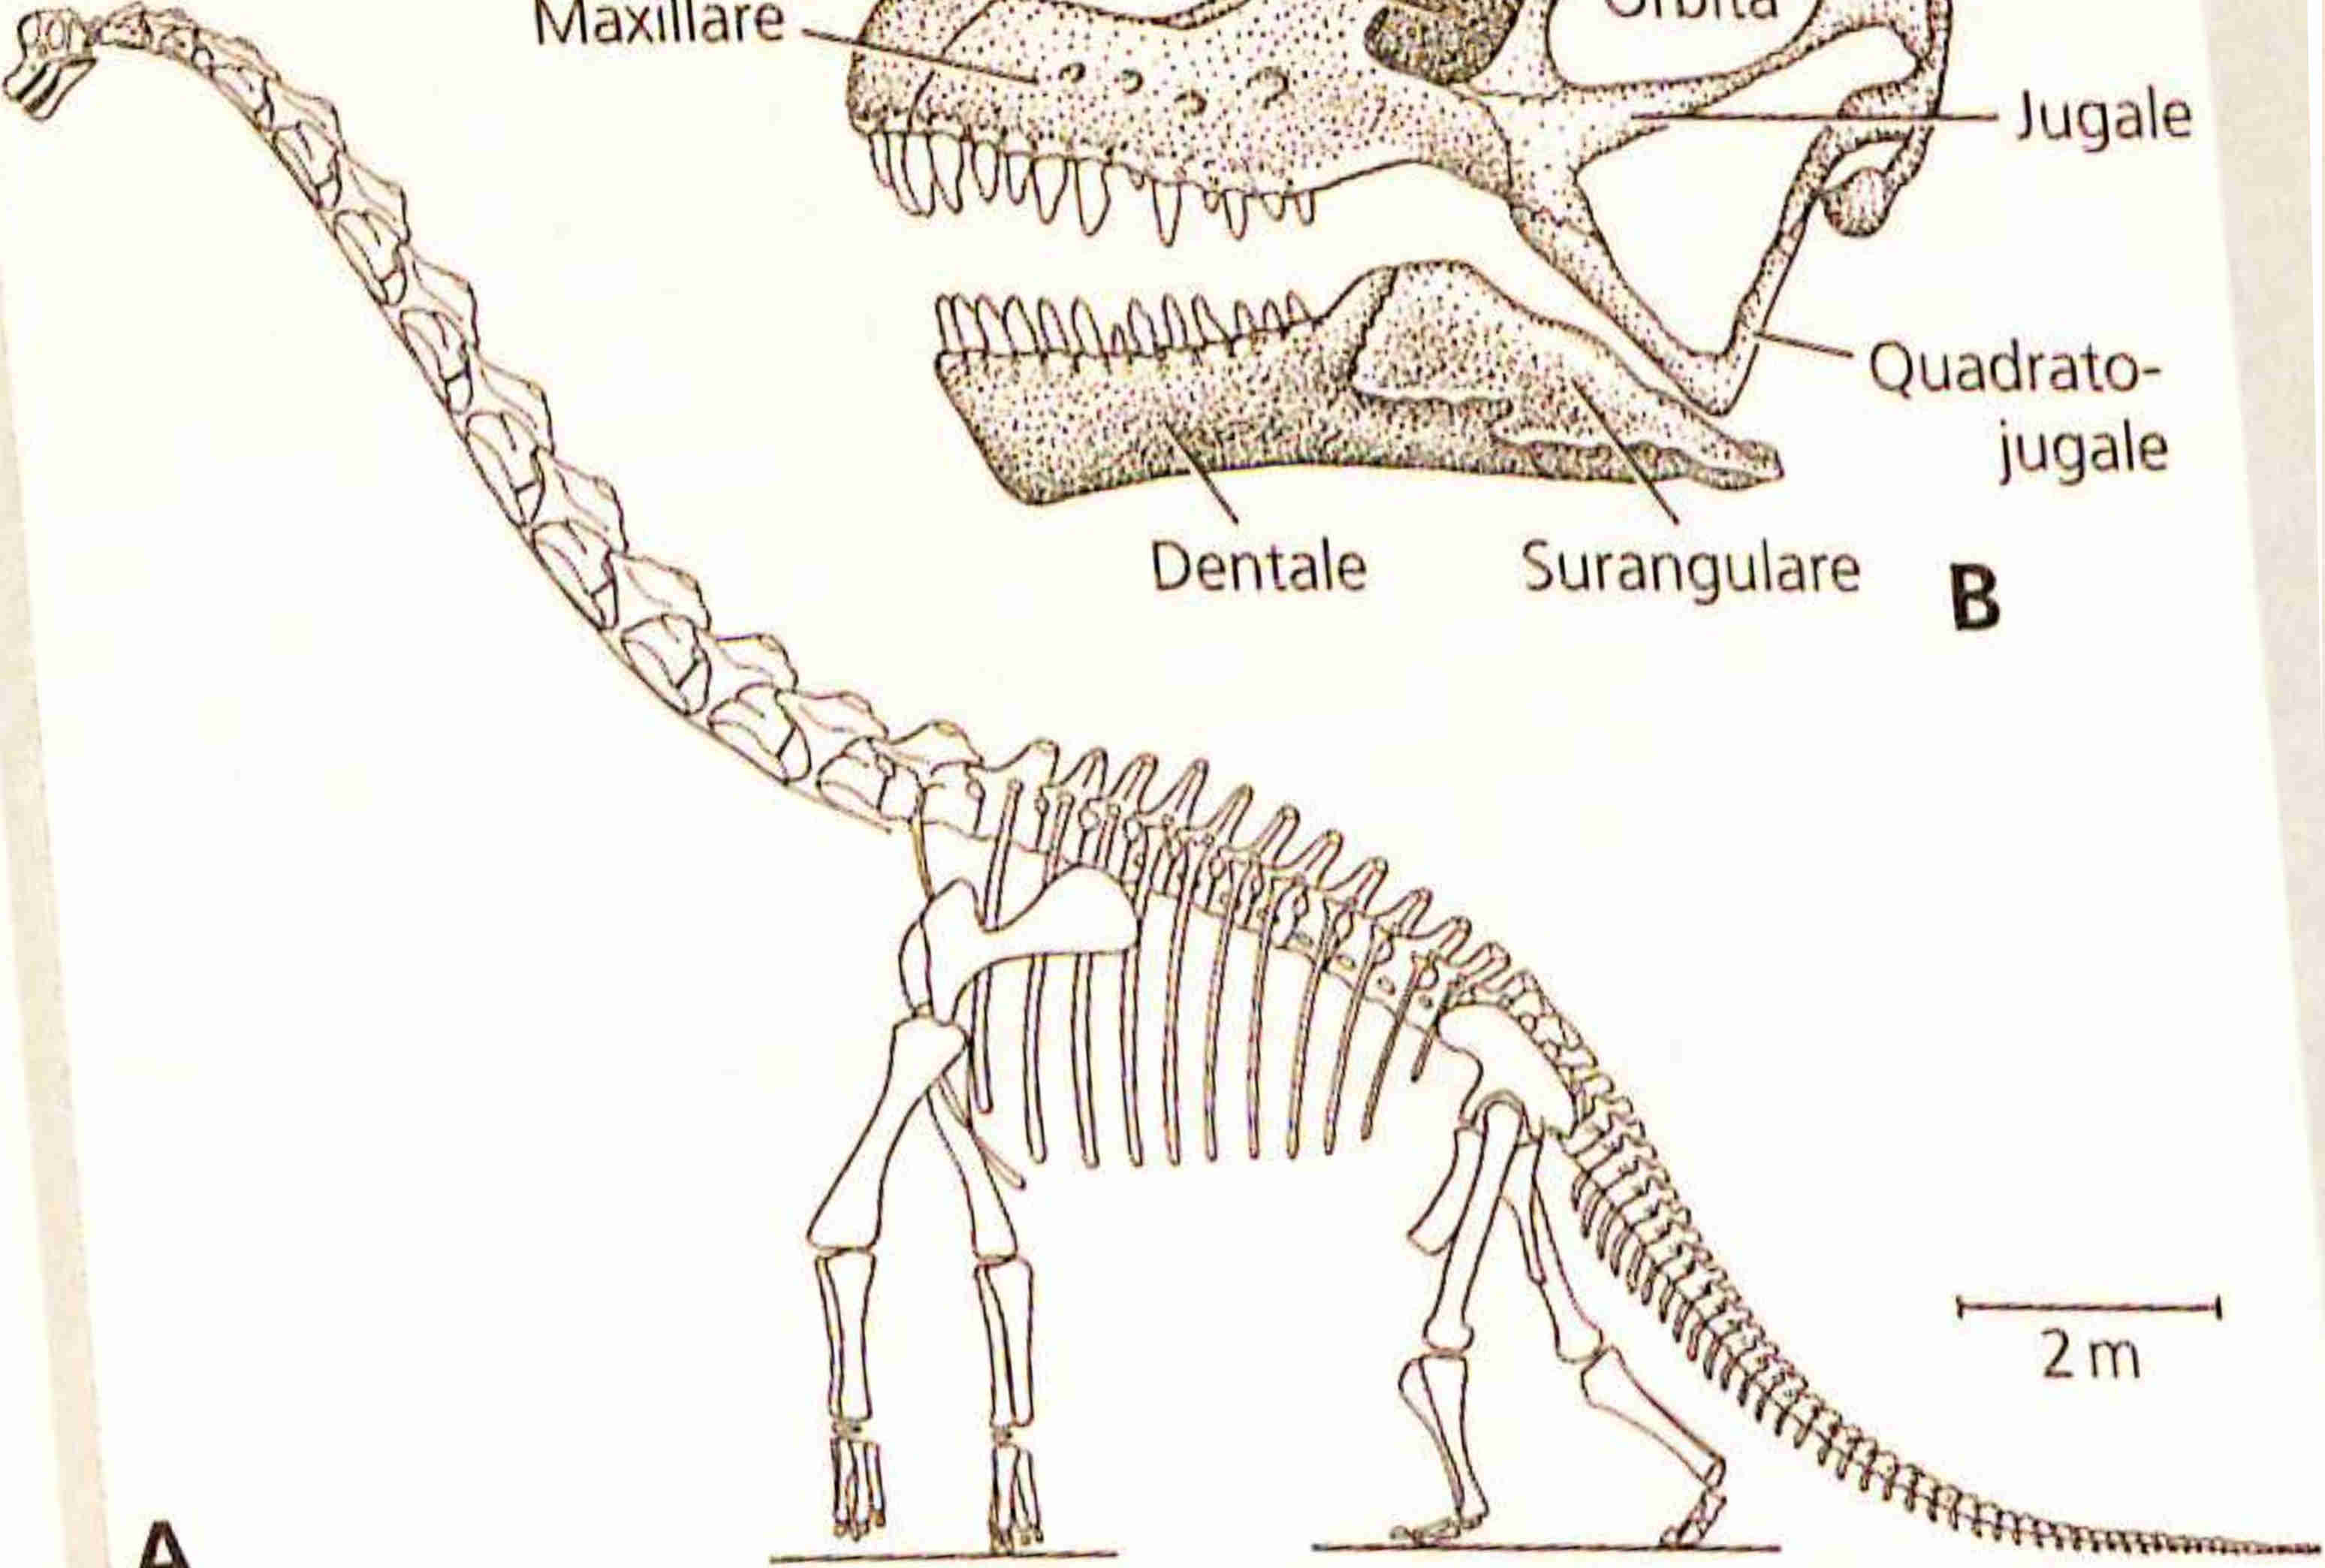
\includegraphics[width=0.2\textwidth]{../PCA/Skelettbilder_klein/Brachiosaurus.jpg}}
\\
\subfloat[Chamäleon]{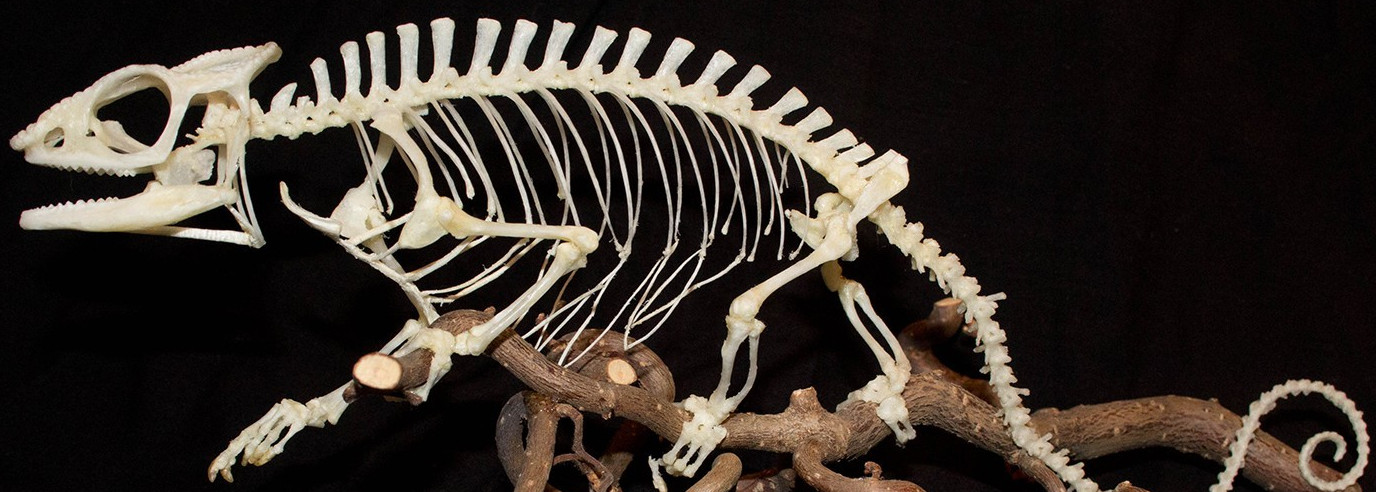
\includegraphics[width=0.2\textwidth]{../PCA/Skelettbilder_klein/Chamaeleon.jpg}}~
\subfloat[Dimetrodon]{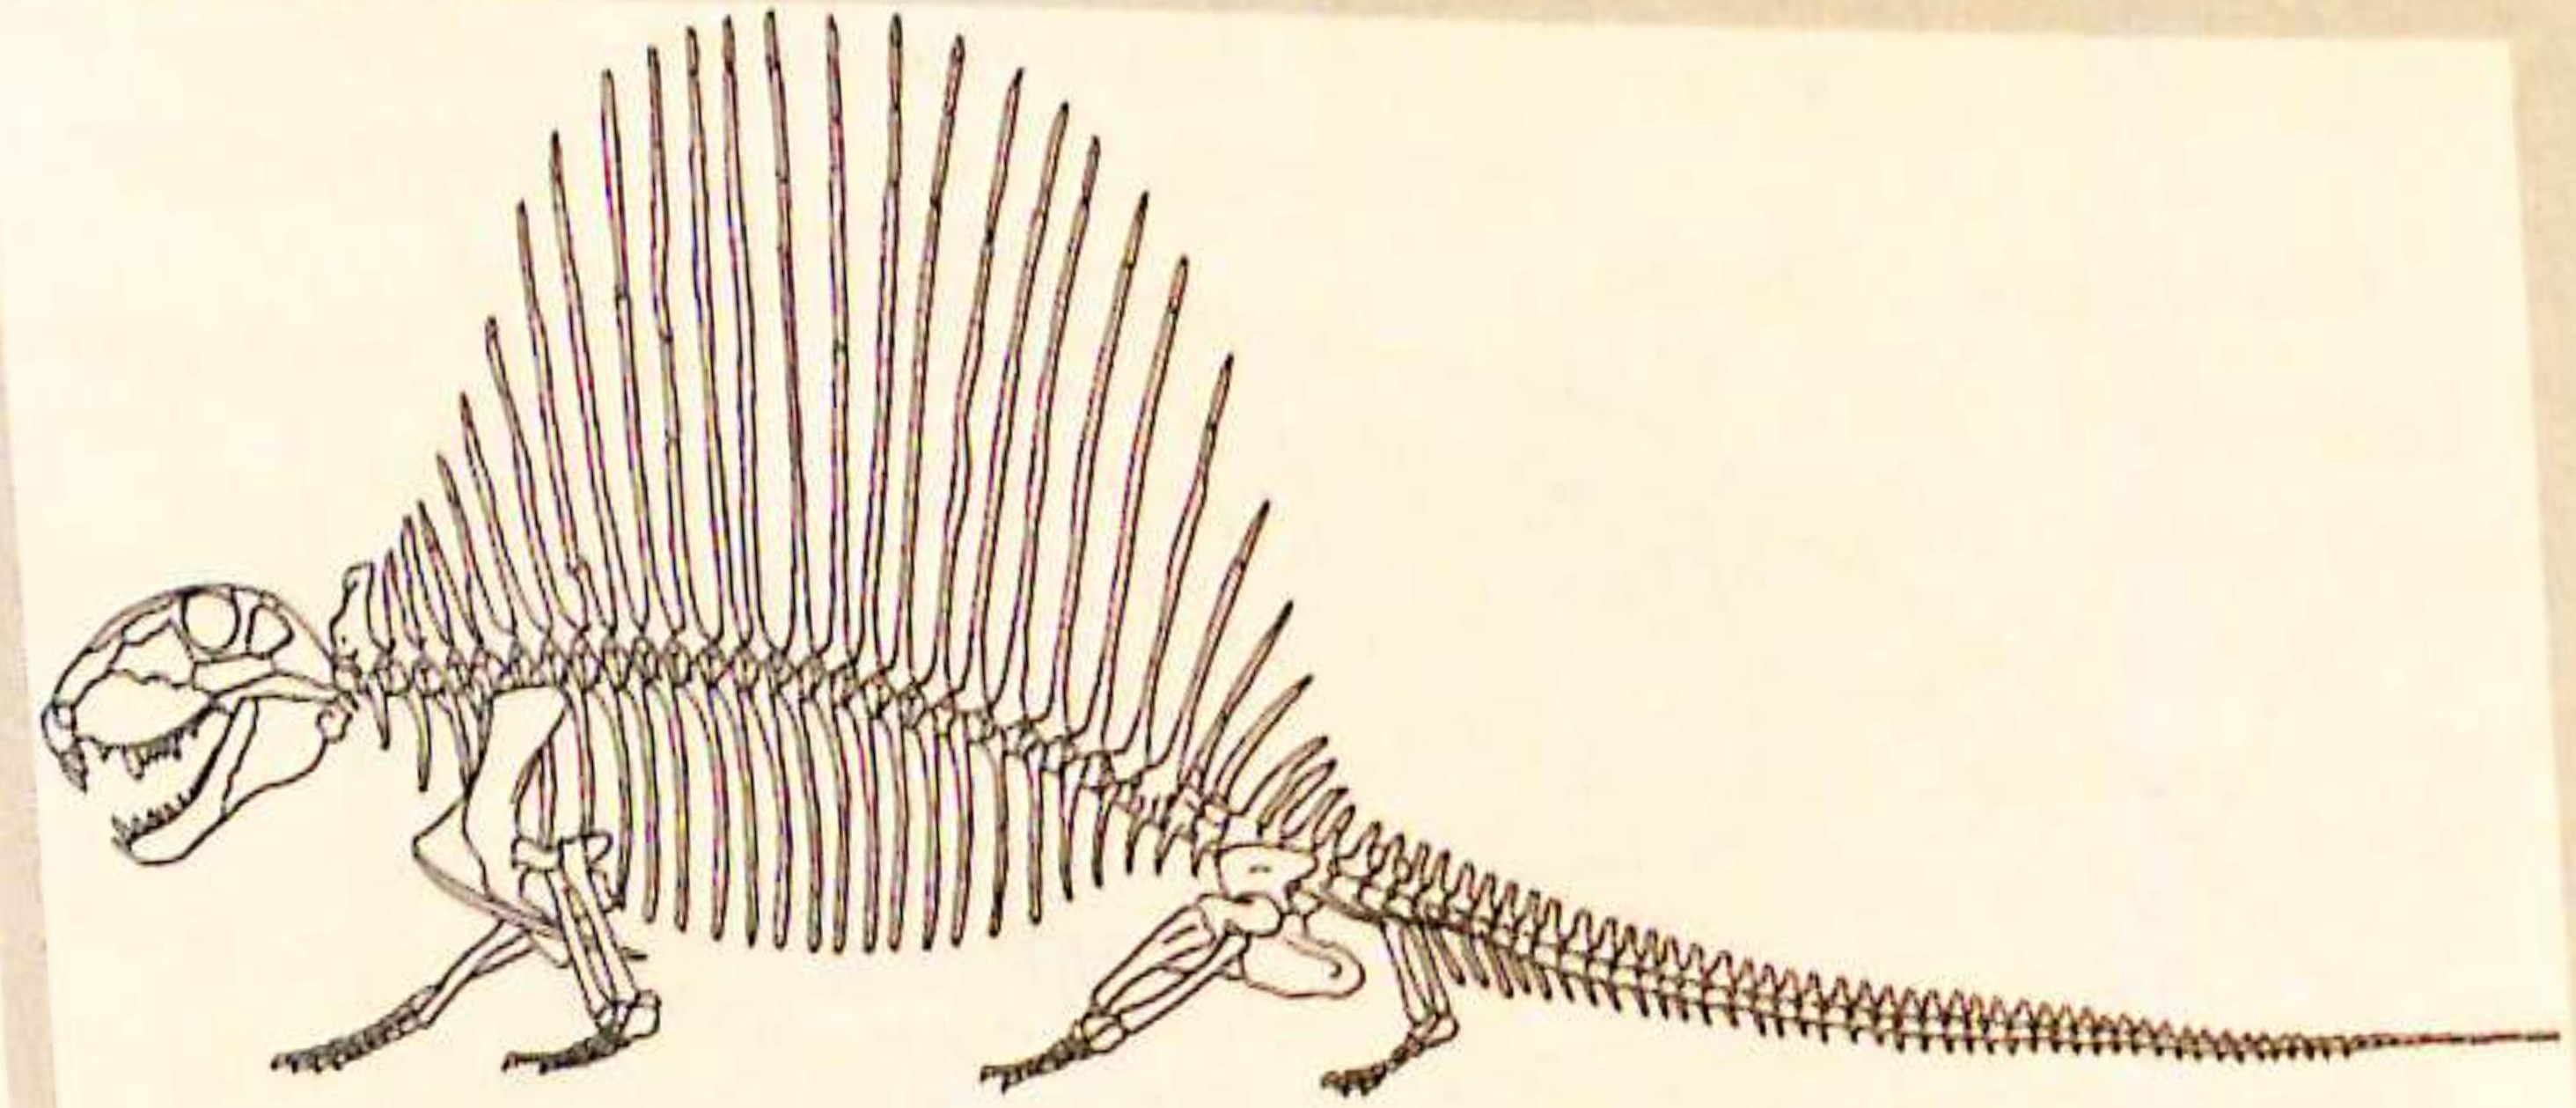
\includegraphics[width=0.2\textwidth]{../PCA/Skelettbilder_klein/Dimetrodon.jpg}}~
\subfloat[Dromedar]{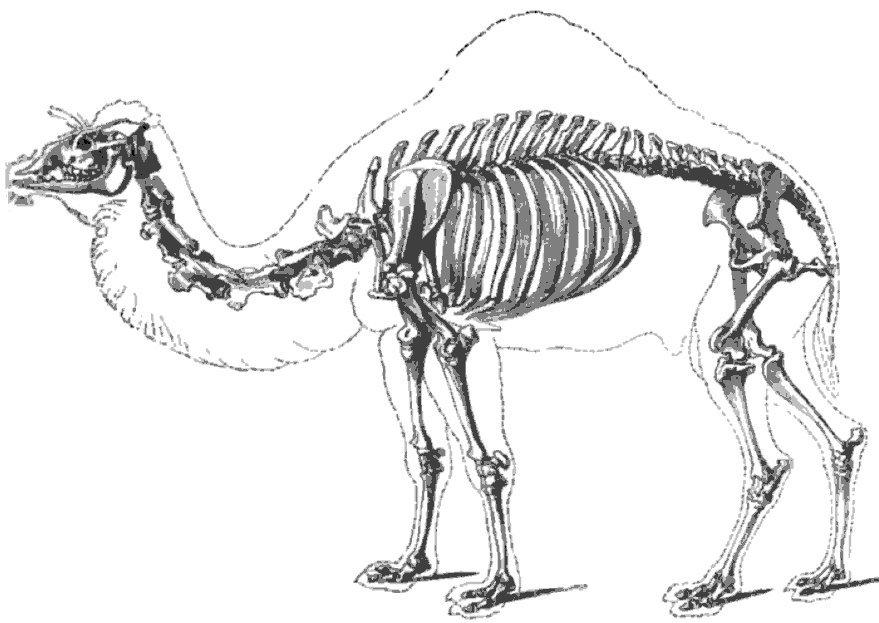
\includegraphics[width=0.2\textwidth]{../PCA/Skelettbilder_klein/Dromedar.jpg}}~
\subfloat[Elster]{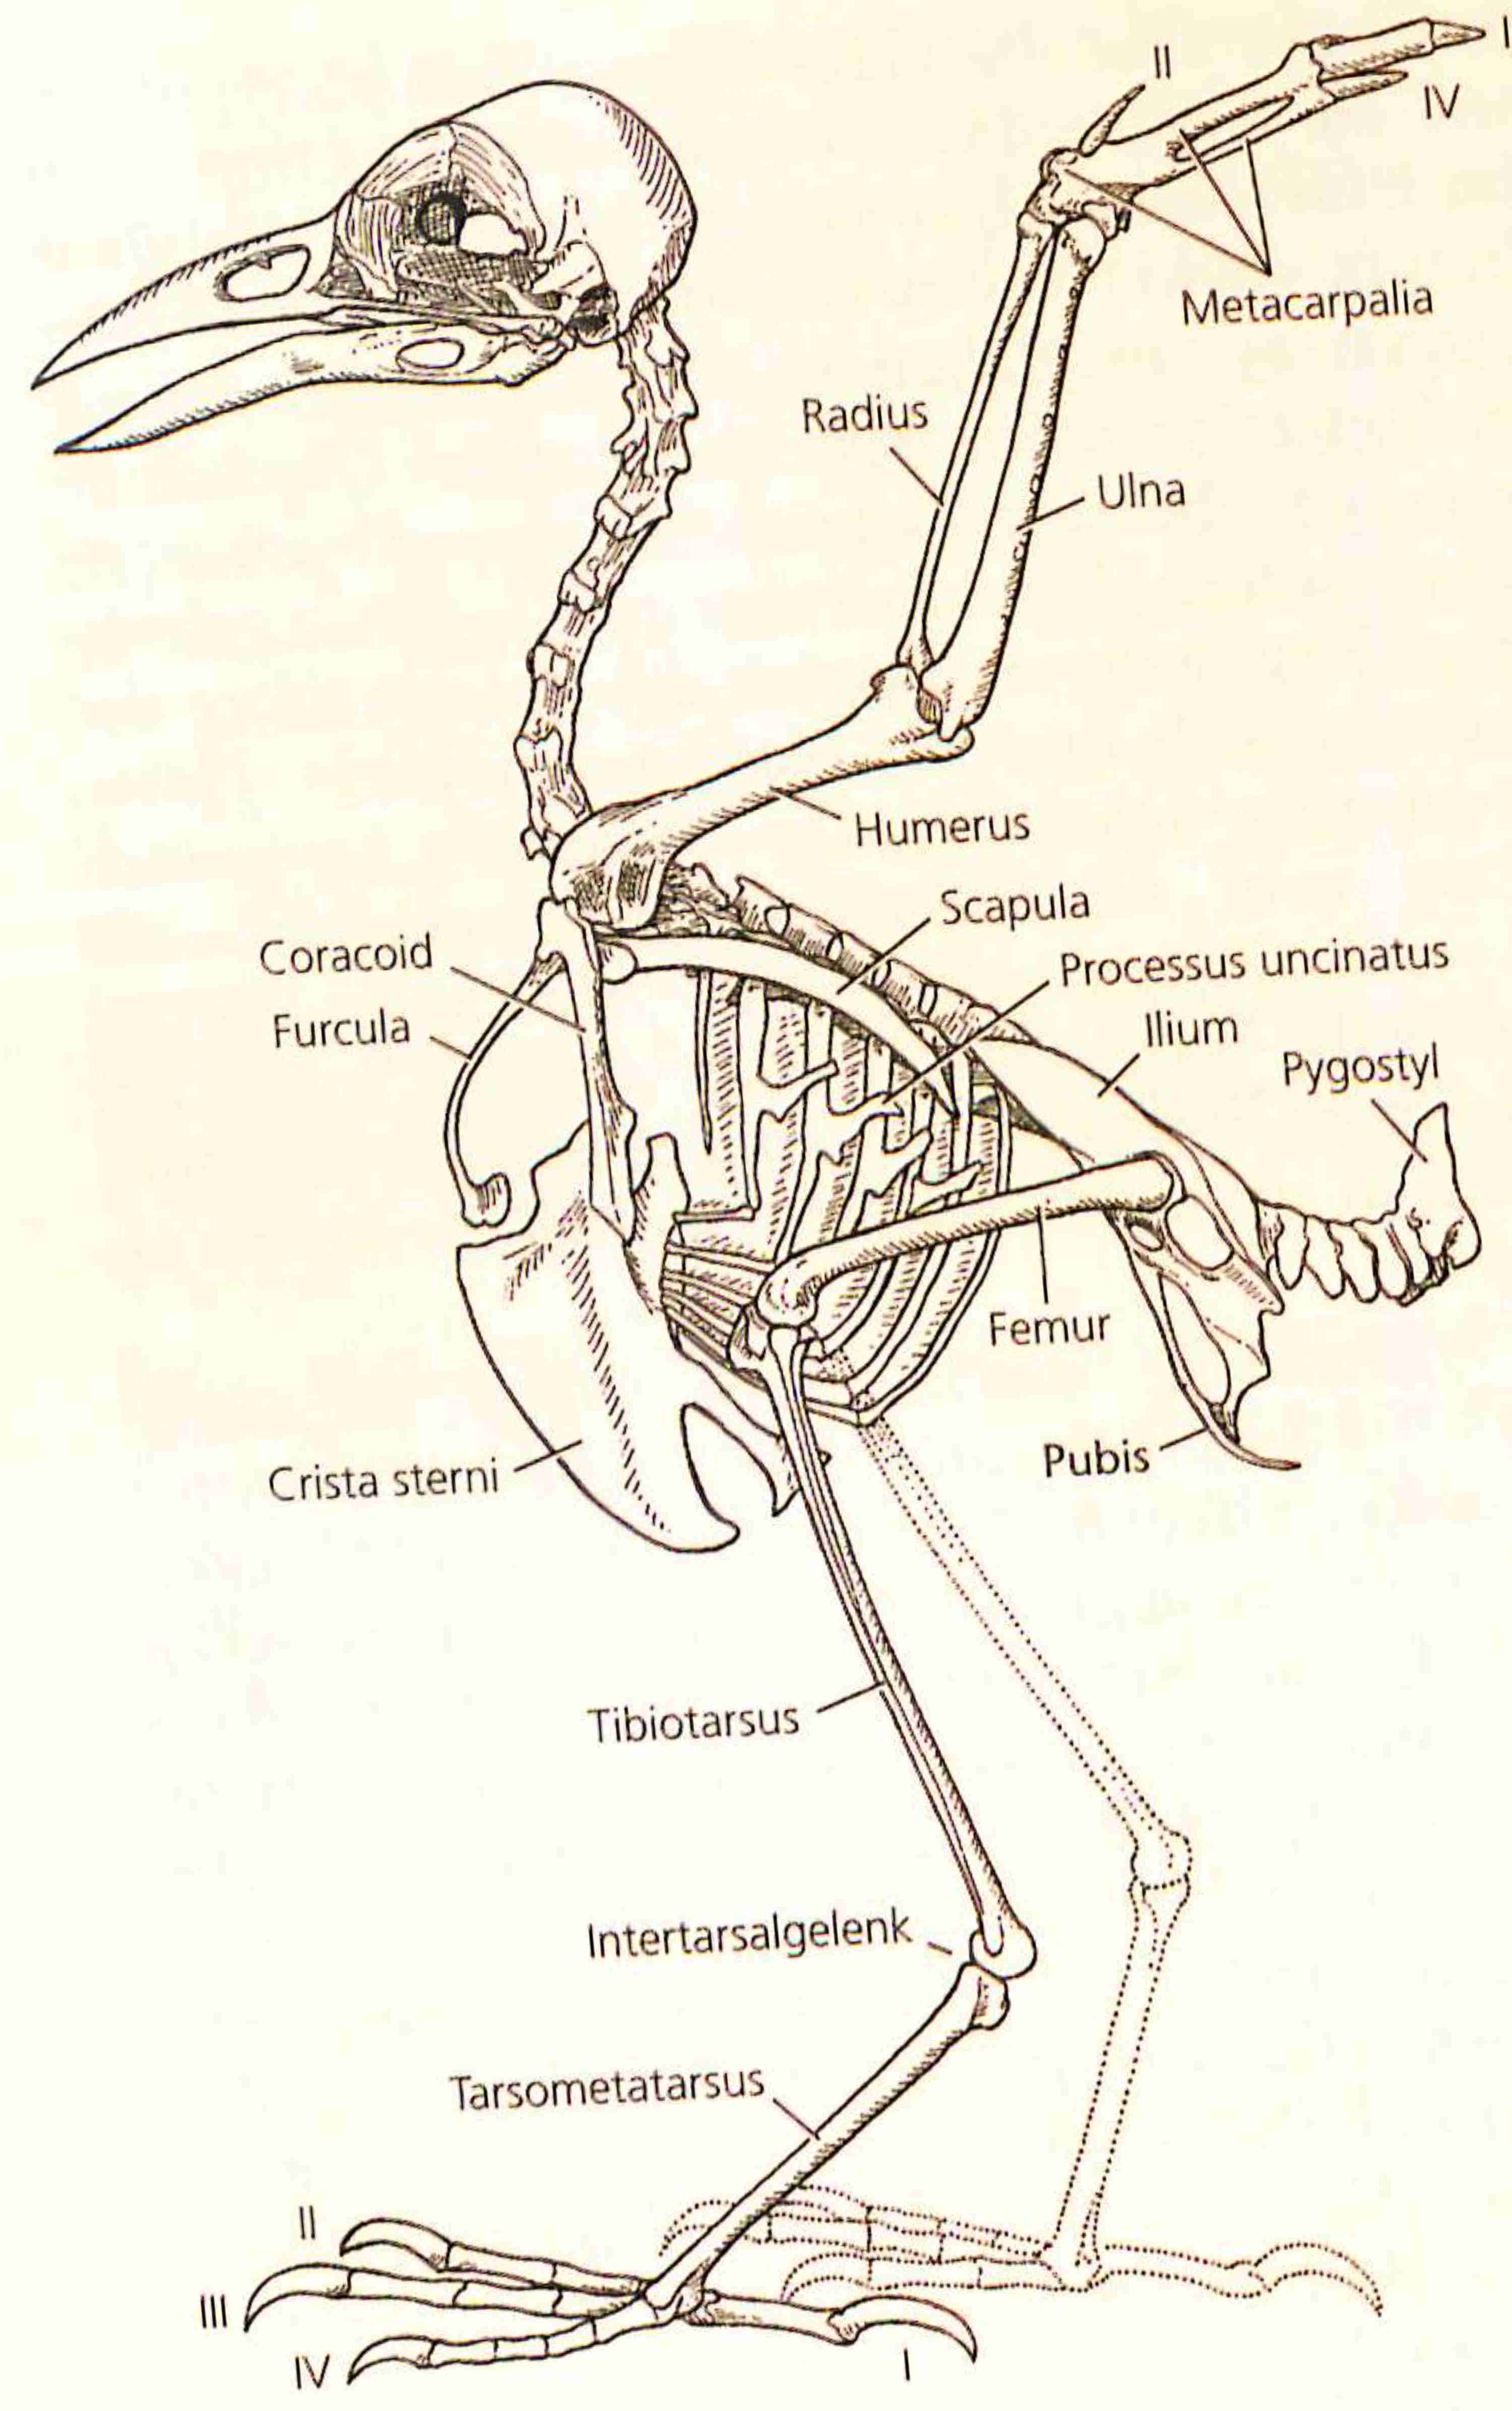
\includegraphics[width=0.2\textwidth]{../PCA/Skelettbilder_klein/Elster.jpg}}~
\subfloat[Forelle]{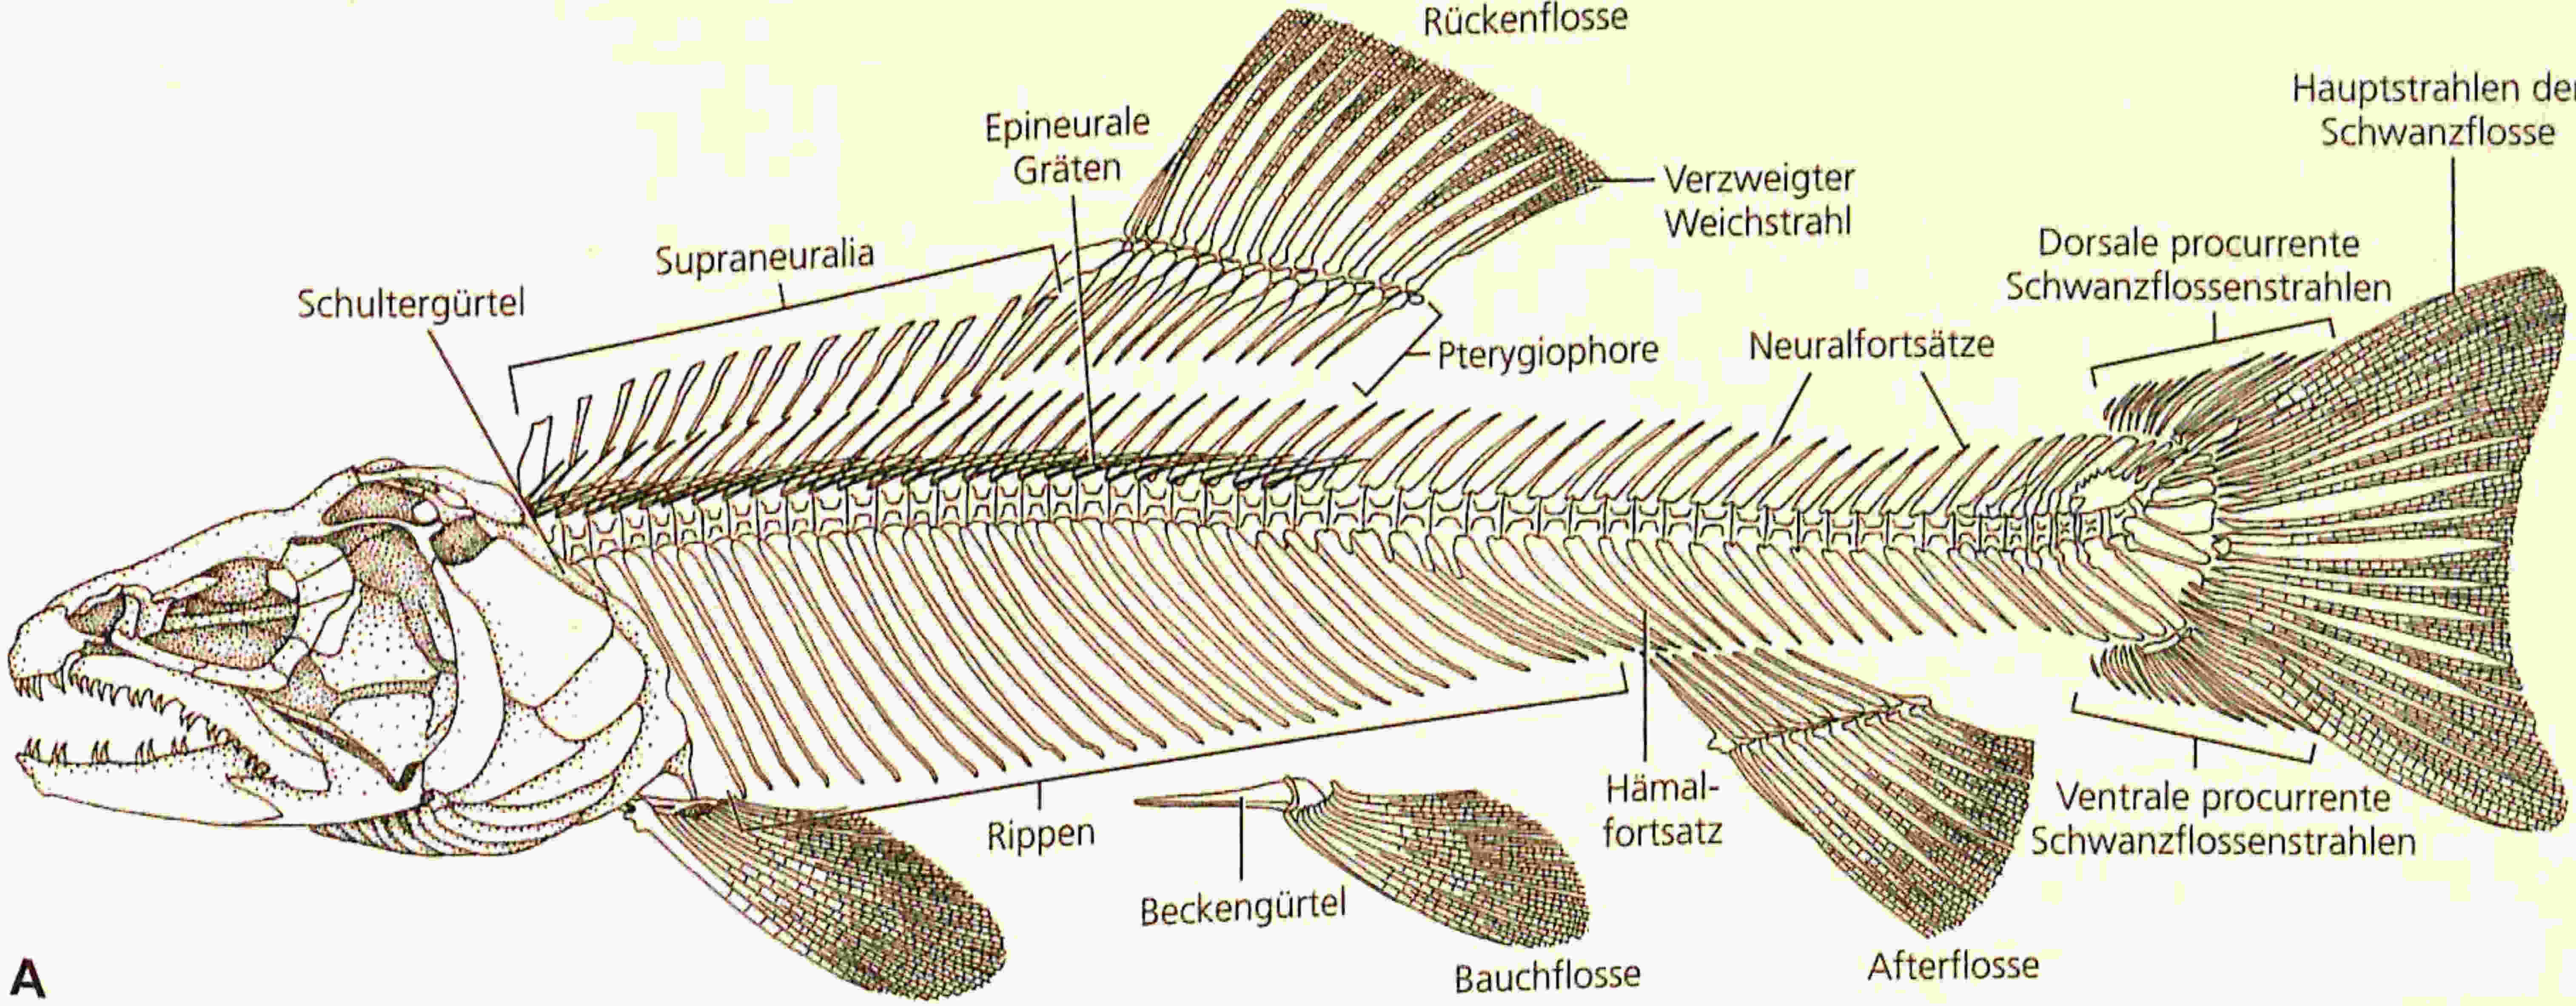
\includegraphics[width=0.2\textwidth]{../PCA/Skelettbilder_klein/Forelle.jpg}}
\\
\subfloat[Frosch]{\includegraphics[width=0.2\textwidth]{../PCA/Skelettbilder_klein/Frosch.jpg}}~
\subfloat[Gämse]{\includegraphics[width=0.2\textwidth]{../PCA/Skelettbilder_klein/Gaemse.jpg}}~
\subfloat[Giraffe]{\includegraphics[width=0.2\textwidth]{../PCA/Skelettbilder_klein/Giraffe.jpg}}~
\subfloat[Gnu]{\includegraphics[width=0.2\textwidth]{../PCA/Skelettbilder_klein/Gnu.jpg}}~
\subfloat[Grönlandwal]{\includegraphics[width=0.2\textwidth]{../PCA/Skelettbilder_klein/Groenlandwal.jpg}}
\\
\subfloat[Ichthyornis]{\includegraphics[width=0.2\textwidth]{../PCA/Skelettbilder_klein/Ichthyornis.jpg}}~
\subfloat[Ichthyosaurus]{\includegraphics[width=0.2\textwidth]{../PCA/Skelettbilder_klein/Ichthyosaurus.jpg}}~
\subfloat[Ichthyostega]{\includegraphics[width=0.2\textwidth]{../PCA/Skelettbilder_klein/Ichthyostega.jpg}}~
\subfloat[Känguru]{\includegraphics[width=0.2\textwidth]{../PCA/Skelettbilder_klein/Kaenguru.jpg}}~
\subfloat[Kaffernbüffel]{\includegraphics[width=0.2\textwidth]{../PCA/Skelettbilder_klein/Kaffernbueffel.jpg}}
\\
\subfloat[Kaninchen]{\includegraphics[width=0.2\textwidth]{../PCA/Skelettbilder_klein/Kaninchen.jpg}}~
\subfloat[Klippschliefer]{\includegraphics[width=0.2\textwidth]{../PCA/Skelettbilder_klein/Klippschliefer.jpg}}~
\subfloat[Koboldmaki]{\includegraphics[width=0.2\textwidth]{../PCA/Skelettbilder_klein/Koboldmaki.jpg}}~
\subfloat[Krokodil]{\includegraphics[width=0.2\textwidth]{../PCA/Skelettbilder_klein/Krokodil.jpg}}~
\subfloat[Landschildkröte]{\includegraphics[width=0.2\textwidth]{../PCA/Skelettbilder_klein/Landschildkroete.jpg}}
\phantomcaption

\end{figure}
\begin{figure}
\ContinuedFloat

\subfloat[Ohrenrobbe]{\includegraphics[width=0.2\textwidth]{../PCA/Skelettbilder_klein/Ohrenrobbe.jpg}}~
\subfloat[Panzerspitzmaus]{\includegraphics[width=0.2\textwidth]{../PCA/Skelettbilder_klein/Panzerspitzmaus.jpg}}~
\subfloat[Parasaurolophus walkeri]{\includegraphics[width=0.2\textwidth]{../PCA/Skelettbilder_klein/Parasaurolophus_walkeri.jpg}}~
\subfloat[Peloneustes philarchus]{\includegraphics[width=0.2\textwidth]{../PCA/Skelettbilder_klein/Peloneustes_philarchus.jpg}}~
\subfloat[Pferd]{\includegraphics[width=0.2\textwidth]{../PCA/Skelettbilder_klein/Pferd.jpg}}
\\
\subfloat[Pottwal]{\includegraphics[width=0.2\textwidth]{../PCA/Skelettbilder_klein/Pottwal.jpg}}~
\subfloat[Rothirsch]{\includegraphics[width=0.2\textwidth]{../PCA/Skelettbilder_klein/Rothirsch.jpg}}~
\subfloat[Schwan]{\includegraphics[width=0.2\textwidth]{../PCA/Skelettbilder_klein/Schwan.jpg}}~
\subfloat[Schwein]{\includegraphics[width=0.2\textwidth]{../PCA/Skelettbilder_klein/Schwein.jpg}}~
\subfloat[Seehund]{\includegraphics[width=0.2\textwidth]{../PCA/Skelettbilder_klein/Seehund.jpg}}
\\
\subfloat[Sinornis]{\includegraphics[width=0.2\textwidth]{../PCA/Skelettbilder_klein/Sinornis.jpg}}~
\subfloat[Stegosaurus]{\includegraphics[width=0.2\textwidth]{../PCA/Skelettbilder_klein/Stegosaurus.jpg}}~
\subfloat[Strauss]{\includegraphics[width=0.2\textwidth]{../PCA/Skelettbilder_klein/Strauss.jpg}}~
\subfloat[Taube]{\includegraphics[width=0.2\textwidth]{../PCA/Skelettbilder_klein/Taube.jpg}}~
\subfloat[Thrinaxodon]{\includegraphics[width=0.2\textwidth]{../PCA/Skelettbilder_klein/Thrinaxodon.jpg}}
\\
\subfloat[Triceratops]{\includegraphics[width=0.2\textwidth]{../PCA/Skelettbilder_klein/Triceratops.jpg}}~
\subfloat[Tyrannosaurus Rex]{\includegraphics[width=0.2\textwidth]{../PCA/Skelettbilder_klein/Tyrannosaurus_Rex.jpg}}~
\subfloat[Urpferdchen]{\includegraphics[width=0.2\textwidth]{../PCA/Skelettbilder_klein/Urpferdchen.jpg}}


\caption{Alle Bilder, die als Eingabe für die PCA verwendet wurden.}
\label{all_images}
\end{figure}


 
 \subsection{Gewichte}
 \label{appendix_pca_weight}
 
 \begin{itemize}
  \item Afrikanischer Elefant 4000kg, \url{https://de.upali.ch/gewicht-und-grosse/}
  \item Afrikanischer Strauß bis 135kg, \url{https://de.wikipedia.org/wiki/Afrikanischer_Strau\%C3\%9F}
  \item Amerikanischer Flussbarsch 2kg, \url{http://tierdoku.com/index.php?title=Amerikanischer_Flussbarsch}
  \item Archaeopteryx 1kg, \url{https://de.wikipedia.org/wiki/Archaeopteryx}
  \item Blauwal 120 Tonnen, \url{http://tierdoku.com/index.php?title=Blauwal}, "`das schwerste bekannte Tier der Erdgeschichte"' \url{https://de.wikipedia.org/wiki/Blauwal}
  \item Brachiosaurus 23-44 Tonnen, \url{https://de.wikipedia.org/wiki/Brachiosaurus}
  \item Chamäleon 0,1-2kg, \url{https://www.tierchenwelt.de/echsen/128-chamaeleon.html}
  \item Dimetrodon 250kg, \url{https://de.wikipedia.org/wiki/Dimetrodon}
  \item Dromedar 300-700kg, \url{https://de.wikipedia.org/wiki/Dromedar}
  \item Durschnittsgewicht (Warmblut-)Pferd 600 kg, \url{https://www.reitarena.com/de/blog/blog-post/2015/03/03/das-pferd-grundlegende-fakten.html}
  \item Elster 0,2kg, \url{https://de.wikipedia.org/wiki/Elster}
  \item Forelle 10-50kg (je nach Art), \url{https://de.wikipedia.org/wiki/Forelle}
  \item Frosch 10g, \url{http://www.biologie-schule.de/frosch-steckbrief.php}
  \item Gämse 25-50kg, \url{https://de.wikipedia.org/wiki/G\%C3\%A4mse}
  \item Girafffe bis 2 Tonnen, \url{https://www.tierchenwelt.de/huftiere/73-giraffe.html}
  \item Gnu 140-250kg, \url{https://de.wikipedia.org/wiki/Gnus}
  \item Grönlandwal 50-100 Tonnen, \url{https://de.wikipedia.org/wiki/Gr\%C3\%B6nlandwal}
  \item Ichthyornis 0.3kg, \url{http://dinodata.de/animals/birds/pages_i/ichthyornis.php}
  \item Ichthyosaurus 90kg, \url{https://www.tiere-online.de/sonstige-tiere/dinosaurier/ichthyosaurus/}
  \item Ichthyostega 80kg, \url{https://dinosaurierwelt.com/ichthyostega/}
  \item Kaffernbüffel 350-900kg, \url{https://de.wikipedia.org/wiki/Kaffernb\%C3\%BCffel}
  \item Känguru 2-90kg ,\url{https://de.wikipedia.org/wiki/K\%C3\%A4ngurus}
  \item Kaninchen je nach Art, ganz grob 1kg
  \item Klippschliefer 2-5kg, \url{https://de.wikipedia.org/wiki/Klippschliefer}
  \item Koboldmaki 0,1kg, \url{https://de.wikipedia.org/wiki/Koboldmakis}
  \item Krokodil 100-1000kg, \url{https://de.wikipedia.org/wiki/Krokodile}
  \item Landschildkröte je nach Art, grob 50kg
  \item Ohrenrobbe 25-500kg, \url{https://de.wikipedia.org/wiki/Ohrenrobben}
  \item Panzerspitzmaus 100g ,\url{https://de.wikipedia.org/wiki/Panzerspitzmaus}
  \item Parasaurolophus walkeri 4-5 Tonnen, \url{http://tierdoku.com/index.php?title=Parasaurolophus_walkeri}
  \item Peloneustes philarchus 100kg, \url{https://de.wikipedia.org/wiki/Peloneustes}
  \item Pottwal bis 50 Tonnen, \url{https://de.wikipedia.org/wiki/Pottwal}
  \item Rothirsch 80-350kg, \url{https://de.wikipedia.org/wiki/Rothirsch}
  \item Schlange bis 100kg bei Riesenschlangen, \url{https://de.wikipedia.org/wiki/Schlangen}
  \item Schwan 14kg, \url{https://de.wikipedia.org/wiki/Schw\%C3\%A4ne}
  \item Schwein 100kg, \url{https://de.wikipedia.org/wiki/Hausschwein}
  \item Seehund 100-150kg, \url{https://de.wikipedia.org/wiki/Seehund}
  \item Sinornis 20g, \url{http://dinodata.de/animals/birds/pages_s/sinornis.php}
  \item Stegosaurus 4,5 Tonnen, \url{https://de.wikipedia.org/wiki/Stegosaurus}
  \item Taube je nach Art, grob 1-2kg
  \item Thrinaxodon Reptil "`ein paar Pfund"', \url{https://www.thoughtco.com/thrinaxodon-1091887}
  \item Triceratops 6-12 Tonnen, \url{https://de.wikipedia.org/wiki/Triceratops}
  \item Tyrannosaurus 9 Tonnen, \url{https://de.wikipedia.org/wiki/Tyrannosaurus}
  \item Urpferdchen (Propalaeotherium) 30kg, \url{https://de.wikipedia.org/wiki/Propalaeotherium}
 \end{itemize}
 

% --------------
% Erhobene Werte
% --------------

  \begin{figure}
   \subfloat[Erster Punkt des Halses]{\includegraphics[width=0.3\textwidth]{../PCA/gnuplot/results_with_leg_tag/input_neck1.pdf}}
   \qquad
   \subfloat[Zweiter Punkt des Halses]{\includegraphics[width=0.3\textwidth]{../PCA/gnuplot/results_with_leg_tag/input_neck2.pdf}}
   \qquad
   \subfloat[Dritter Punkt des Halses]{\includegraphics[width=0.3\textwidth]{../PCA/gnuplot/results_with_leg_tag/input_neck3.pdf}}
   \\
   \subfloat[Vierter Punkt des Halses \bzw erster Punkt des Rückens]{\includegraphics[width=0.3\textwidth]{../PCA/gnuplot/results_with_leg_tag/input_back1.pdf}}
   \qquad
   \subfloat[Zweiter Punkt des Rückens]{\includegraphics[width=0.3\textwidth]{../PCA/gnuplot/results_with_leg_tag/input_back2.pdf}}
   \qquad
   \subfloat[Dritter Punkt des Rückens]{\includegraphics[width=0.3\textwidth]{../PCA/gnuplot/results_with_leg_tag/input_back3.pdf}}
   \\
   \subfloat[Vierter Punkt des Rückens \bzw erster Punkt des Schwanzes]{\includegraphics[width=0.3\textwidth]{../PCA/gnuplot/results_with_leg_tag/input_back4.pdf}}
   \qquad
   \subfloat[Zweiter Punkt des Schwanzes]{\includegraphics[width=0.3\textwidth]{../PCA/gnuplot/results_with_leg_tag/input_tail2.pdf}}
   \qquad
   \subfloat[Dritter Punkt des Schwanzes]{\includegraphics[width=0.3\textwidth]{../PCA/gnuplot/results_with_leg_tag/input_tail3.pdf}}
   \\
   \subfloat[Vierter Punkt des Schwanzes]{\includegraphics[width=0.3\textwidth]{../PCA/gnuplot/results_with_leg_tag/input_tail4.pdf}}
   \qquad
   \subfloat[Länge Ober- und Unterarm]{\includegraphics[width=0.3\textwidth]{../PCA/gnuplot/results_with_leg_tag/input_upper+lowerArm.pdf}}
   \qquad
   \subfloat[Länge Unterarm und Hand]{\includegraphics[width=0.3\textwidth]{../PCA/gnuplot/results_with_leg_tag/input_lowerArm+hand.pdf}}
   \phantomcaption
  \end{figure}
  \begin{figure}
   \ContinuedFloat
   \subfloat[Länge Ober- und Unterschenkel]{\includegraphics[width=0.3\textwidth]{../PCA/gnuplot/results_with_leg_tag/input_upper+lowerLeg.pdf}}
   \qquad
   \subfloat[Länge Unterschenkel und Fuß]{\includegraphics[width=0.3\textwidth]{../PCA/gnuplot/results_with_leg_tag/input_lowerLeg+foot.pdf}}
   
   \caption{Erhobene Daten: Punkte der Bézierkurven der Wirbelsäule und Längen der Extremitäten. Bei den Extremitäten ist jeweils gegeneinander abgetragen Ober- und Unterarm, Ober- und Unterschenkel, Unterarm und Hand, Unterschenkel und Fuß. Markiert ist jeweils ob die Datenpunkte $0$ (rot), $2$ (blau) oder $4$ (grün) Beine haben.}
   \label{input_data}
  \end{figure}
  
 \begin{figure}
  \subfloat[lineare Skala]{\includegraphics[width=0.5\textwidth]{../PCA/gnuplot/results_with_leg_tag/input_weight.pdf} \label{gnuplot_weight}}
  \qquad
  \subfloat[logarithmische Skala]{\includegraphics[width=0.5\textwidth]{../PCA/gnuplot/results_with_leg_tag/input_weight_logarithmic.pdf}\label{gnuplot_log_weight}}
  
  \caption{Erhobene Daten: Gewicht. Markiert ist jeweils ob die Datenpunkte $0$ (rot), $2$ (blau) oder $4$ (grün) Beine haben.}
  \label{input_data_weight}
 \end{figure}
 
 %--------------
 % QQ Diagramme
 % ------------

  \begin{figure}
   \subfloat[Erster Punkt des Halses, x-Koordinate]{\includegraphics[width=0.3\textwidth]{../PCA/gnuplot/results_qq_diagrams/QQ_diagram0.pdf}}
   \qquad
   \subfloat[Erster Punkt des Halses, y-Koordinate]{\includegraphics[width=0.3\textwidth]{../PCA/gnuplot/results_qq_diagrams/QQ_diagram1.pdf}}
   \qquad
   \subfloat[Zweiter Punkt des Halses, x-Koordinate]{\includegraphics[width=0.3\textwidth]{../PCA/gnuplot/results_qq_diagrams/QQ_diagram2.pdf}}
   \\
   \subfloat[Zweiter Punkt des Halses, y-Koordinate]{\includegraphics[width=0.3\textwidth]{../PCA/gnuplot/results_qq_diagrams/QQ_diagram3.pdf}}
   \qquad
   \subfloat[Dritter Punkt des Halses, x-Koordinate]{\includegraphics[width=0.3\textwidth]{../PCA/gnuplot/results_qq_diagrams/QQ_diagram4.pdf}}
   \qquad
   \subfloat[Dritter Punkt des Halses, y-Koordinate]{\includegraphics[width=0.3\textwidth]{../PCA/gnuplot/results_qq_diagrams/QQ_diagram5.pdf}}
   \\
   \subfloat[Erster Punkt des Rückens, x-Koordinate]{\includegraphics[width=0.3\textwidth]{../PCA/gnuplot/results_qq_diagrams/QQ_diagram6.pdf}}
   \qquad
   \subfloat[Erster Punkt des Rückens, y-Koordinate]{\includegraphics[width=0.3\textwidth]{../PCA/gnuplot/results_qq_diagrams/QQ_diagram7.pdf}}
   \qquad
   \subfloat[Zweiter Punkt des Rückens, x-Koordinate]{\includegraphics[width=0.3\textwidth]{../PCA/gnuplot/results_qq_diagrams/QQ_diagram8.pdf}}
   \\
   \subfloat[Zweiter Punkt des Rückens, y-Koordinate]{\includegraphics[width=0.3\textwidth]{../PCA/gnuplot/results_qq_diagrams/QQ_diagram9.pdf}}
   \qquad
   \subfloat[Dritter Punkt des Rückens, x-Koordinate]{\includegraphics[width=0.3\textwidth]{../PCA/gnuplot/results_qq_diagrams/QQ_diagram10.pdf}}
   \qquad
   \subfloat[Dritter Punkt des Rückens, y-Koordinate]{\includegraphics[width=0.3\textwidth]{../PCA/gnuplot/results_qq_diagrams/QQ_diagram11.pdf}}
   \phantomcaption
  \end{figure}
  \begin{figure}
   \ContinuedFloat
   \subfloat[Vierter Punkt des Rückens, x-Koordinate]{\includegraphics[width=0.3\textwidth]{../PCA/gnuplot/results_qq_diagrams/QQ_diagram12.pdf}}
   \qquad
   \subfloat[Vierter Punkt des Rückens, y-Koordinate]{\includegraphics[width=0.3\textwidth]{../PCA/gnuplot/results_qq_diagrams/QQ_diagram13.pdf}}
   \qquad
   \subfloat[Zweiter Punkt des Schwanzes, x-Koordinate]{\includegraphics[width=0.3\textwidth]{../PCA/gnuplot/results_qq_diagrams/QQ_diagram14.pdf}}
   \\
   \subfloat[Zweiter Punkt des Schwanzes, y-Koordinate]{\includegraphics[width=0.3\textwidth]{../PCA/gnuplot/results_qq_diagrams/QQ_diagram15.pdf}}
   \qquad
   \subfloat[Dritter Punkt des Schwanzes, x-Koordinate]{\includegraphics[width=0.3\textwidth]{../PCA/gnuplot/results_qq_diagrams/QQ_diagram16.pdf}}
   \qquad
   \subfloat[Dritter Punkt des Schwanzes, y-Koordinate]{\includegraphics[width=0.3\textwidth]{../PCA/gnuplot/results_qq_diagrams/QQ_diagram17.pdf}}
   \\
   \subfloat[Vierter Punkt des Schwanzes, x-Koordinate]{\includegraphics[width=0.3\textwidth]{../PCA/gnuplot/results_qq_diagrams/QQ_diagram18.pdf}}
   \qquad
   \subfloat[Vierter Punkt des Schwanzes, y-Koordinate]{\includegraphics[width=0.3\textwidth]{../PCA/gnuplot/results_qq_diagrams/QQ_diagram19.pdf}}
   
   \caption{Quantil-Quantil-Diagramme für alle Dimensionen der Wirbelsäule}
   \label{qq_diagrams_spine}
  \end{figure}
  \begin{figure}
   \subfloat[Länge Oberarm]{\includegraphics[width=0.3\textwidth]{../PCA/gnuplot/results_qq_diagrams/QQ_diagram22.pdf}}
   \qquad
   \subfloat[Länge Unterarm]{\includegraphics[width=0.3\textwidth]{../PCA/gnuplot/results_qq_diagrams/QQ_diagram23.pdf}}
   \qquad
   \subfloat[Länge Hand]{\includegraphics[width=0.3\textwidth]{../PCA/gnuplot/results_qq_diagrams/QQ_diagram24.pdf}}
   \\
   \subfloat[Länge Oberschenkel]{\includegraphics[width=0.3\textwidth]{../PCA/gnuplot/results_qq_diagrams/QQ_diagram25.pdf}}
   \qquad
   \subfloat[Länge Unterschenkel]{\includegraphics[width=0.3\textwidth]{../PCA/gnuplot/results_qq_diagrams/QQ_diagram26.pdf}}
   \qquad
   \subfloat[Länge Fuß]{\includegraphics[width=0.3\textwidth]{../PCA/gnuplot/results_qq_diagrams/QQ_diagram27.pdf}}

   \caption{Quantil-Quantil-Diagramme für die Dimensionen der Eingabedaten, die zusätzlich zur Wirbelsäule erhoben wurden. Nicht dargestellt ist das binäre Attribut \emph{Flügel} und die Anzahl der Beine mit Bodenkontakt.}
   \label{qq_diagrams_rest}
  \end{figure}
  
  
% ----------------------------
% Mit PCA erzeugte Datenpunkte
% ----------------------------
 
 \begin{figure}
   \centering
   \subfloat[1-, \emph{Flügel} $0,38$, \emph{Beine} $1,6$, \emph{Gewicht} $92$kg]{\includegraphics[width=0.45\textwidth]{../PCA/sqrtEV_log_weight_downscaled_wings_legs_and_weight/EV1_neg.jpg}}
   \qquad
   \subfloat[1+, \emph{Flügel} $-0,057$, \emph{Beine} $1,2$, \emph{Gewicht} $94$kg]{\includegraphics[width=0.45\textwidth]{../PCA/sqrtEV_log_weight_downscaled_wings_legs_and_weight/EV1_pos.jpg}}
   \\
   \subfloat[2-, \emph{Flügel} $0,014$, \emph{Beine} $1,4$, \emph{Gewicht} $94$kg]{\includegraphics[width=0.45\textwidth]{../PCA/sqrtEV_log_weight_downscaled_wings_legs_and_weight/EV2_neg.jpg}}
   \qquad
   \subfloat[2+, \emph{Flügel} $0,3$, \emph{Beine} $1,3$, \emph{Gewicht} $93$kg]{\includegraphics[width=0.45\textwidth]{../PCA/sqrtEV_log_weight_downscaled_wings_legs_and_weight/EV2_pos.jpg}}
   \\
   \subfloat[3-, \emph{Flügel} $0,11$, \emph{Beine} $1,6$, \emph{Gewicht} $93$kg]{\includegraphics[width=0.45\textwidth]{../PCA/sqrtEV_log_weight_downscaled_wings_legs_and_weight/EV3_neg.jpg}}
   \qquad
   \subfloat[3+, \emph{Flügel} $0,21$, \emph{Beine} $1,2$, \emph{Gewicht} $93$kg]{\includegraphics[width=0.45\textwidth]{../PCA/sqrtEV_log_weight_downscaled_wings_legs_and_weight/EV3_pos.jpg}}
   \phantomcaption
 \end{figure}
 \begin{figure}
   \ContinuedFloat
   \centering
   \subfloat[4-, \emph{Flügel} $0,3$, \emph{Beine} $1$, \emph{Gewicht} $92$kg]{\includegraphics[width=0.45\textwidth]{../PCA/sqrtEV_log_weight_downscaled_wings_legs_and_weight/EV4_neg.jpg}}
   \qquad
   \subfloat[4+, \emph{Flügel} $0,022$, \emph{Beine} $1,8$, \emph{Gewicht} $94$kg]{\includegraphics[width=0.45\textwidth]{../PCA/sqrtEV_log_weight_downscaled_wings_legs_and_weight/EV4_pos.jpg}}
   \\
   \subfloat[5-, \emph{Flügel} $0,08$, \emph{Beine} $1,6$, \emph{Gewicht} $93$kg]{\includegraphics[width=0.45\textwidth]{../PCA/sqrtEV_log_weight_downscaled_wings_legs_and_weight/EV5_neg.jpg}}
   \qquad
   \subfloat[5+, \emph{Flügel} $0,24$, \emph{Beine} $1,2$, \emph{Gewicht} $93$kg]{\includegraphics[width=0.45\textwidth]{../PCA/sqrtEV_log_weight_downscaled_wings_legs_and_weight/EV5_pos.jpg}}
   \\
   \subfloat[6-, \emph{Flügel} $0,21$, \emph{Beine} $1,5$, \emph{Gewicht} $92$kg]{\includegraphics[width=0.45\textwidth]{../PCA/sqrtEV_log_weight_downscaled_wings_legs_and_weight/EV6_neg.jpg}}
   \qquad
   \subfloat[6+, \emph{Flügel} $0,11$, \emph{Beine} $1,3$, \emph{Gewicht} $98$kg]{\includegraphics[width=0.45\textwidth]{../PCA/sqrtEV_log_weight_downscaled_wings_legs_and_weight/EV6_pos.jpg}}
   
   \caption{Datenpunkte im PCA-Koordinatensystem. Eine Koordinate nimmt den Wert der positiven (+) \bzw negativen (-) Standardabweichung in die entsprechende Richtung an, alle anderen sind null. Von oben nach unten sind die Ergebnisse für den größten (1) bis zum sechstgrößten (6) Eigenwert dargestellt. \emph{Beine} steht für \emph{Beine mit Bodenkontakt}.}
   \label{pca_results_sqrtEV}
  \end{figure}

\end{appendices}

\Erklaerung
\end{document}
